\documentclass[a4paper,12pt]{article}
\usepackage[T1]{fontenc}
\usepackage{fullpage,graphicx,psfrag,amsmath,amsfonts}
\usepackage[small,bf]{caption}
\usepackage[utf8]{inputenc}
\usepackage[english]{babel}
\usepackage{lipsum}
\usepackage{url}
\usepackage{bm}
\usepackage{float}
\usepackage{kpfonts}
\usepackage{mathpazo}
\usepackage{enumitem}

\begin{document}
\author{Filippo Grotto VR460638}

\title{Physical Human Robot Interaction}

\maketitle
\tableofcontents

\section{Introduction}
In bilateral telemanipulation the aim is to allow to interact with a remote environment by using a joystick. The user manipulates the environment and perceives the reaction force through the haptic device (force feedback). The role of the control is to guarantee and/or enhance the coupling characteristics between the user at the master side and the environment at the slave side. Several components plays a role in a bilateral telemanipulation architecture: human operator, haptic device, master controller, communication channel (using a proper protocol), slave controller, slave robot and environment. A crucial part is the communication channel that has to be robust to delays and packet losses. 

\bigskip
\noindent The hybrid two-port representation that we are going to use are the following
\[
    \begin{bmatrix}
        f_m \\ \dot{x}_m
    \end{bmatrix} = \begin{bmatrix}
        H_{11}(s) & H_{12}(s) \\ H_{21}(s) & H_{22}(s)
    \end{bmatrix} = \begin{bmatrix}
        \dot{x_s} \\ -f_s
    \end{bmatrix} \qquad \text{Hannaford hybrid matrix}
\]
\[
    \begin{bmatrix}
        f_m \\ -\dot{x}_s
    \end{bmatrix} = \begin{bmatrix}
        \bar{H_{11}}(s) & \bar{H_{12}}(s) \\ \bar{H_{21}}(s) &\bar{ H_{22}}(s)
    \end{bmatrix} = \begin{bmatrix}
        \dot{x}_m \\ f_s
    \end{bmatrix} \qquad \text{Lawrence hybrid matrix}
\]
where 

\begin{itemize}
    \item $\bar{H_{11}}(s)$ is the uncontrained movement impedance the equivalent inertia and damping that the operator feels moving the master robot if the slave is in free motion. It should be as low as possible. 
    \item $\bar{H_{21}}(s)$ position tracking during unconstrained motion: ability of the slave robot to follow the position of the master robot. It should tend to unity, if no position scaling is desired, with infinite bandwidth. 
    \item $\bar{H_{12}}(s)$ tracking of forces in contact tasks when the operator keeps the master steady against the forces that the slave encounters. It should tend to unity, if no force scaling is desired, with infinite bandwidth.
    \item $\bar{H_{22}}(s)$ contact admittance: position tracking during contact tasks.
\end{itemize}

\bigskip
The key concepts of an architecture are:
\bigskip
\begin{itemize}
    \item \textbf{Stability}: meaning that all the variables within the teleop system are bounded
    \item \textbf{Transparency}: meaning that the operator at the master side has the feeling to interact directly with the remote environment at the slave side.
    \item \textbf{Telepresence} denotes a dynamic behavior in which the environmental effects experienced by the slave are transferred through the master to the human without alteration
\end{itemize}

\bigskip 
\noindent In order to have \textbf{perfect transparency} we want to have:
\[
    \begin{bmatrix}
        H_{11}(s) & H_{12}(s) \\ H_{21}(s) & H_{22}(s)
    \end{bmatrix} = \begin{bmatrix}
        0 & -1 \\ 1 & 0
    \end{bmatrix} \qquad \text{Hannaford hybrid matrix}
\]
\[
    \begin{bmatrix}
        \bar{H_{11}}(s) & \bar{H_{12}}(s) \\ \bar{H_{21}}(s) &\bar{ H_{22}}(s)
    \end{bmatrix} = \begin{bmatrix}
        0 & 1 \\ -1 & 0
    \end{bmatrix} \qquad \text{Lawrence hybrid matrix}
\]

In general, it would be enough to obtain good transparency at low frequencies, so the
operator can accurately determine stiffness while in contact with an environment, or
determine payload inertia while in free motion. It is also good to define some performance indices like \textbf{position tracking}, \textbf{force rendering} and \textbf{impedance coupling}.
The higher the bandwidth of the transparency, the larger the degree of telepresence but in this case stability becomes a limiting factor in achievable bandwidths

\section{Four channel bilateral teleoperation architecture}

This architecture was described by Dale A. Lawrence in \textit{Stability and Transparency in Bilateral Teleoperation}. There are 4 channels meaning two signals from master to slave and two signals from slave to master. However this architecture can be specialized to obtain other teleoperation schemes according to available sensors. It is based on some assumptions:
\begin{itemize}
    \item No communication delays between slave side and master side
    \item Perfect knowledge of the master and slave robot dynamics
    \item Force and velocity (position) measurements at the master and slave side are available
\end{itemize}
Considering the conditions for perfect transparency of Hannaford hybrid matrix (or Lawrence) we can derive the following conditions:
\[
\begin{cases}
    C_3C_2 = I\\
    C_4 = -(Z_m + C_m) \\
    C_1 = Z_s + C_s \\
    C_2 = I
\end{cases}
\]
Moreover it is possible to set $C_2 < 1$ to reduce operator's fatigue or $C_2 > 1$ to increase operator's level of sensitivity. 

\bigskip
\noindent Moreover if we consider inner force controller the perfect transparency requires:
\[
\begin{cases}
    C_3 = 1 + C_{sf}\\
    C_4 = -(Z_m + C_m) \\
    C_1 = Z_s + C_s \\
    C_2 = 1 + C_{mf}
\end{cases}
\]
Force and position feedback act in opposite ways, in the sense that one softens and the other stiffens the seder device. When the slave is in contact with hard environment the contact force is the dominant signal for transmission, in from motion or soft environment the position/velocity is the dominant signal.

\begin{figure}[H]
    \begin{center}
        \hspace*{-2cm}
        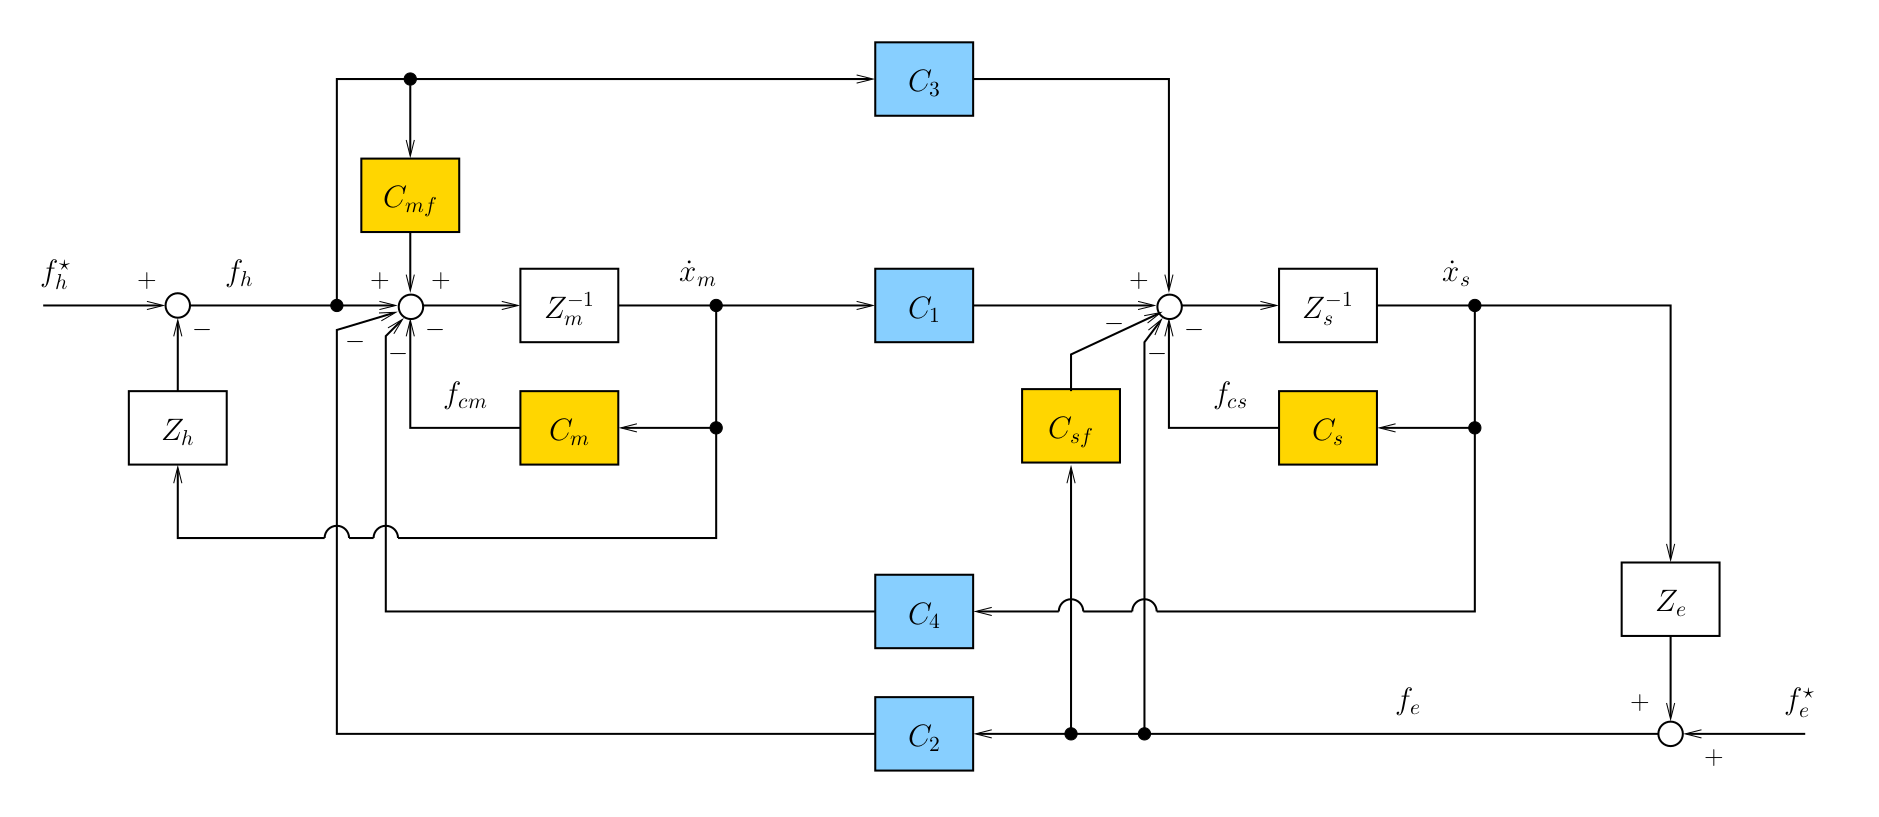
\includegraphics[scale=0.3]{images/four_channel.png}
    \end{center}
    \caption{4 Channel Bilateral Telemanipulation architecture with inner force loops $C_{mf}$ and $C_{sf}$.}
    \label{fig:four_channel}
\end{figure}

\subsection{Single-Input Single-Output implementation}
Implement the SISO Four-channel bilateral teleoperation architecture with
\[
    C_m = B_m + \frac{K_m}{s} \quad
    C_s = B_s + \frac{K_s}{s}
\]
\[
    Z_m^{-1} = \frac{1}{M_ms + D_m} \quad
    Z_s^{-1} = \frac{1}{M_ss + D_s}
\]

\bigskip
\noindent where $Mm = 0.5$, $M_s = 2$. Moreover $D_s = 10$ and $D_m = 5$ or both zero in the initial case. In Fig \ref{fig:four_free} a simple plot of the positions and velocities (slave and master) are reported for proper selected tuning parameters of the related master and slave controller. In order to properly tune the controllers the following closed-loop systems were considered:

\[
G_m = \frac{1}{M_ms^2+B_ms+K_m} \quad
G_s = \frac{1}{M_ss^2+B_ss+K_s}
\]

\begin{figure}[H]
    \begin{center}
        \hspace*{-4.4cm}
        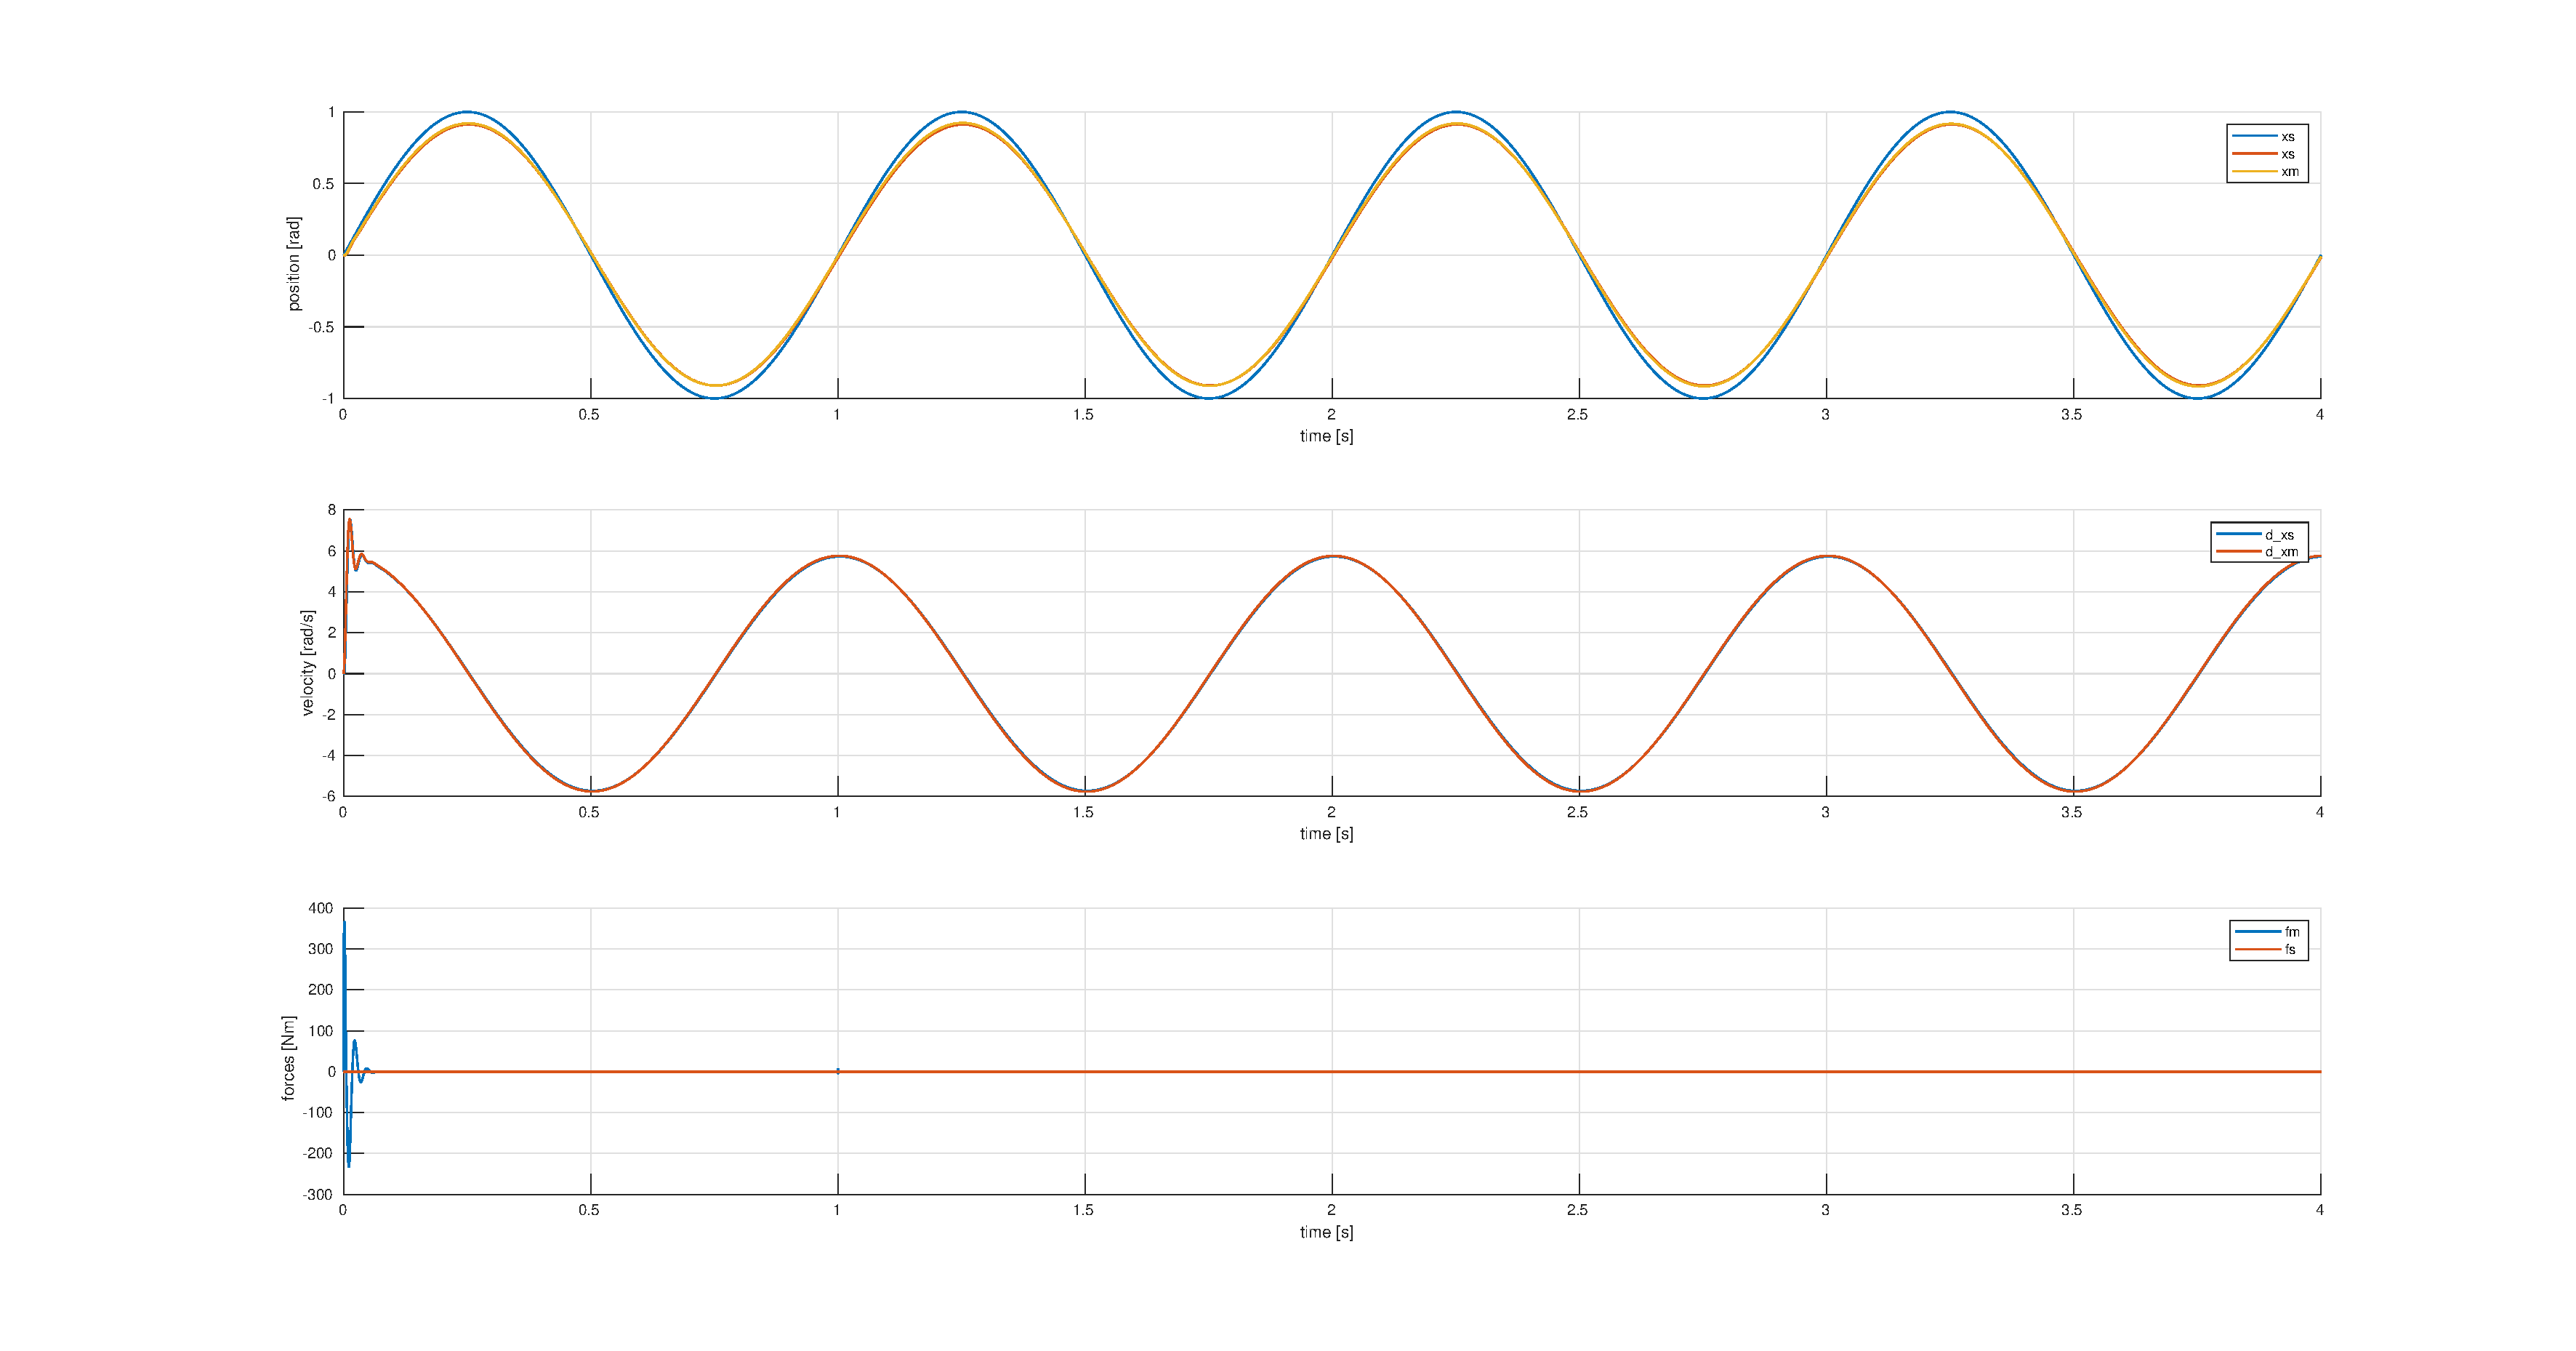
\includegraphics[scale=0.5]{images/four_free_motion.eps}
    \end{center}
    \caption{4 channel architecture in free motion with a sinusoidal reference}
    \label{fig:four_free}
\end{figure}

\bigskip
\noindent The proper parameters were selected considering the step response of the two second order systems. For the human intention controller the parameters were selected by comparing the reference position with the master/slave position and perform proper tuning (an analytical closed-loop system might also be considered for this analysis).

\bigskip
The environment is a pure stiffness $K_e = 200$ but also other scenario has been considered. The reference is sinusoidal function with unitary amplitude and frequency 0.1Hz

\begin{figure}[H]
    \begin{center}
        \hspace*{-4.4cm}
        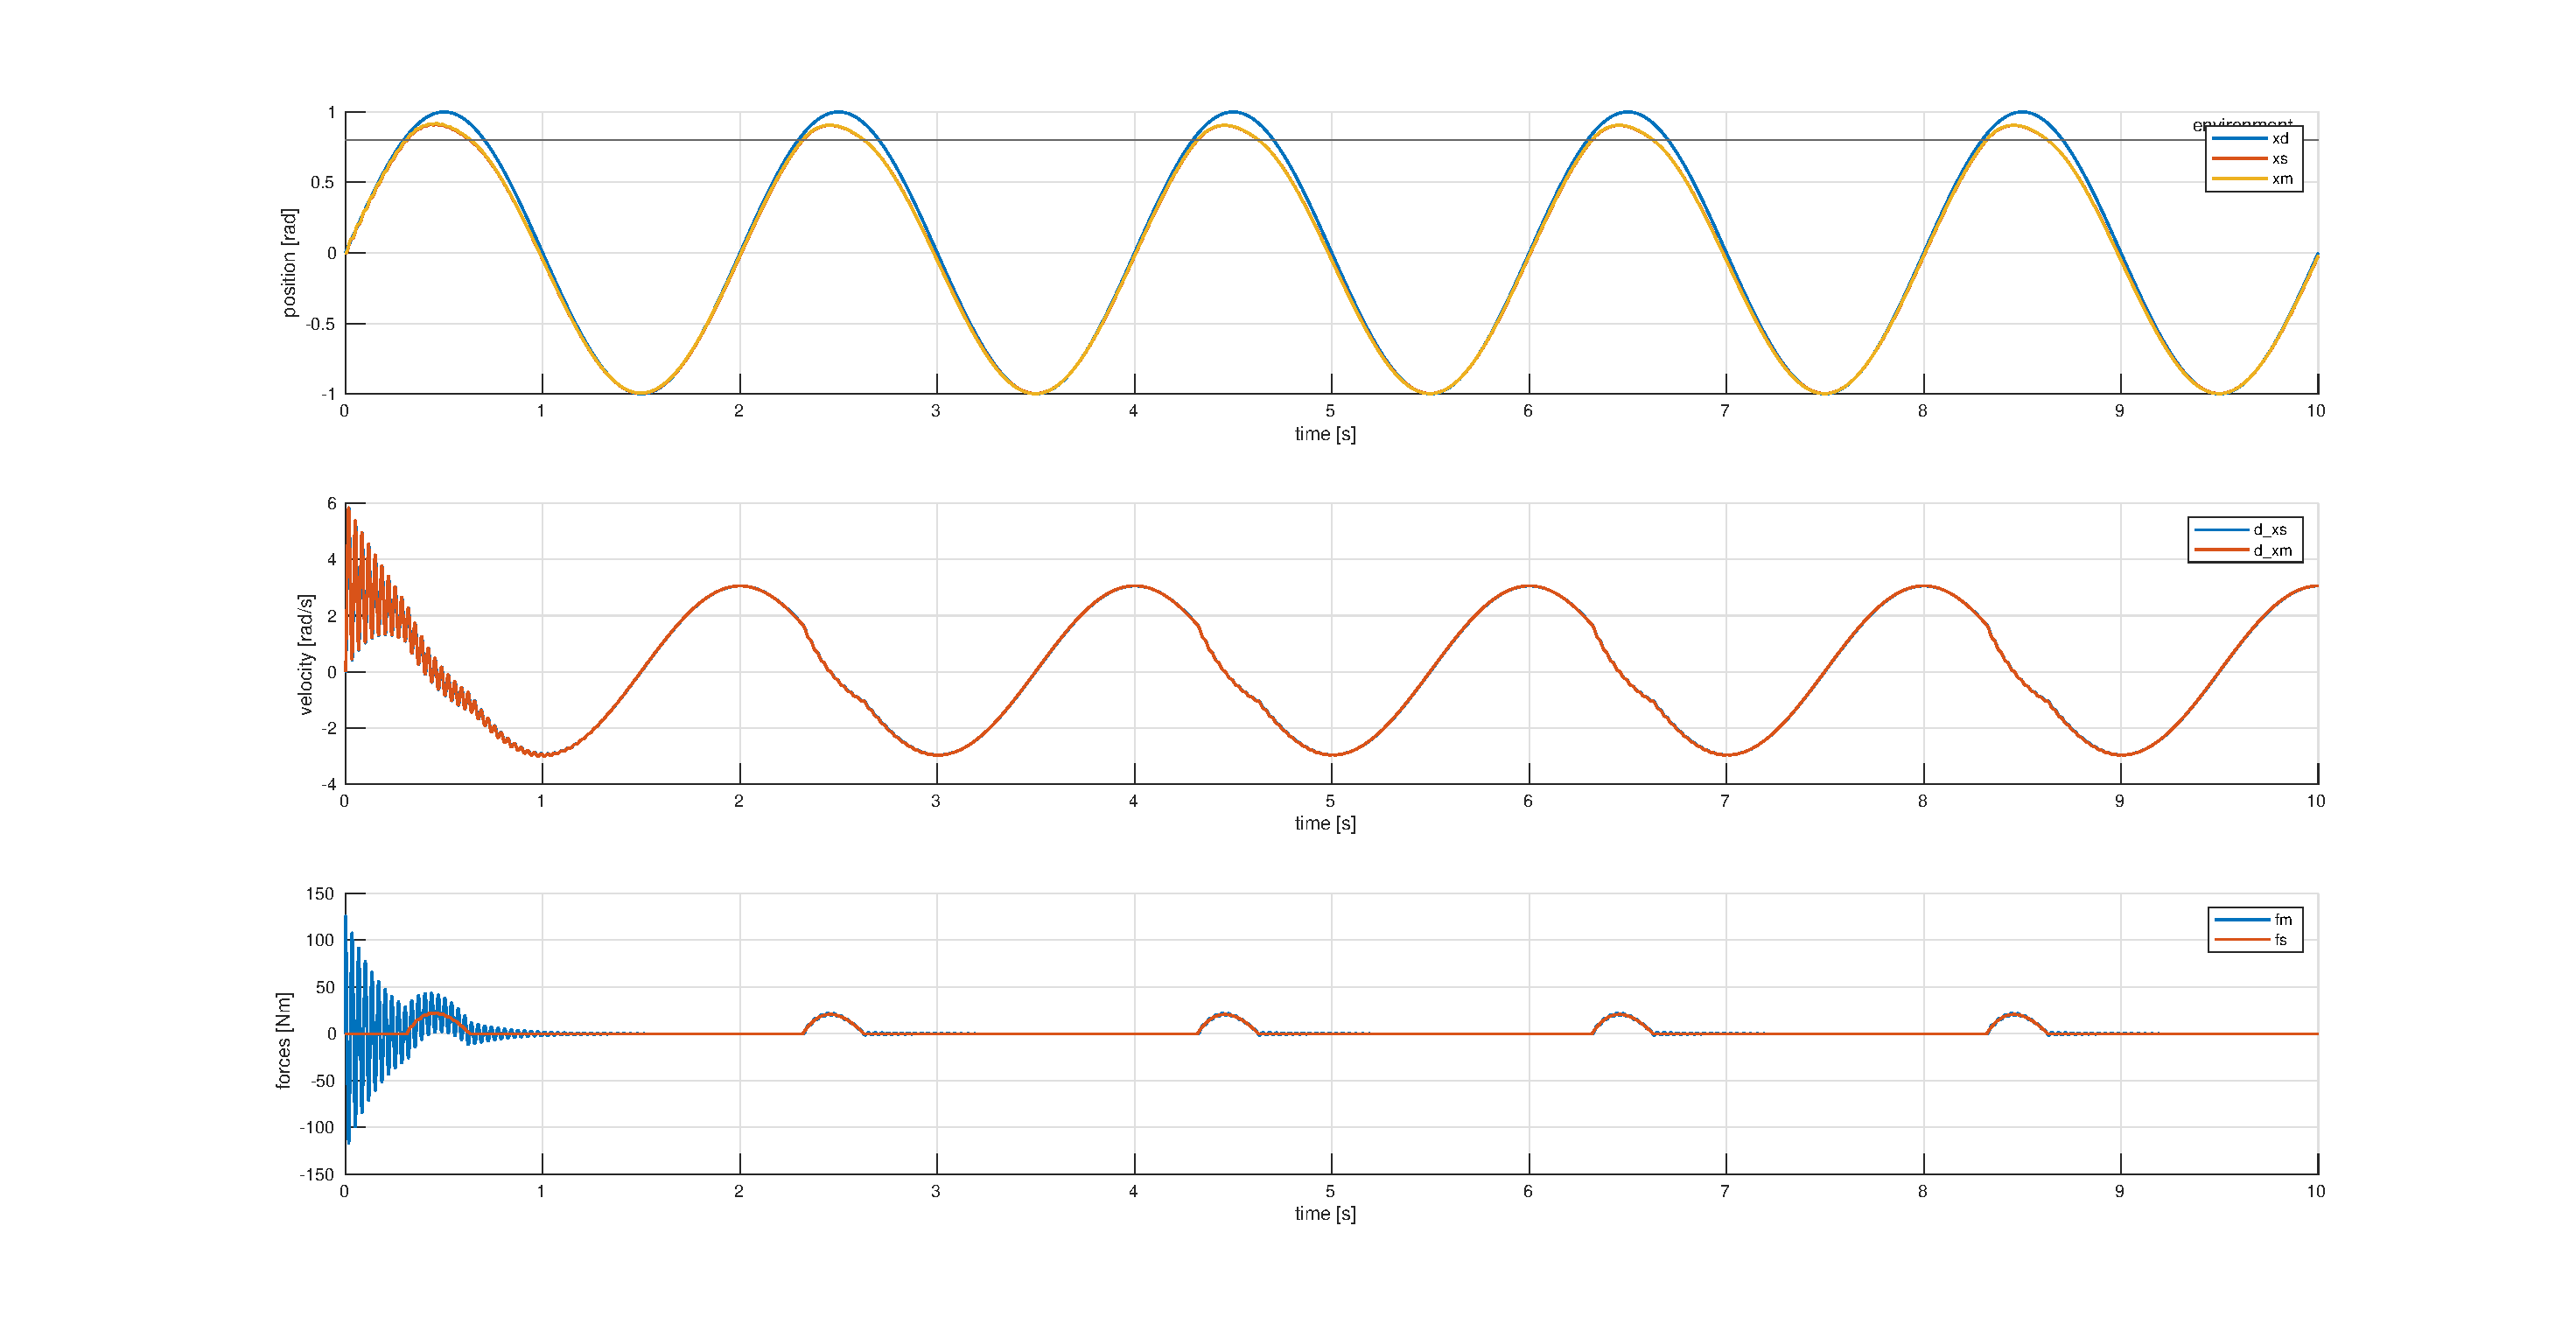
\includegraphics[scale=0.5]{images/four_contact_05.eps}
    \end{center}
    \caption{4 channel architecture in contact at 0.8 with a sinusoidal reference}
    \label{fig:four_cotact}
\end{figure}

In Fig \ref{fig:four_cotact} it is visible the transparency effect at contact $f_e=f_h$. The initial oscillations come from the tuning of the human controller. As it is visible the environment changes the behavior of the master if we compare it with Fig \ref{fig:four_free}.

\begin{figure}[H]
    \begin{center}
        \hspace*{-4.4cm}
        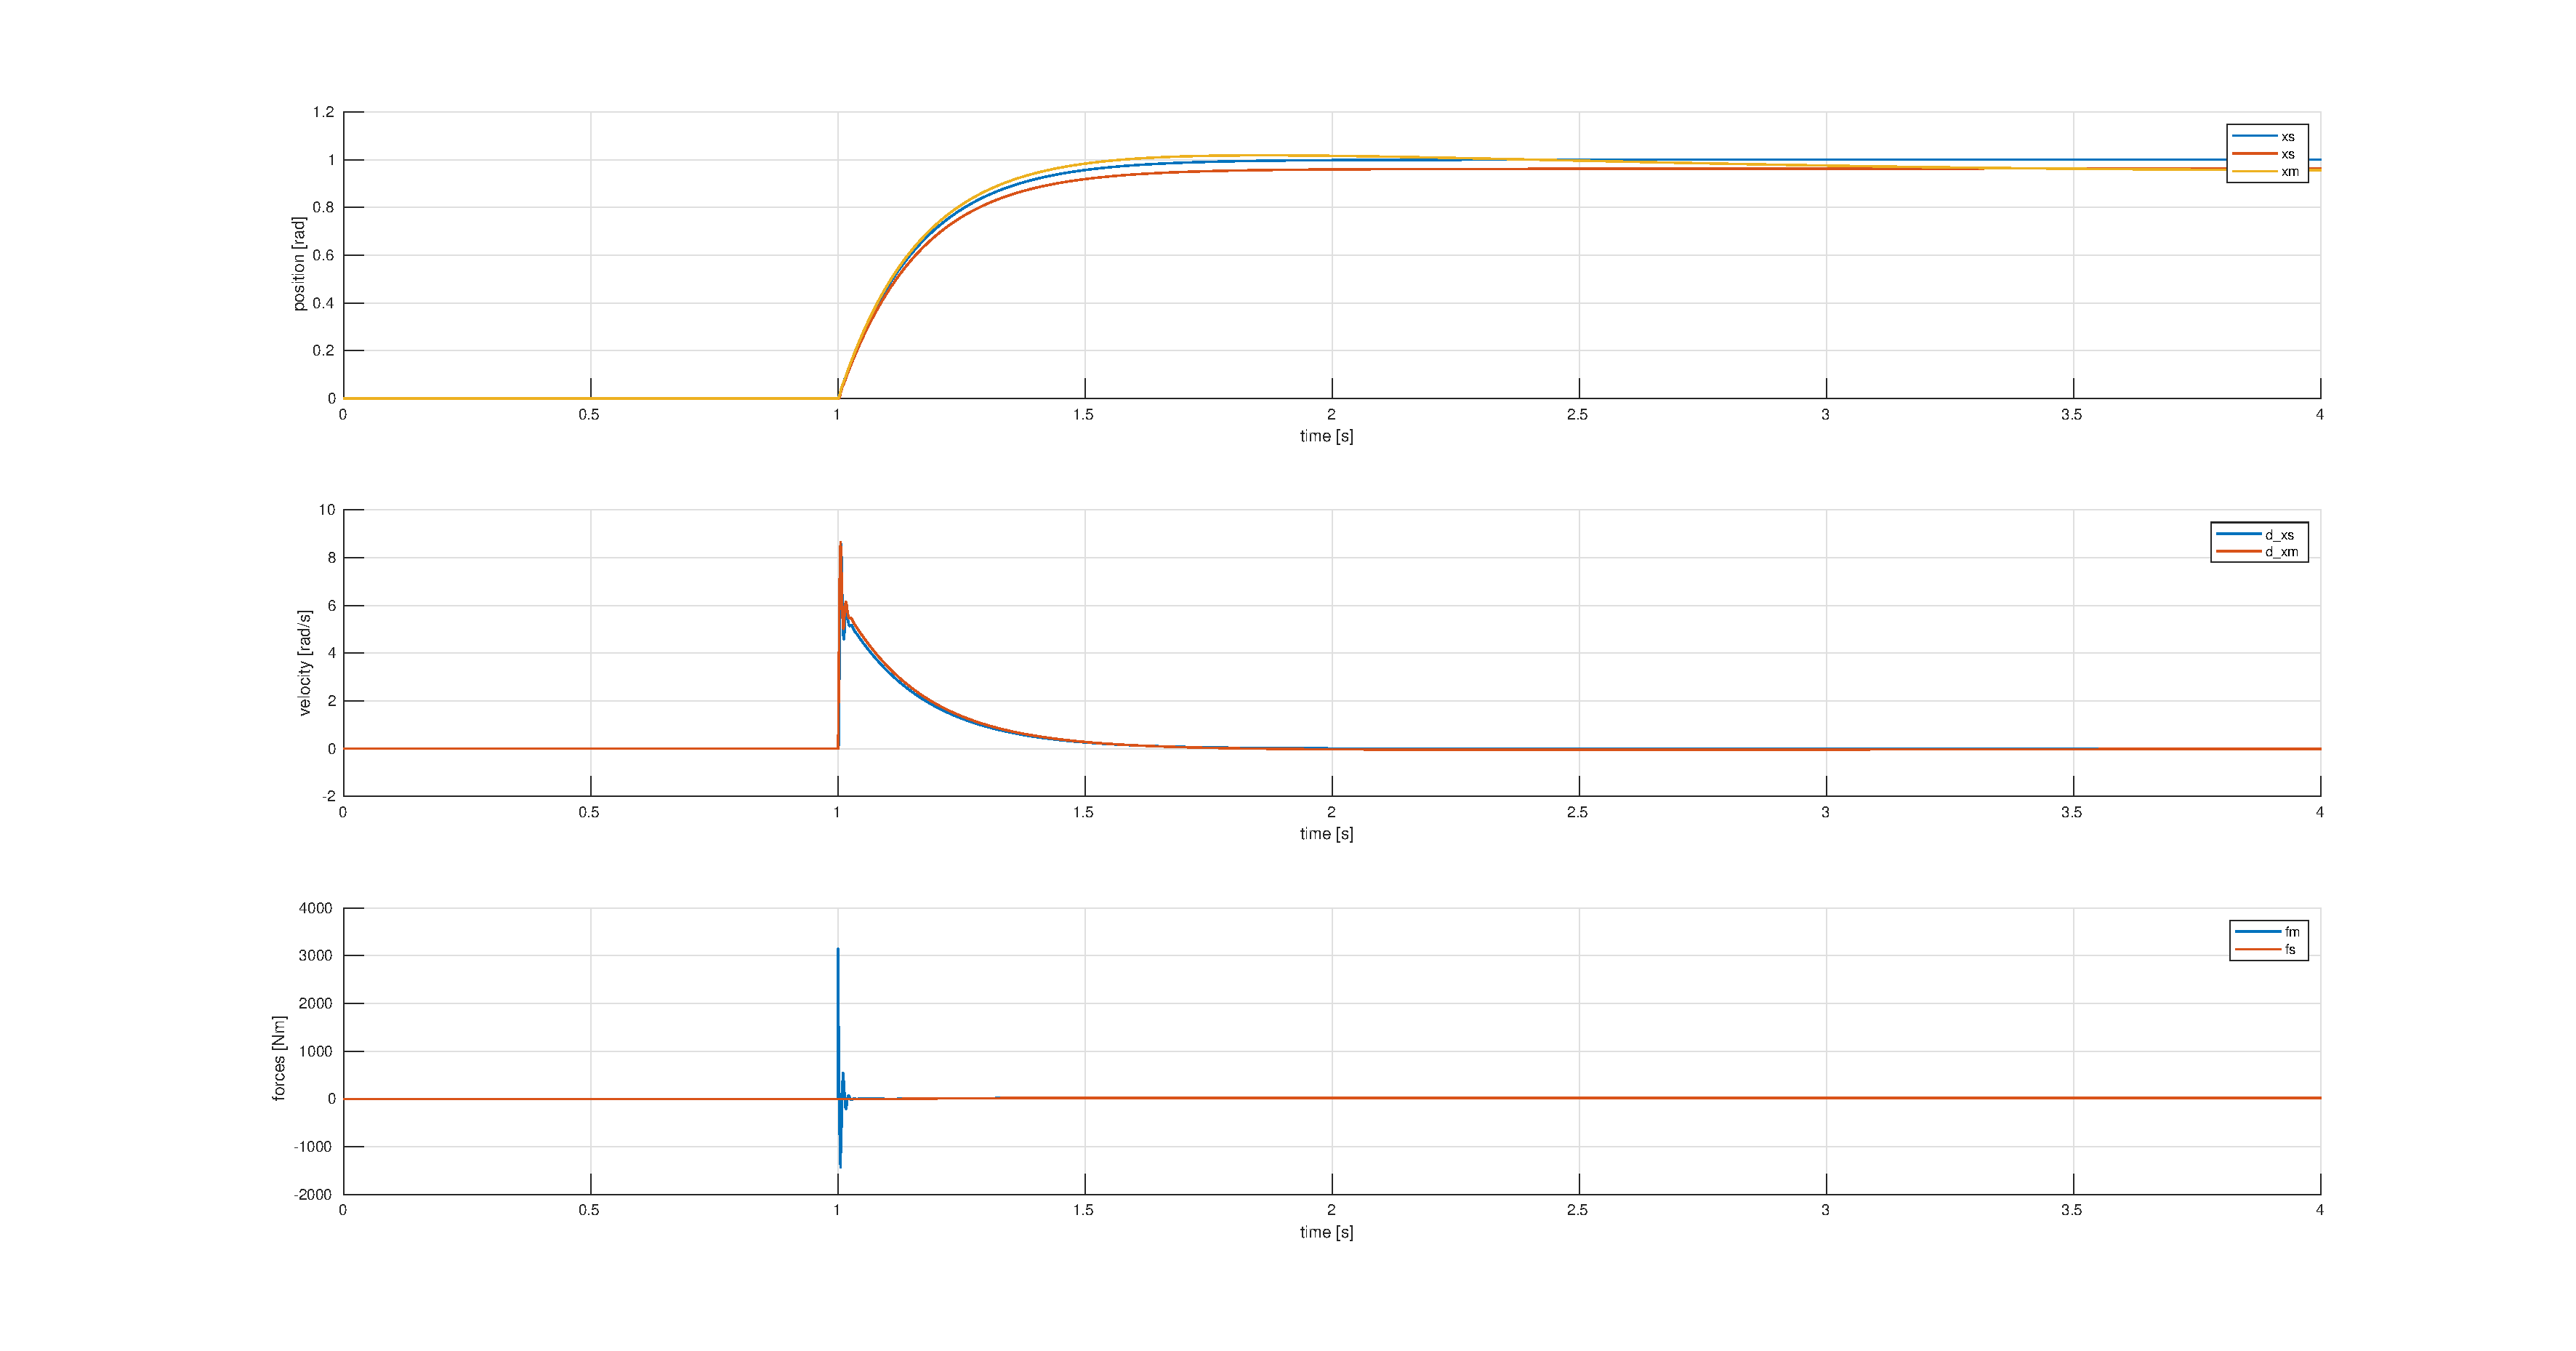
\includegraphics[scale=0.5]{images/four_step_contact_05.eps}
    \end{center}
    \caption{4 channel architecture in contact at 0.8 with a step reference}
    \label{fig:four_step}
\end{figure}

As it is visible in Fig \ref{fig:four_free} the architecture is correctly following the reference provided. There is however a large effect due to the initial motion in all the presented figures due to high gain. In Fig \ref{fig:four_cotact} the contact interaction is clearly visible in the forces plot when the position reaches 0.8. 

Finally the Fig \ref{fig:four_step} gives an idea of the response of the system to a step function and Fig \ref{fig:four_noisy} emphasizes the problem related to estimation of velocity and accelerations with noisy measurements. Moreover the inner force feedback can be introduced as constants and be properly tuned as desired.

\begin{figure}[H]
    \begin{center}
        \hspace*{-4.2cm}
        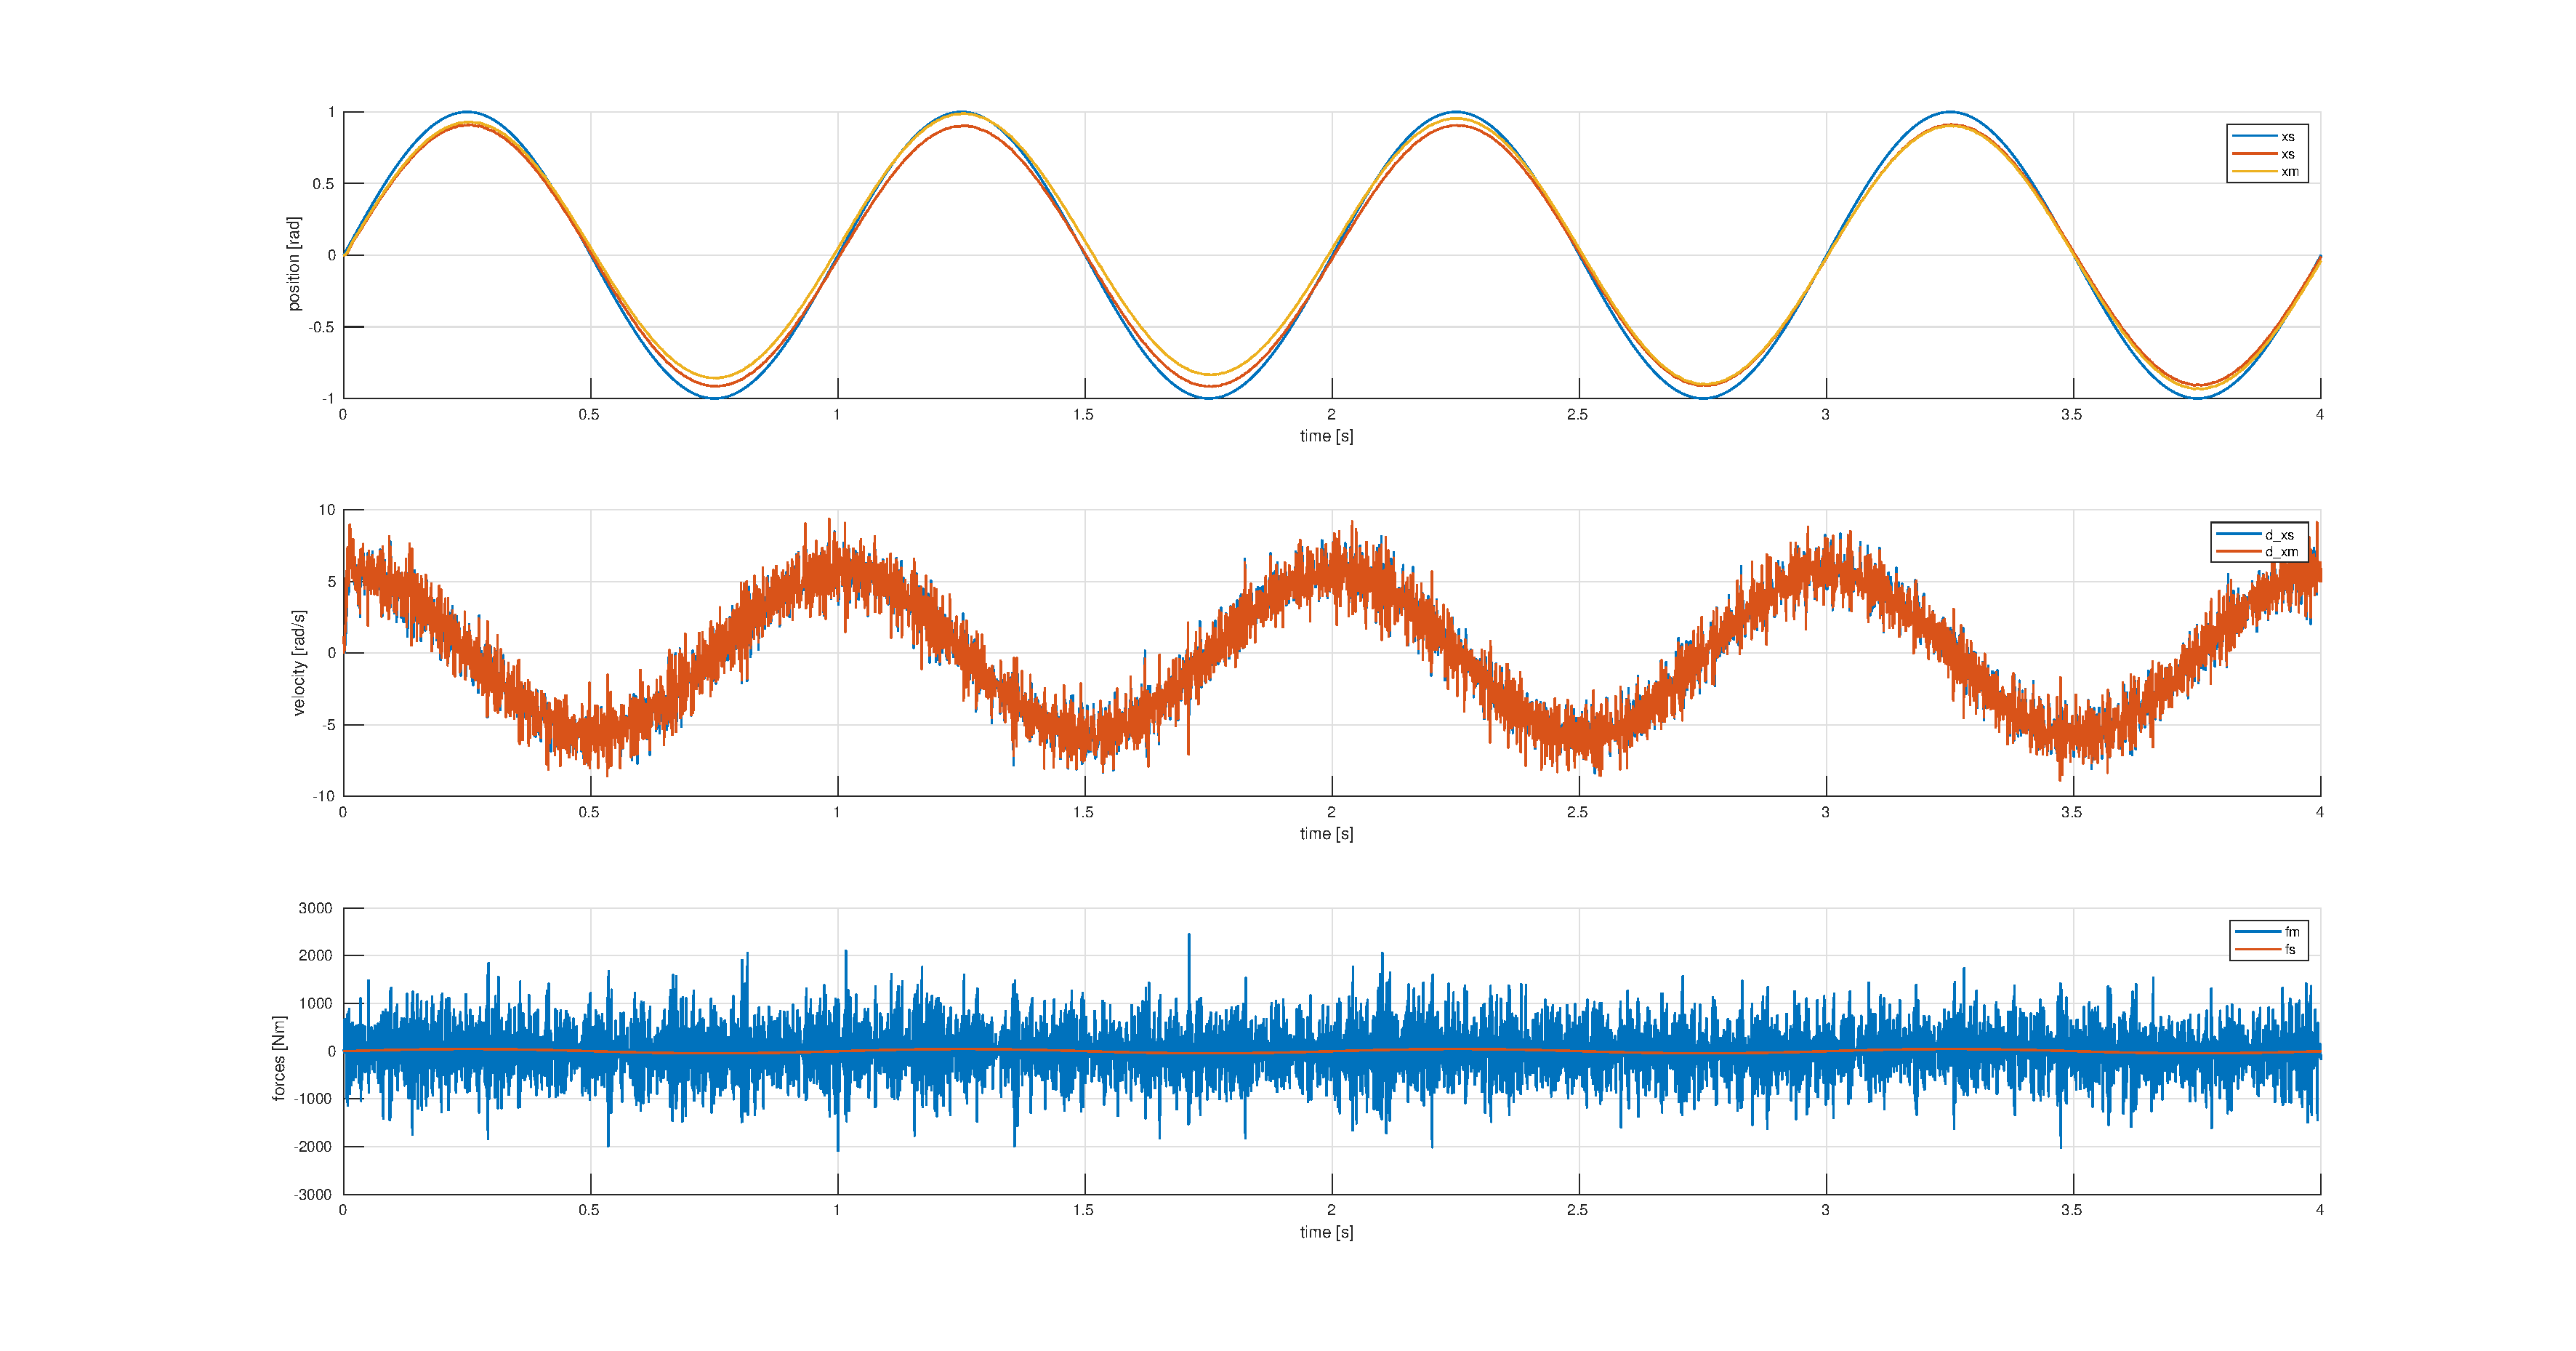
\includegraphics[scale=0.4]{images/four_noisy.eps}
    \end{center}
    \caption{Four channel architecture with white noise. The sinusoidal reference is much faster in this case}
    \label{fig:four_noisy}
\end{figure}

\noindent The entire architecture was translated in the related discretized version according to our specification in terms of encoders and the related derivative were performed using the simulink block. In the following section kalman filters will be introduced and they will be used to filter noisy estimations of velocities and accelerations.


\begin{figure}[H]
    \begin{center}
        \hspace*{-4.2cm}
        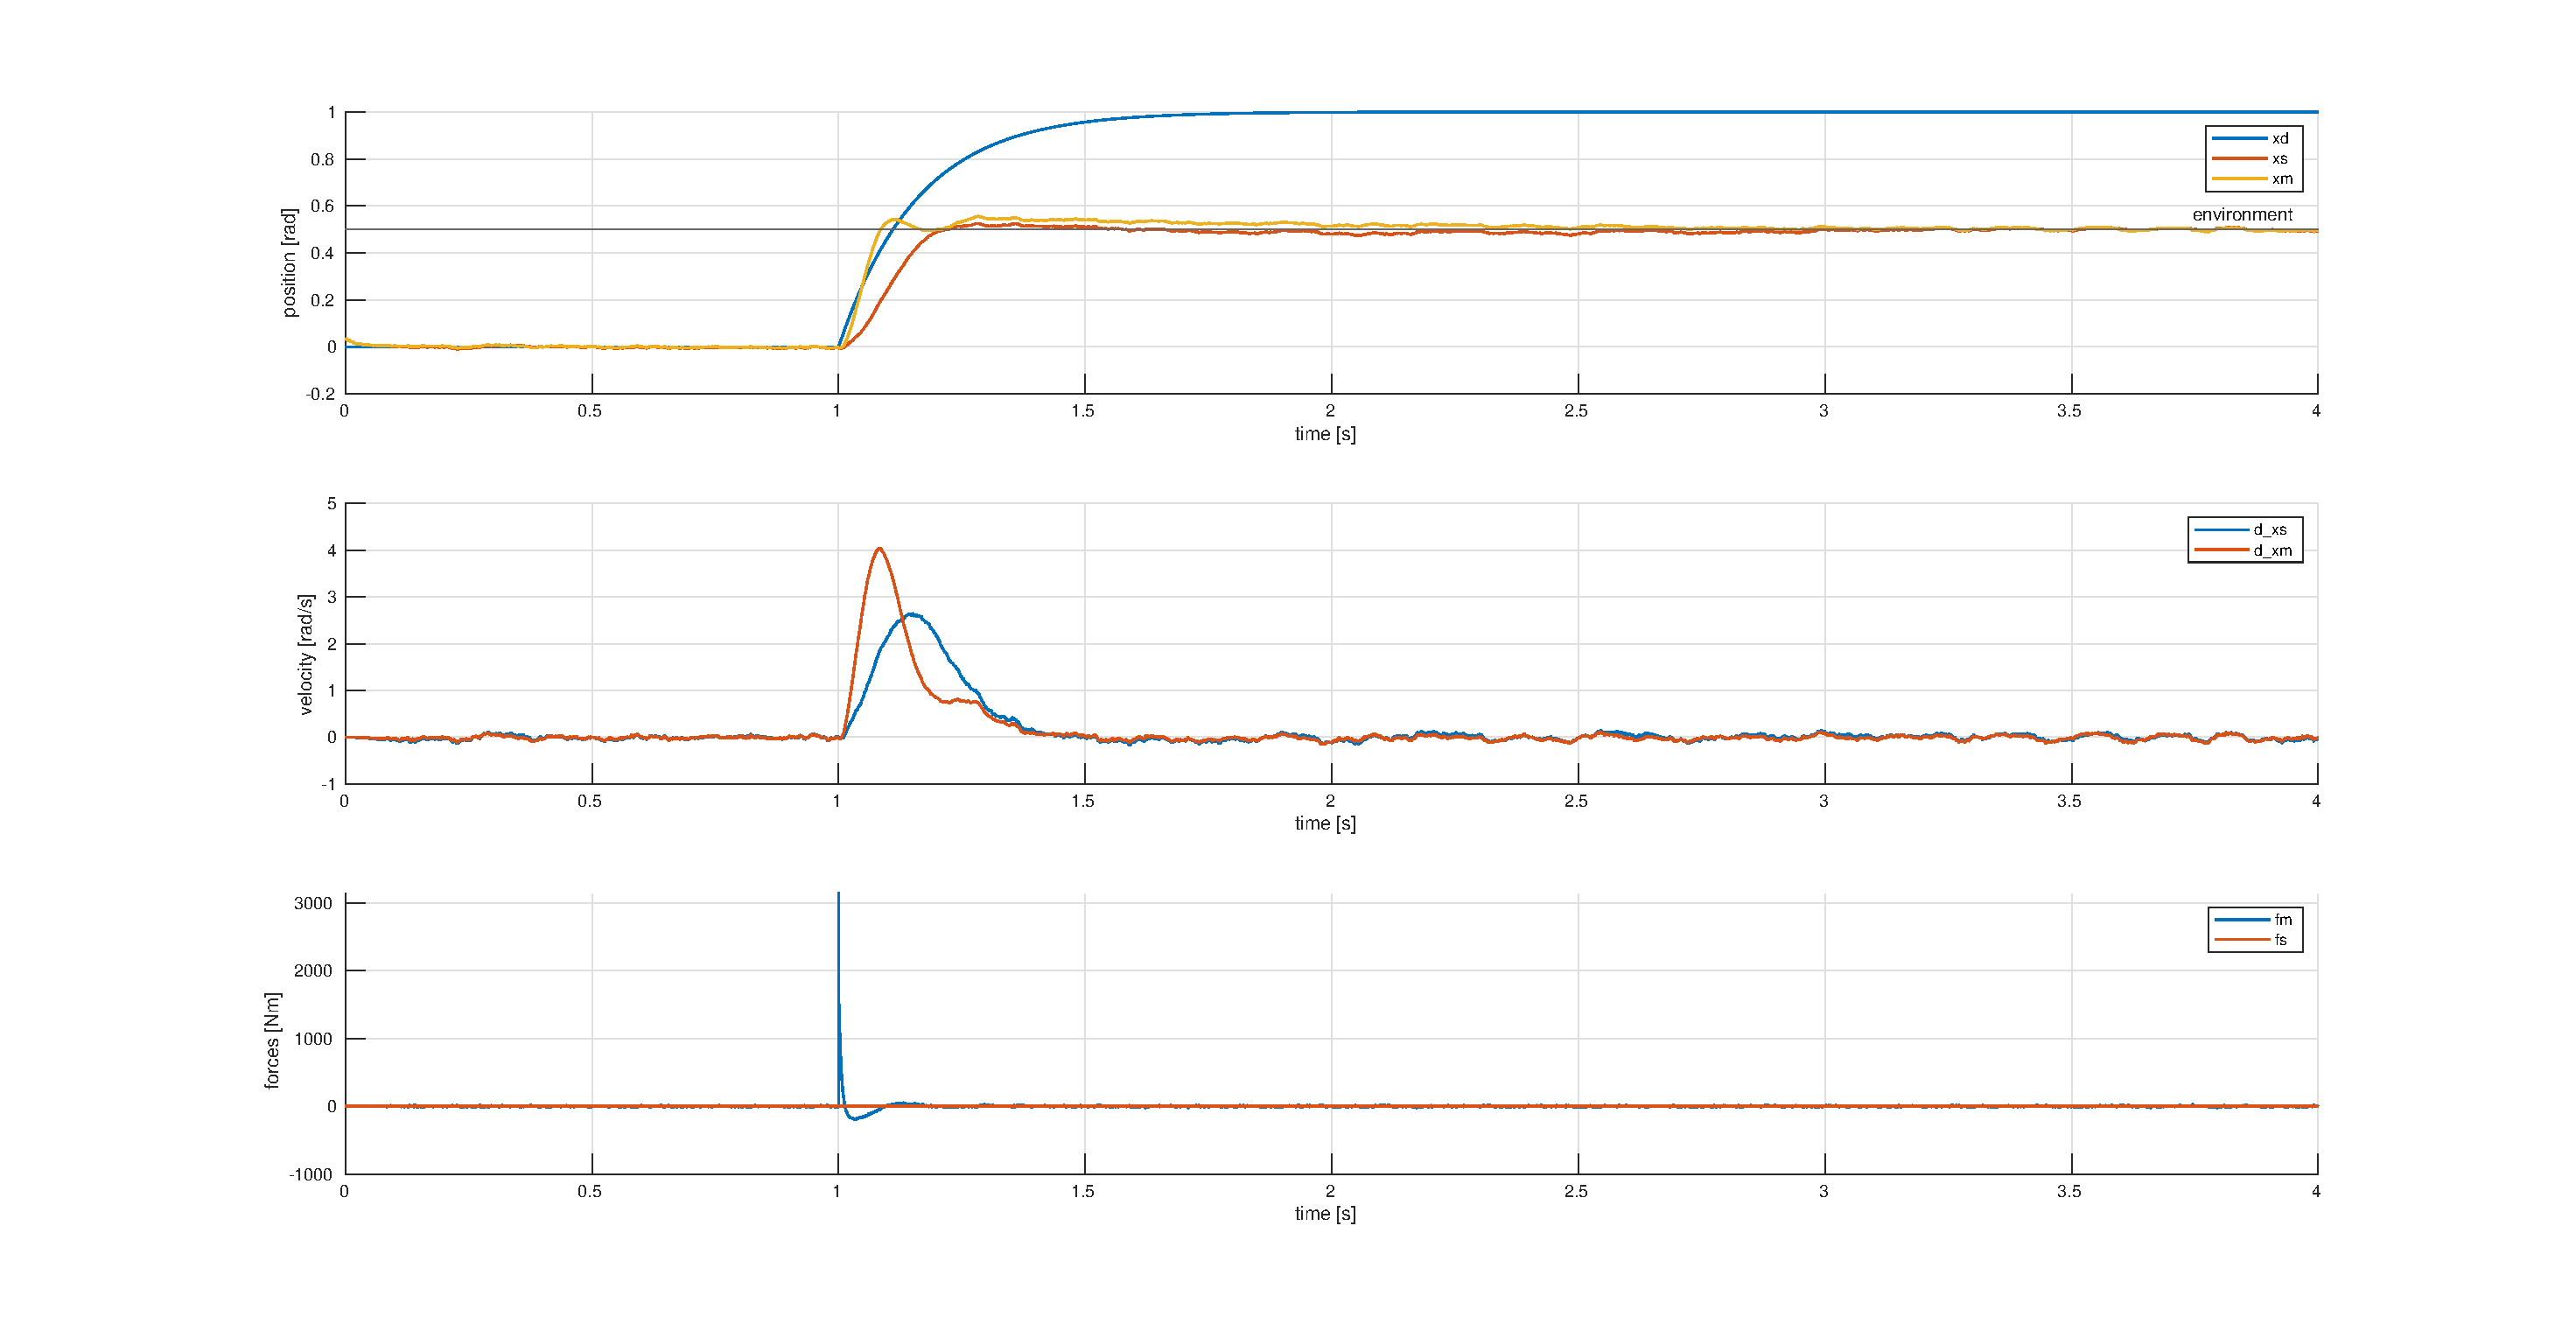
\includegraphics[scale=0.5]{images/four_step_kalman_2.eps}
    \end{center}
    \caption{Four channel architecture with white noise. The sinusoidal reference is much faster in this case}
    \label{fig:four_noisy}
\end{figure}

\bigskip
\noindent The inner force loops in this architecture don't produce really different results so the related plots are not reported. 

\subsection{Derive the Lawrence hybrid matrix}

Derive the hybrid matrix for the four channel bilateral teleoperation considering the inner force loop at the master and slave side. We can directly consider Fig \ref{fig:four_channel}.

\[
\begin{bmatrix}  f_m \\ -v_s \end{bmatrix} = \begin{bmatrix}
    \overline{H_{11}} & \overline{H_{12}} \\
    \overline{H_{21}} &  \overline{H_{22}} \\
\end{bmatrix} = \begin{bmatrix}  v_m \\ f_s \end{bmatrix}
\]

\noindent Let's start by defining:
\begin{equation}
    v_m = Z_{cm}^{-1}(f_m -C_2f_s-C_4v_s+C_{mf}f_m)
\end{equation}
\begin{equation}
    v_s = Z_{cs}^{-1}(-f_s -C_{sf}f_s+C_1v_m+C_3f_m)
\end{equation}

\noindent Finally let's compute the 4 components of the hybrid matrix considering one component to zero at each step.
\[
    \overline{H_{11}} : f_m \rightarrow v_m \qquad f_s = 0
    \]\[
    Z_{cm}v_m = f_m - C_4Z_{cs}^{-1}C_1v_m - C_4Z_{cs}^{-1}C_3f_m + C_{mf}f_m
\]\[
    v_m(Z_{cm}+C_4Z_{cs}^{-1}C_1) = f_m(1-C_4Z_{cs}^{-1}C_3 + C_{mf})
    \]\[
    \overline{H_{11}} = \frac{Z_{cm}Z_{cs}+C_1C_4}{(1+C_{mf})Z_{cs} - C_3C_4}
\]


\bigskip

\[
    \overline{H_{12}} : f_m \rightarrow f_s \qquad v_m = 0
    \]\[
    0 = f_m -C_2f_s +C_4Z_{cs}^{-1}C_{sf}f_s + C_4Z_{cs}^{-1}f_s - C_{mf}f_m
\]\[
    f_m(1-C_{mf}-C_4Z_{cs}^{-1}C_3) = f_s(C_2-C_4Z_{cs}^{-1}C_{sf}C_{sf}-C_4Z_{cs}^{-1})
    \]\[
    \overline{H_{12}} = \frac{C_2Z_{cs}-C_4(1+C_{sf})}{(1+C_{mf})Z_{cs} - C_3C_4}
\]

\bigskip

\[
    \overline{H_{21}} : -v_s \rightarrow v_m \qquad f_s = 0
    \]\[
    v_sZ_{cs} = -(C_1v_m + C_3f_m)
\]\[
    v_s(Z_{cs} - \frac{C_3C_4}{1+C_{mf}} = -v_m(C_1 + \frac{C_3Z_{cm}}{1+C_{mf}})
    \]\[
    \overline{H_{21}} = -\frac{C_1(1+C_{mf}) + C_3Z_{cm}}{(1+C_{mf})Z_{cs} - C_3C_4}
\]


\bigskip

\[
    \overline{H_{22}} : -v_s \rightarrow f_s \qquad v_m = 0
\]\[
    v_sZ_{cs} = C_{sf}f_s + f_s + C_{sf}f_s
\]\[
    v_s(Z_{cs}-\frac{C_3C_4}{1+C_{mf}}) = f_s(C_{sf} + 1 - \frac{C_3C_2}{1+C_{mf}})
\]\[
    \overline{H_{22}} = \frac{(1+C_{sf})(1+C_{mf})-C_2C_3}{(1+C_{mf})Z_{cs}-C_3C_4}
\]

\subsection{Derive the Hannaford hybrid matrix}
Derive the hybrid matrix H for the four channel bilateral teleoperation considering the inner force loop at the master and slave side. We can directly consider Fig \ref{fig:four_channel}.

\[
\begin{bmatrix}  f_m \\ v_m \end{bmatrix} = \begin{bmatrix}
    H_{11} & H_{12} \\
    H_{21} & H_{22} \\
\end{bmatrix} = \begin{bmatrix}  v_s \\ -f_s \end{bmatrix}
\]

\noindent Let's start by defining:
\begin{equation}
    v_m = Z_{m}^{-1}(f_m(1+C_{mf}) - C_2f_s - C_4v_s-v_mC_m)
\end{equation}
\begin{equation}
    v_s = Z_{s}^{-1}(v_mC_1 + f_mC_3 - f_s(C_{sf}+1) - v_sC_s)
\end{equation}

\noindent Finally let's compute the 4 components of the hybrid matrix considering one component to zero at each step.
\[
    H_{11} : f_m \rightarrow v_s \qquad f_s = 0
    \]\[
    (Z_m + C_m)v_m = f_m(1+C_{mf}) - C_4v_s \qquad \text{from (3)}
\]\[
    H_{11} = \frac{(Z_s+C_s)(Z_m+C_m) +C_4C_1}{C_1(1+C_{mf}) + C_3(Z_m+C_m)}  \qquad \text{by (4) for removing } v_m
\]


\bigskip

\[
    H_{12} : f_m \rightarrow -f_s \qquad v_s = 0
    \]\[
        (Z_m + C_m)v_m = f_m(1+C_{mf}) - C_2f_s \qquad \text{from (3)}
\]\[
    H_{12} = \frac{-(1+C_{sf})(Z_m+C_m) - C_2C_1}{C_1(1+C_mf)+C_3(Z_m+C_m)} \qquad \text{by (4) for removing } v_m
\]

\bigskip

\[
    H_{21} : v_m \rightarrow v_s \qquad f_s = 0
    \]\[
    (1+C_{mf})f_m = v_m(Z_m + C_m) + C_4v_s \qquad \text{from (3)}
\]\[
    H_{21} = \frac{(1+C_{mf})(Z_s + C_s) - C_3C_4}{C_3(Z_m + C_m)+ C_1(1+C_mf)} \qquad \text{by (4) for removing } f_m
\]


\bigskip

\[
    H_{22} : v_m \rightarrow -f_s \qquad v_s = 0
\]\[
    (1+C_{mf})f_m = v_m(Z_m + C_m) + C_2f_s \qquad \text{from (3)}
\]\[
    H_{22} = \frac{C_2C_3 - (1+C_{mf})(1+C_{sf})}{C_1(1+C_{mf}) + C_3(Z_m+C_m)}  \qquad \text{by (4) for  removing } f_m
\]

\section{Kalman Filter, Predictor and Smoother}
In this section we are briefly going to consider the following estimation problems:
\begin{itemize}
    \item \textbf{Filtering} estimate $\hat{s}(t)$ using measurements till time t
    \item \textbf{Prediction}: estimate $\hat{s}(t+h)$ using measurements till time t
    \item \textbf{Smoothing}: estimate $\hat{s}(t-h)$ using measurements till time t
\end{itemize}
\bigskip

Our aim is to estimate the velocities and accelerations from noisy position measurements. Some samples were provided for the task and the kalman filter and predictor were implemented as well as the steady state versions. The theory behind the kalman filter and predictor is not fully reported. Let's derive the discrete-time model for the position, velocities and accelerations to use in the kalman filter:

\begin{equation}
    \dot{x}(t) =  \begin{bmatrix}  0&1&0 \\ 0&0&1\\0&0&0 \end{bmatrix} x(t) + \begin{bmatrix}  0\\0\\1 \end{bmatrix} w(t)
    \qquad
    y(t) = \begin{bmatrix}  1&0&0 \end{bmatrix}x(t) + v(t)
\end{equation}

\noindent Let's compute the discrete-time model from the continuous-time model:
\[
    A_d = e^{AT_s} = e^{\begin{bmatrix}  0&1&0 \\ 0&0&1\\0&0&0 \end{bmatrix}T_s} = \begin{bmatrix} 1&T_s&\frac{T_s^2}{2}\\0&1&T_s\\0&0&1 \end{bmatrix}
\]
\[
    B_d = \int_{0}^{T_s} e^{\begin{bmatrix} 1&\tau&\tau^2/2\\0&1&\tau\\0&0&1 \end{bmatrix}} \,d\tau  = \begin{bmatrix} T_s^3/6\\T_s^2/2\\T_s \end{bmatrix}
\]
\[
    C_d = C = \begin{bmatrix} 1&0&0 \end{bmatrix}
\]

It is important to notice the presence of two variance matrixes $R$ related to $v_k$ and $Q$ related to $w_k$. The variance matrix $R$ also called noise variance depends on the sensors whereas the variance
matrix $Q$ also called model variance is chosen in order to explain the measurements as best as
possible. They are crucial for proper tuning of the kalman filter.

\bigskip
\noindent Briefly, the \textbf{kalman filter} can be defined using a recursive formulation composed of a prediction and an estimation step with proper initial conditions:
\[
    \hat{x}_{k+1|k+1} = A\hat{x}_{k|K} + K_{k+1}(y_{k-1} - CA\hat{x}_{k|k})
\]   
\[
    P_{k+1|k} = AP_{k|k-1}A^T - AP_{k|k-1}C^T(CP_{k|k-1}C^T + R)^{-1}CP_{k|k-1}A^T+Q
\]

\bigskip
where the kalman gain maps the output estimation error into the correction of the prediction state
\[
    K_{k+1} = P_{k+1|k}C^T(CP_{k+1|k}C^T+R)^{-1} \qquad \textbf{Kalman gain}
\]

when k goes to infinity we can consider the steady-state kalman filter which uses the Algebraic Ricati Equation (ARE) for getting $P_{\infty}$. Informally the steady-state kalman filter is not optimal at the beginning of the experiments but we can reach reasonable results. The entire formulations for the kalman predictor and smoother are not reported.

The parameters used are $q = 1000$, $R = 1$, $Q = qB_dB_d^T$, the initial state $x_0 = [pos; 0; 0]$ and the variance $P_0 = 0.1 \cdot eye(3)$.

\begin{figure}[H]
    \begin{center}
        \hspace*{-4.6cm}
        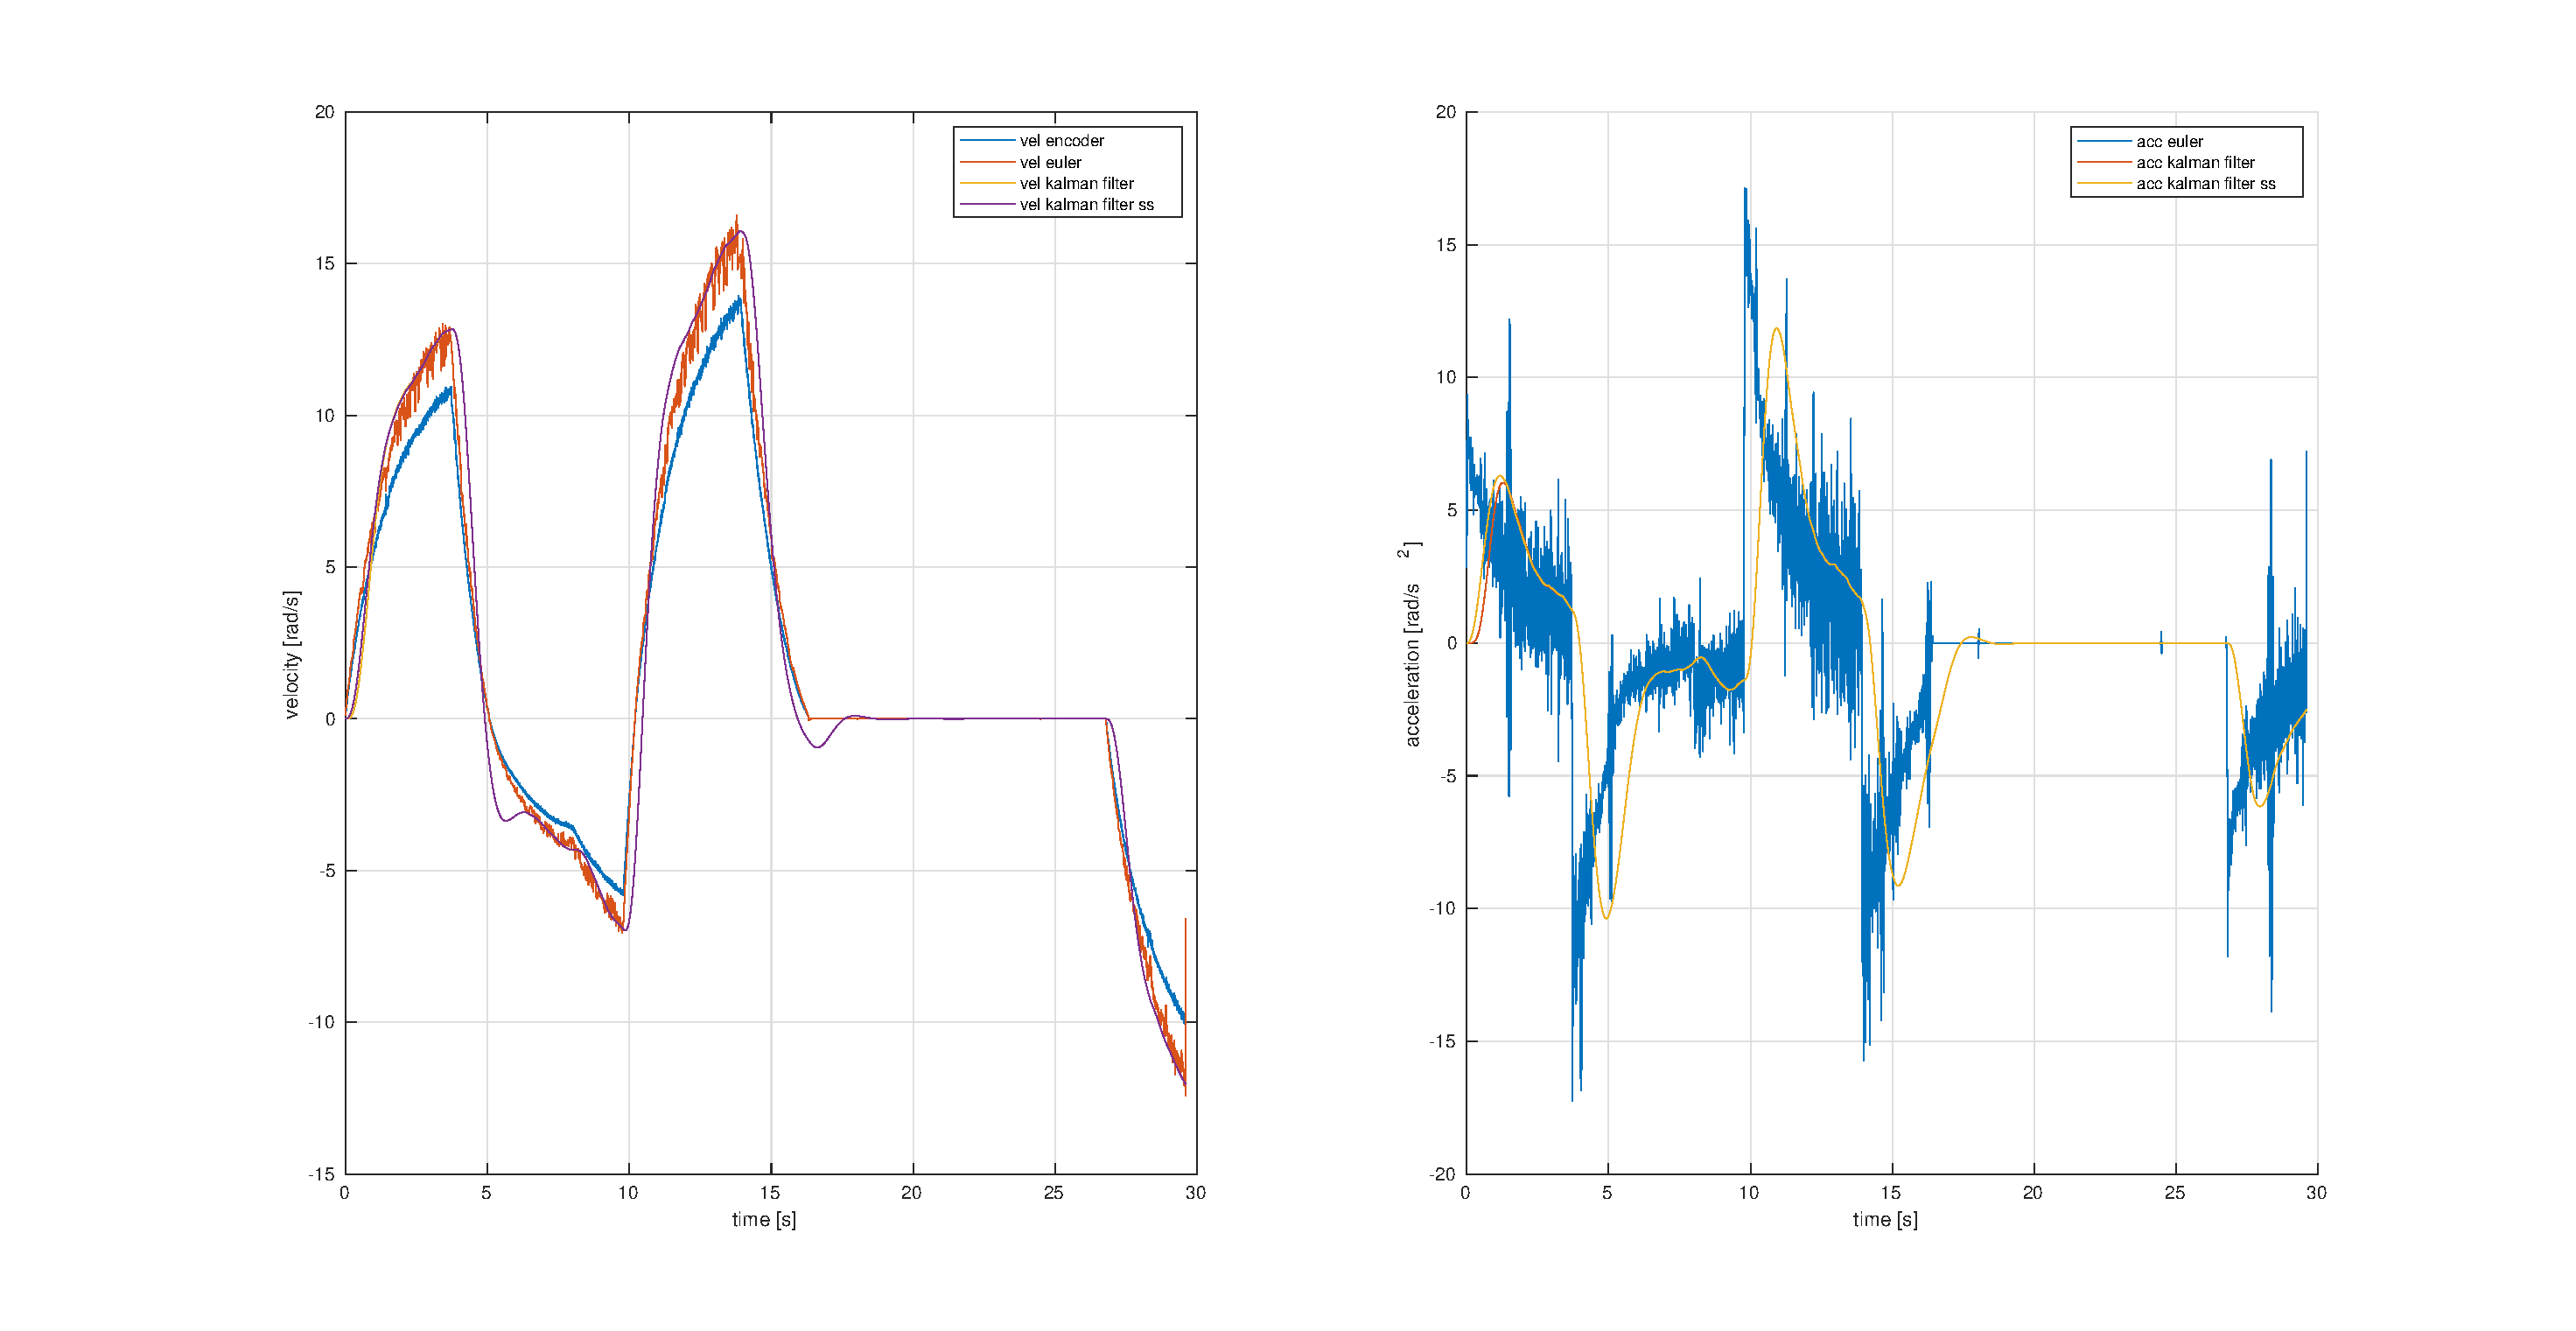
\includegraphics[scale=0.5]{images/kalman_filter.eps}
    \end{center}
    \caption{Velocities and accelerations estimations using Kalman filter, Kalman filter in steady state conditions and euler approximations with 5Hz low pass filter. As it is visible at the beginning the Kalman filter is different from the steady state version.}
    \label{fig:kalman_filter}
\end{figure}

\begin{figure}[H]
    \begin{center}
        \hspace*{-4.6cm}
        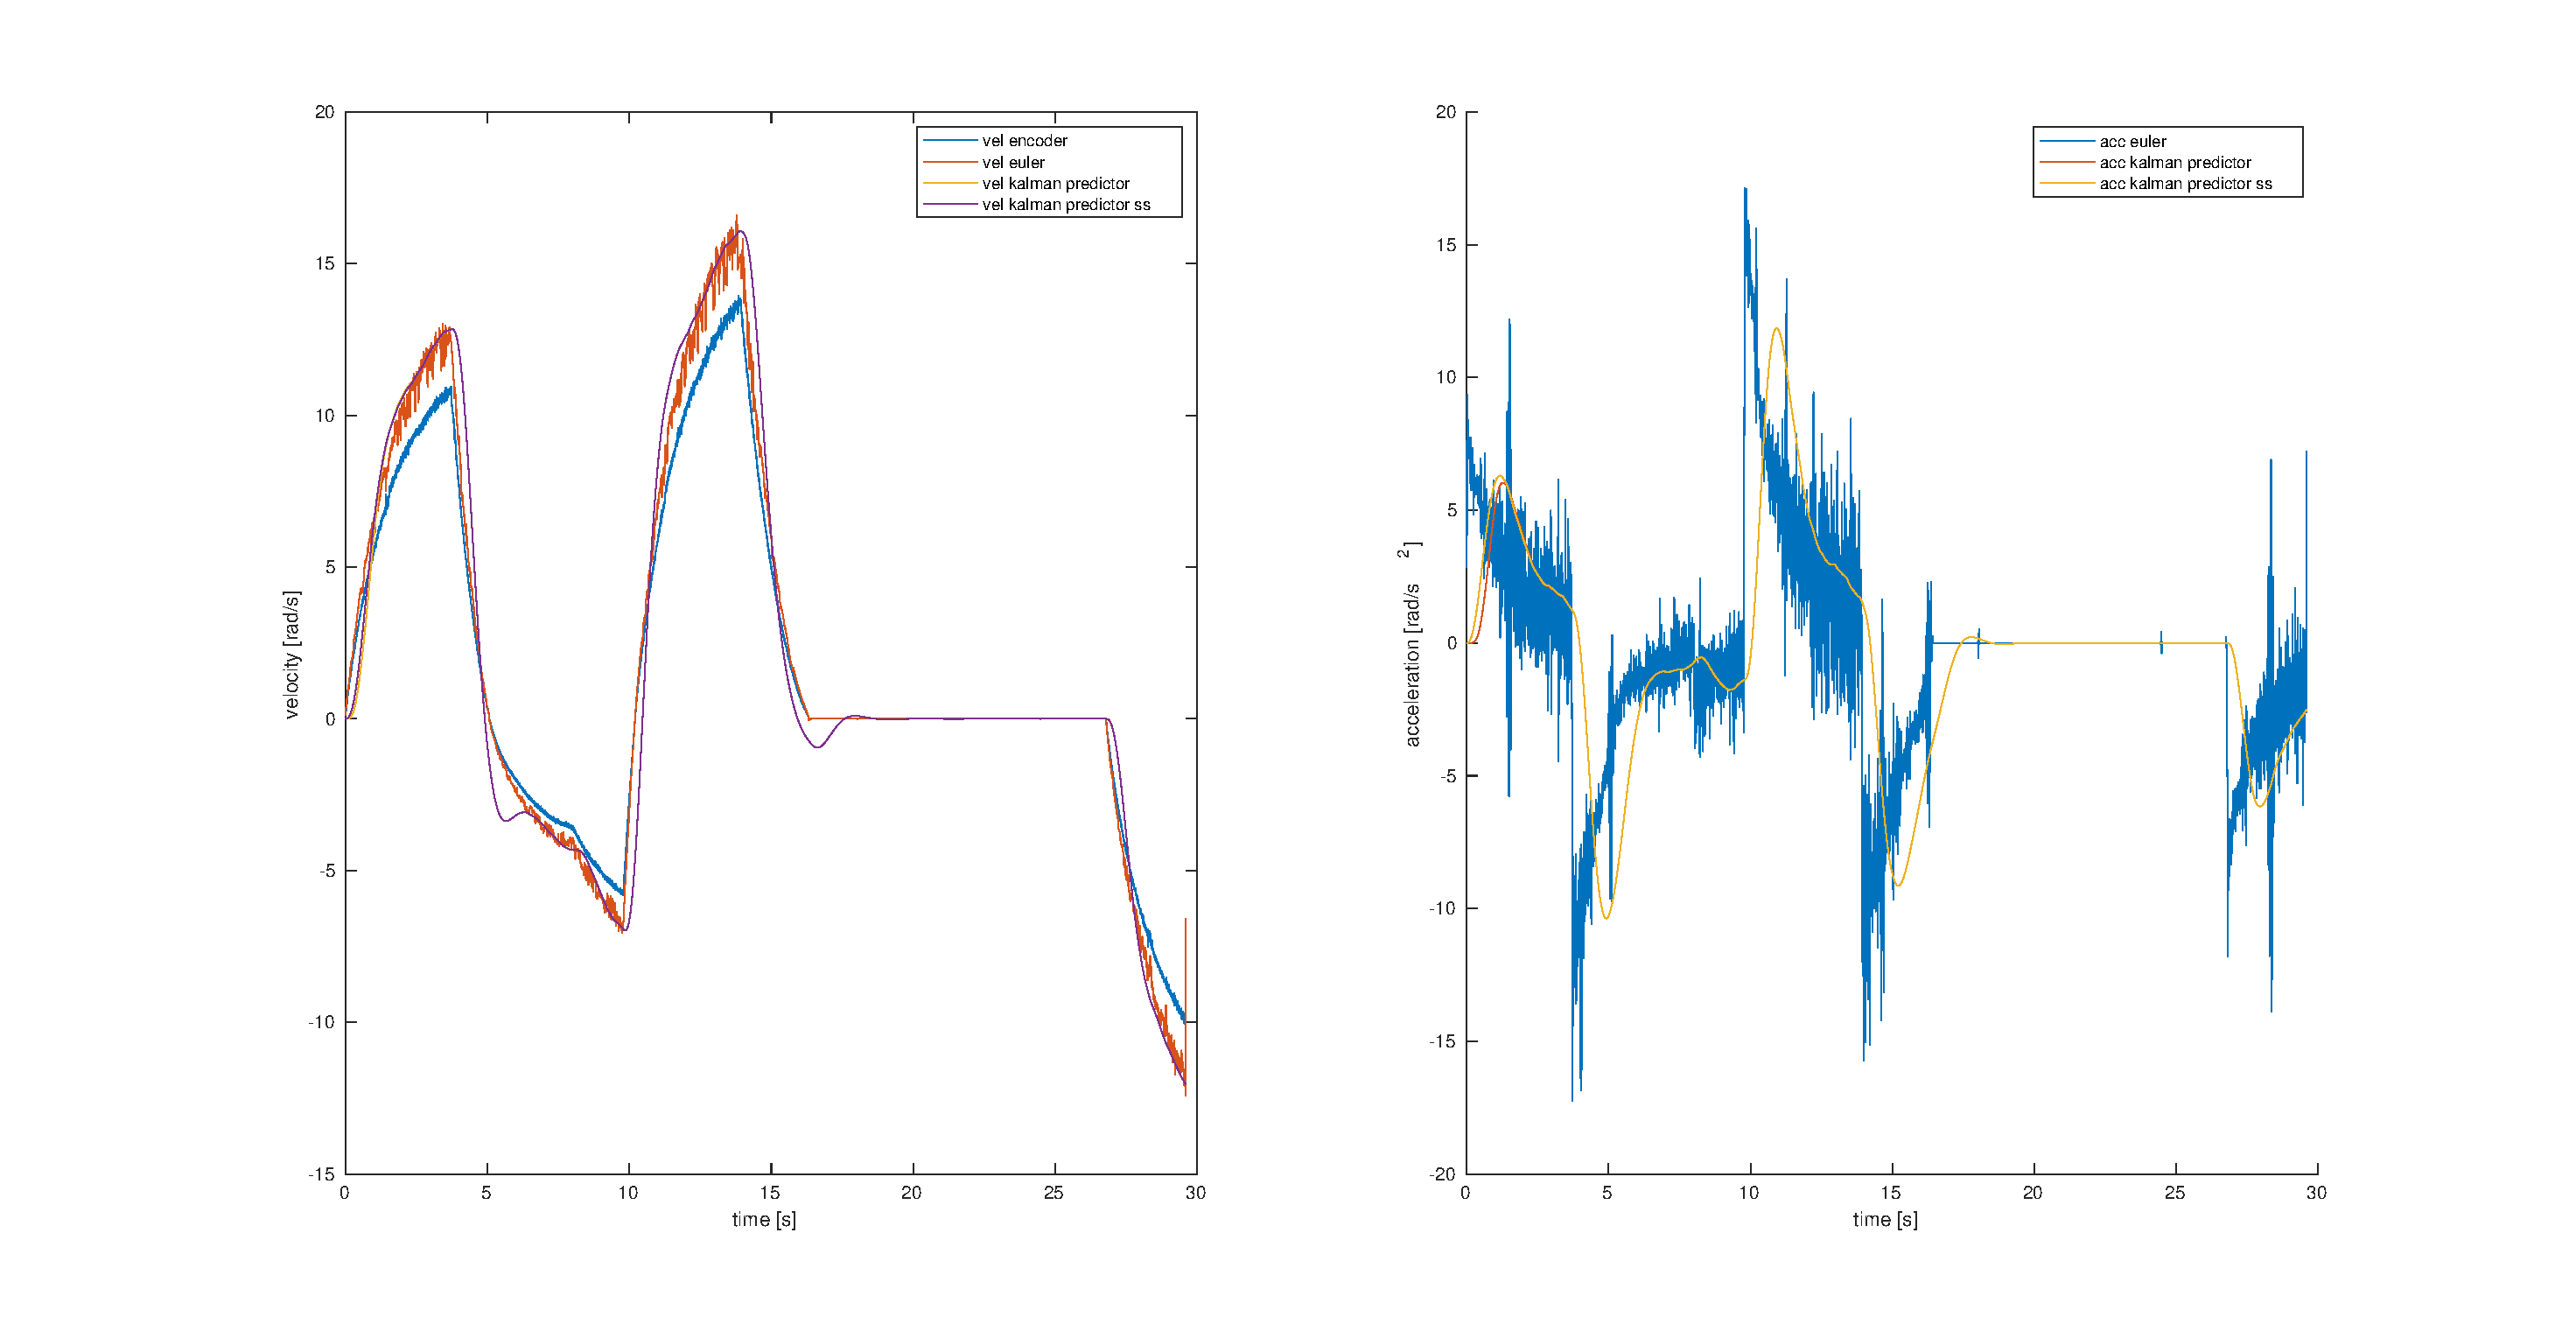
\includegraphics[scale=0.5]{images/kalman_predictor.eps}
    \end{center}
    \caption{Velocities and accelerations estimations using Kalman predictor, Kalman predictor in steady state conditions and euler approximations with 5Hz low pass filter. As it is visible at the beginning the Kalman predictor is different from the steady state version.}
    \label{fig:kalman_predictor}
\end{figure}

In Fig \ref{fig:kalman_smoother} the use of the kalman smoother is reported. Informally, thanks to both forward (Kalman filter) and backward (smoothing) steps the Kalman smoother in general performs a better estimation for the given dataset.
\begin{figure}[H]
    \begin{center}
        \hspace*{-4.6cm}
        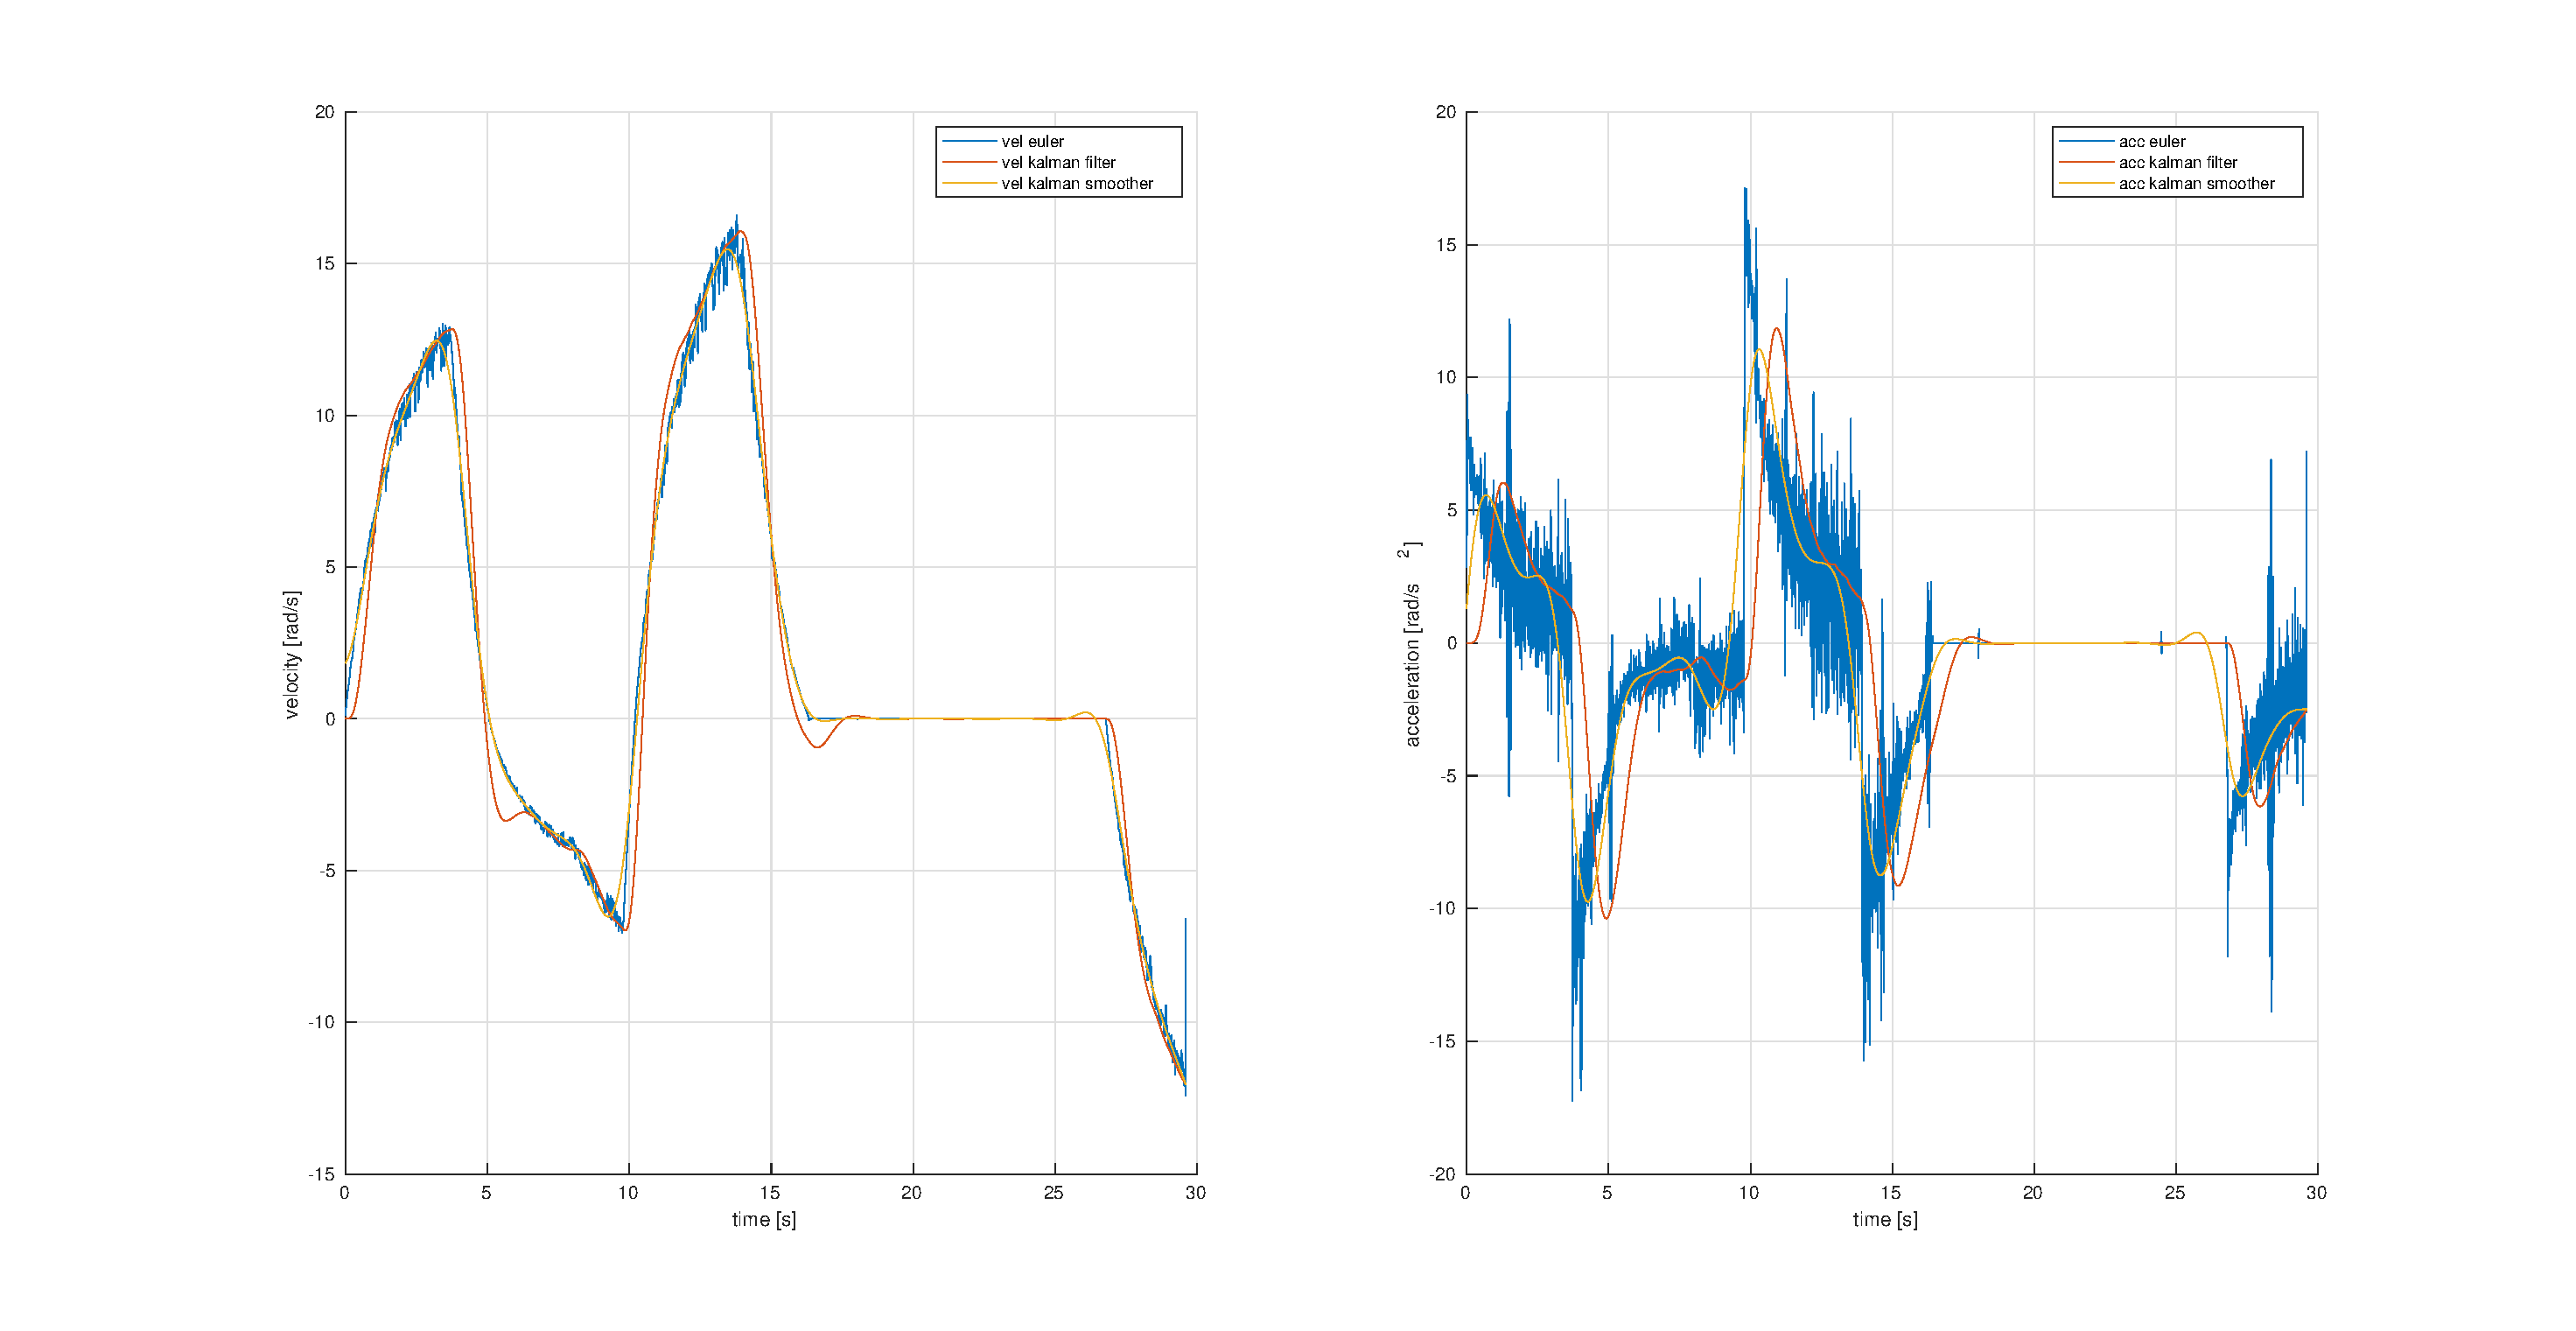
\includegraphics[scale=0.5]{images/kalman_smoother.eps}
    \end{center}
    \caption{Velocities and accelerations estimations using Kalman filter and Kalman Smoother}
    \label{fig:kalman_smoother}
\end{figure}
\section{Least Square, RLS and Adaptive Estimation}
The aim of this section is to present three techniques to solve a gray-box indentification problem meaning that the class of the model is known but the specific parameters are unknown. If we consider a linear model:
\[
    y = x\beta \qquad \textit{for example a DC motor} \qquad V(t) = \begin{bmatrix}
        \dot{w}(t) & w(t) 
    \end{bmatrix} \begin{bmatrix}
        \tau/k \\ 1/k
    \end{bmatrix}
\]
the aim is to find the prediction:
\[
    \hat{y} = x \hat{\beta}
\]
where $\hat{\beta} \in \mathbb{R}^m$ is the matrix of coefficients that we have to determine.

\bigskip
\noindent The following methods are reported:
\begin{itemize}
    \item \textbf{Least square solution} $\hat{\beta} = (X^TX)^{-1}X^TY$ if $X^TX$ is non-singular
    \item \textbf{Adaptive algorithm} $\hat{\beta}(k) = \hat{\beta}(k-1) + T_sgx^T(k)e(k)$ with $g > 0$. Basically we are moving in the opposite direction of the gradient of the minimized square error.
    \item \textbf{Recursive Least square} by solving the causal formulation:
\end{itemize}
\[
    \begin{cases}
        e(k) = y_k -x_k\hat{\beta}(k-1) \\
        P(k) = \frac{1}{\lambda} \left ( P(k-1) - \frac{P(k-1)x_k^Tx_kP(k-1)}{\lambda + x_kP(k-1)x_k^T}\right) \\ 
        K(k) = P(k)x_k^T \\
        \hat{\beta}(k) = \hat{\beta}(k-1) + K(k)e(k) 
    \end{cases}
\]
where $0 < \lambda \leq 1 $ is called forgetting factor. The results obtained by the models are close to $k = 15.226487$ and $\tau = 1.212946$.

\begin{figure}[H]
    \begin{center}
        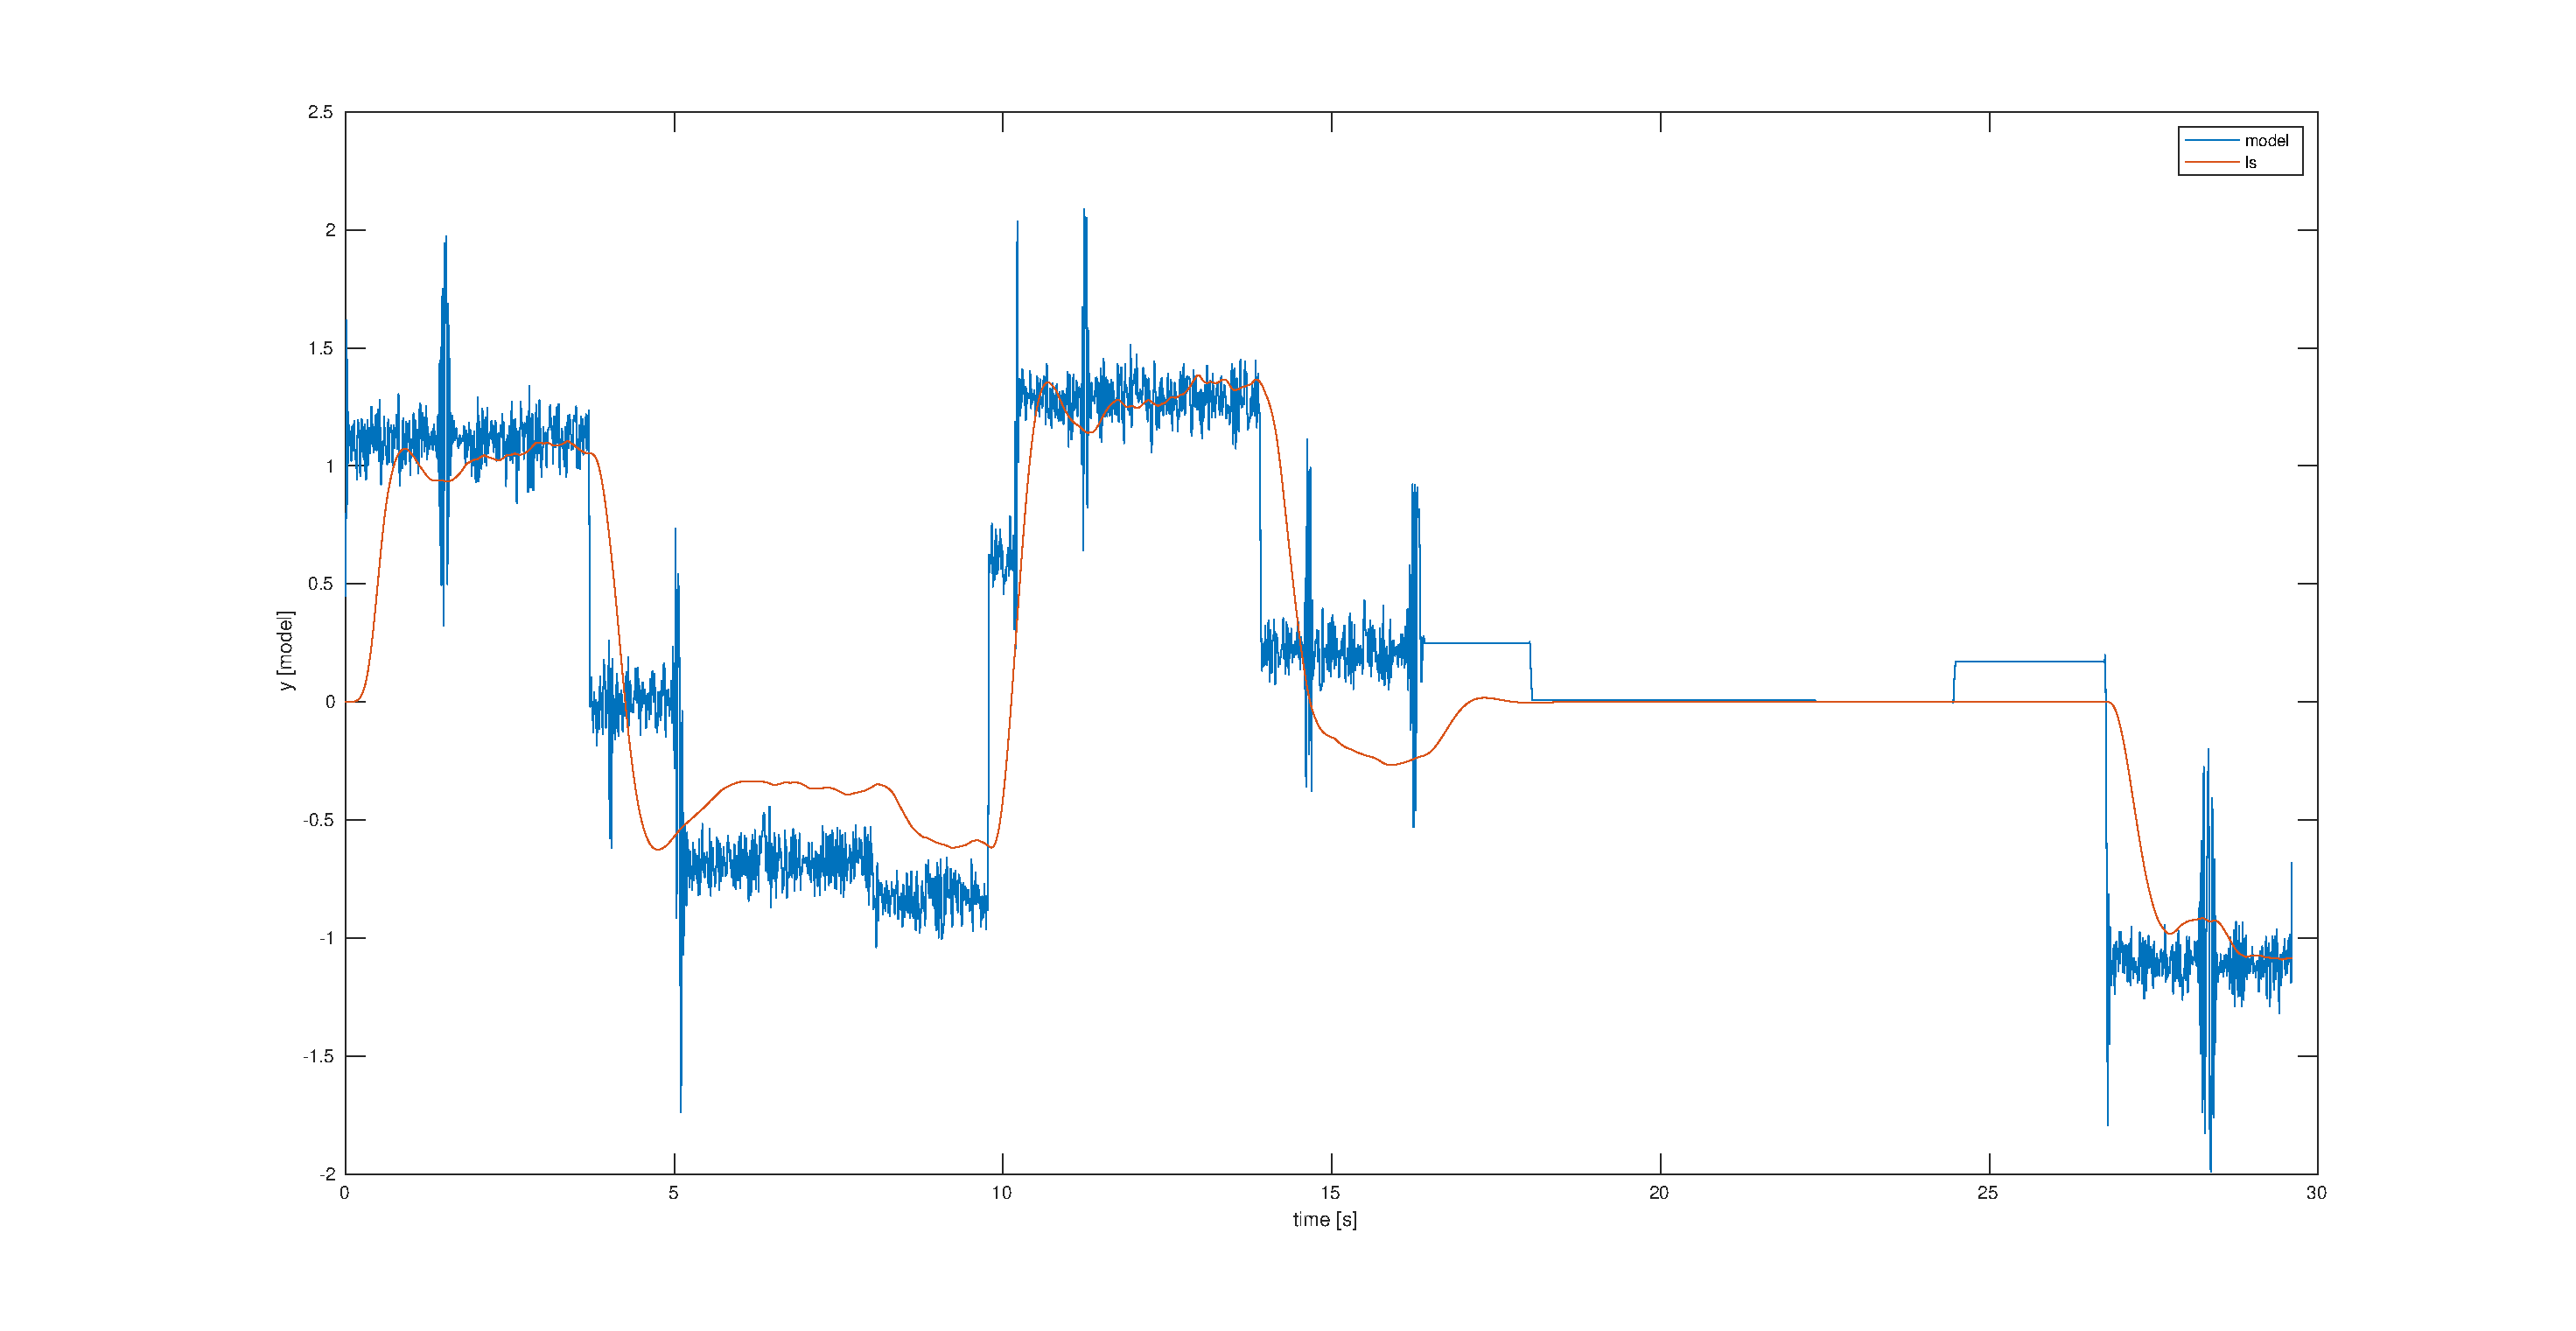
\includegraphics[scale=0.3]{images/ls.eps}
    \end{center}
    \caption{Least square estimation of the DC model of the motor}
    \label{fig:ls}
\end{figure}

\begin{figure}[H]
    \begin{center}
        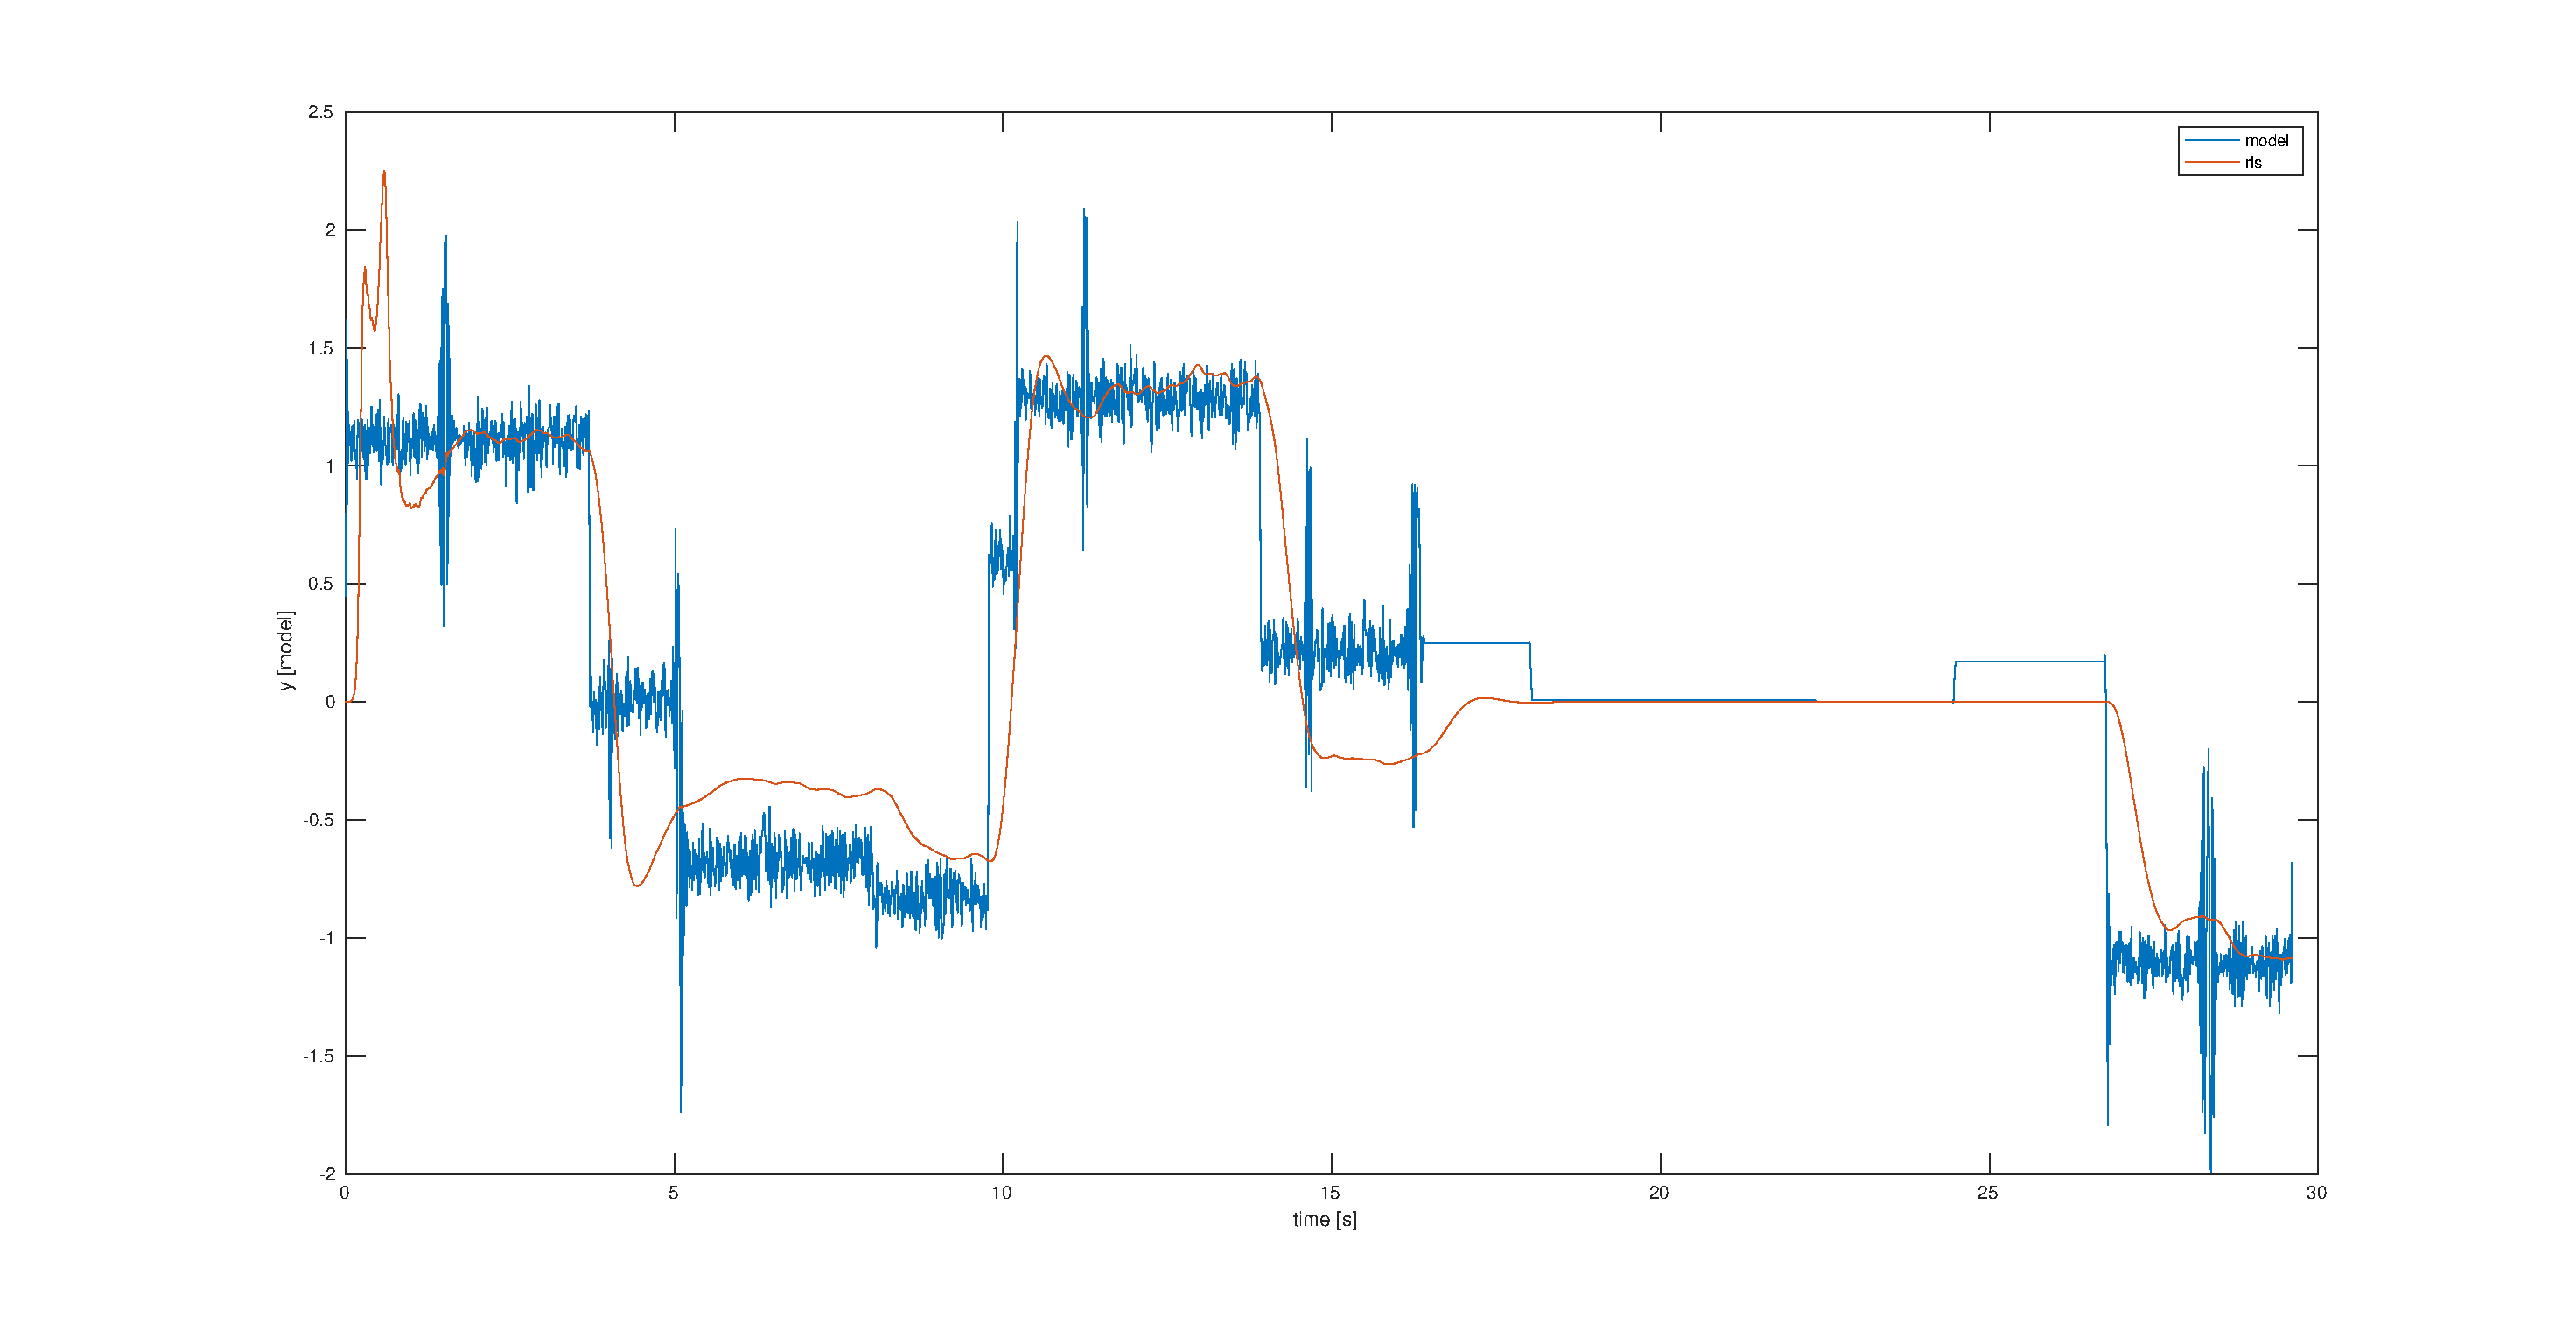
\includegraphics[scale=0.3]{images/rls.eps}
    \end{center}
    \caption{Recursive least square estimation of the DC model of the motor}
    \label{fig:rls}
\end{figure}

\begin{figure}[H]
    \begin{center}
        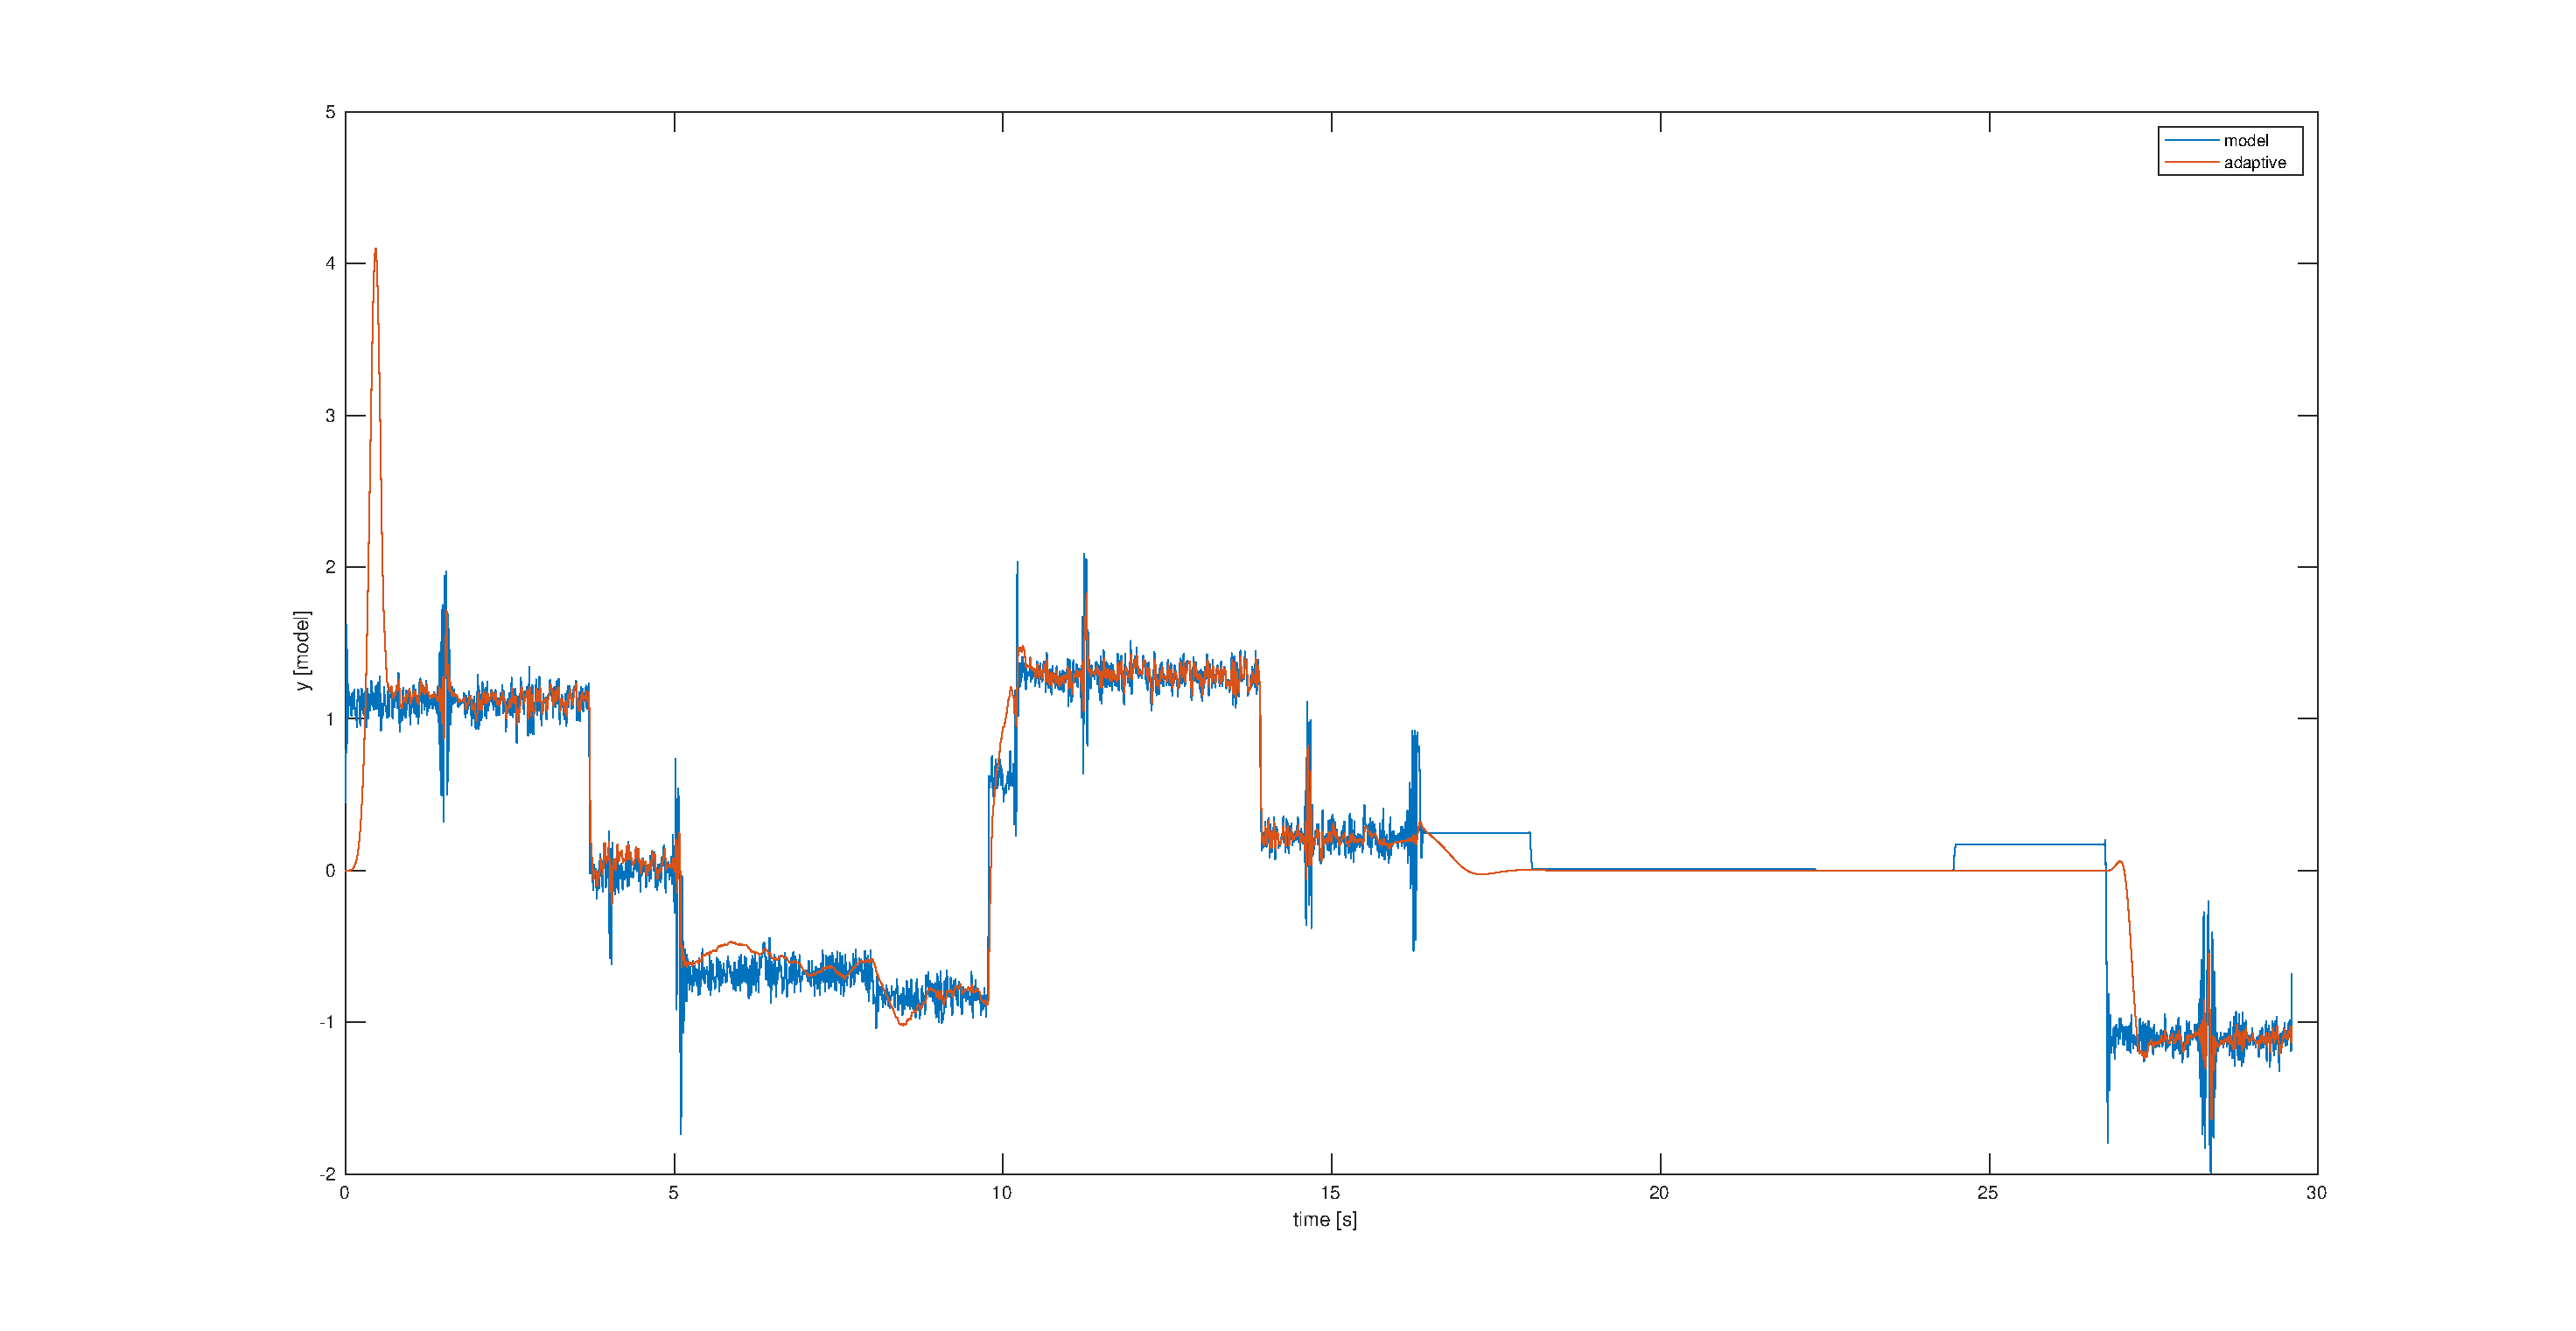
\includegraphics[scale=0.3]{images/adaptive.eps}
    \end{center}
    \caption{Adaptive estimation of the DC model of the motor with $g = 0.54$}
    \label{fig:adaptive}
\end{figure}

\begin{figure}[H]
    \begin{center}
        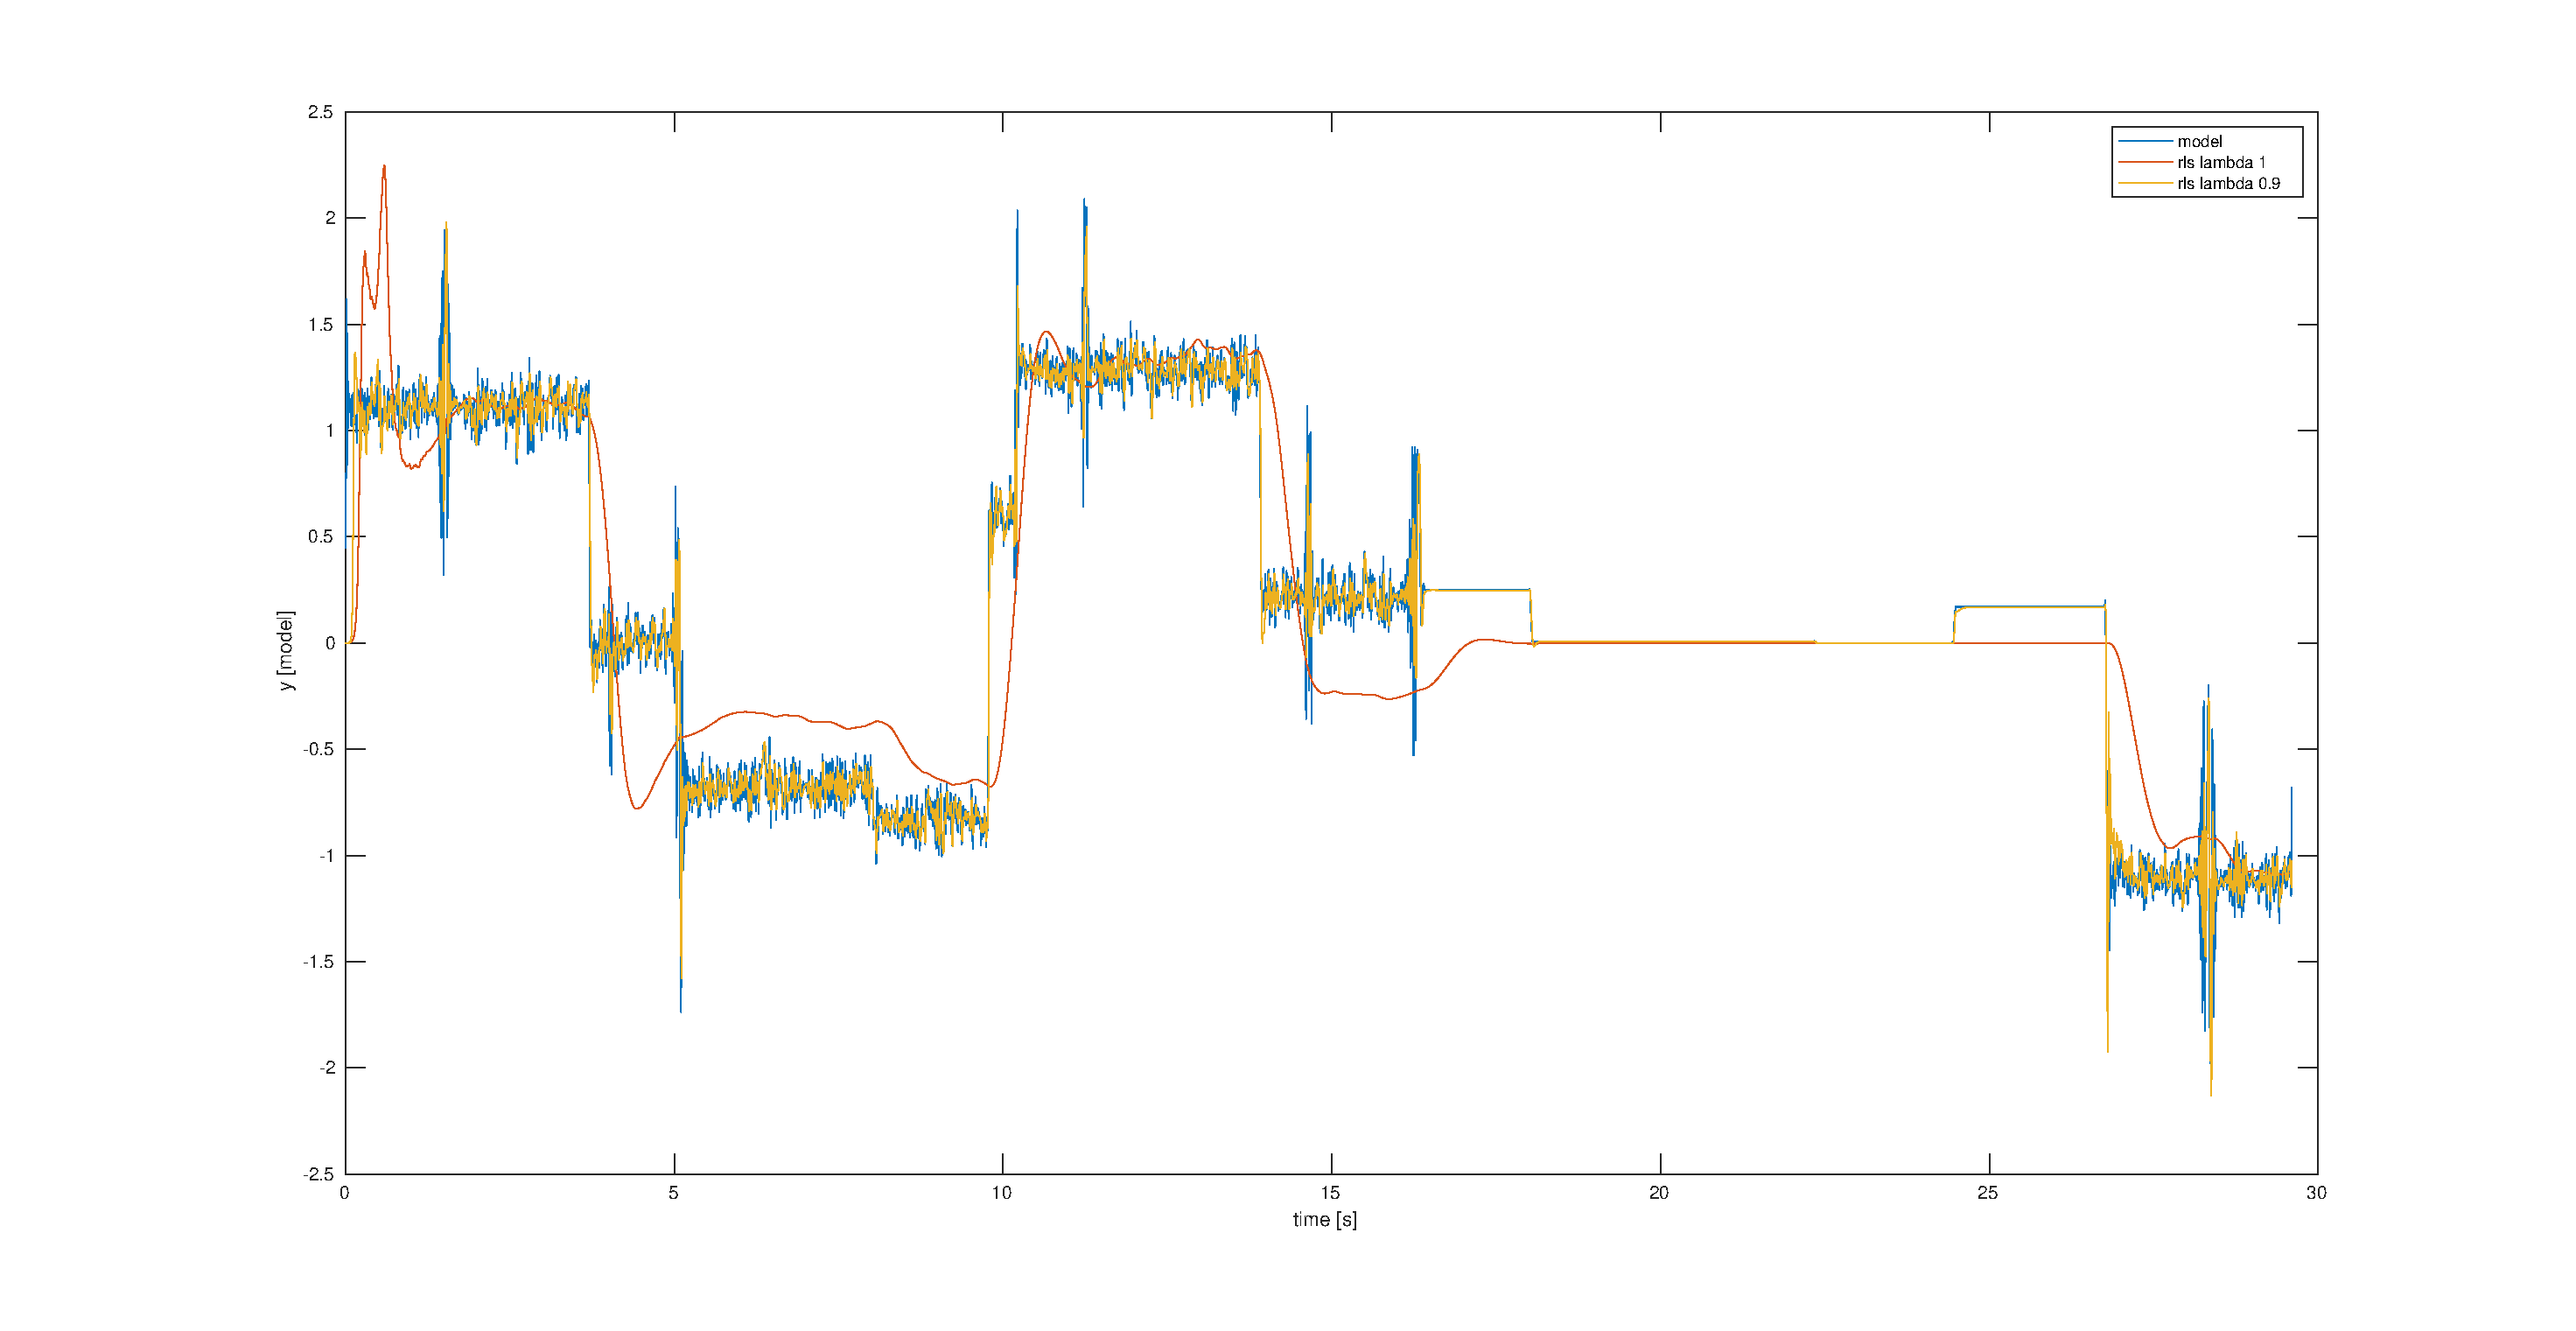
\includegraphics[scale=0.3]{images/rls_forget.eps}
    \end{center}
    \caption{Recursive least square with forgetting factor of the DC model of the motor}
    \label{fig:rls_f}
\end{figure}

\section{Scattering based bilateral teleoperation architecture}
The core ideas in this architecture were described by Niemeyer and Slotine in Stable Adaptive Teleoperation (1991). The paper was \begin{quote}
    a preliminary study on how the existence of time-delays affects the application of advanced control schemes to effective force-reflecting telerobotic systems.
\end{quote}

The fundamental ideas are developed in the context of passivity formalism which
\begin{quote}
    represents a mathematical description of the intuitive physical concepts of power and energy. It provides a simple and robust tool to analyze the stability of a nonlinear system while maintaining global stability properties.
\end{quote}
A system is said passive if:
\[
    P = x^Ty = \frac{dE}{dt} + P_{diss}
\]
and it is also true that:
\[
    \int_{0}^{t} P \,d\tau = \int_{0}^{t} x^Ty \,d\tau = E(t) - E(0) + \int_{0}^{t} P_{diss} \,d\tau \geq -E(0) = \text{constant}
\]

\noindent The interesting properties of passivity formulations are its closure properties via feedback or parallel configuration. Moreover 

\begin{quote}
    the use of passivity is a sufficient condition for the stability of the system coupled to a passive environment with a bounded operator input energy.
\end{quote}

\noindent The wave variable formulation, formally treated in scattering theory, is introduced. In this context a system is passive if the energy provided by the output waves is limited to the energy received via input waves
\[
    \int_{0}^{t} \frac{1}{2}v^Tv \,d\tau \leq \int_{0}^{t} \frac{1}{2}u^Tu \,d\tau 
\]
The transformations used to map $(\dot{x},F)$ into $(u,v)$ are:
\[
    u_l = \frac{1}{\sqrt{2b}}(F_l + b \dot{x_l}) \qquad u_r = \frac{1}{\sqrt{2b}}(F_r - b \dot{x_r}) 
\]

\[
    v_l = \frac{1}{\sqrt{2b}}(F_l - b \dot{x_l}) \qquad v_r = \frac{1}{\sqrt{2b}}(F_r + b \dot{x_r}) 
\]
they can be used to extract the desired configurations based on the signal provided such as forces or velocities.

\newpage
\subsection{Scattering based Force-Position}

The idea of the scattering based FP is to use the master velocity as a velocity reference for the slave side and the interaction force with the environment as a reference for the master side. In this scenario the scattering based architecture Position-Force was evaluated with a delay of 10 time steps in the communication channel. The environment used is $B_e = 10$ and $K_e = 200$. 

\[
    \begin{cases}
    u_l=\sqrt{2b}\dot{x}_l+v_l\\
    F_l=b\dot{x}_l+\sqrt{2b}v_l
    \end{cases}
    \begin{cases}
    u_r=\sqrt{\frac{2}{b}}F_r-v_r\\
    \dot{x}_r=-\frac{1}{b}(F_r-\sqrt{2b}v_r)
    \end{cases}
\]

\bigskip
In Fig \ref{fig:scat_pf_free} the free motion case is reported. As it is visible the system is stable and there is a minimal delay in the position compared to reference $x_d$.

\begin{figure}[H]
    \begin{center}
        \hspace*{-4.5cm}
        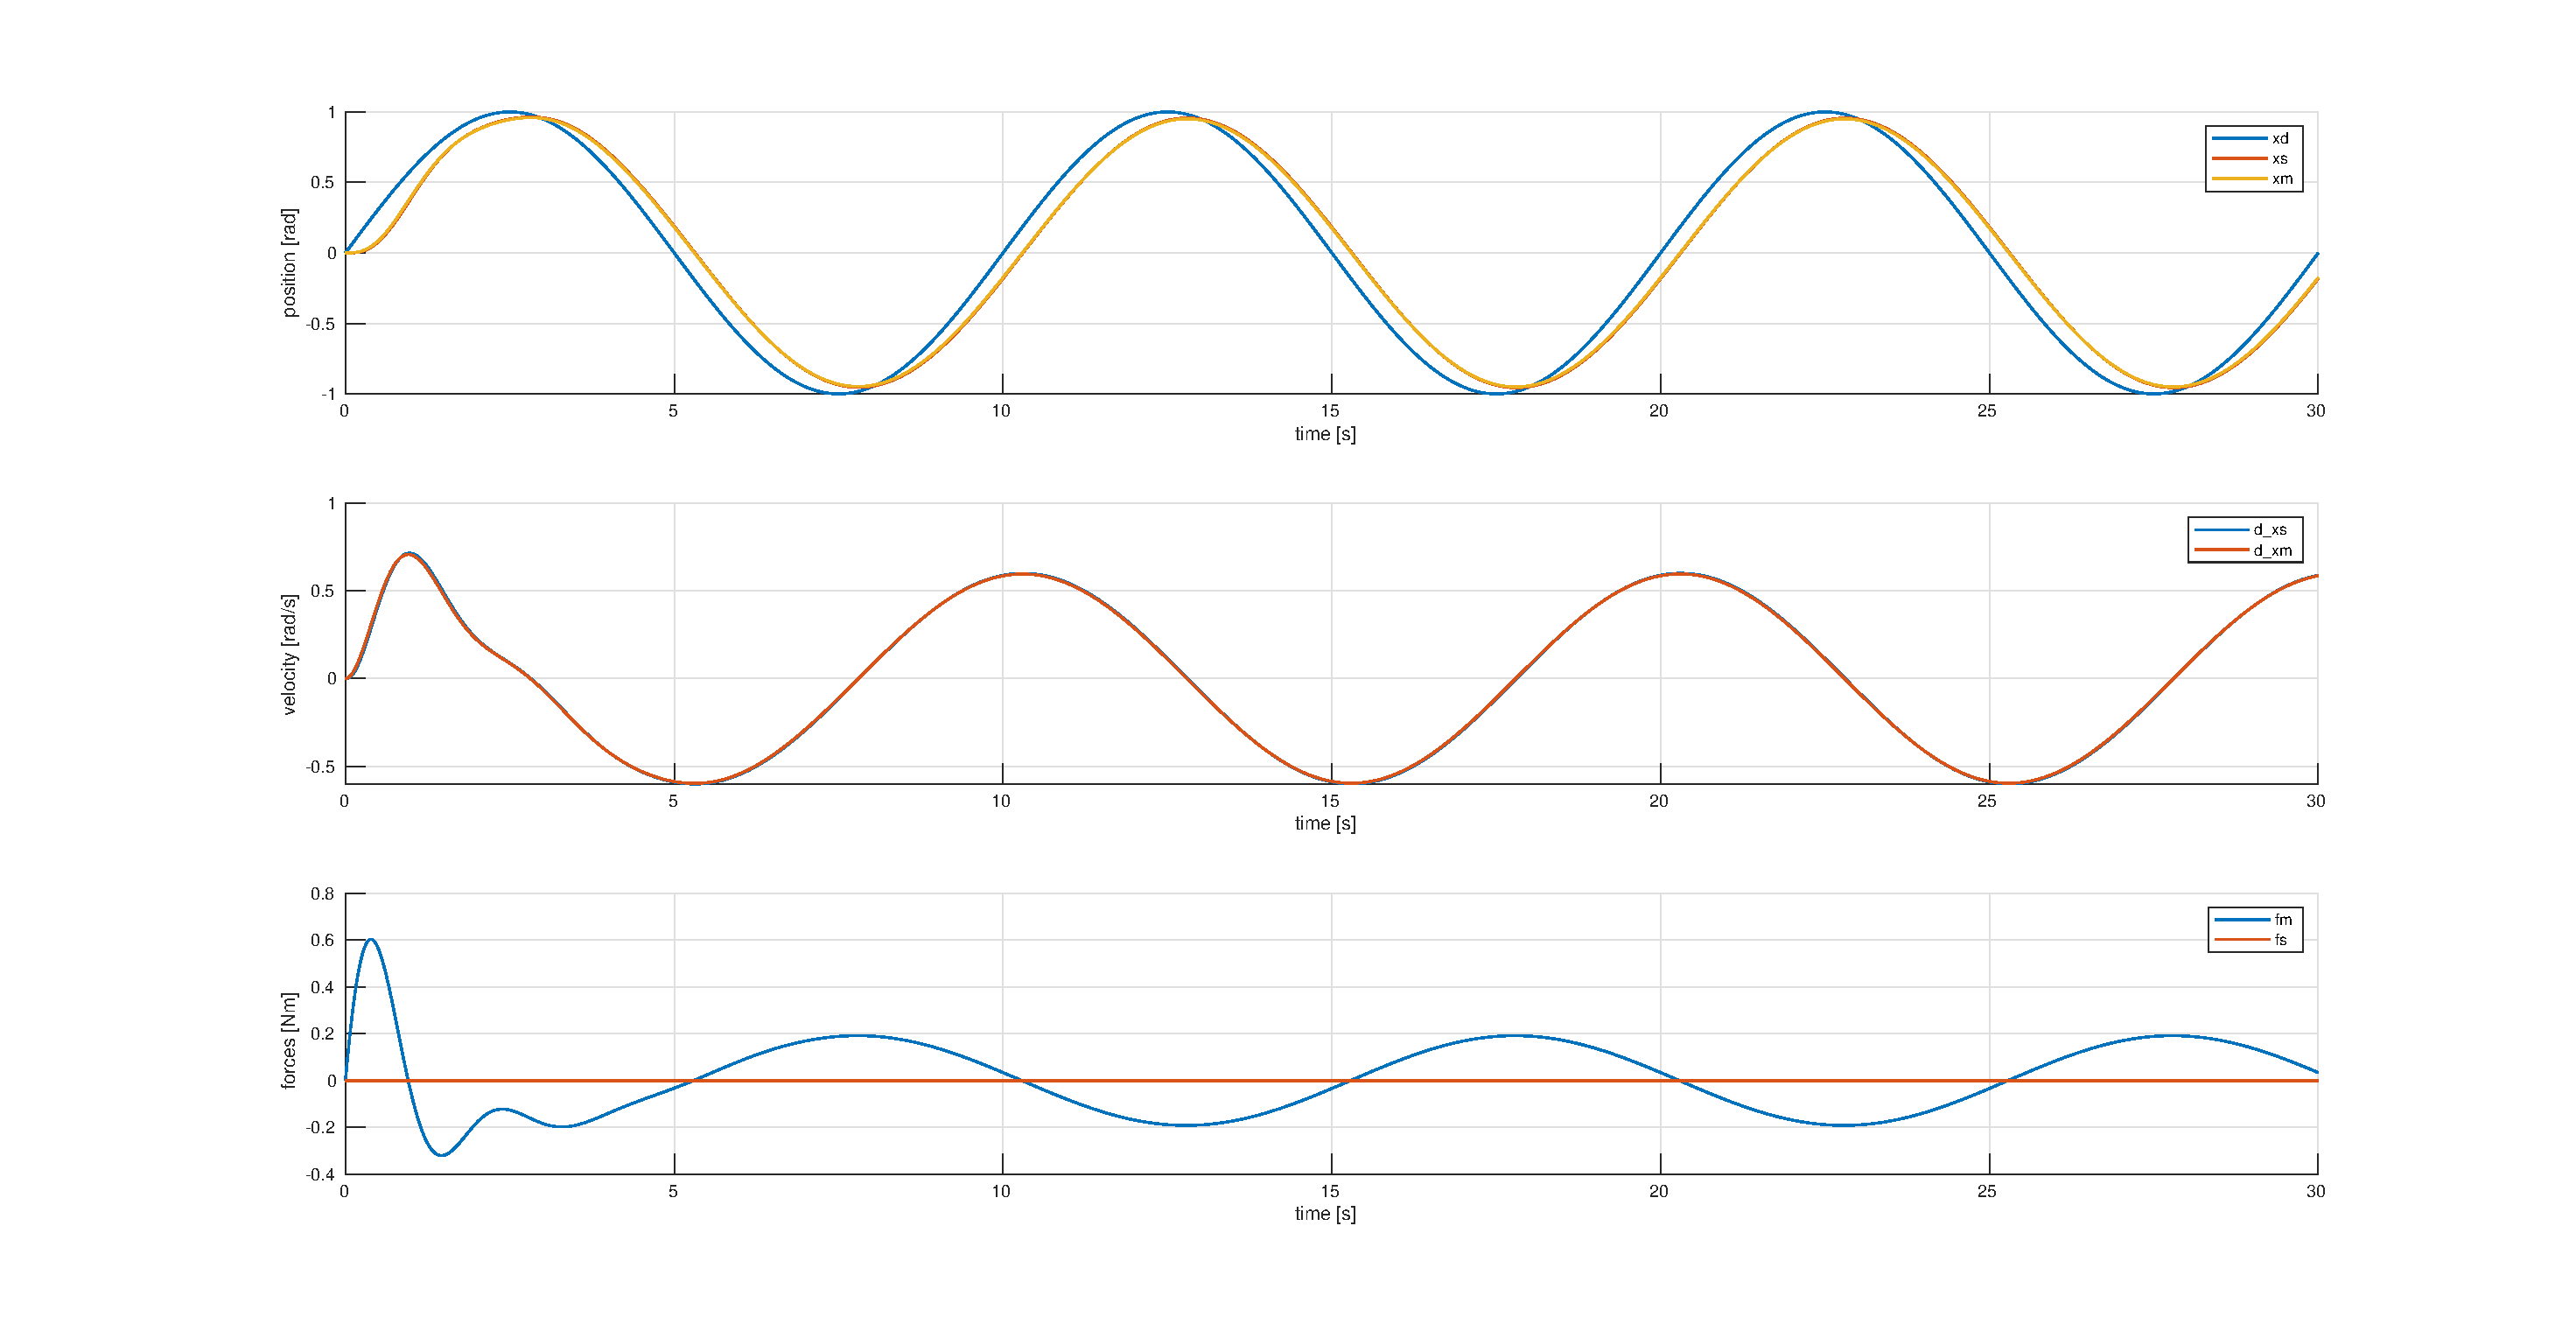
\includegraphics[scale=0.5]{images/scat_pf_free.eps}
    \end{center}
    \caption{Scattering based FP in free motion, a low pass filter is introduced in the scattering formulation to correct numerical errors at 100Hz}
    \label{fig:scat_pf_free}
\end{figure}

\newpage
In Fig \ref{fig:scat_pf_contact} the contact case is reported. As it is visible there is some "noise" in the velocities and forces plots: the low pass filter implemented in the communication channel can leverage this problem by decreasing the cut-off frequency. A cut-off frequency of 10 Hz was used to produce the figure.

\begin{figure}[H]
    \begin{center}
        \hspace*{-4.5cm}
        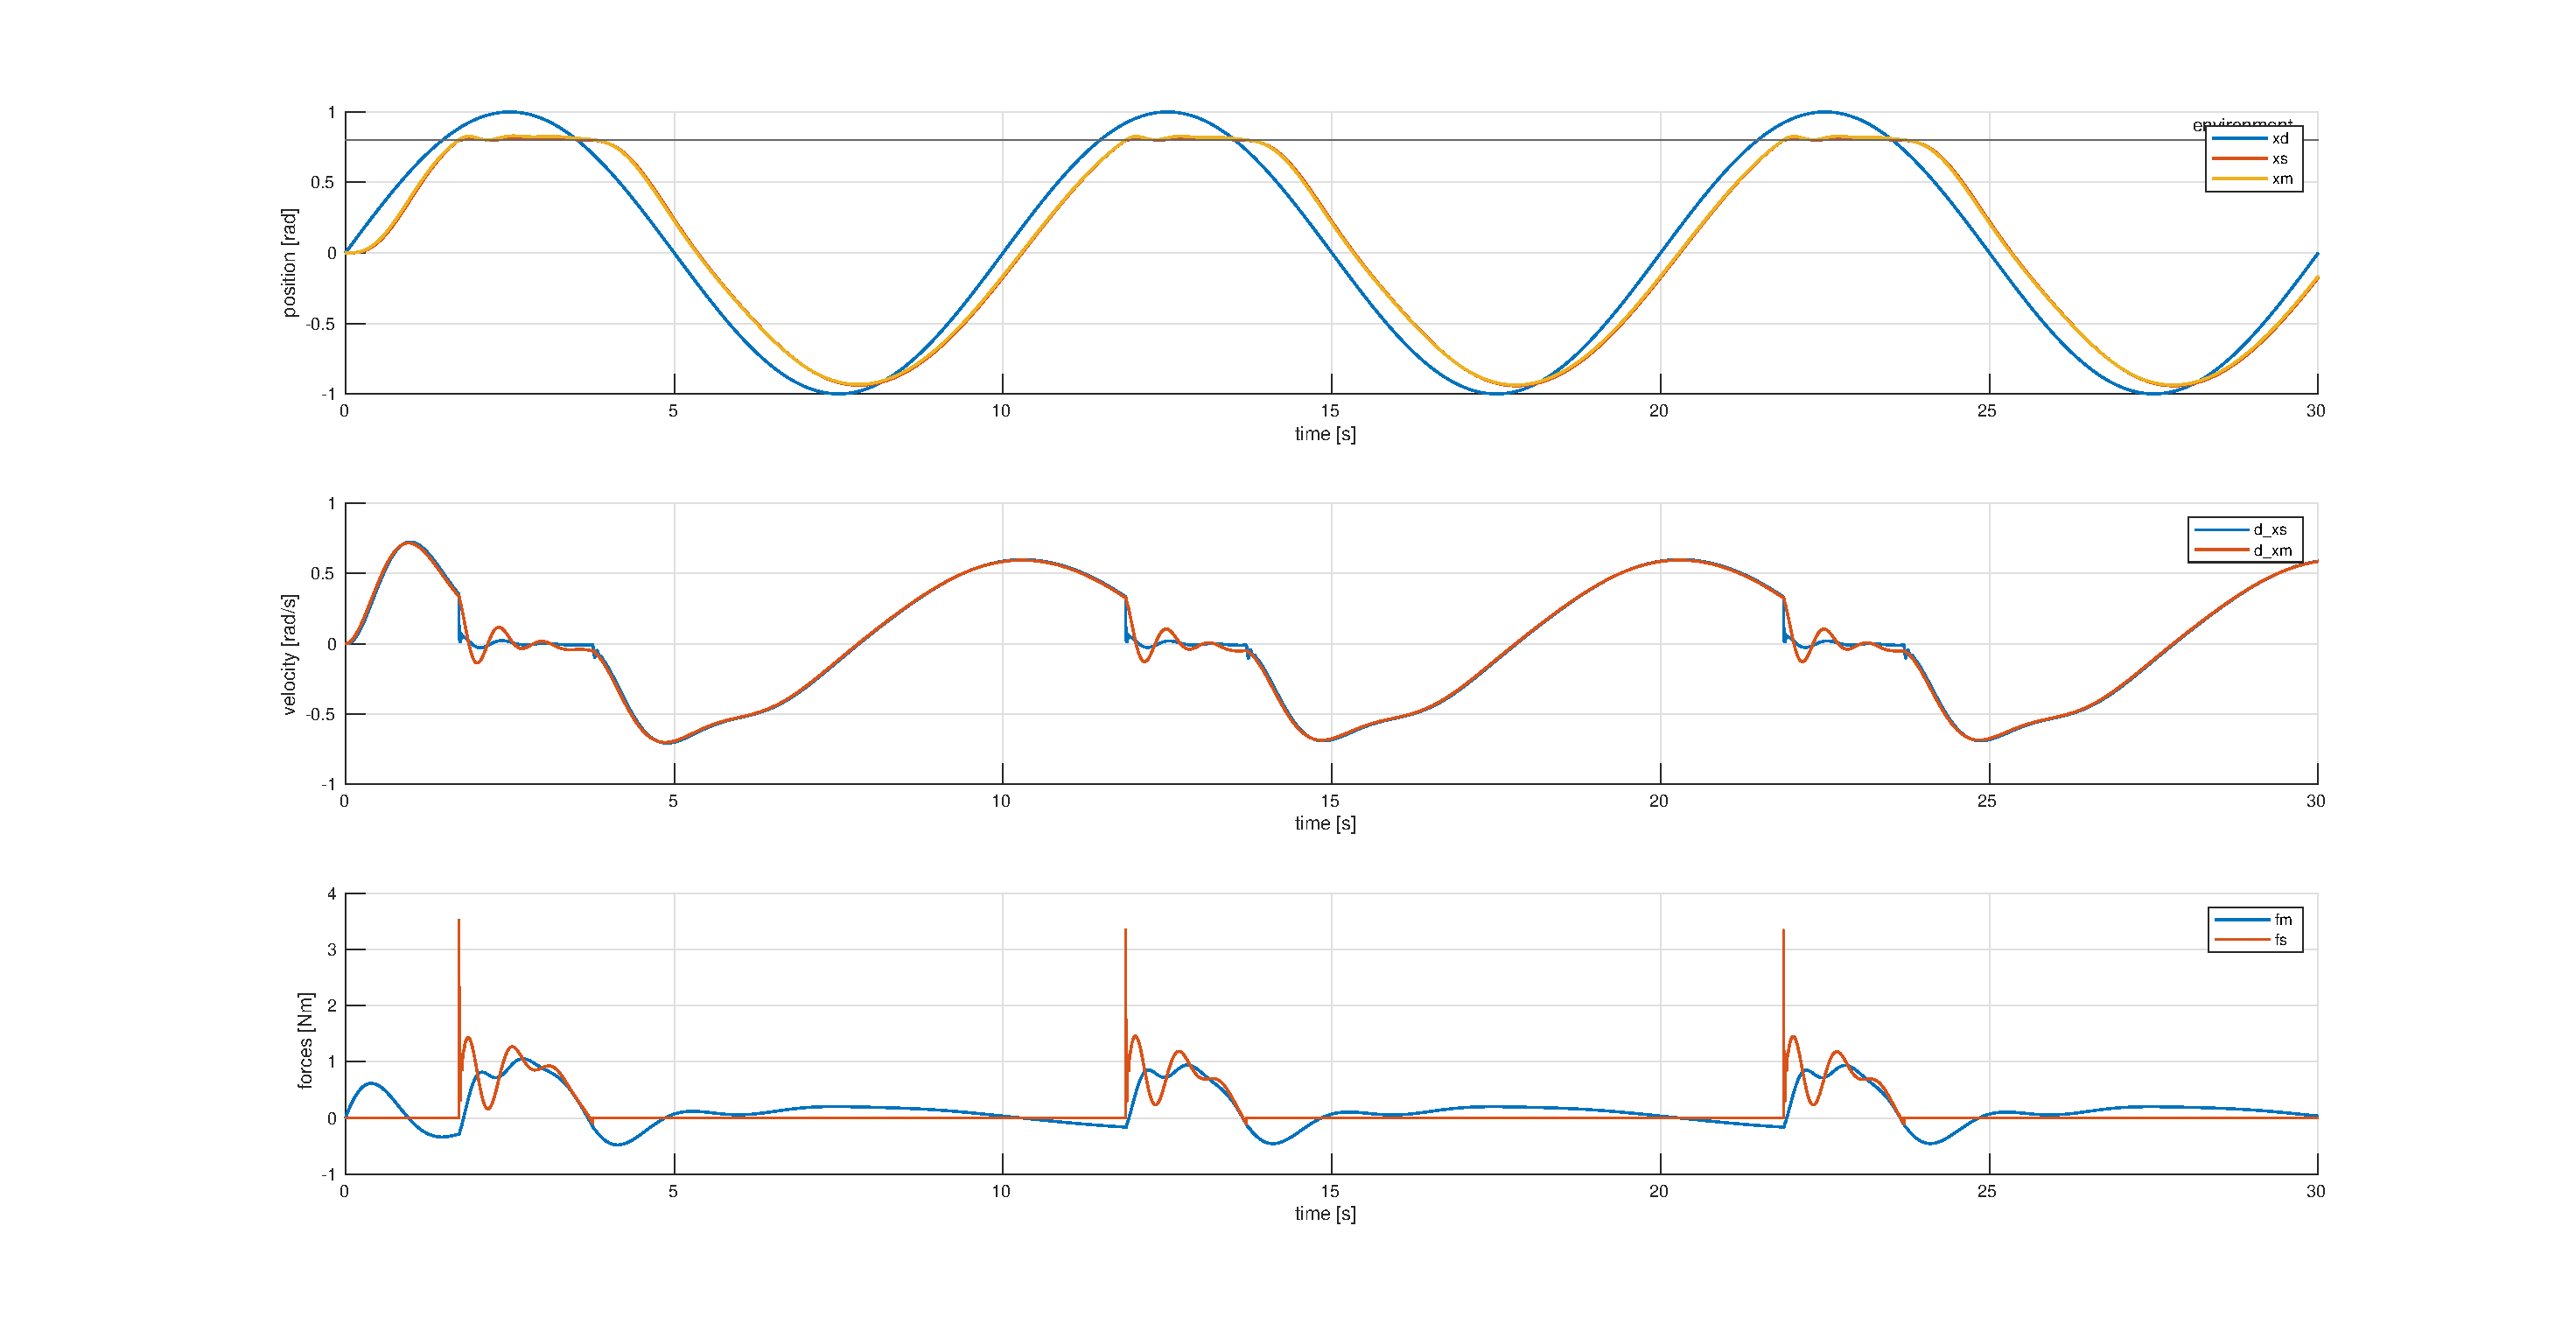
\includegraphics[scale=0.5]{images/scat_pf_contact.eps}
    \end{center}
    \caption{Scattering based FP in contact with a stiff environment at 0.8}
    \label{fig:scat_pf_contact}
\end{figure}

In Fig \ref{fig:scat_pf_contact_kalman} some noise measurements are added, both on velocities and forces, to the architecture as well as a kalman filter to get position and velocity estimations both at master and slave side. Finally the internal low pass filter in the communication channel was introduced with a cut-off frequency of 10Hz. As it is visible both the velocities and the forces are affected by noise.

\begin{figure}[H]
    \begin{center}
        \hspace*{-4.5cm}
        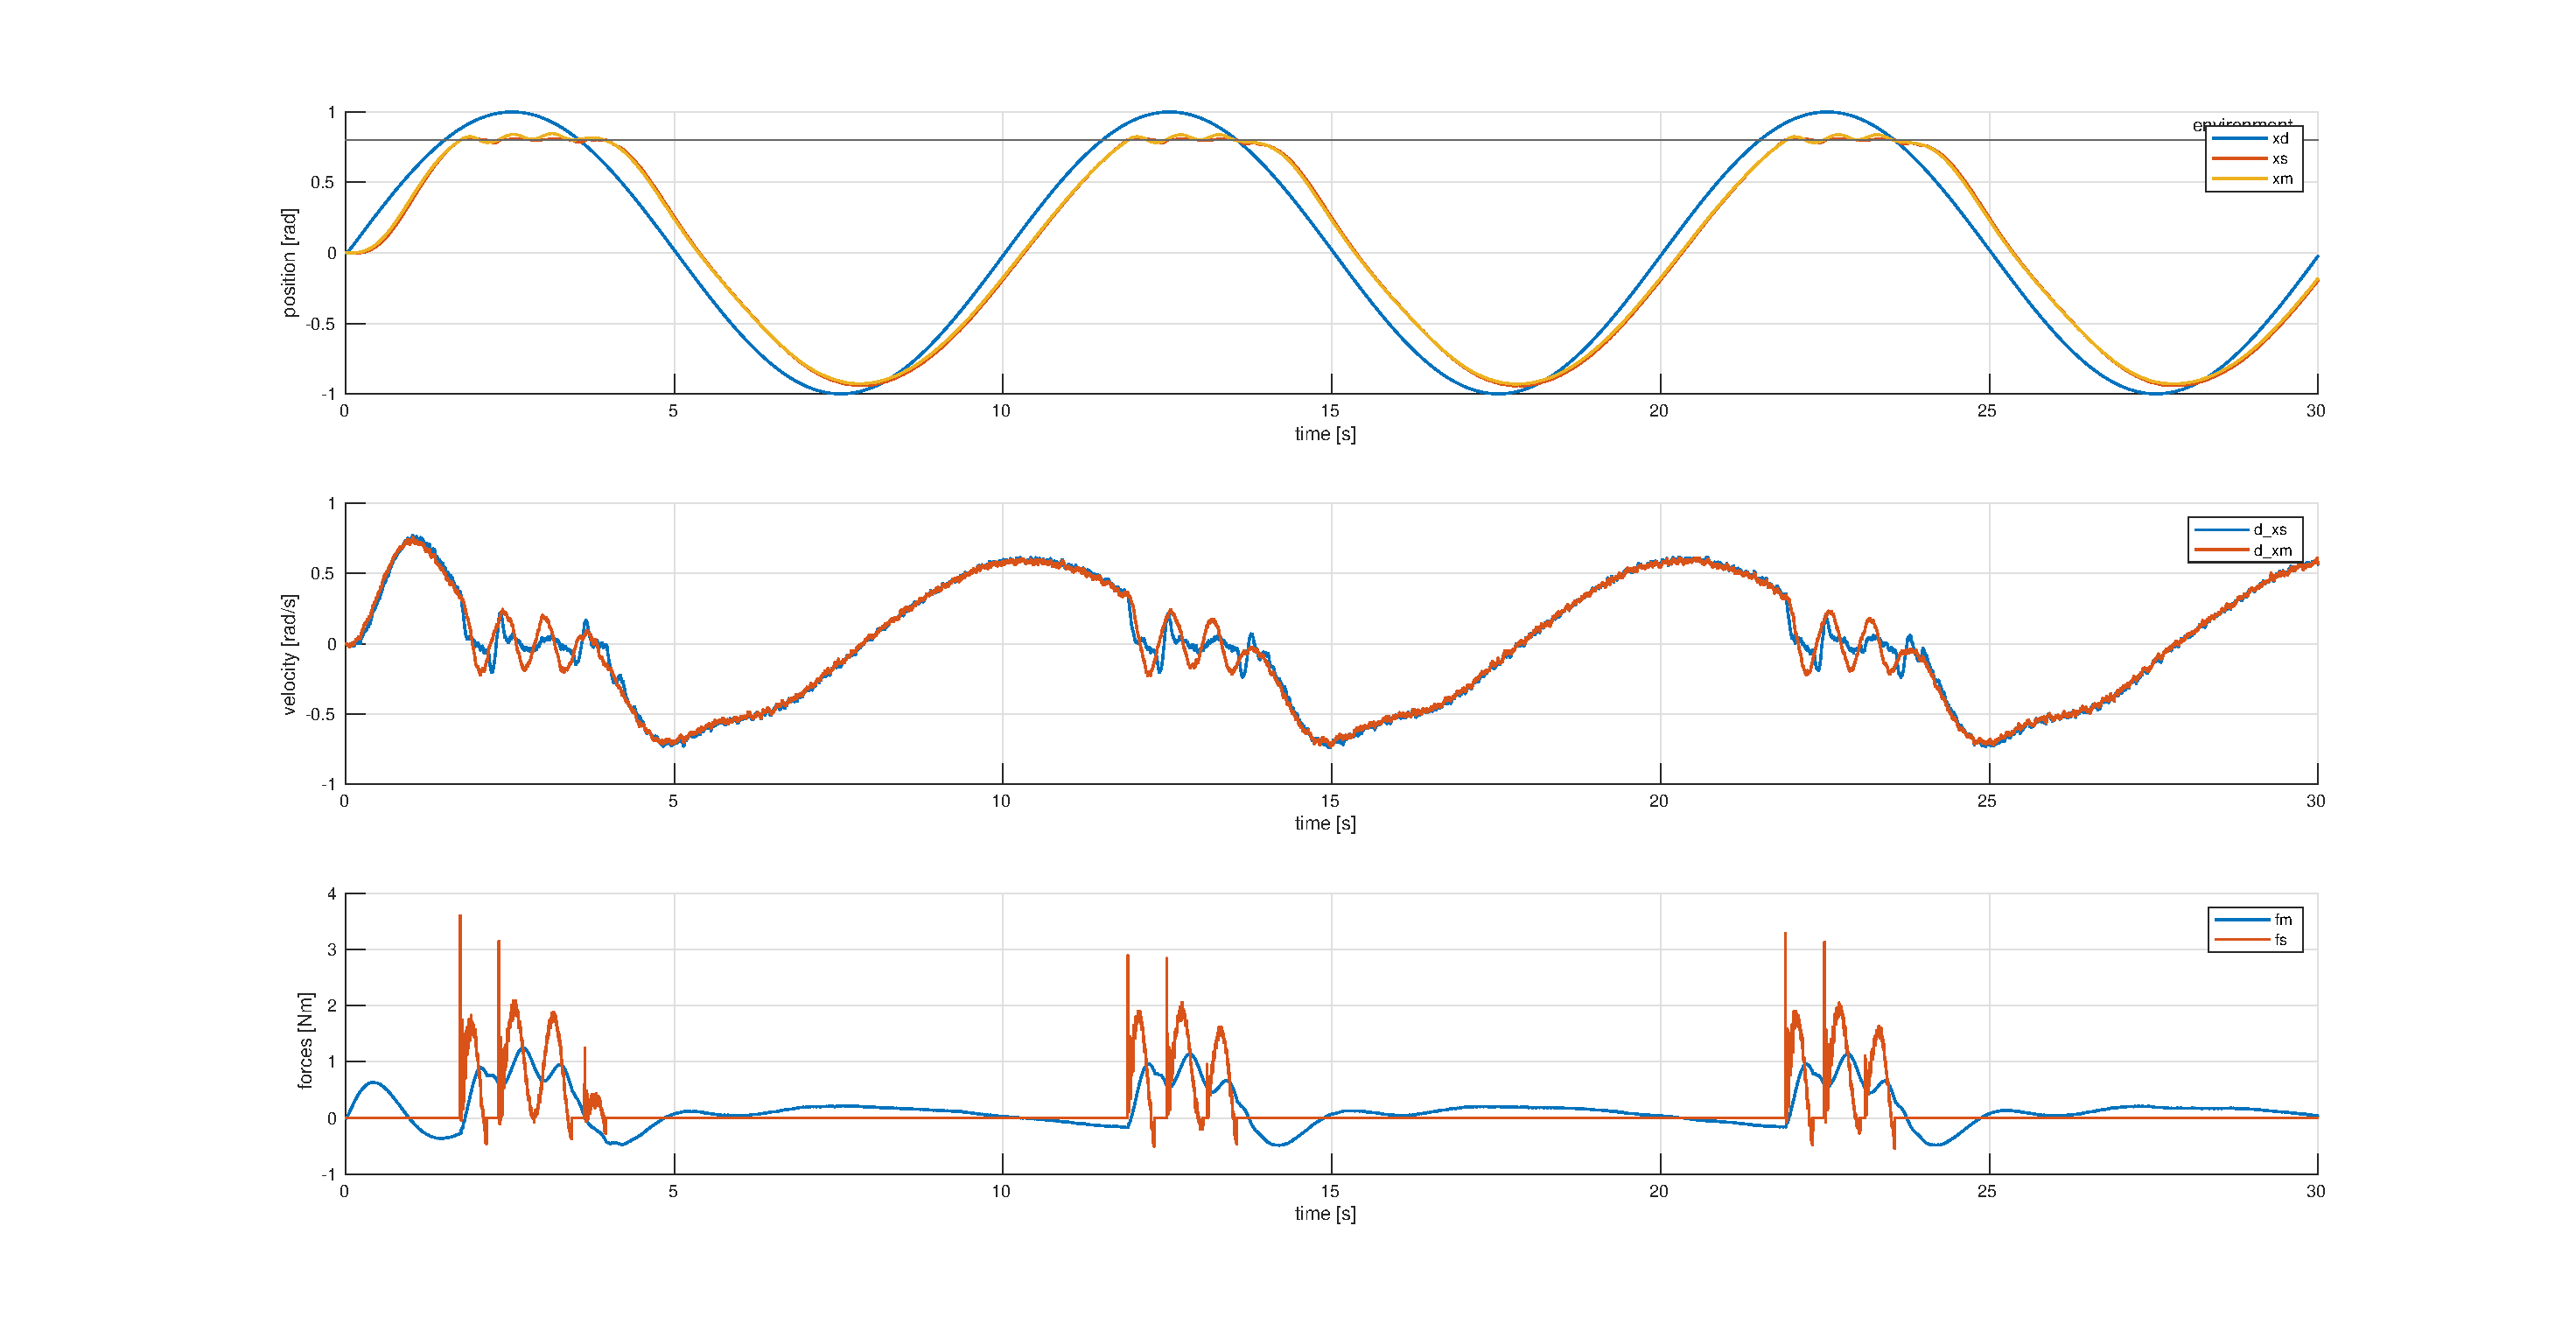
\includegraphics[scale=0.5]{images/scatt_pf_contact_kalman.eps}
    \end{center}
    \caption{Scattering based FP with noisy measurements and kalman filters in contact with a stiff environment at 0.8}
    \label{fig:scat_pf_contact_kalman}
\end{figure}

In all the previous plots the scattering variables were not considered. For simplicity they are reported only once in a contact case in Fig \ref{fig:scat_var}. As it is visible forces and velocities should match according to the scattering formulation. There numerical problems during the immediate contact as it is clearly visible and it can be corrected by adjusting the low pass filter.
\begin{figure}[H]
    \begin{center}
        \hspace*{-4.5cm}
        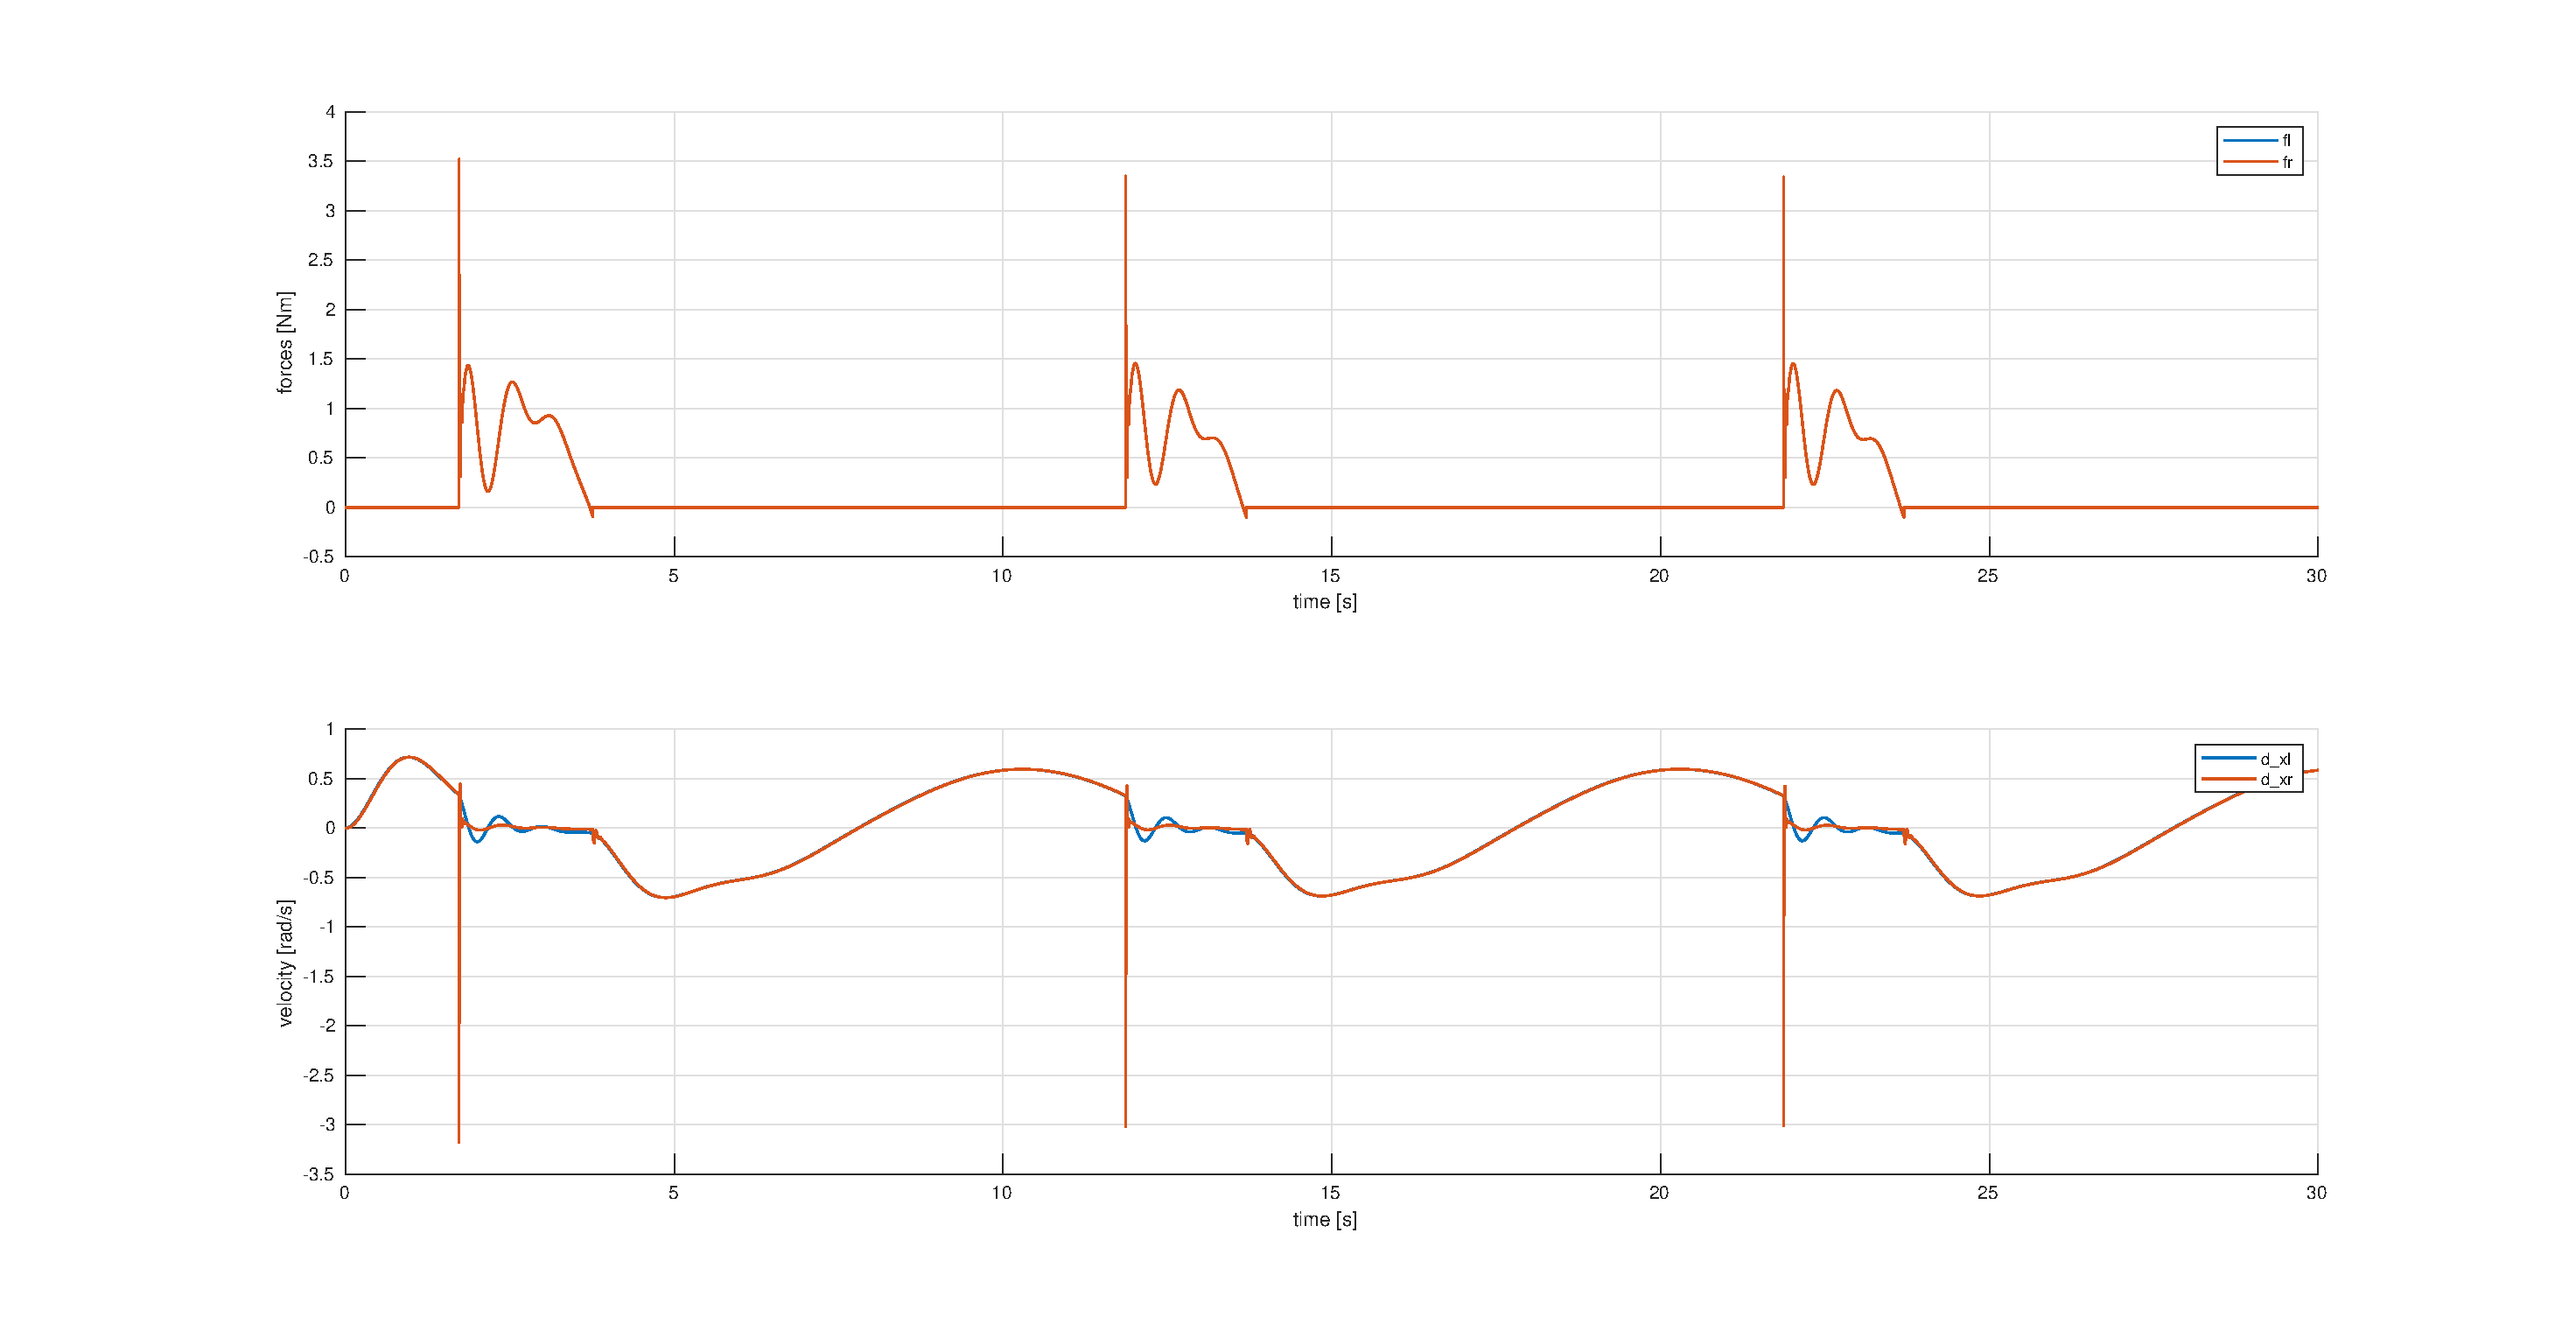
\includegraphics[scale=0.5]{images/scatt_pf.eps}
    \end{center}
    \caption{Scattering based FP variables: they should be identical thanks to the scattering formulation. As it is visible there are some numerical errors corrected partially using a low pass filter in the communication channel}
    \label{fig:scat_var}
\end{figure}

Finally, In Fig \ref{fig:scatt_pf_step} the scattering based architecture FP was evaluated with a step reference in contact. This gives a minimal idea of the interaction forces and the actual position reached by the master and the slave.

\begin{figure}[H]
    \begin{center}
        \hspace*{-4.5cm}
        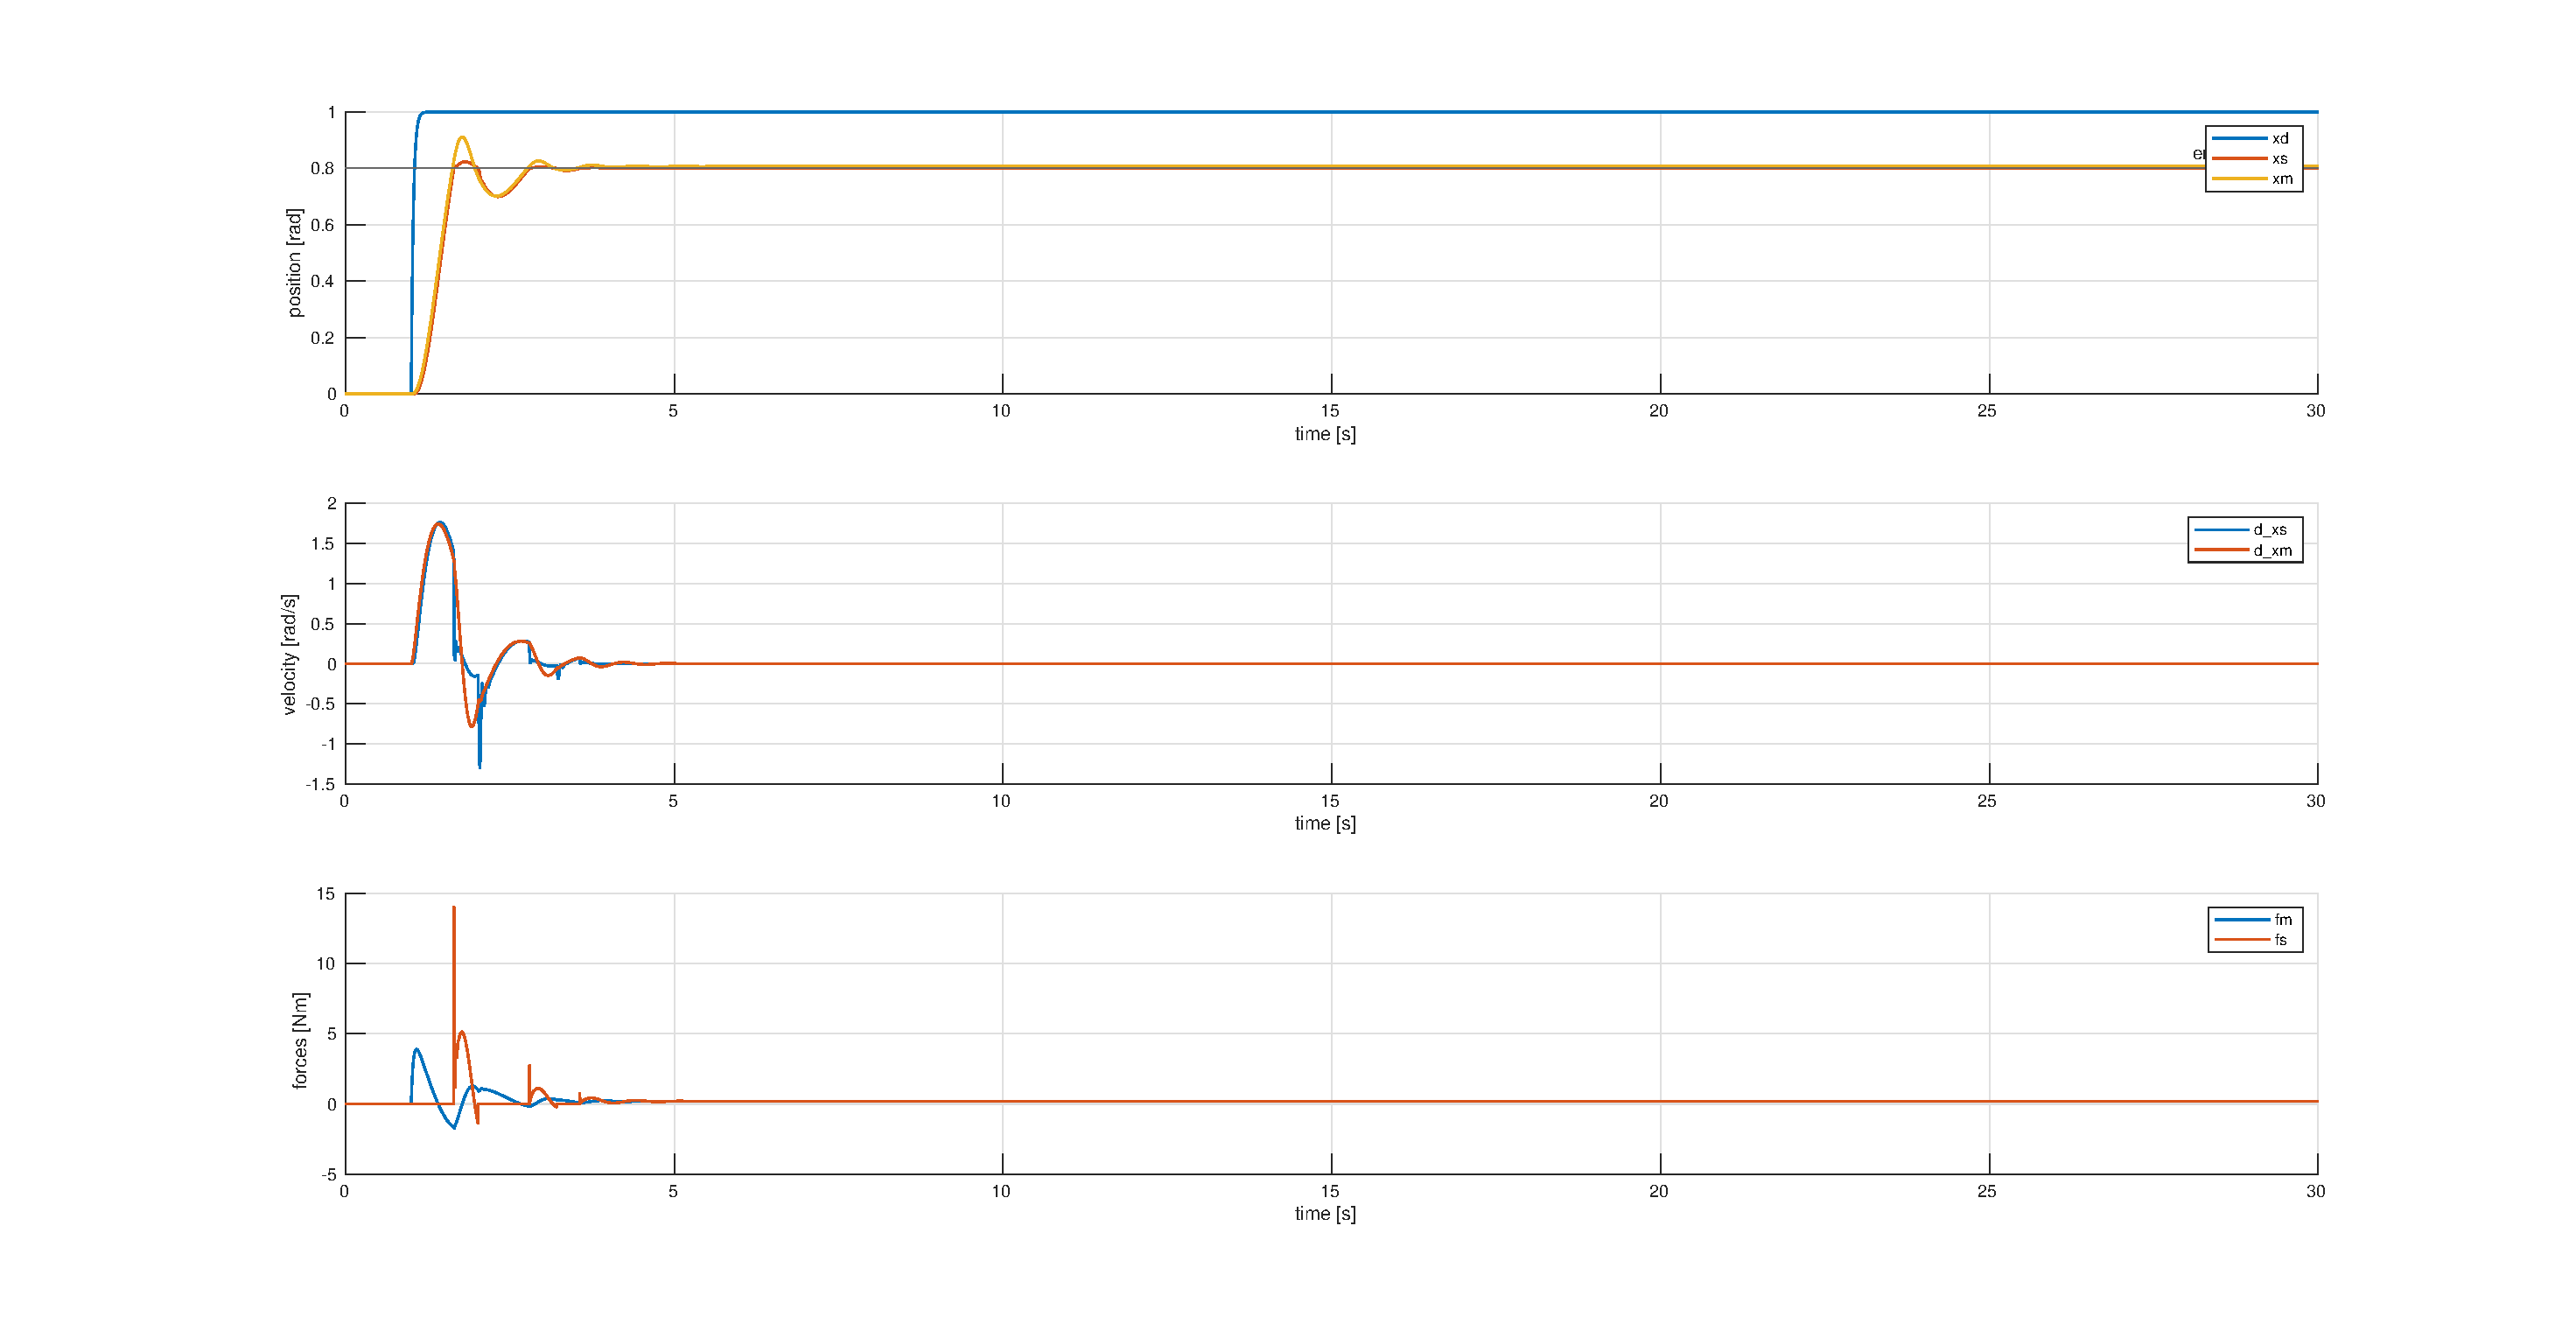
\includegraphics[scale=0.5]{images/scatt_pf_step.eps}
    \end{center}
    \caption{Scattering based FP in contact at 0.8 with step reference. In order to produce this response the integral action from the human intention controller was removed.}
    \label{fig:scatt_pf_step}
\end{figure}

\newpage

\subsection{Scattering based Position-Position}

The idea of the scattering based PP is to use the master and slave force measurements and use the scattering transformations to obtain the velocities on both sides. In this way we have a velocity controller on both slave and master. In this scenario the scattering based architecture Position-Position was evaluated with a delay of 10 time steps in the communication channel. The environment used is $B_e = 10$ and $K_e = 200$. 

\[
    \begin{cases}
    u_l=\sqrt{\frac{2}{b}}F_l-v_l\\
    \dot{x}_l = \frac{1}{b}(F_l-\sqrt{2b}v_l)
    \end{cases}
    \begin{cases}
    u_r=\sqrt{\frac{2}{b}}F_r-v_r\\
    \dot{x}_r=-\frac{1}{b}(F_r-\sqrt{2b}v_r)
    \end{cases}
\]

\bigskip
In Fig \ref{fig:scat_pp_free} the free motion case is reported. As it is visible the system is stable and there is a minimal delay in the position compared to reference $x_d$.

\begin{figure}[H]
    \begin{center}
        \hspace*{-4.5cm}
        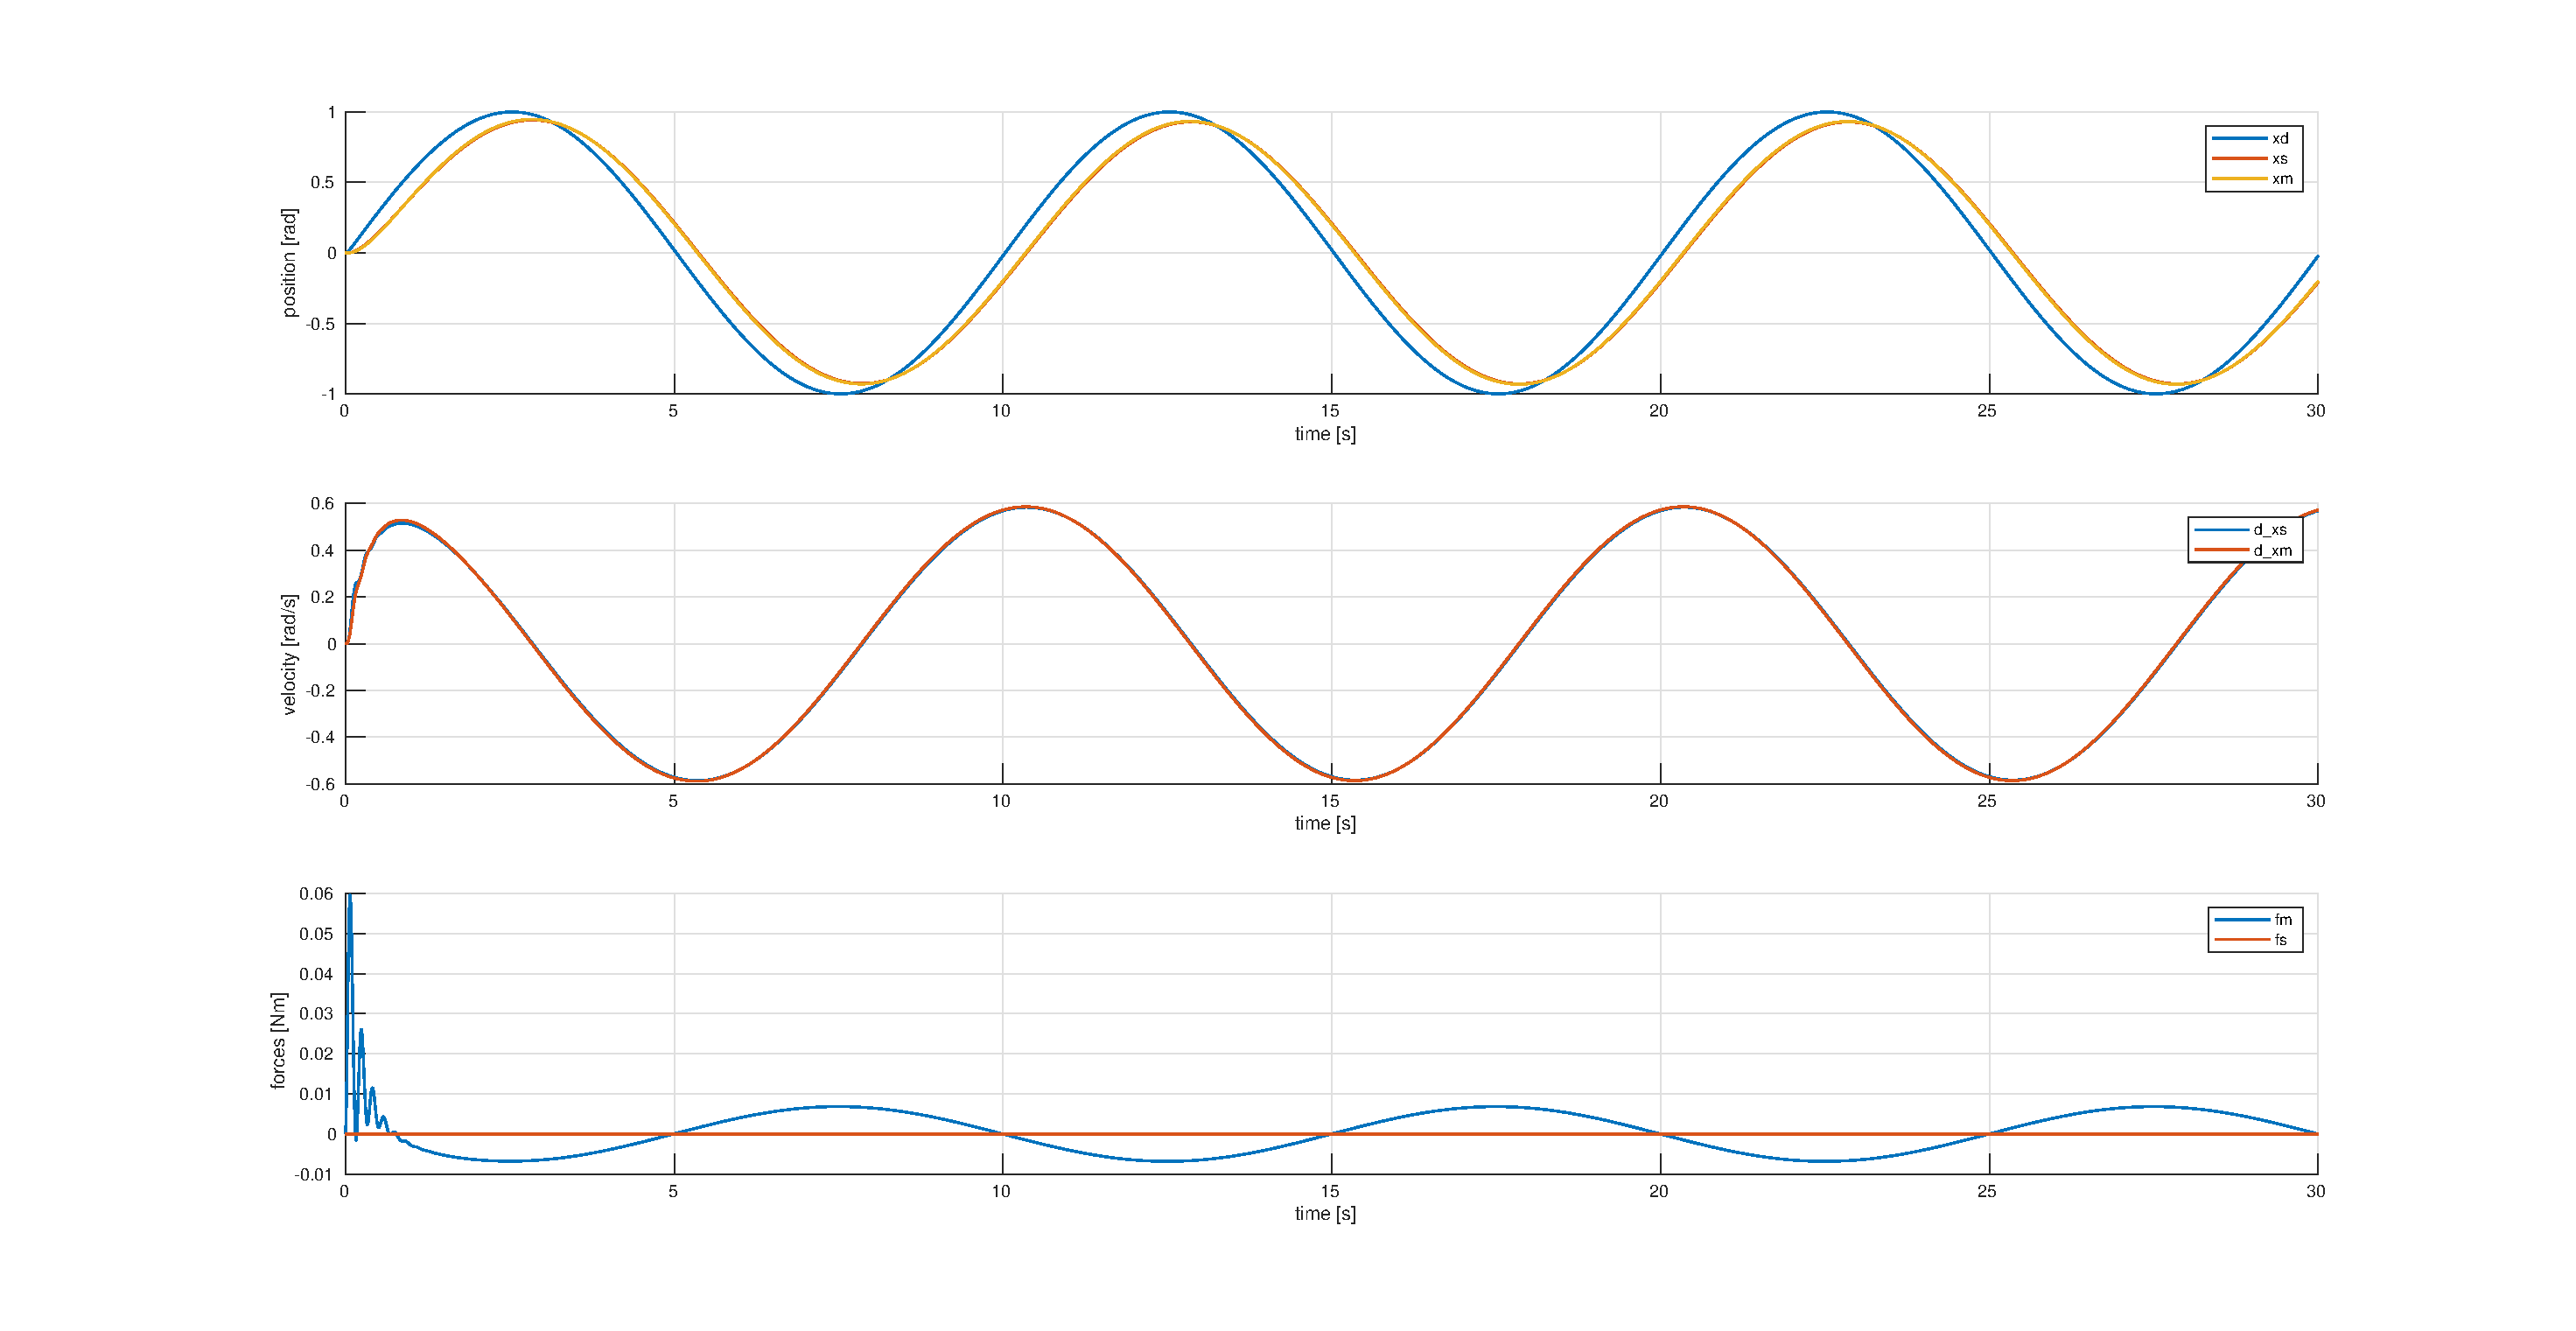
\includegraphics[scale=0.5]{images/scat_pp_free.eps}
    \end{center}
    \caption{Scattering based PP in free motion a low pass filter is introduced in the scattering formulation to correct numerical errors}
    \label{fig:scat_pp_free}
\end{figure}

\newpage
In Fig \ref{fig:scat_pp_contact} the contact case is reported. As it is visible there is some "noise" in the velocities and forces plots: the low pass filter implemented in the communication channel can leverage this problem by decreasing the cut-off frequency. A cut-off frequency of 10 Hz was used to produce the figure.

\begin{figure}[H]
    \begin{center}
        \hspace*{-4.5cm}
        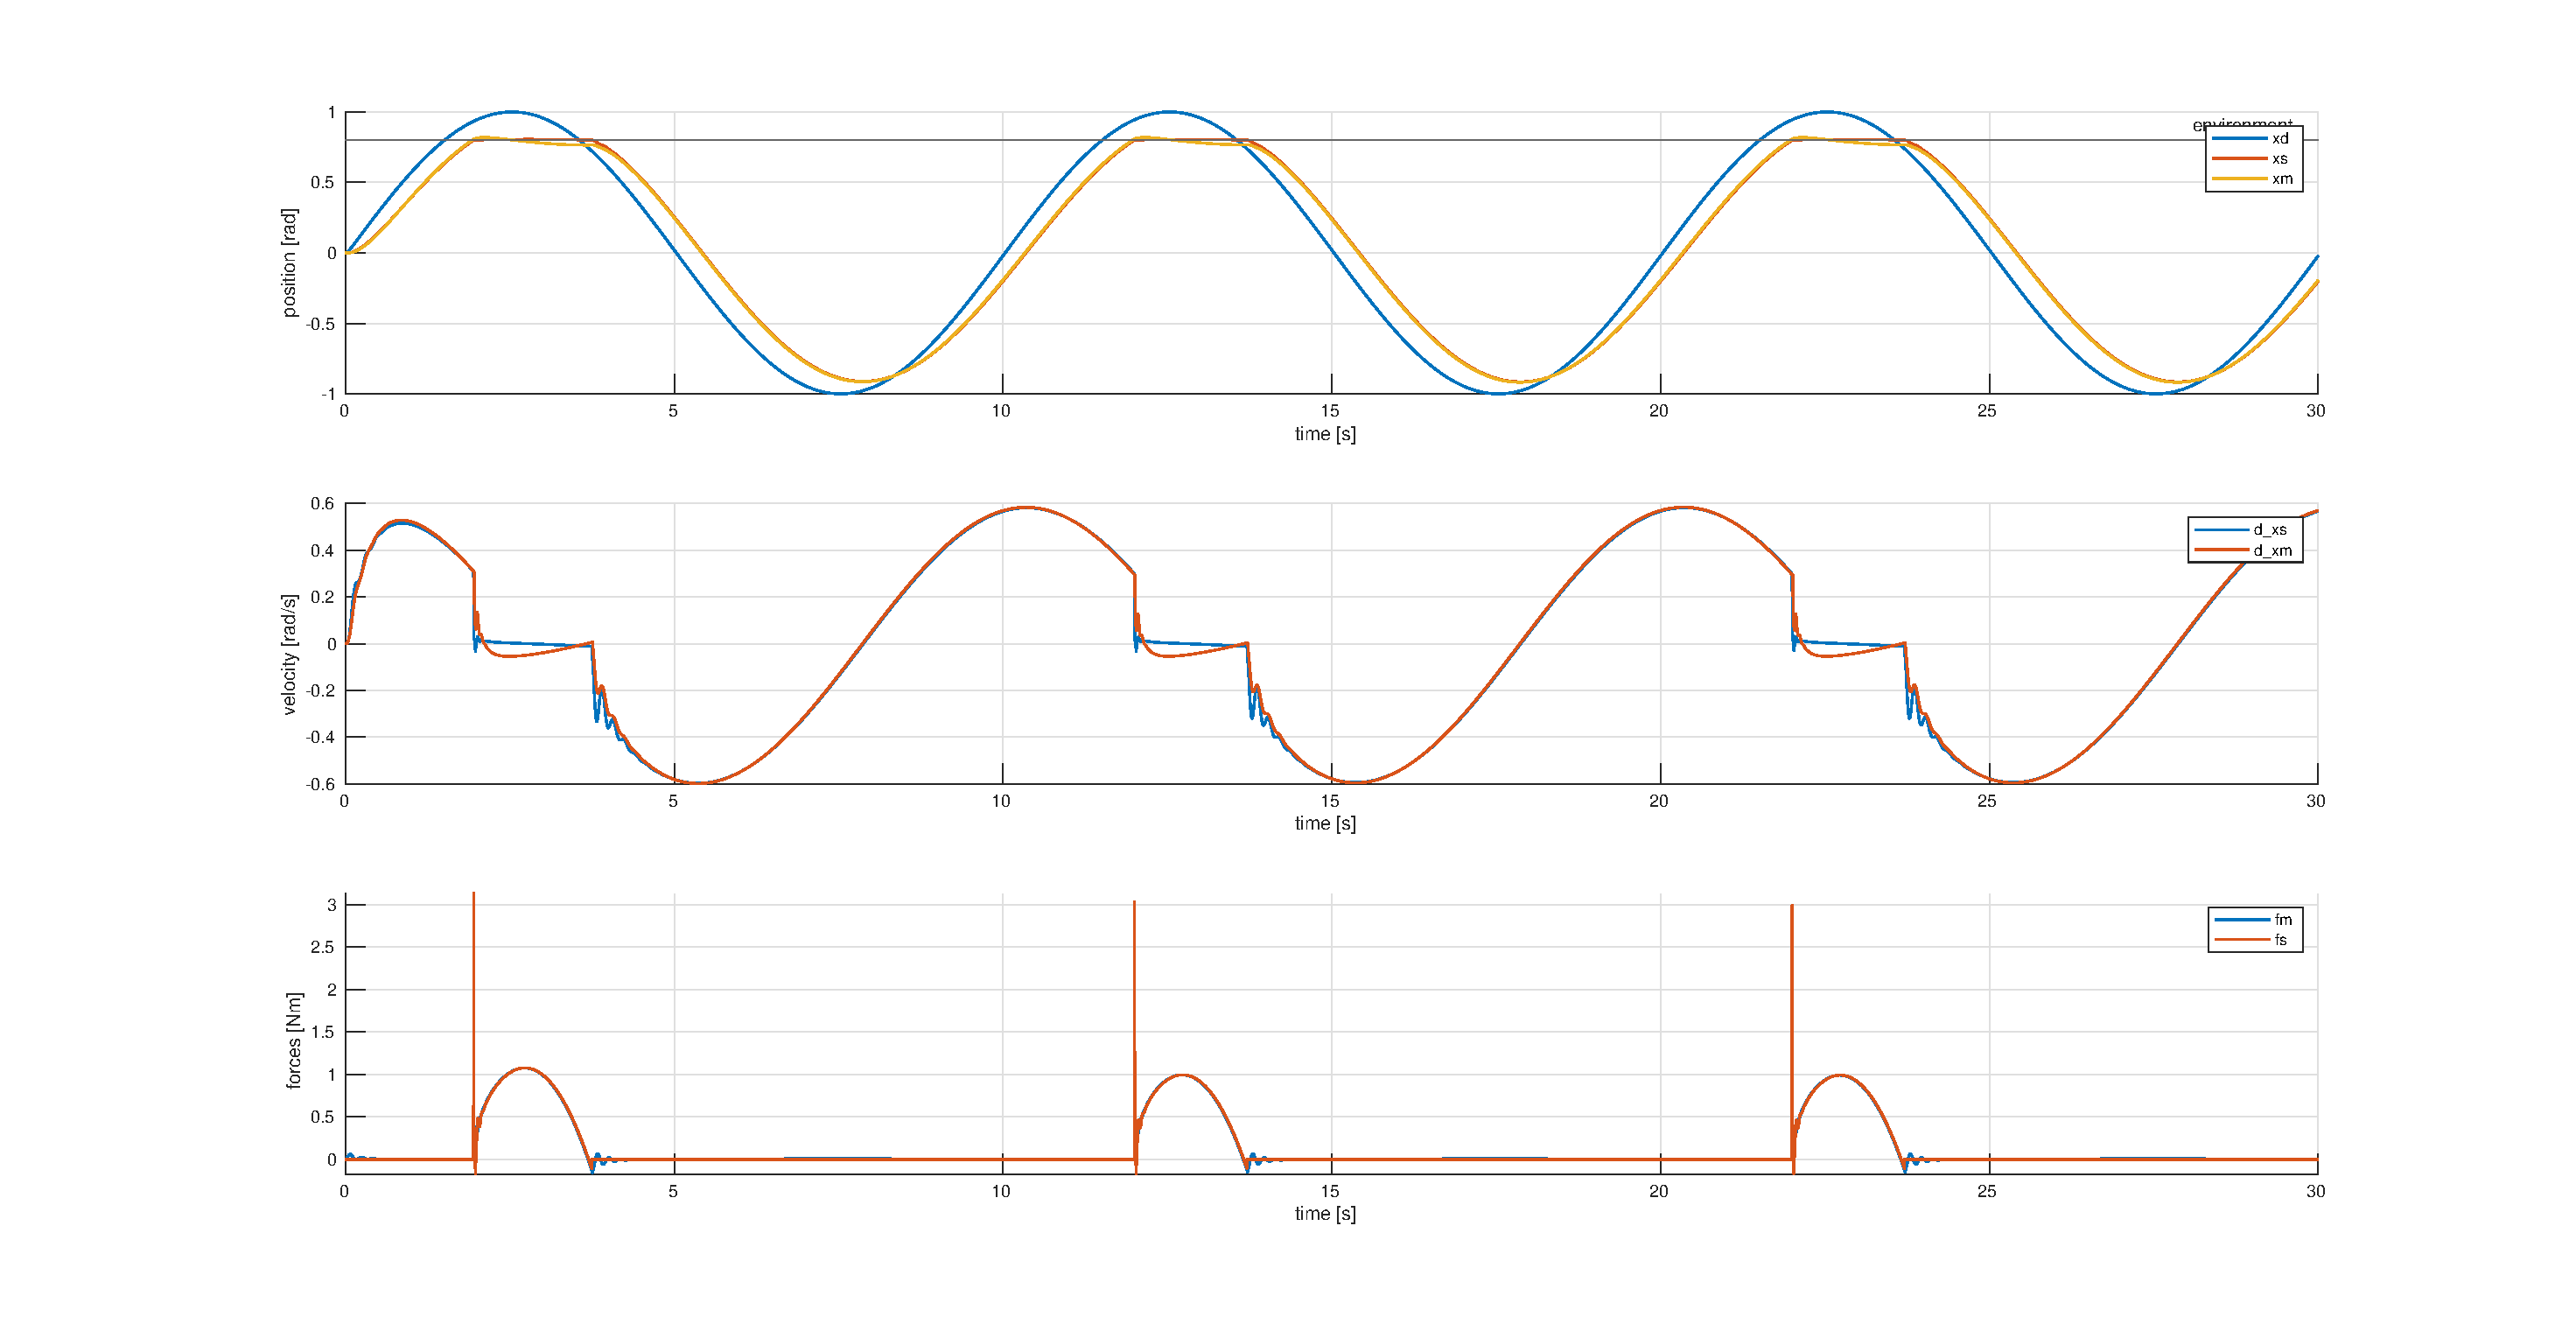
\includegraphics[scale=0.5]{images/scat_pp_contact.eps}
    \end{center}
    \caption{Scattering based PP in contact with a stiff environment at 0.8}
    \label{fig:scat_pp_contact}
\end{figure}

In Fig \ref{fig:scat_pp_contact_kalman} some noise measurements are added, both on velocities and forces, to the architecture as well as a kalman filter to get position and velocity estimations both at master and slave side. Finally the internal low pass filter in the communication channel was introduced with a cut-off frequency of 10Hz. As it is visible both the velocities and the forces are affected by noise.

\begin{figure}[H]
    \begin{center}
        \hspace*{-4.5cm}
        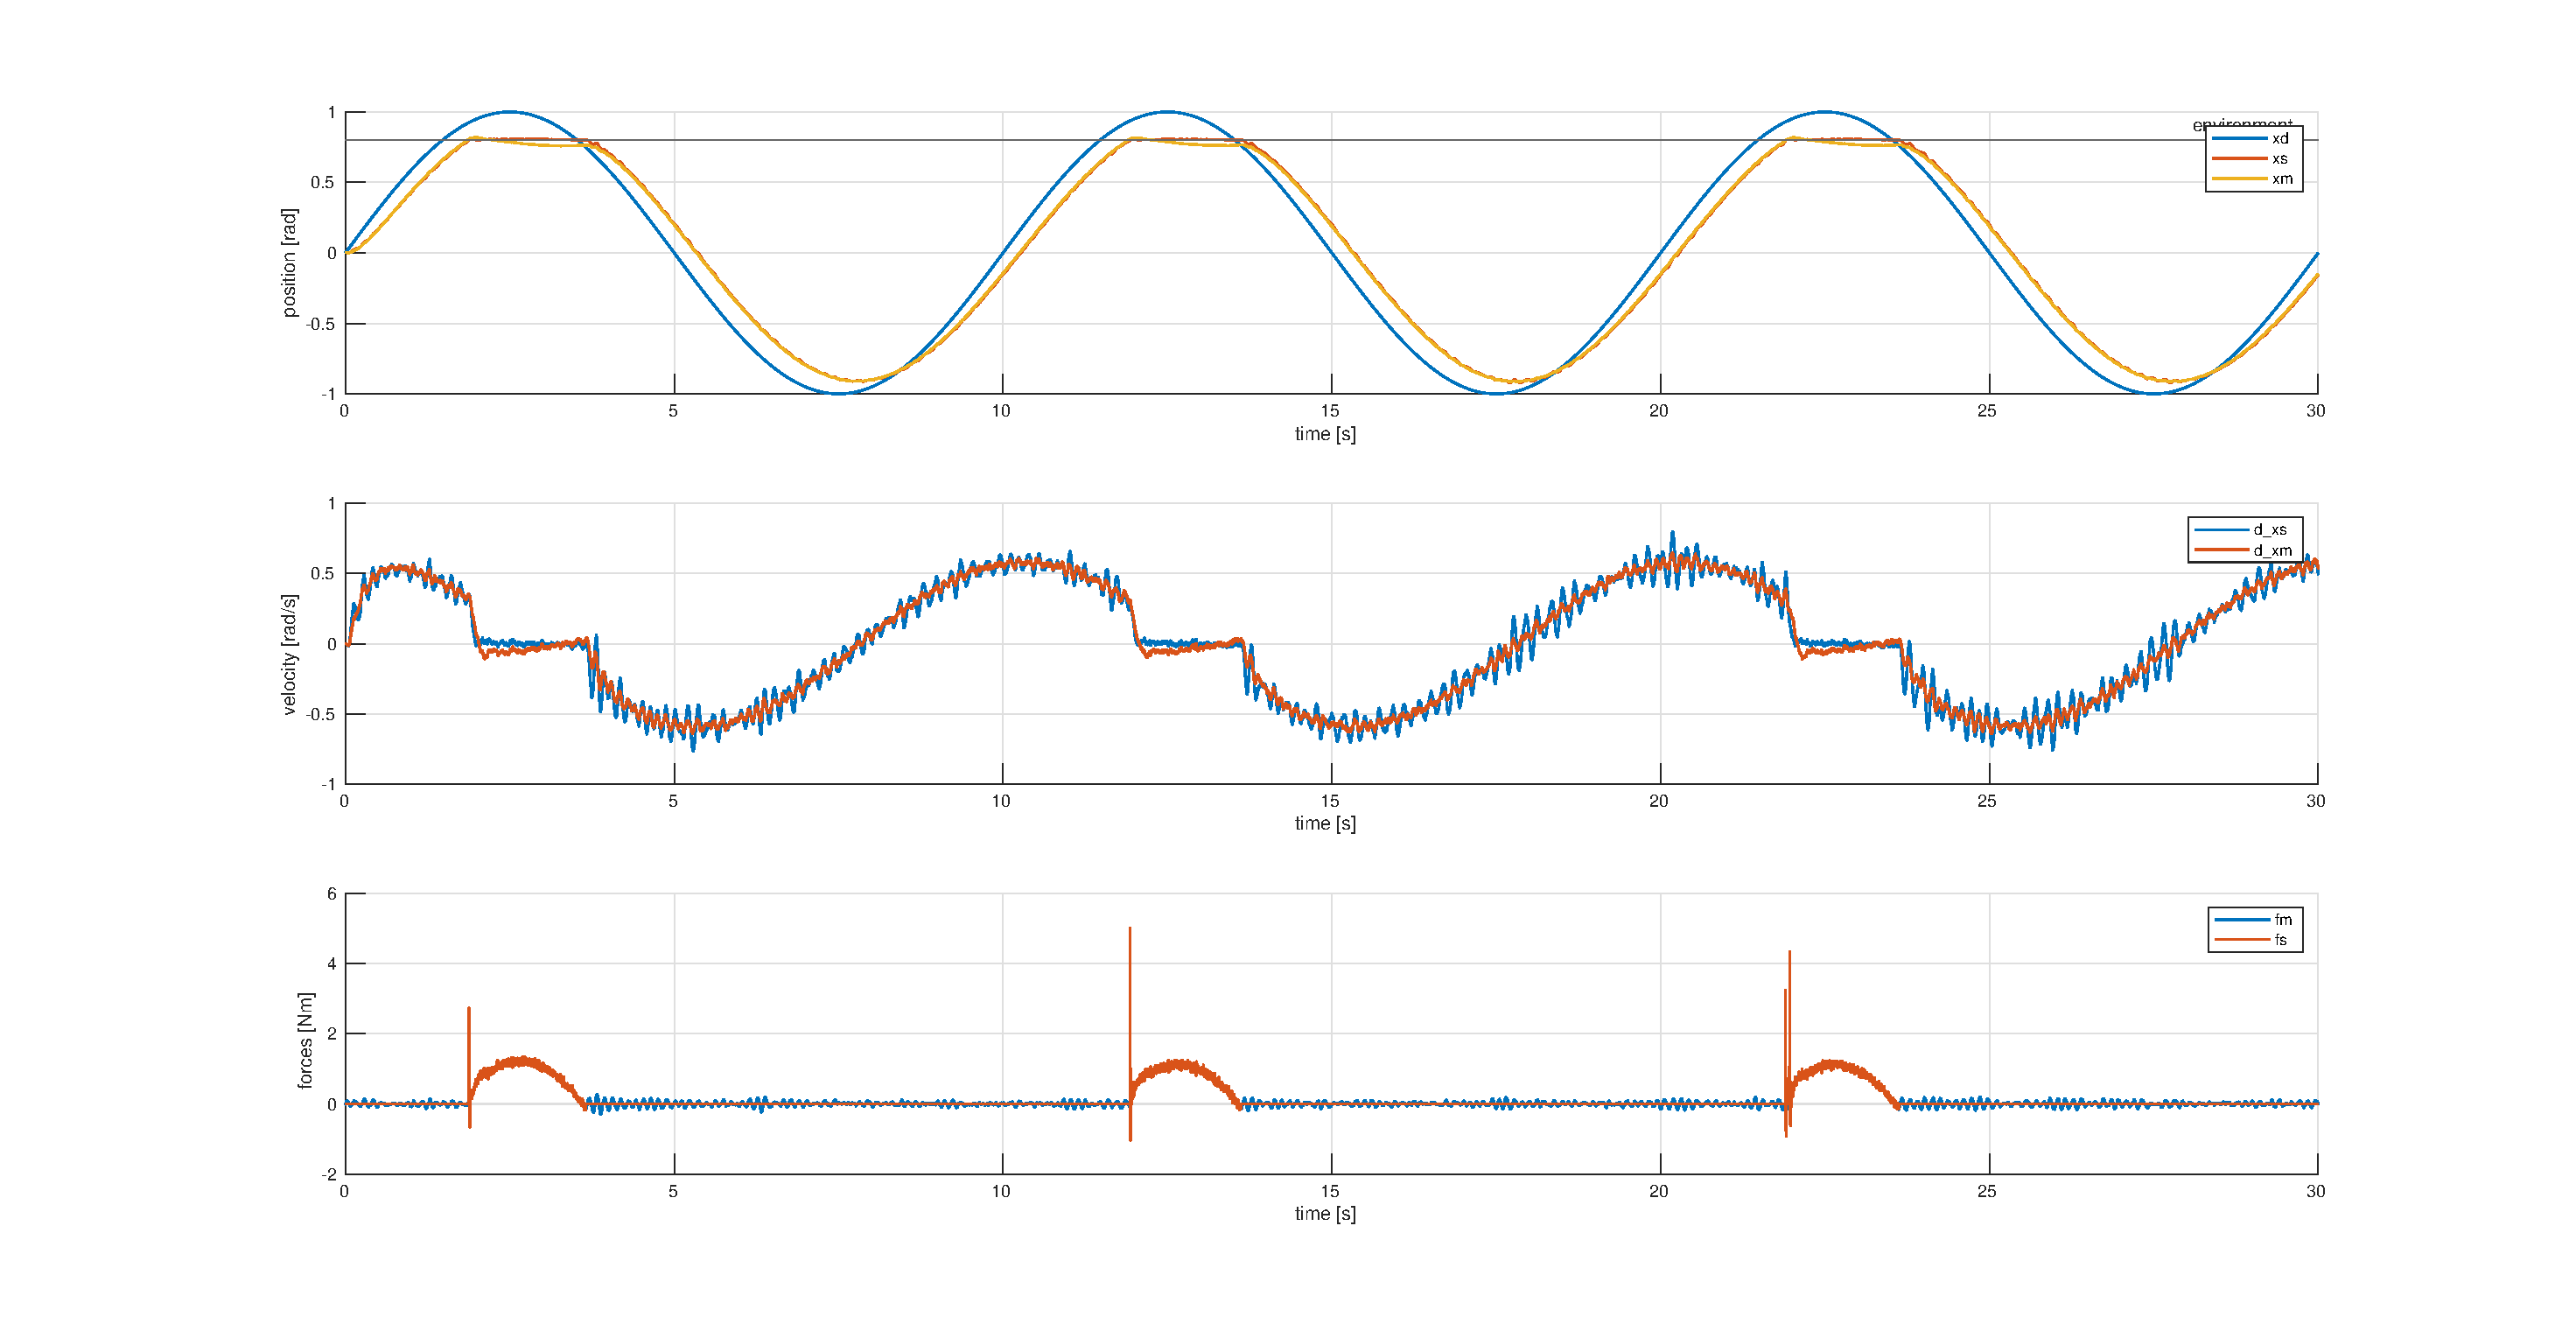
\includegraphics[scale=0.5]{images/scat_pp_contact_kalman.eps}
    \end{center}
    \caption{Scattering based PP with noisy measurements and kalman filters in contact with a stiff environment at 0.8 and delay 2 time steps}
    \label{fig:scat_pp_contact_kalman}
\end{figure}

Finally, In Fig \ref{fig:scatt_pp_step} the scattering based architecture PP was evaluated with a step reference in contact. This gives a minimal idea of the interaction forces and the actual position reached by the master and the slave.

\begin{figure}[H]
    \begin{center}
        \hspace*{-4.5cm}
        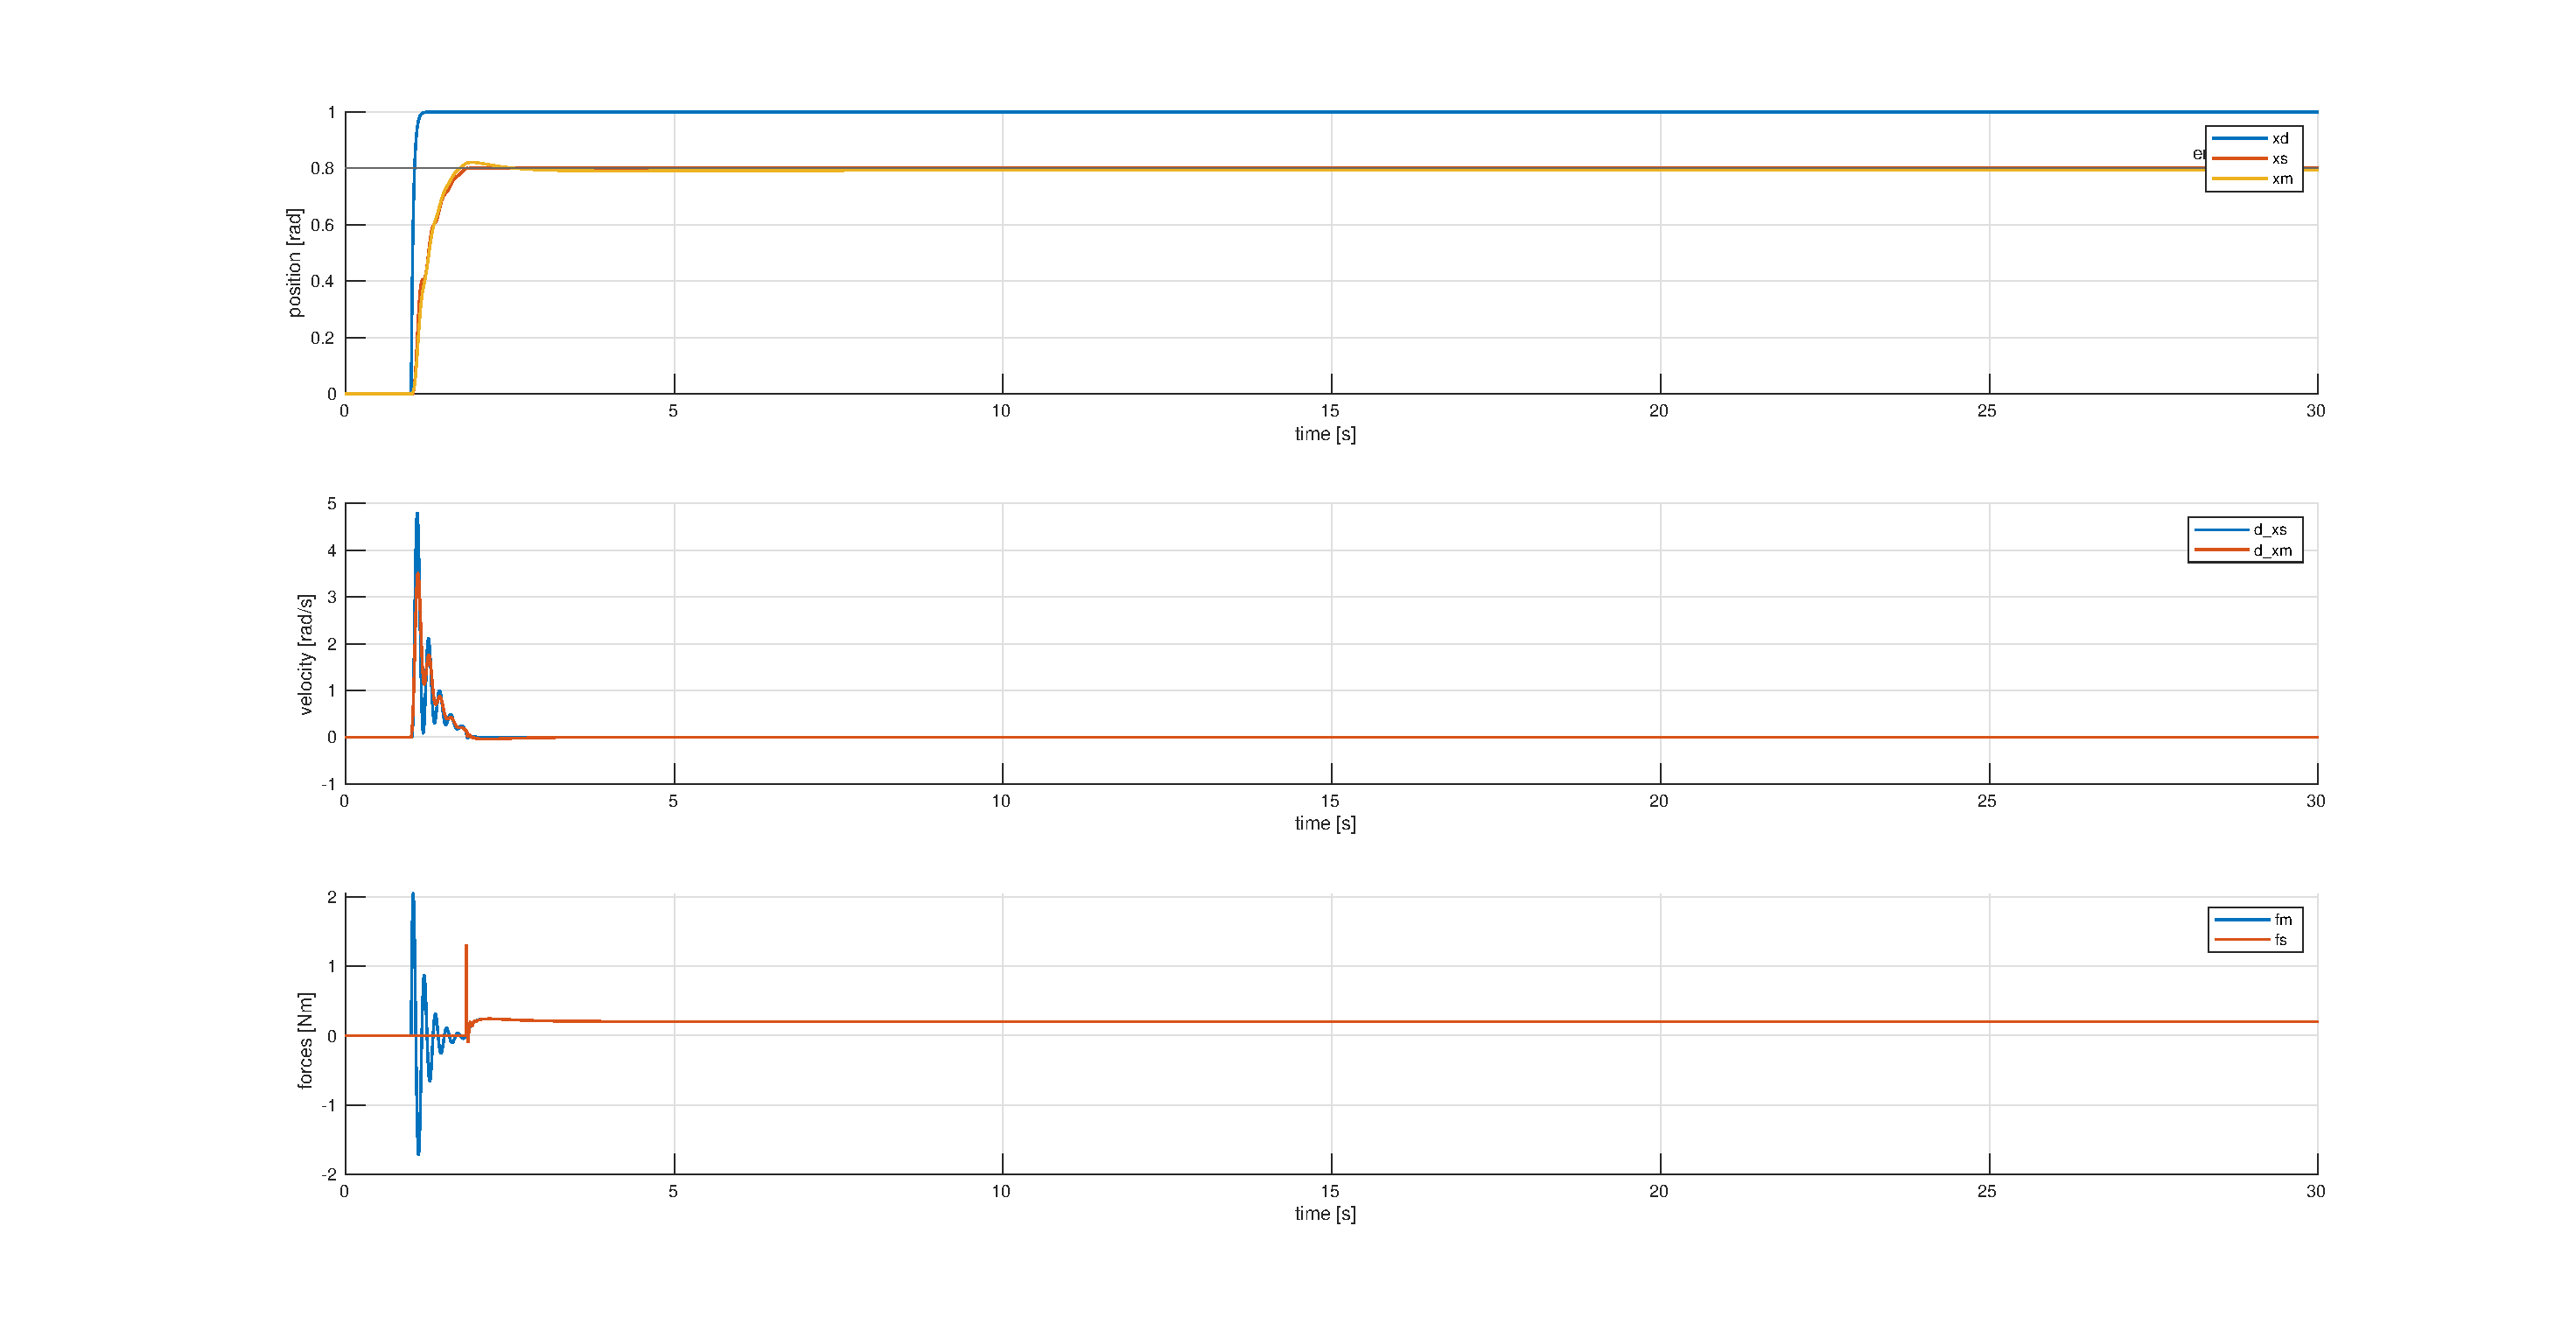
\includegraphics[scale=0.5]{images/scatt_pp_step.eps}
    \end{center}
    \caption{Scattering based PP in contact at 0.8 with step reference. In order to produce this response the integral action from the human intention controller was removed.}
    \label{fig:scatt_pp_step}
\end{figure}

\subsection{Other considerations}

The aim of the architecture is to use passivity to stay stable in presence of delays. In order to verify this assumption a delay of $400$ time steps was used to "break" the original implementation without scattering variables and compared against the use of scattering variables as it is reported in Fig \ref{fig:delay_comp}. In general it is not easy to find such a case even in simulated models and it required a lot of trials.

\begin{figure}[H]
    \hspace*{-3.5cm}
    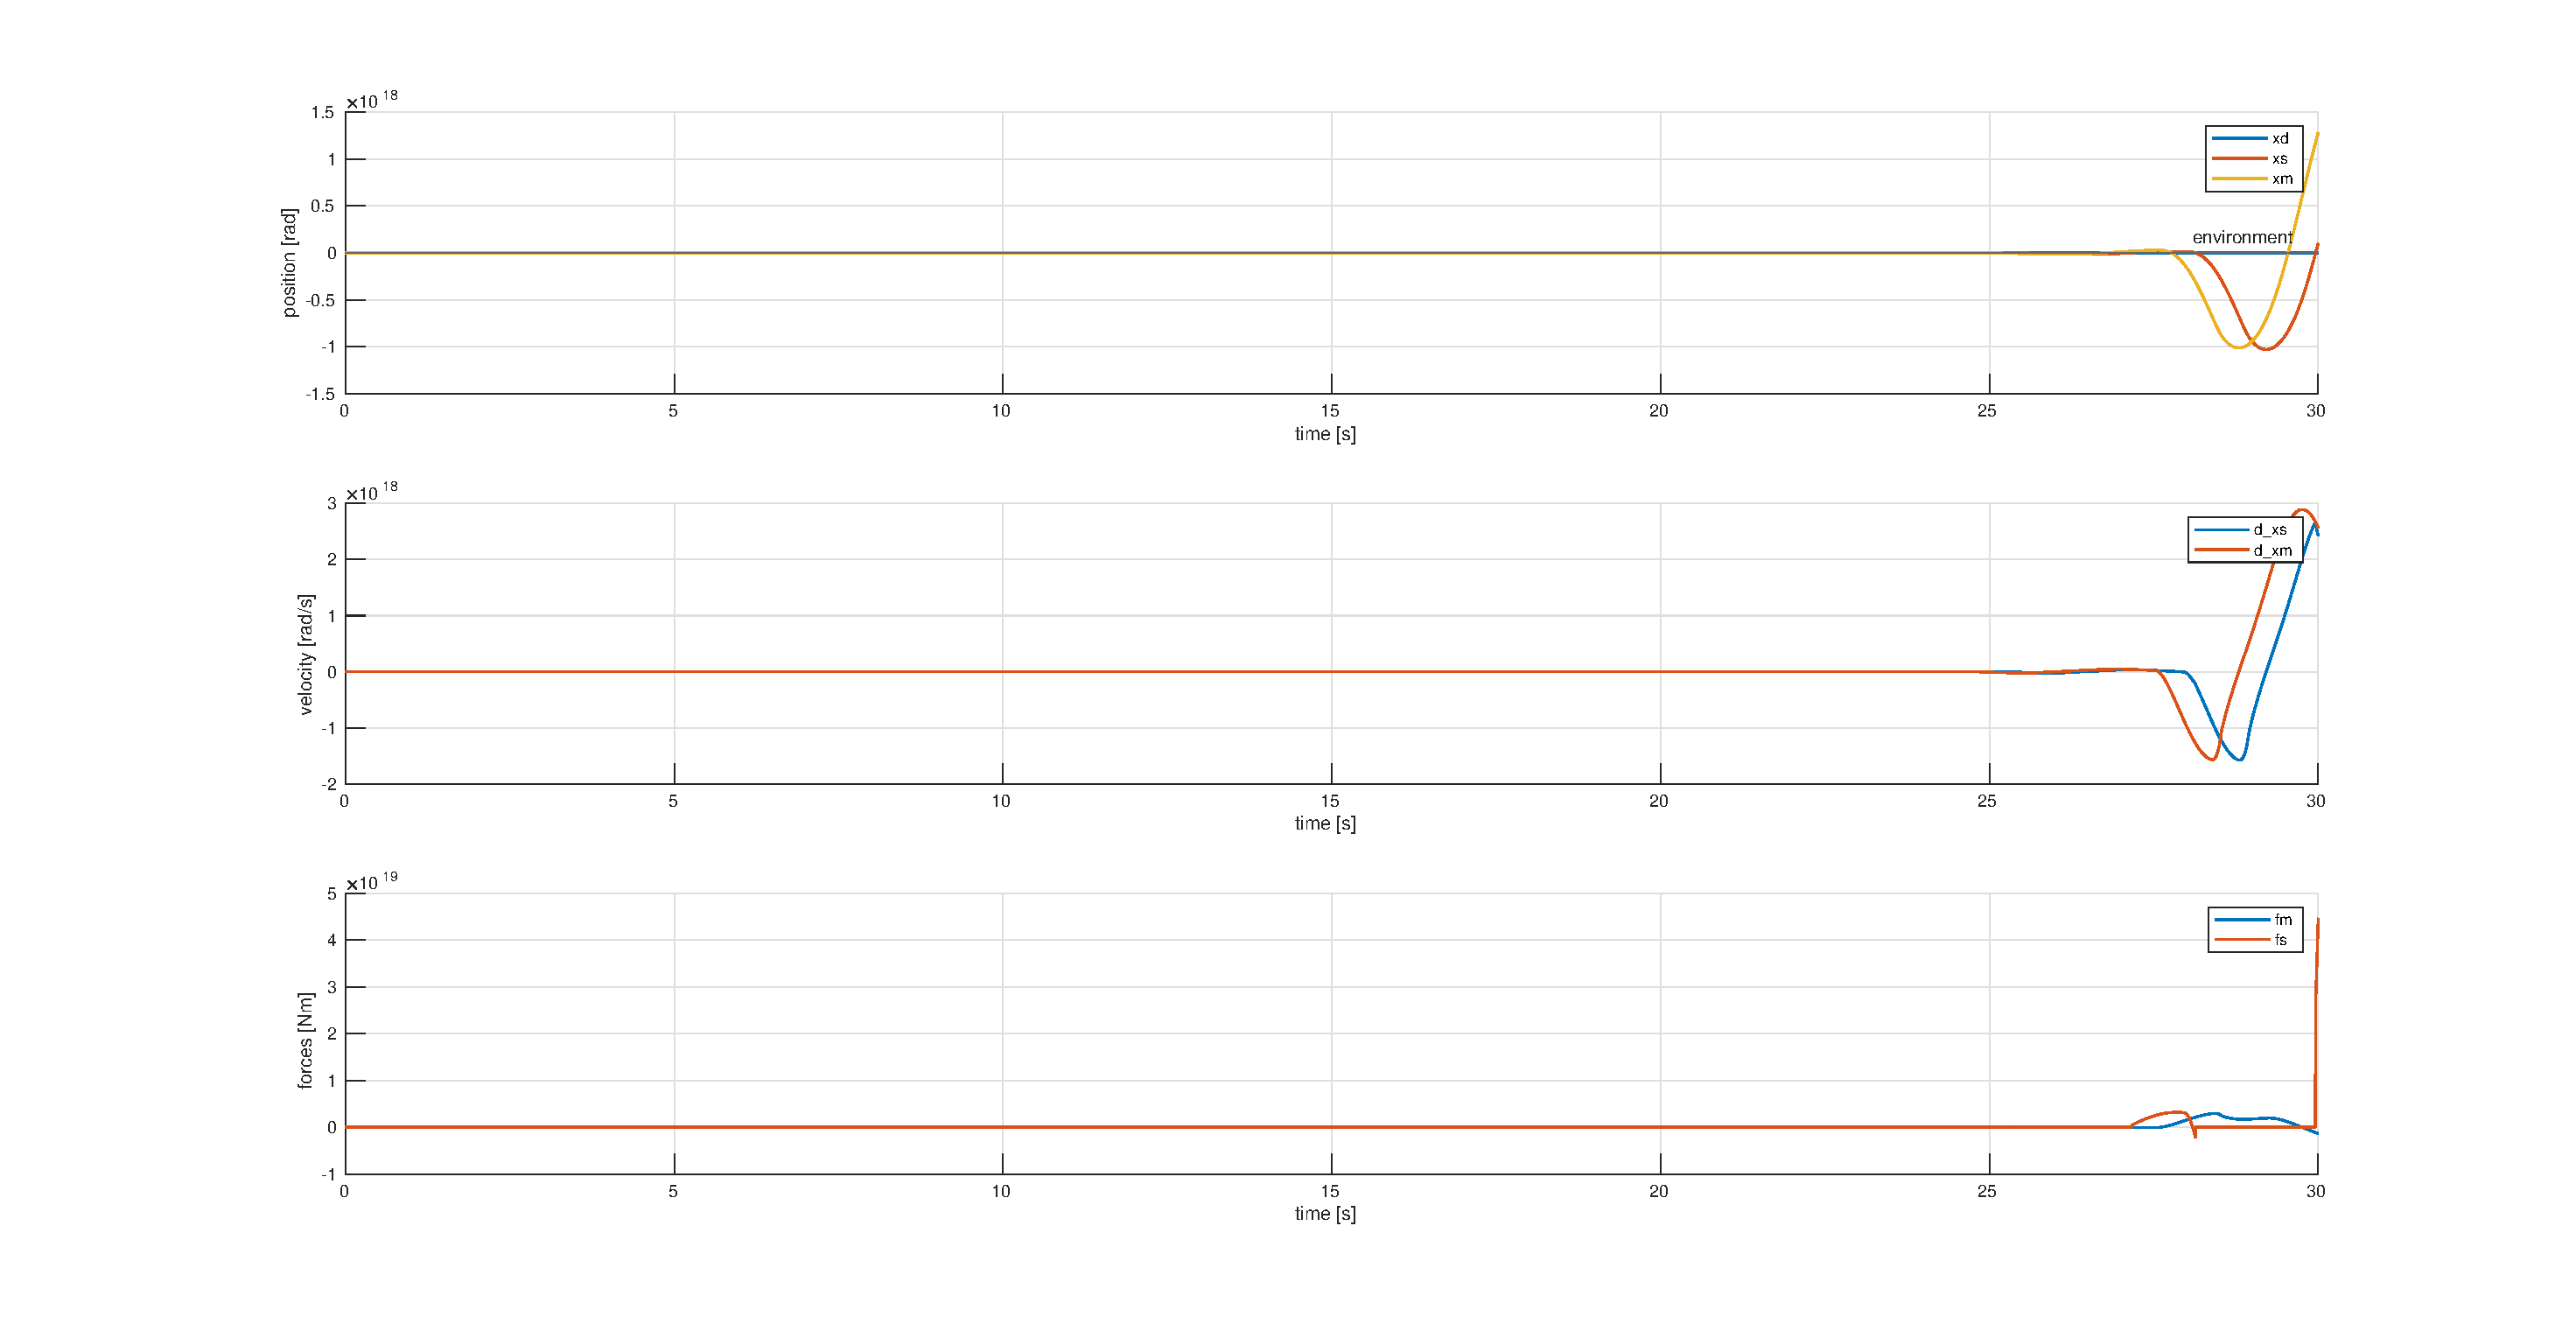
\includegraphics[scale=0.45]{images/scatt_high_delay.eps}
    \qquad
    \hspace*{-3.5cm}
    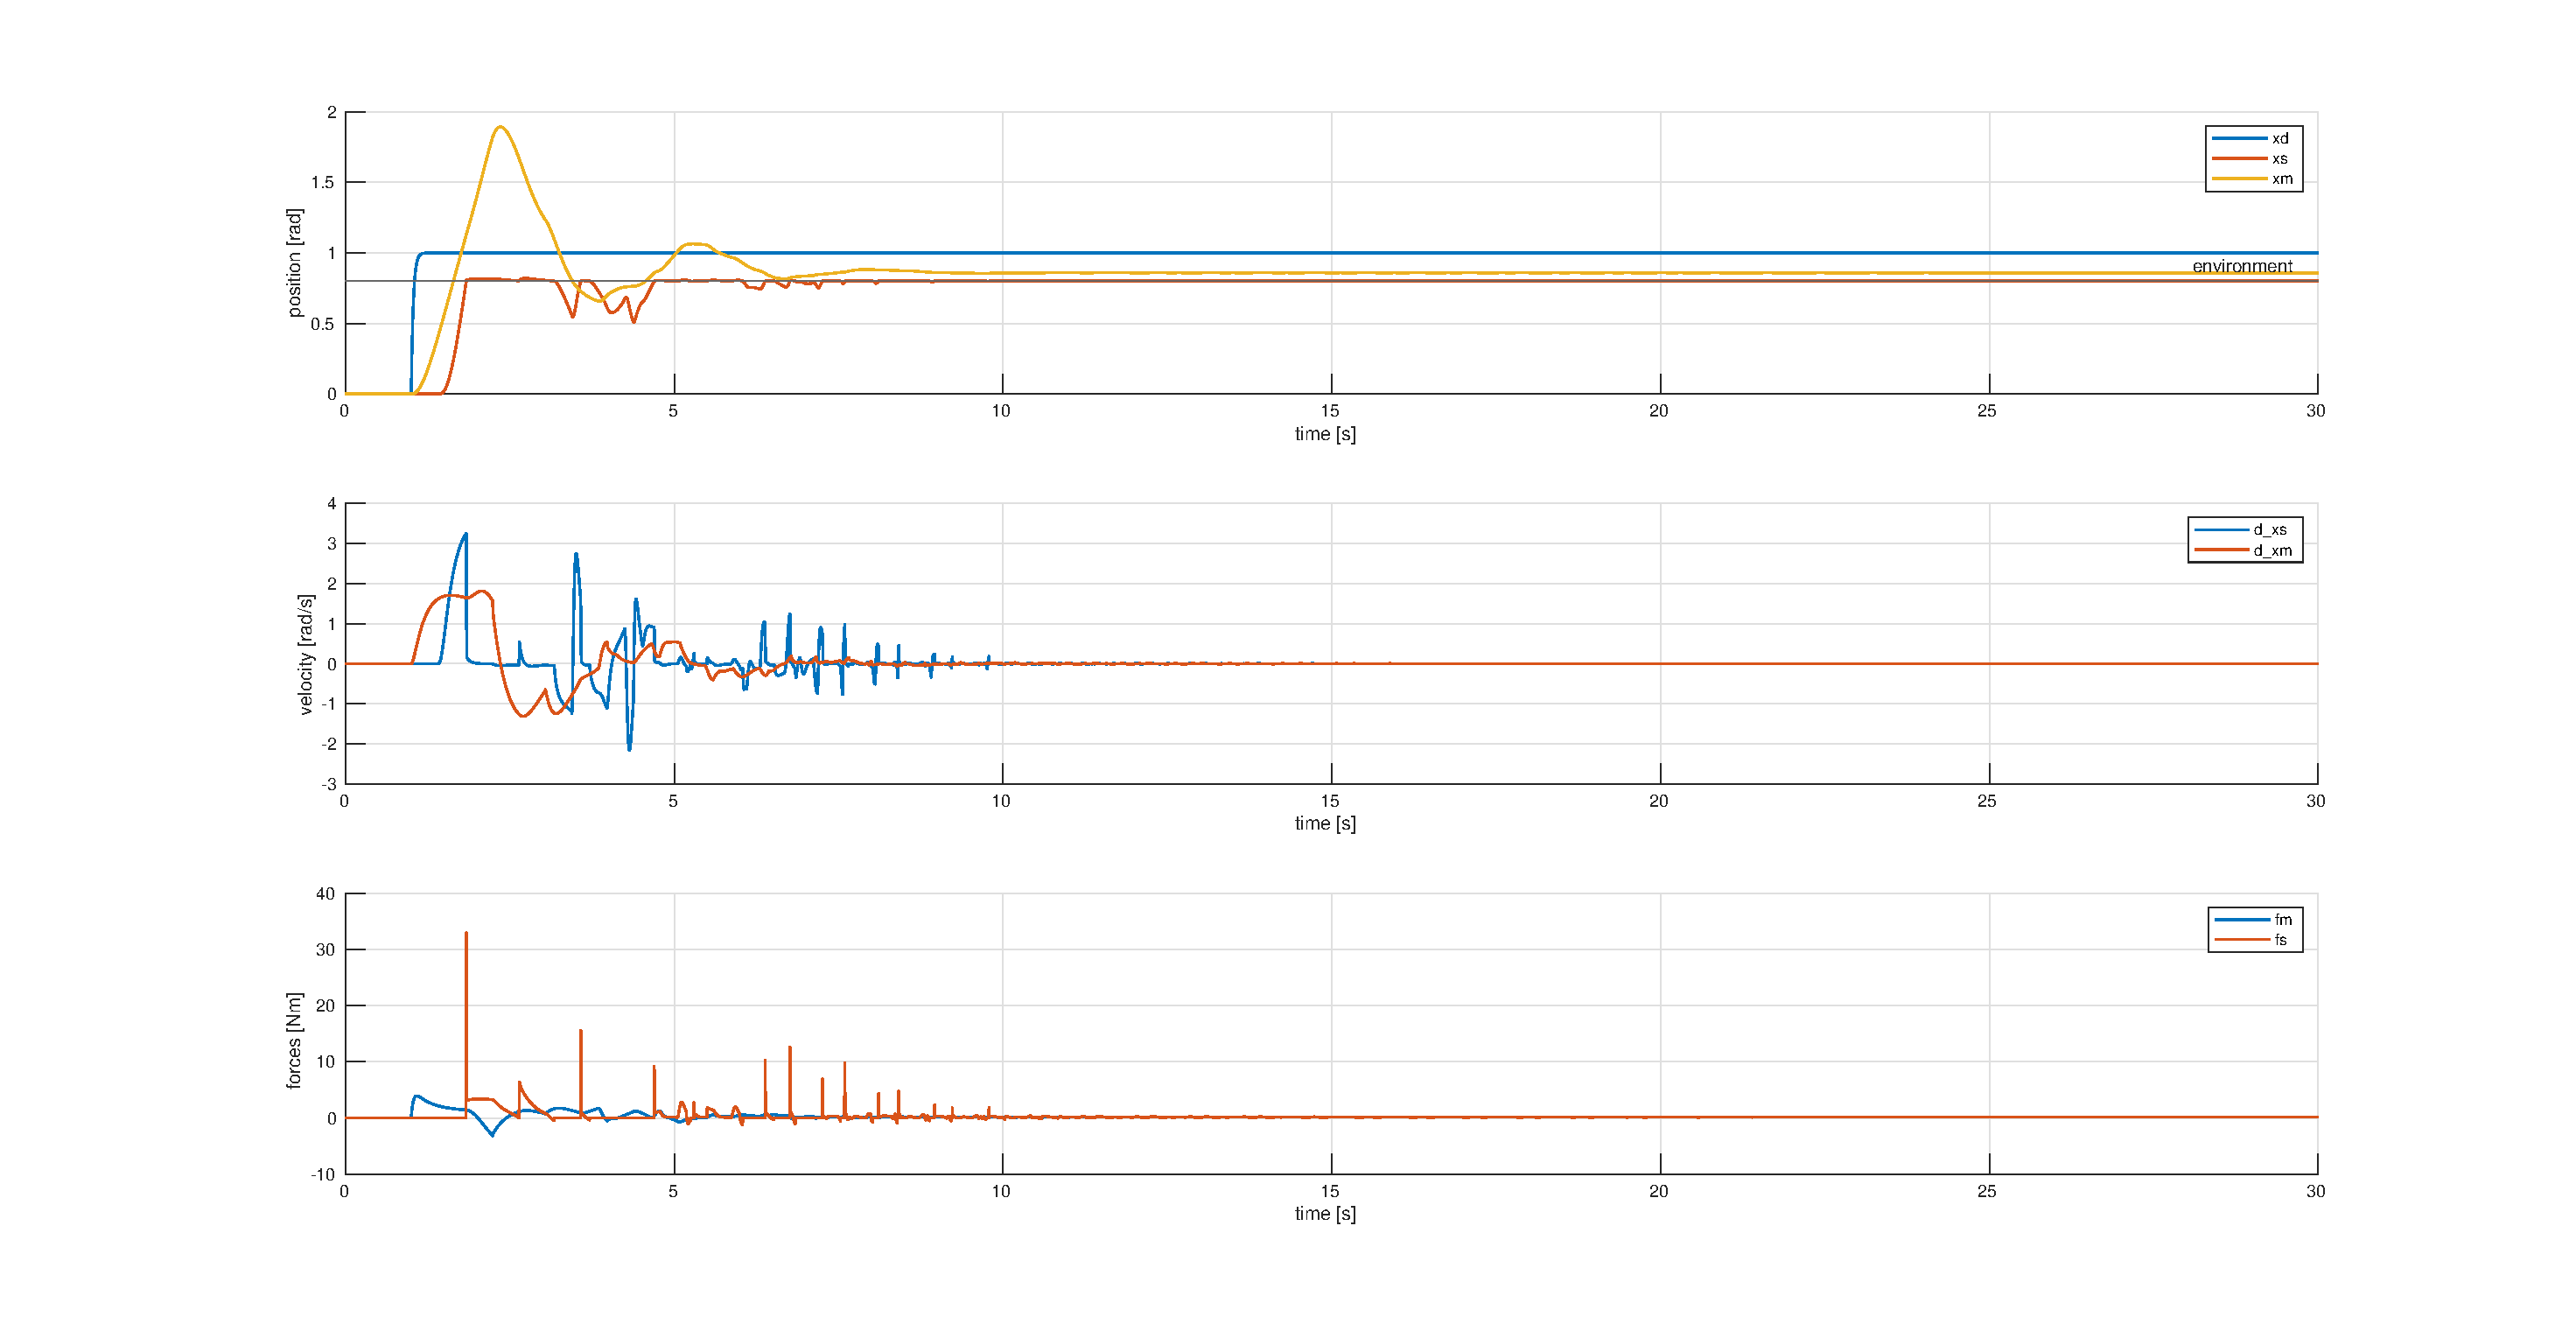
\includegraphics[scale=0.45]{images/scatt_high_delay_comp.eps}
    \caption{First on top: FP architecture without scattering formulation with 400 delay time steps. Second from top: Scattering FP architecture with 400 delay time steps}
    \label{fig:delay_comp}
\end{figure}

\newpage
\section{Two-Layer bilateral teleoperation architecture}

The Two-layer bilateral teleoperation for transparency and passivity was firstly introduced in \textit{Bilateral Telemanipulation With Time Delays:
A Two-Layer Approach Combining Passivity
and Transparency} and the core idea is to
 \begin{quote}
guarantee the stable behavior of bilateral telemanipulation systems in the presence of time-varying destabilizing factors. The approach splits the control architecture into two separate layers. The hierarchical top layer is used
to implement a strategy that addresses the desired transparency,
and the lower layer ensures that no “virtual” energy is generated.
\end{quote}
In Fig \ref{fig:layer} the transparency and passivity layers and their interactions are briefly reported.
\begin{figure}[H]
    \begin{center}
        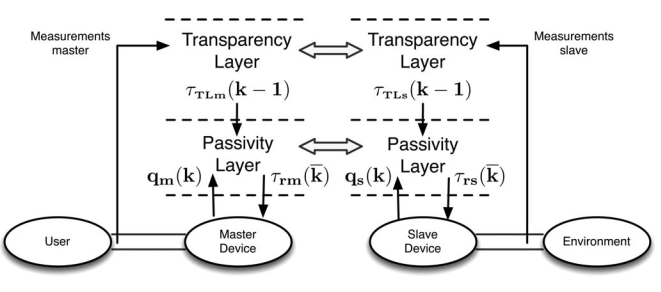
\includegraphics[scale=0.6]{images/layer.png}
    \end{center}
    \caption{Two-layer algorithm for bilateral telemanipulation: Double connections indicate an energetic interaction, taken from \cite{Franken11}}
    \label{fig:layer}
\end{figure}

The core idea in the passivity layer is to maintain an energy tank defined as follow:
\[
    H(k) = H(\overline{k}) + H_{+}(k) - \Delta H_I(k)
\]

where $H(\overline{k})$ is the energy from the past or previous step, $ H_{+}(k)$ is the energy exchanged from the slave side as energy packet and $\Delta H_I(k)$ is the actual energy spent at step $k$ computed as follow:

\[
    \Delta H_I(k) = \tau(\overline{k}) \Delta q(k)
\]
In Fig \ref{fig:architecture} the entire workflow is reported from the original paper describing both master and slave side.
\begin{figure}[H]
    \begin{center}
        \hspace*{-2.2cm}
        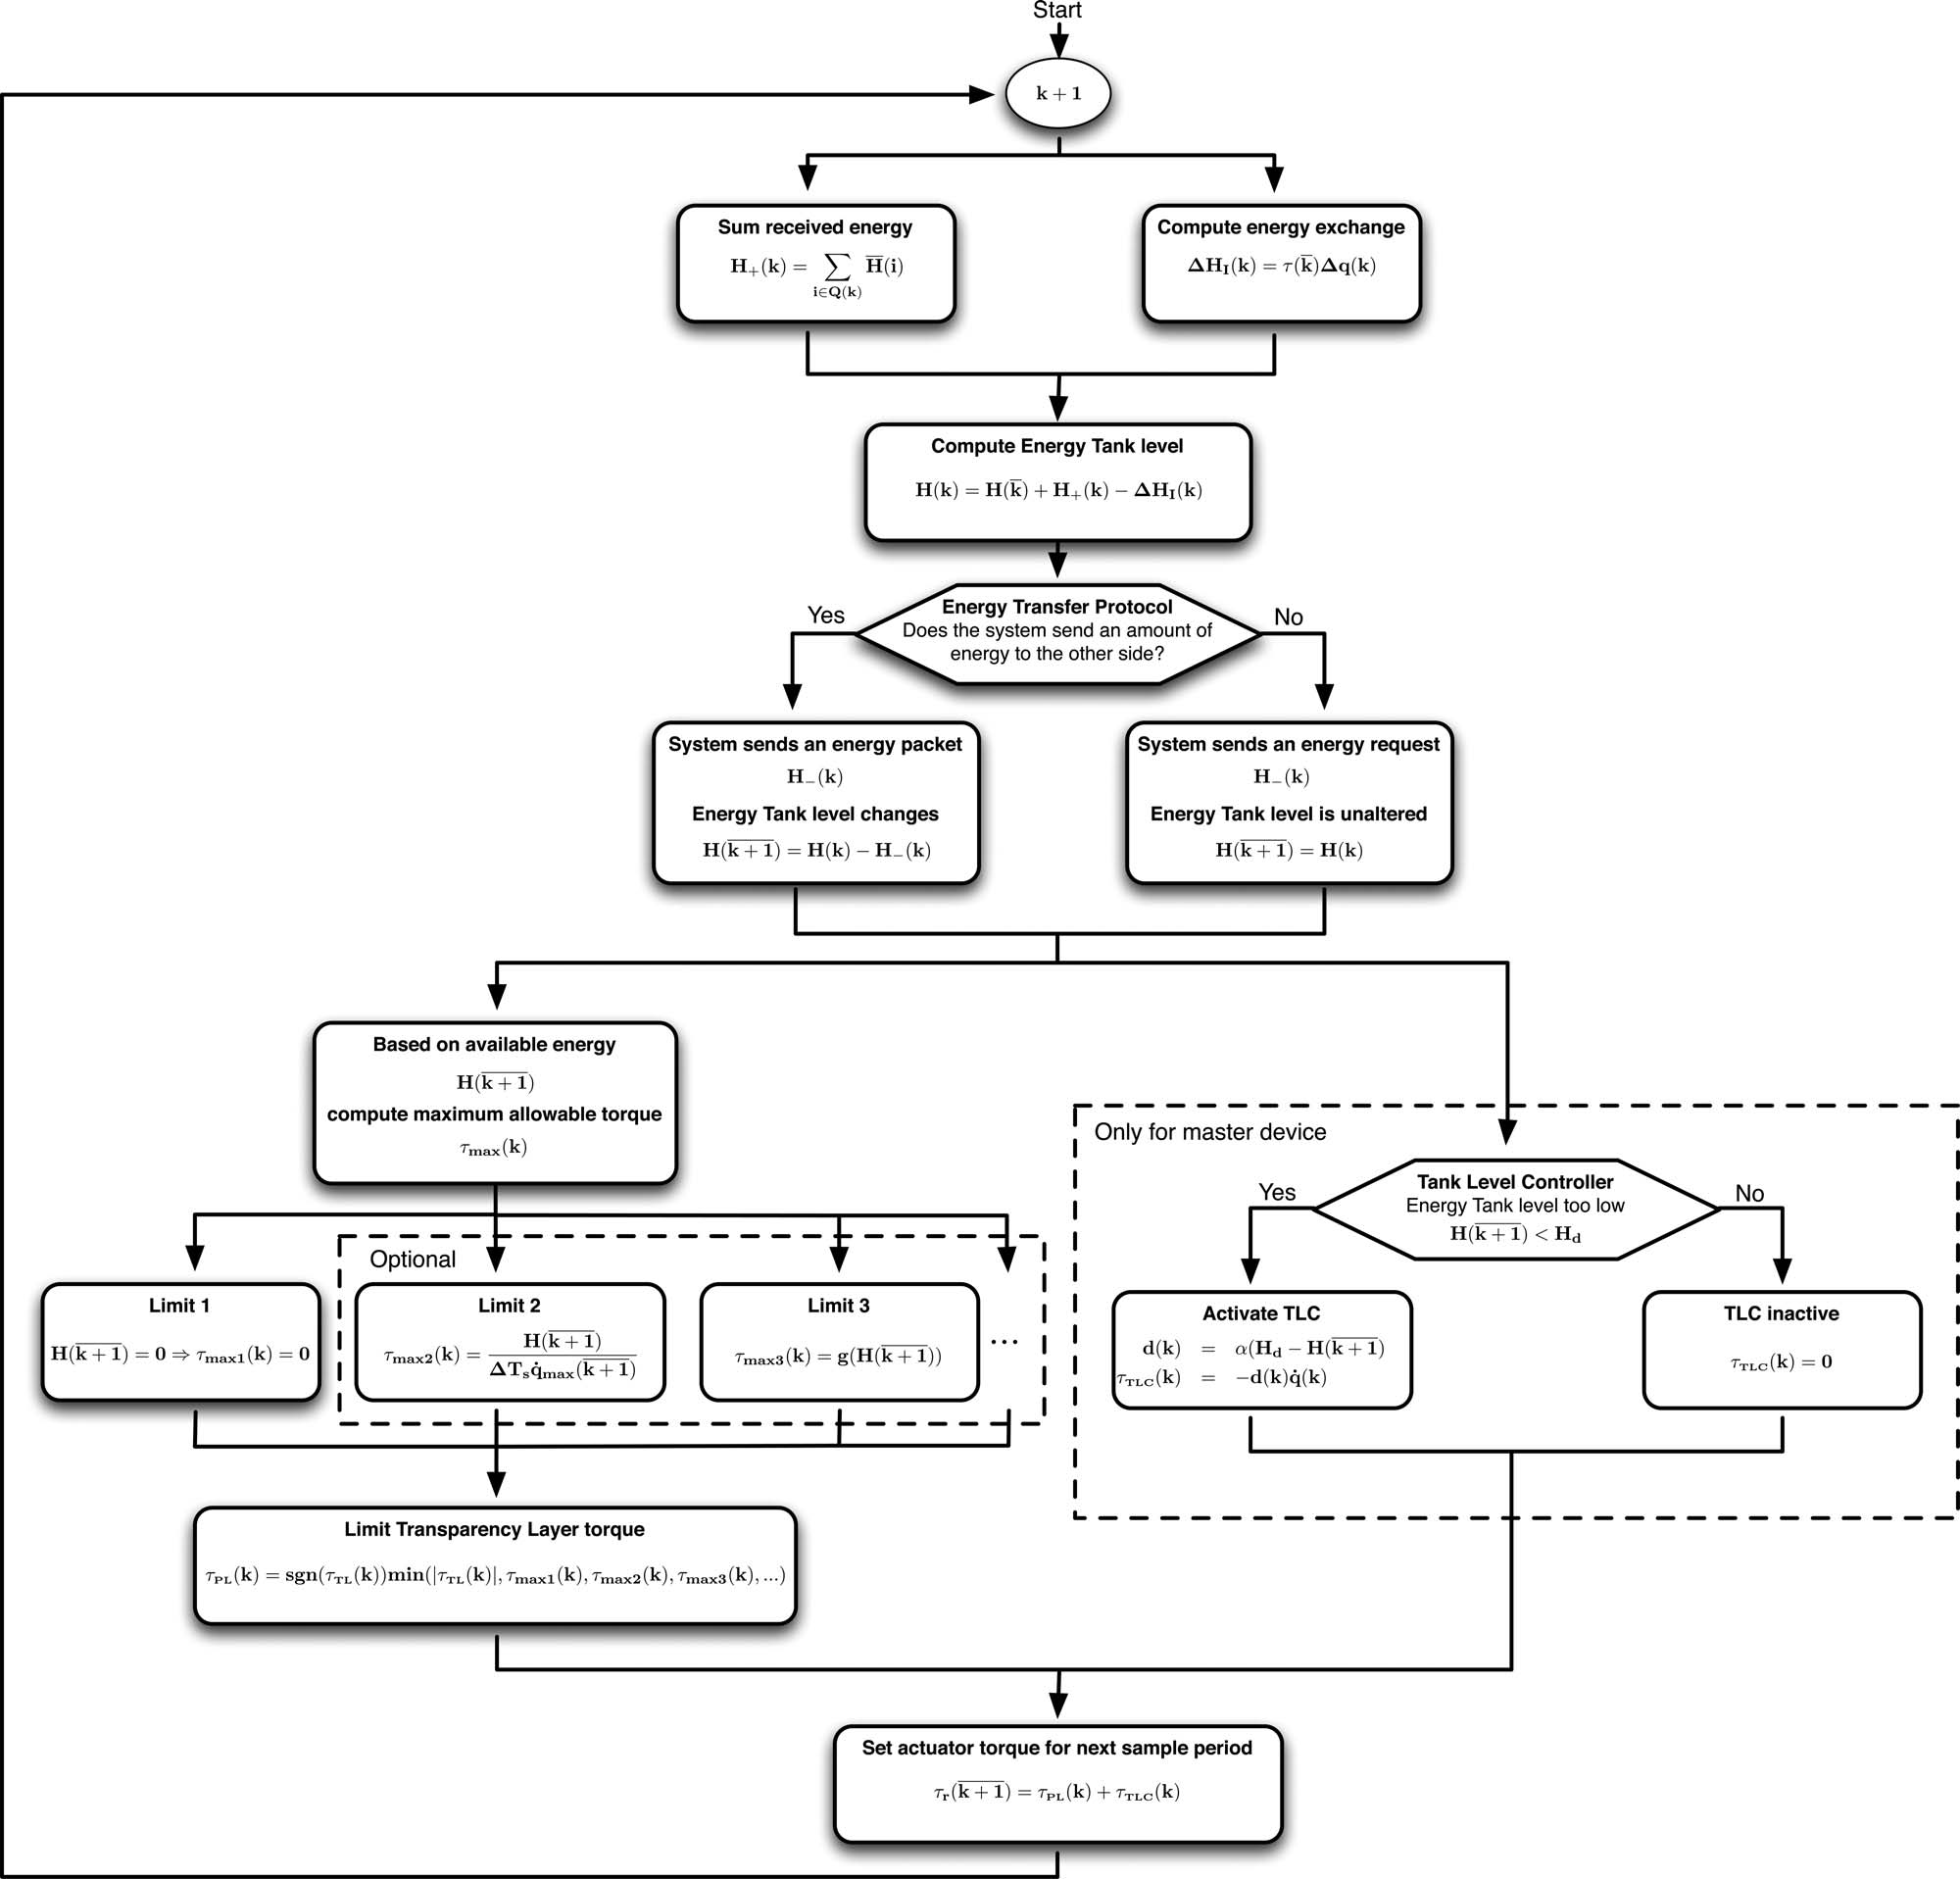
\includegraphics[scale=0.28]{images/architecture.png}
    \end{center}
    \caption{Workflow of the complete passivity layer at either side of the telemanipulation system, taken from \cite{Franken11}}
    \label{fig:architecture}
\end{figure}

For the complete architecture description please refer to \cite{Franken11}.

\subsection{Two-Layer bilateral architecture Force Position}
The idea of the scattering based FP is to use the master velocity as a velocity reference for the slave side and the interaction force with the environment as a reference for the master side. In this scenario the two layer architecture Position-Force was evaluated with a delay of 10 time steps in the communication channel. The environment used is $B_e = 10$ and $K_e = 200$. 

\bigskip
In Figure \ref{fig:energy_pf_free} the free motion response of a sinusoidal reference is reported with proper tuning both at master and slave side.

\begin{figure}[H]
    \begin{center}
        \hspace*{-4.5cm}
        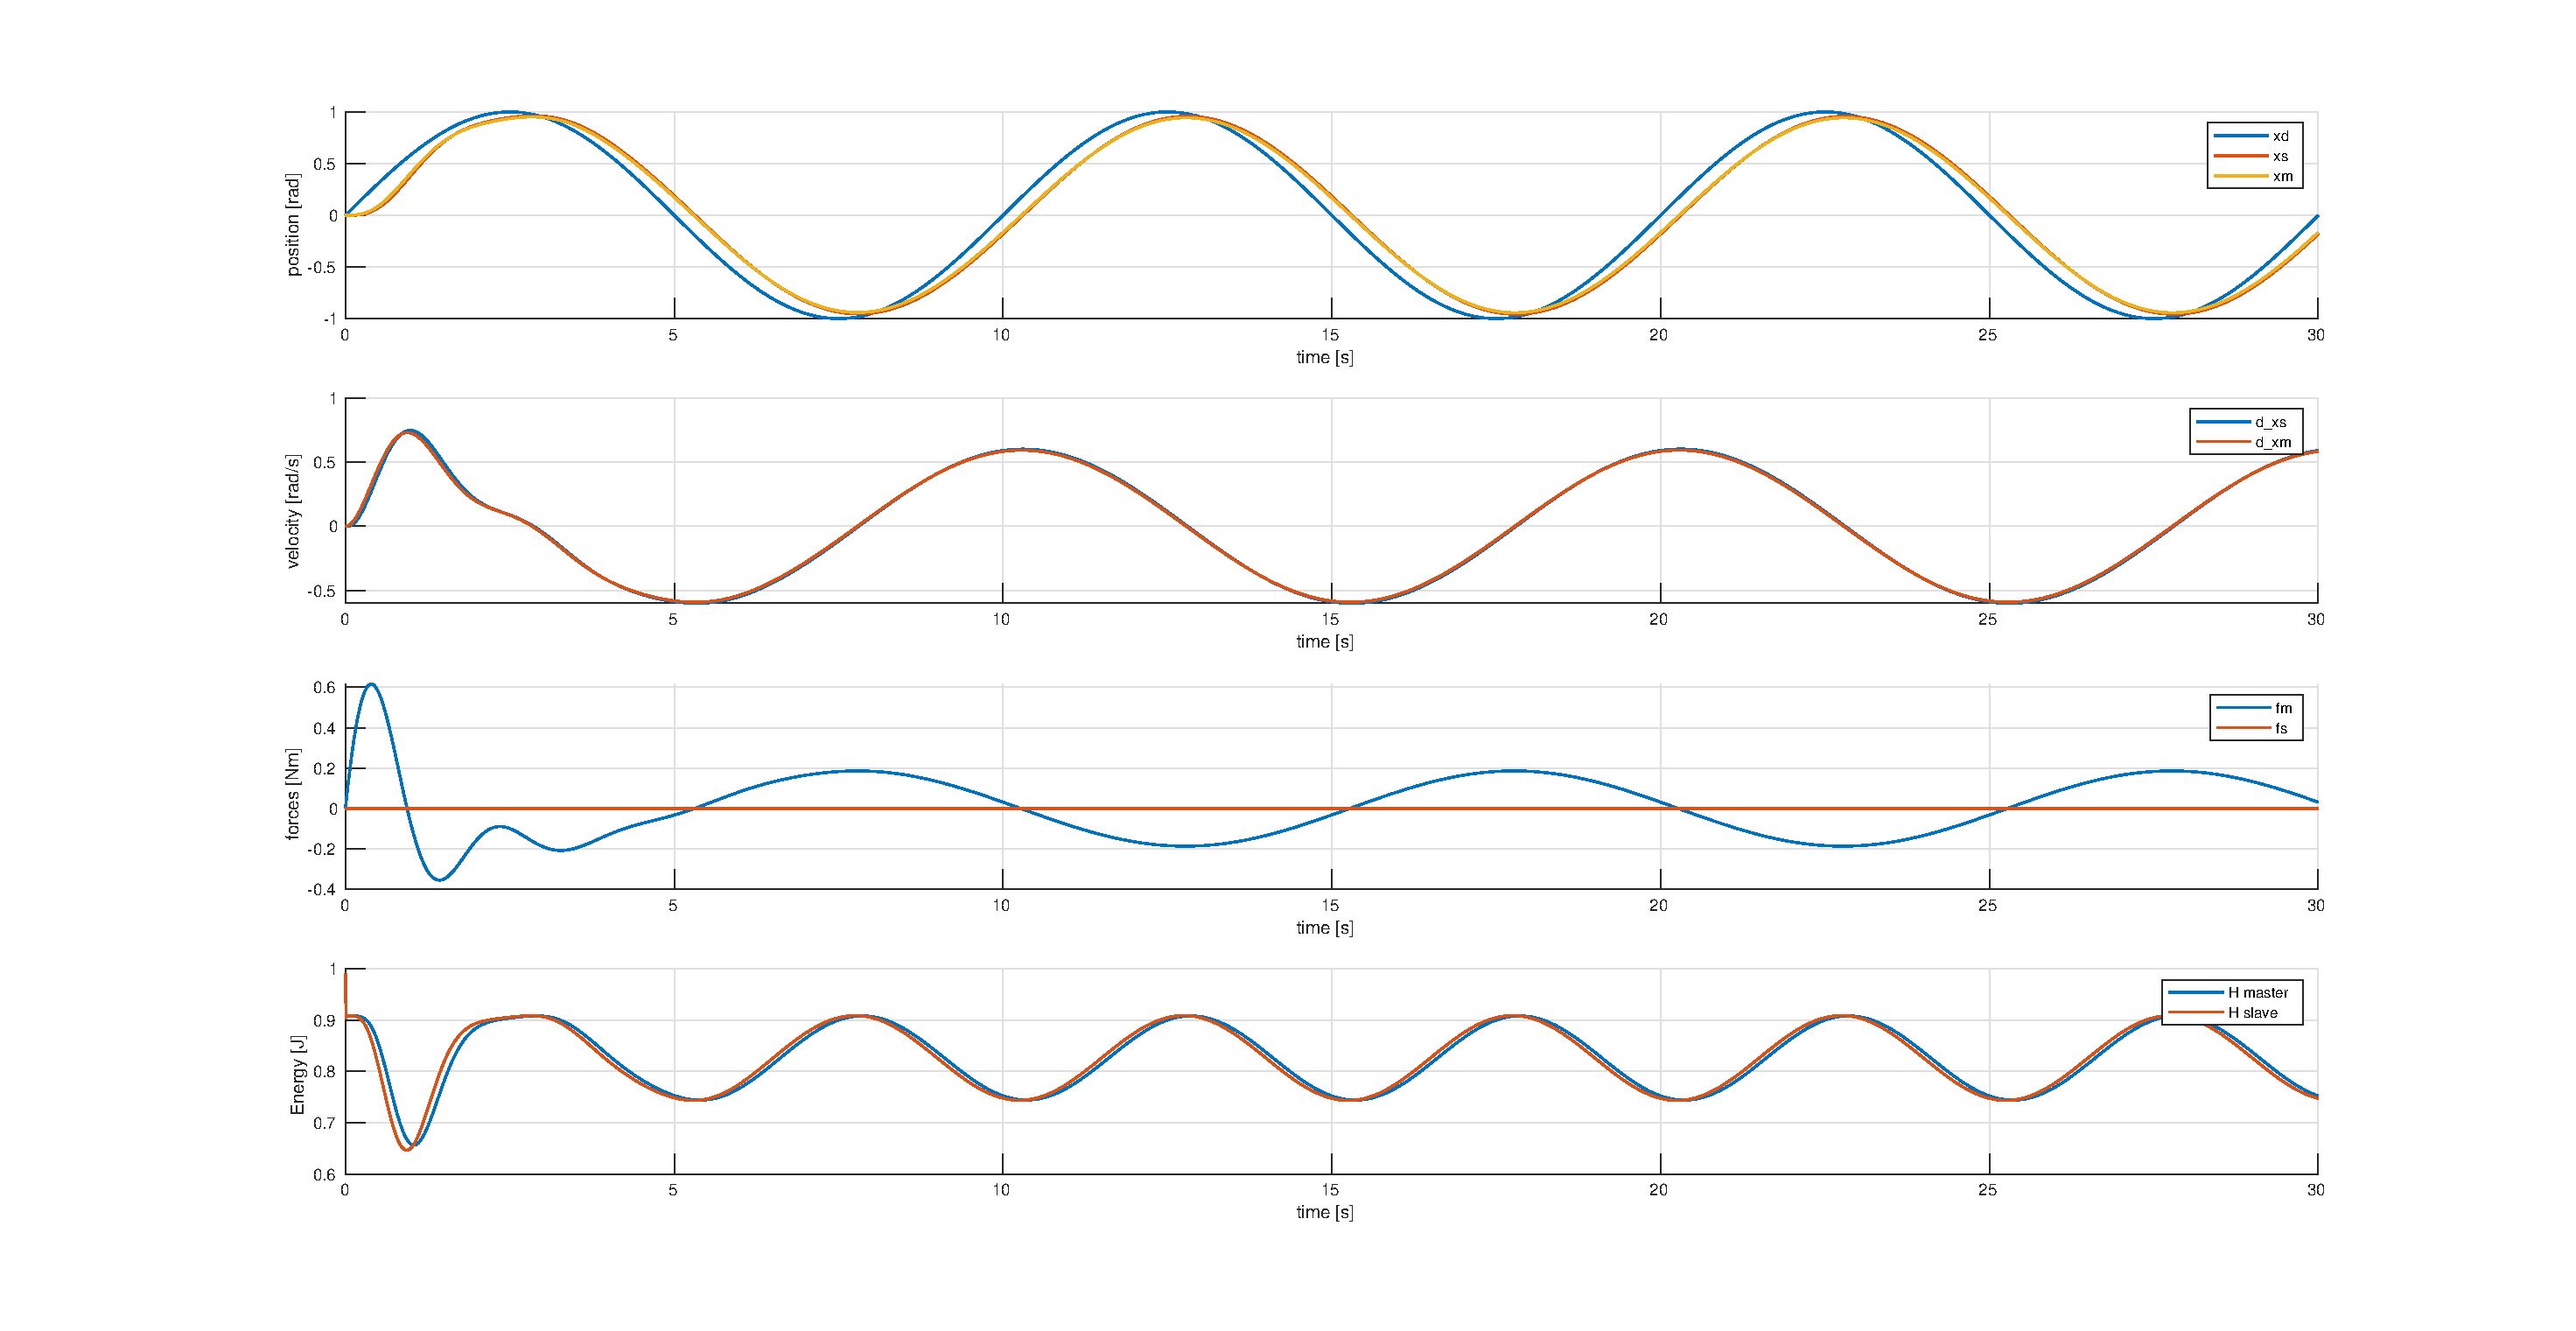
\includegraphics[scale=0.5]{images/energy_pf_free.eps}
    \end{center}
    \caption{Two-Layer bilateral architecture FP in free motion with energy in the tanks}
    \label{fig:energy_pf_free}
\end{figure}

\newpage
In Figure \ref{fig:energy_pf_contact} the contact plot of a sinusoidal reference is reported with proper tuning. Enough initial energy was set in the tanks to perform the task.

\begin{figure}[H]
    \begin{center}
        \hspace*{-4.5cm}
        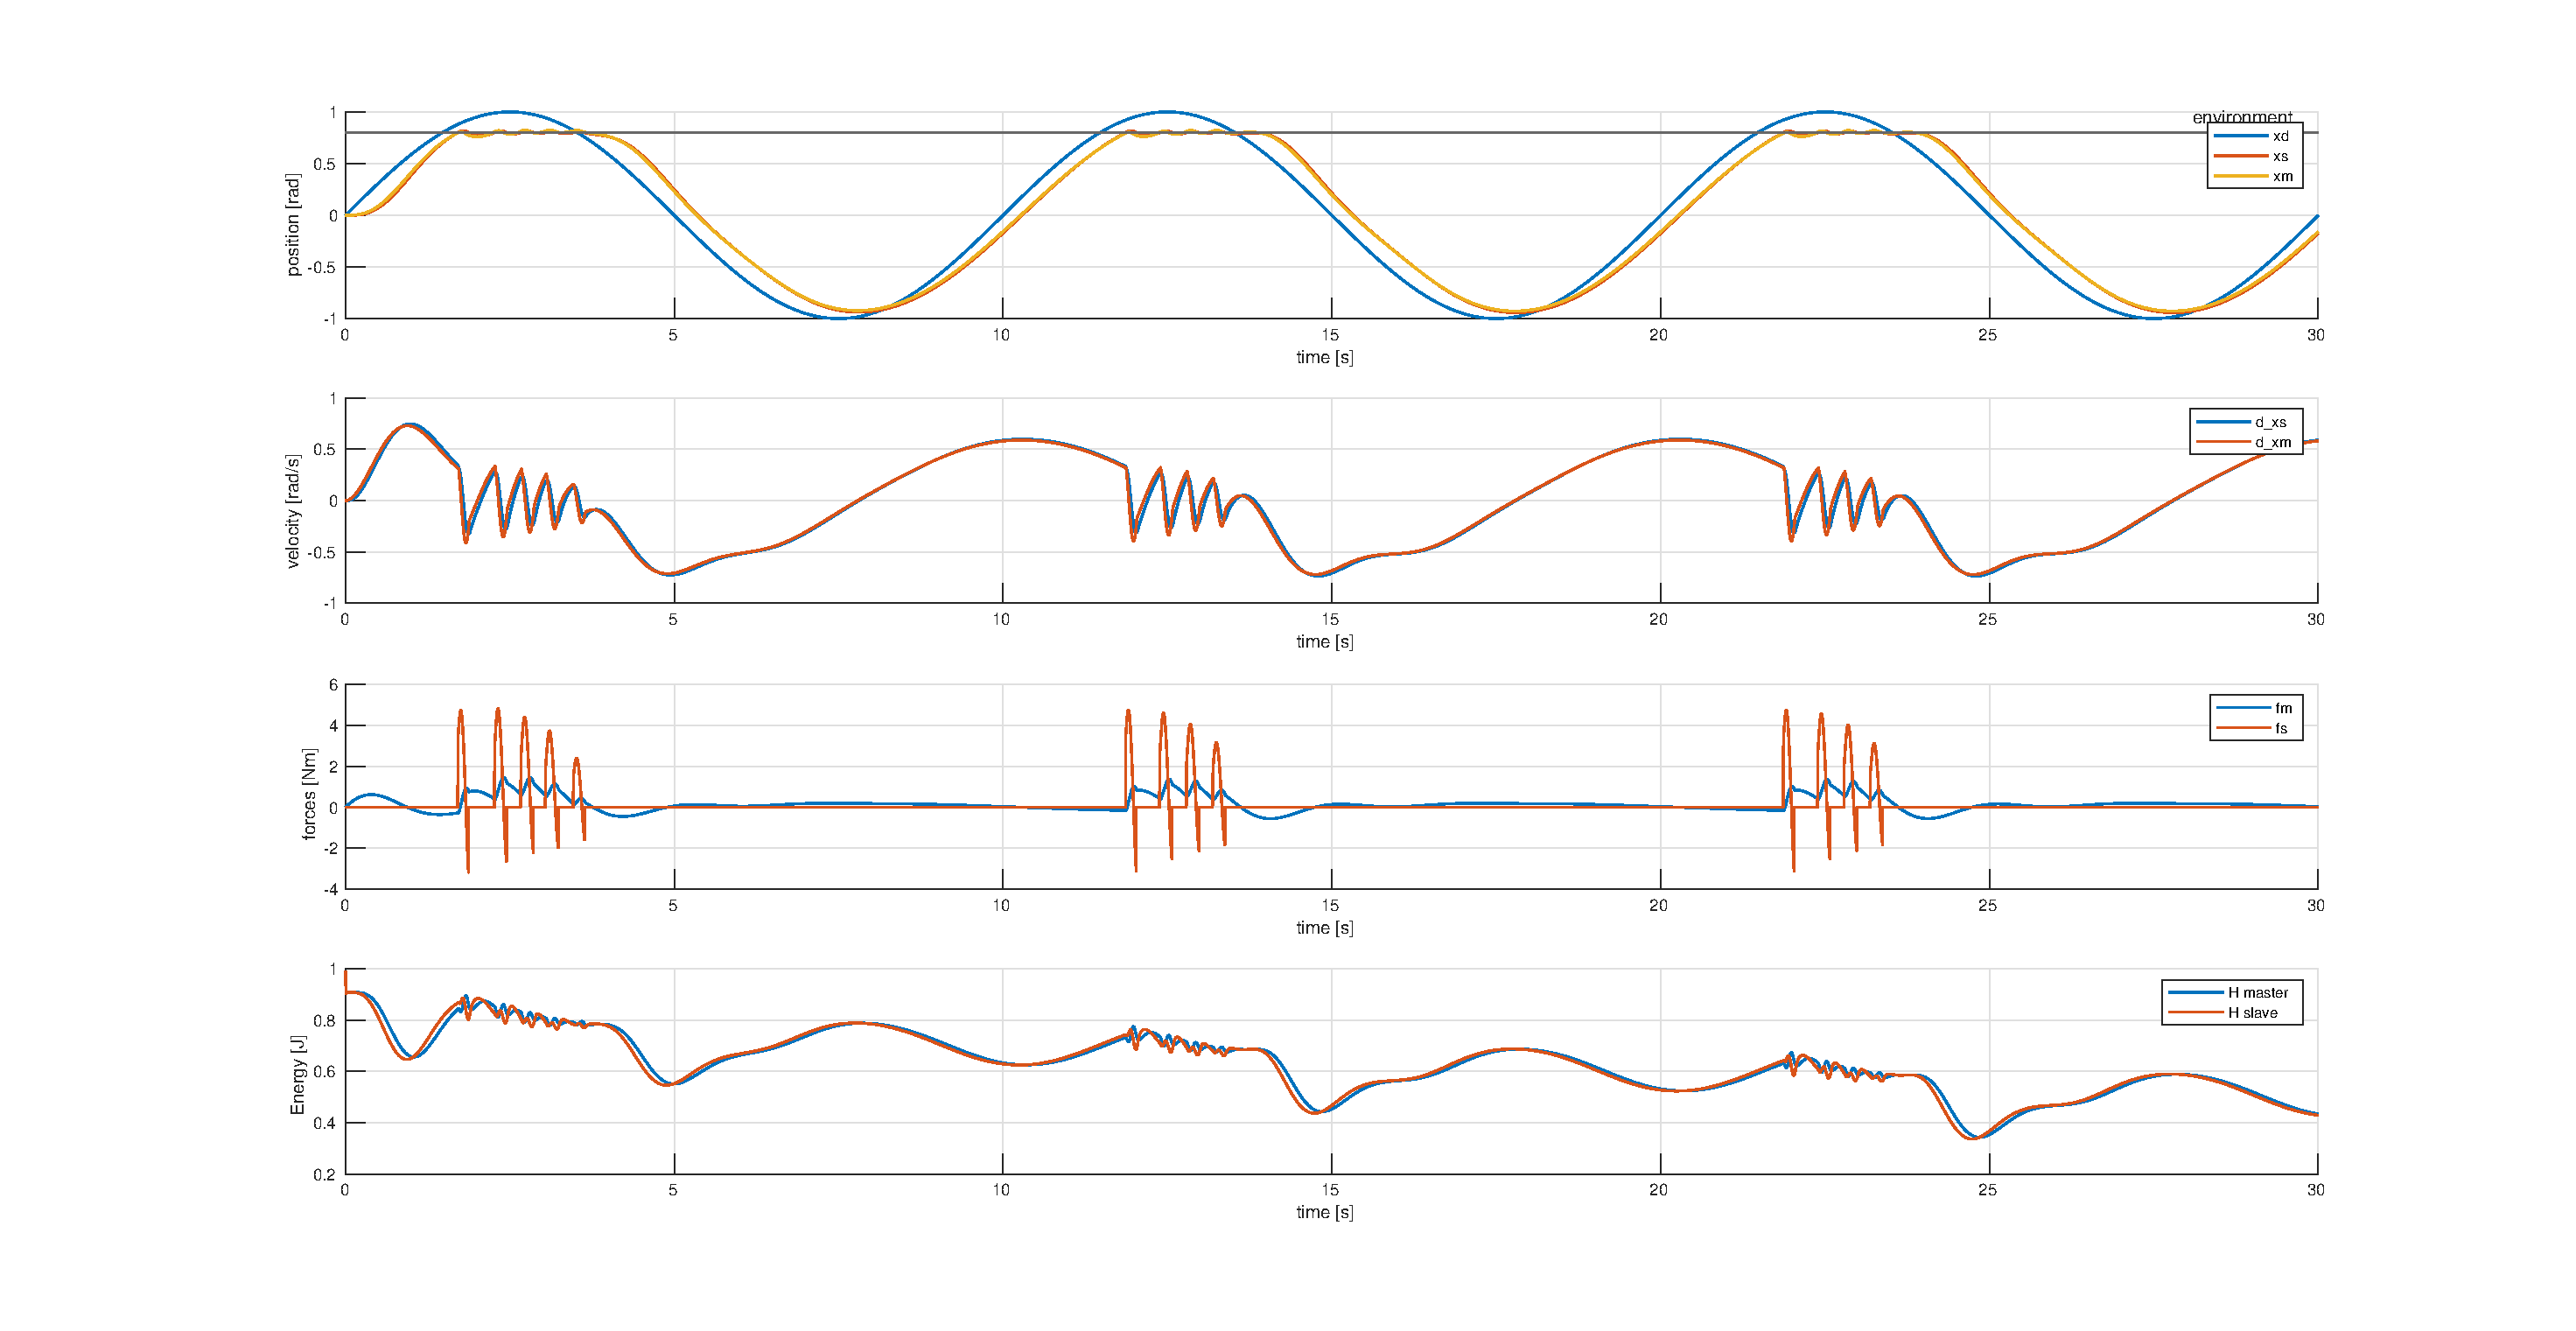
\includegraphics[scale=0.5]{images/energy_pf_contact.eps}
    \end{center}
    \caption{Two-Layer bilateral architecture FP in contact at 0.8}
    \label{fig:energy_pf_contact}
\end{figure}

The parameters used for the energy layer are $\alpha = 0.1$, $\beta = 0.01$ and the level for the TLC $H_d = 0.5$. However this values are indicative and were briefly adjusted in the various scenarios to obtain the related plots.
\bigskip

In Fig \ref{fig:energy_pf_no_energy} the actual effect of the passivity layer is reported when there is no initial energy. The passivity layer actually modulates the transparency command due to missing energy.

\begin{figure}[H]
    \hspace*{-4.5cm}
    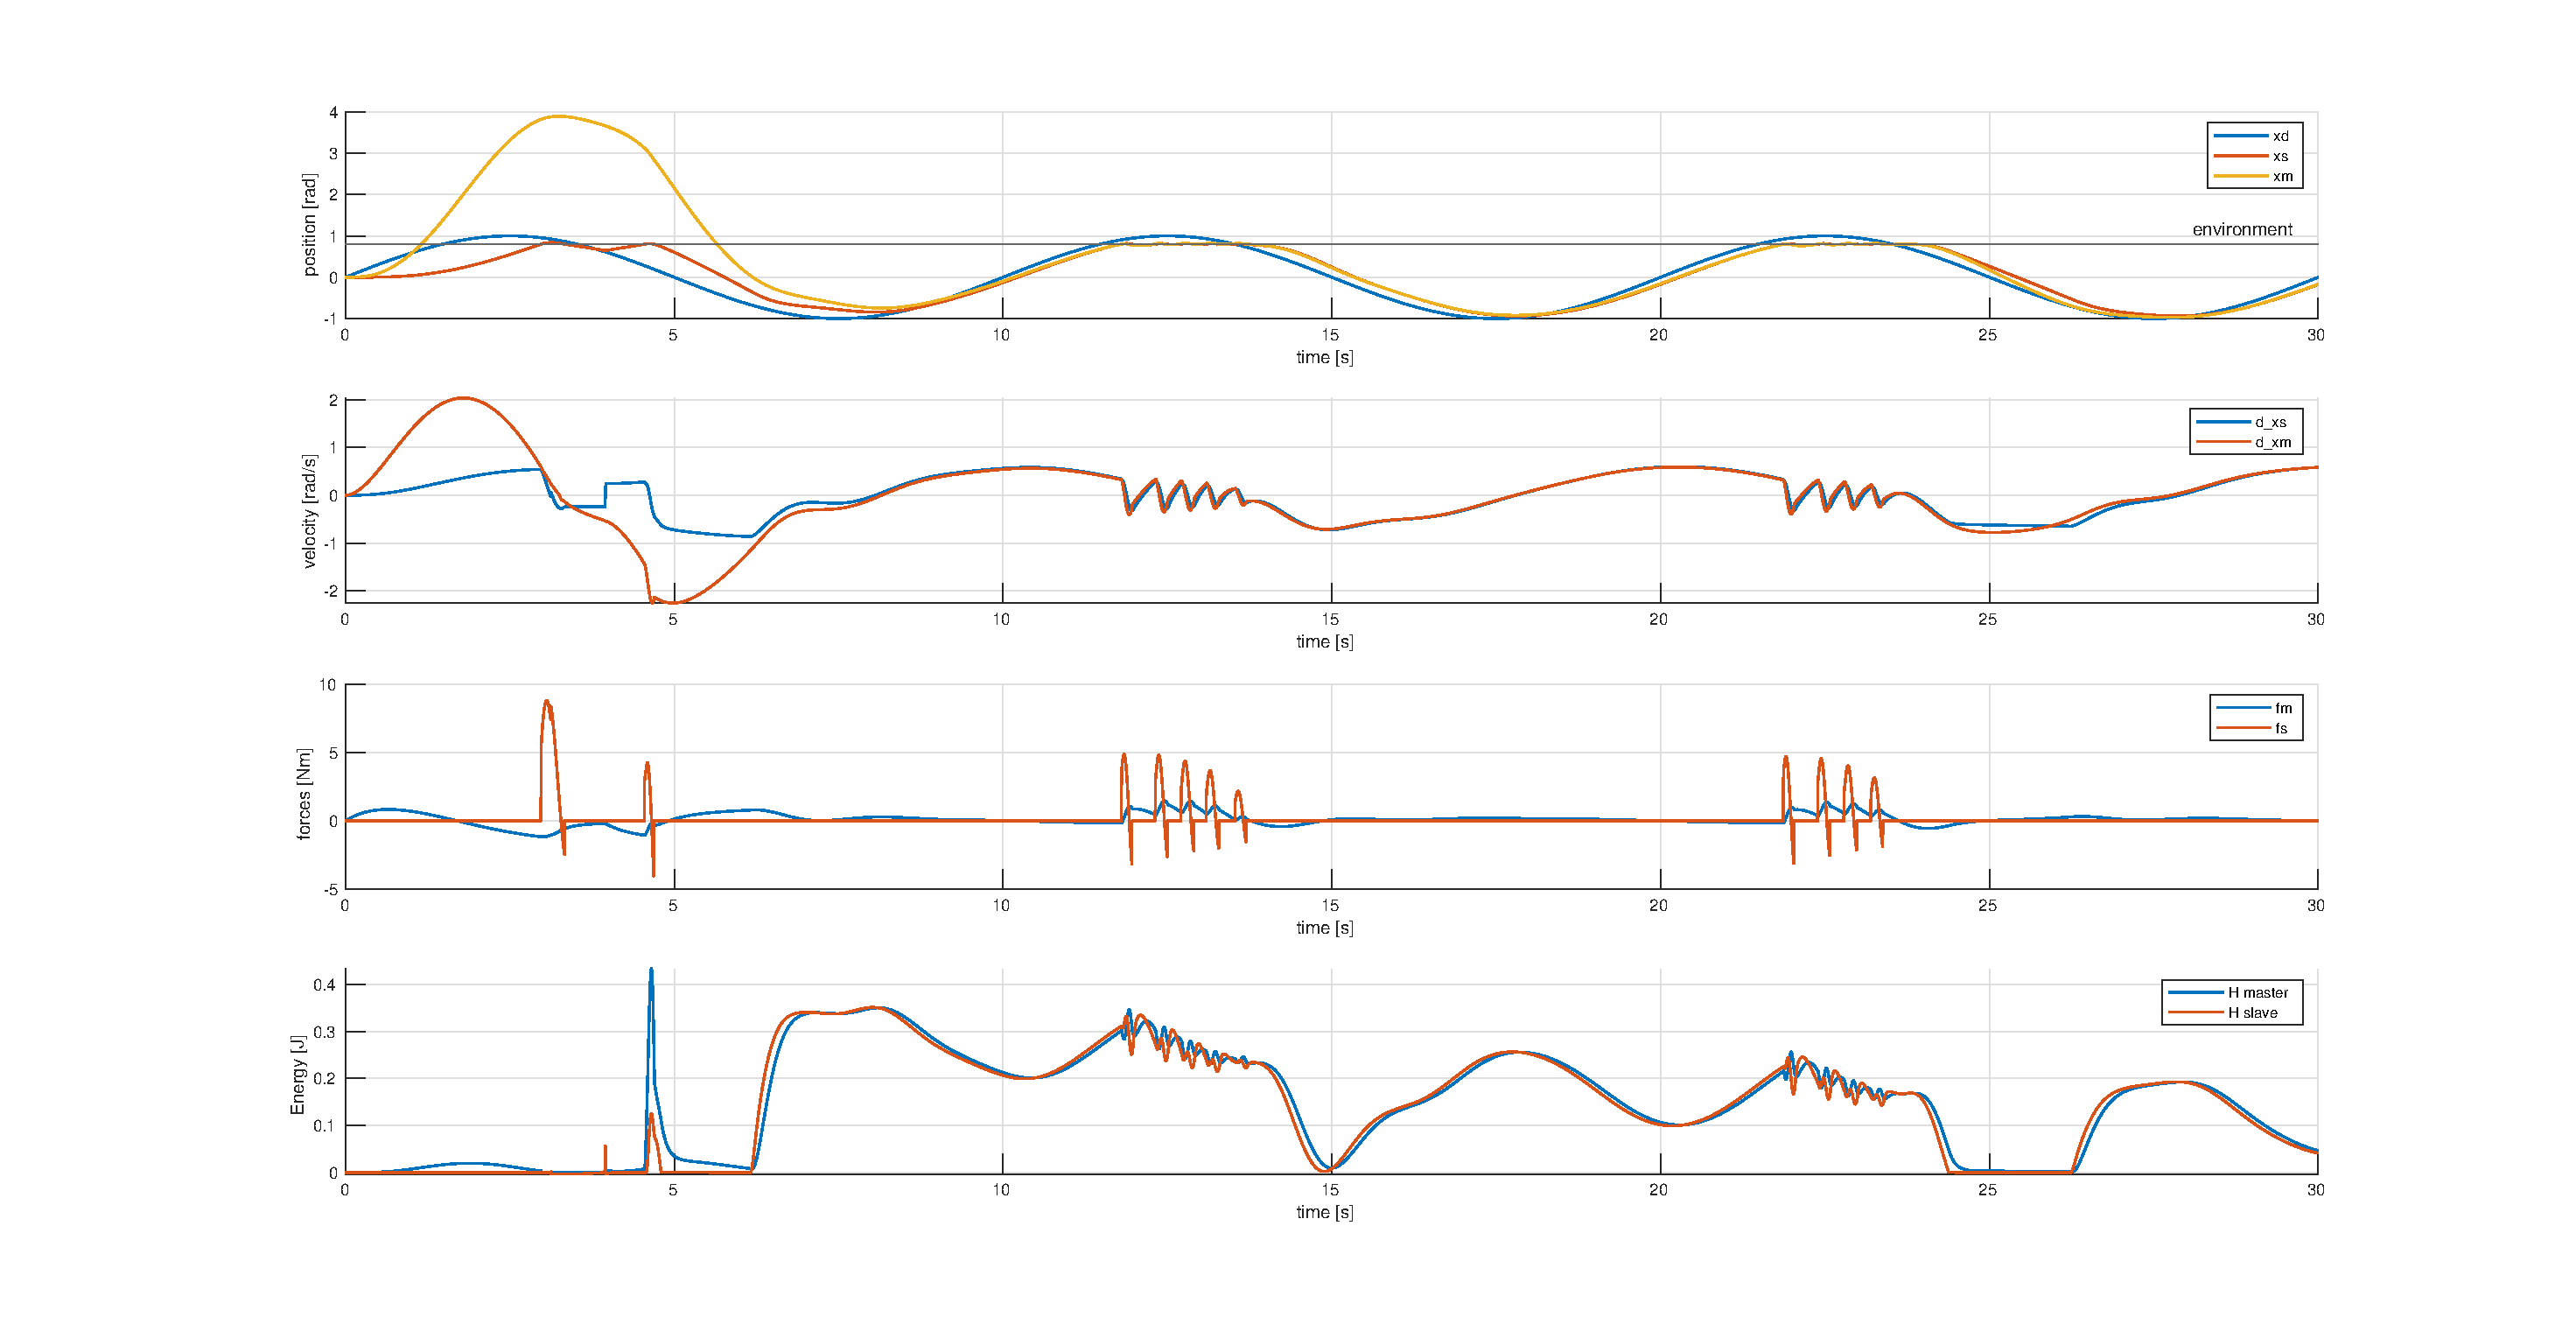
\includegraphics[scale=0.5]{images/energy_pf_no_energy.eps}
    \qquad
    \hspace*{-1.5cm}
    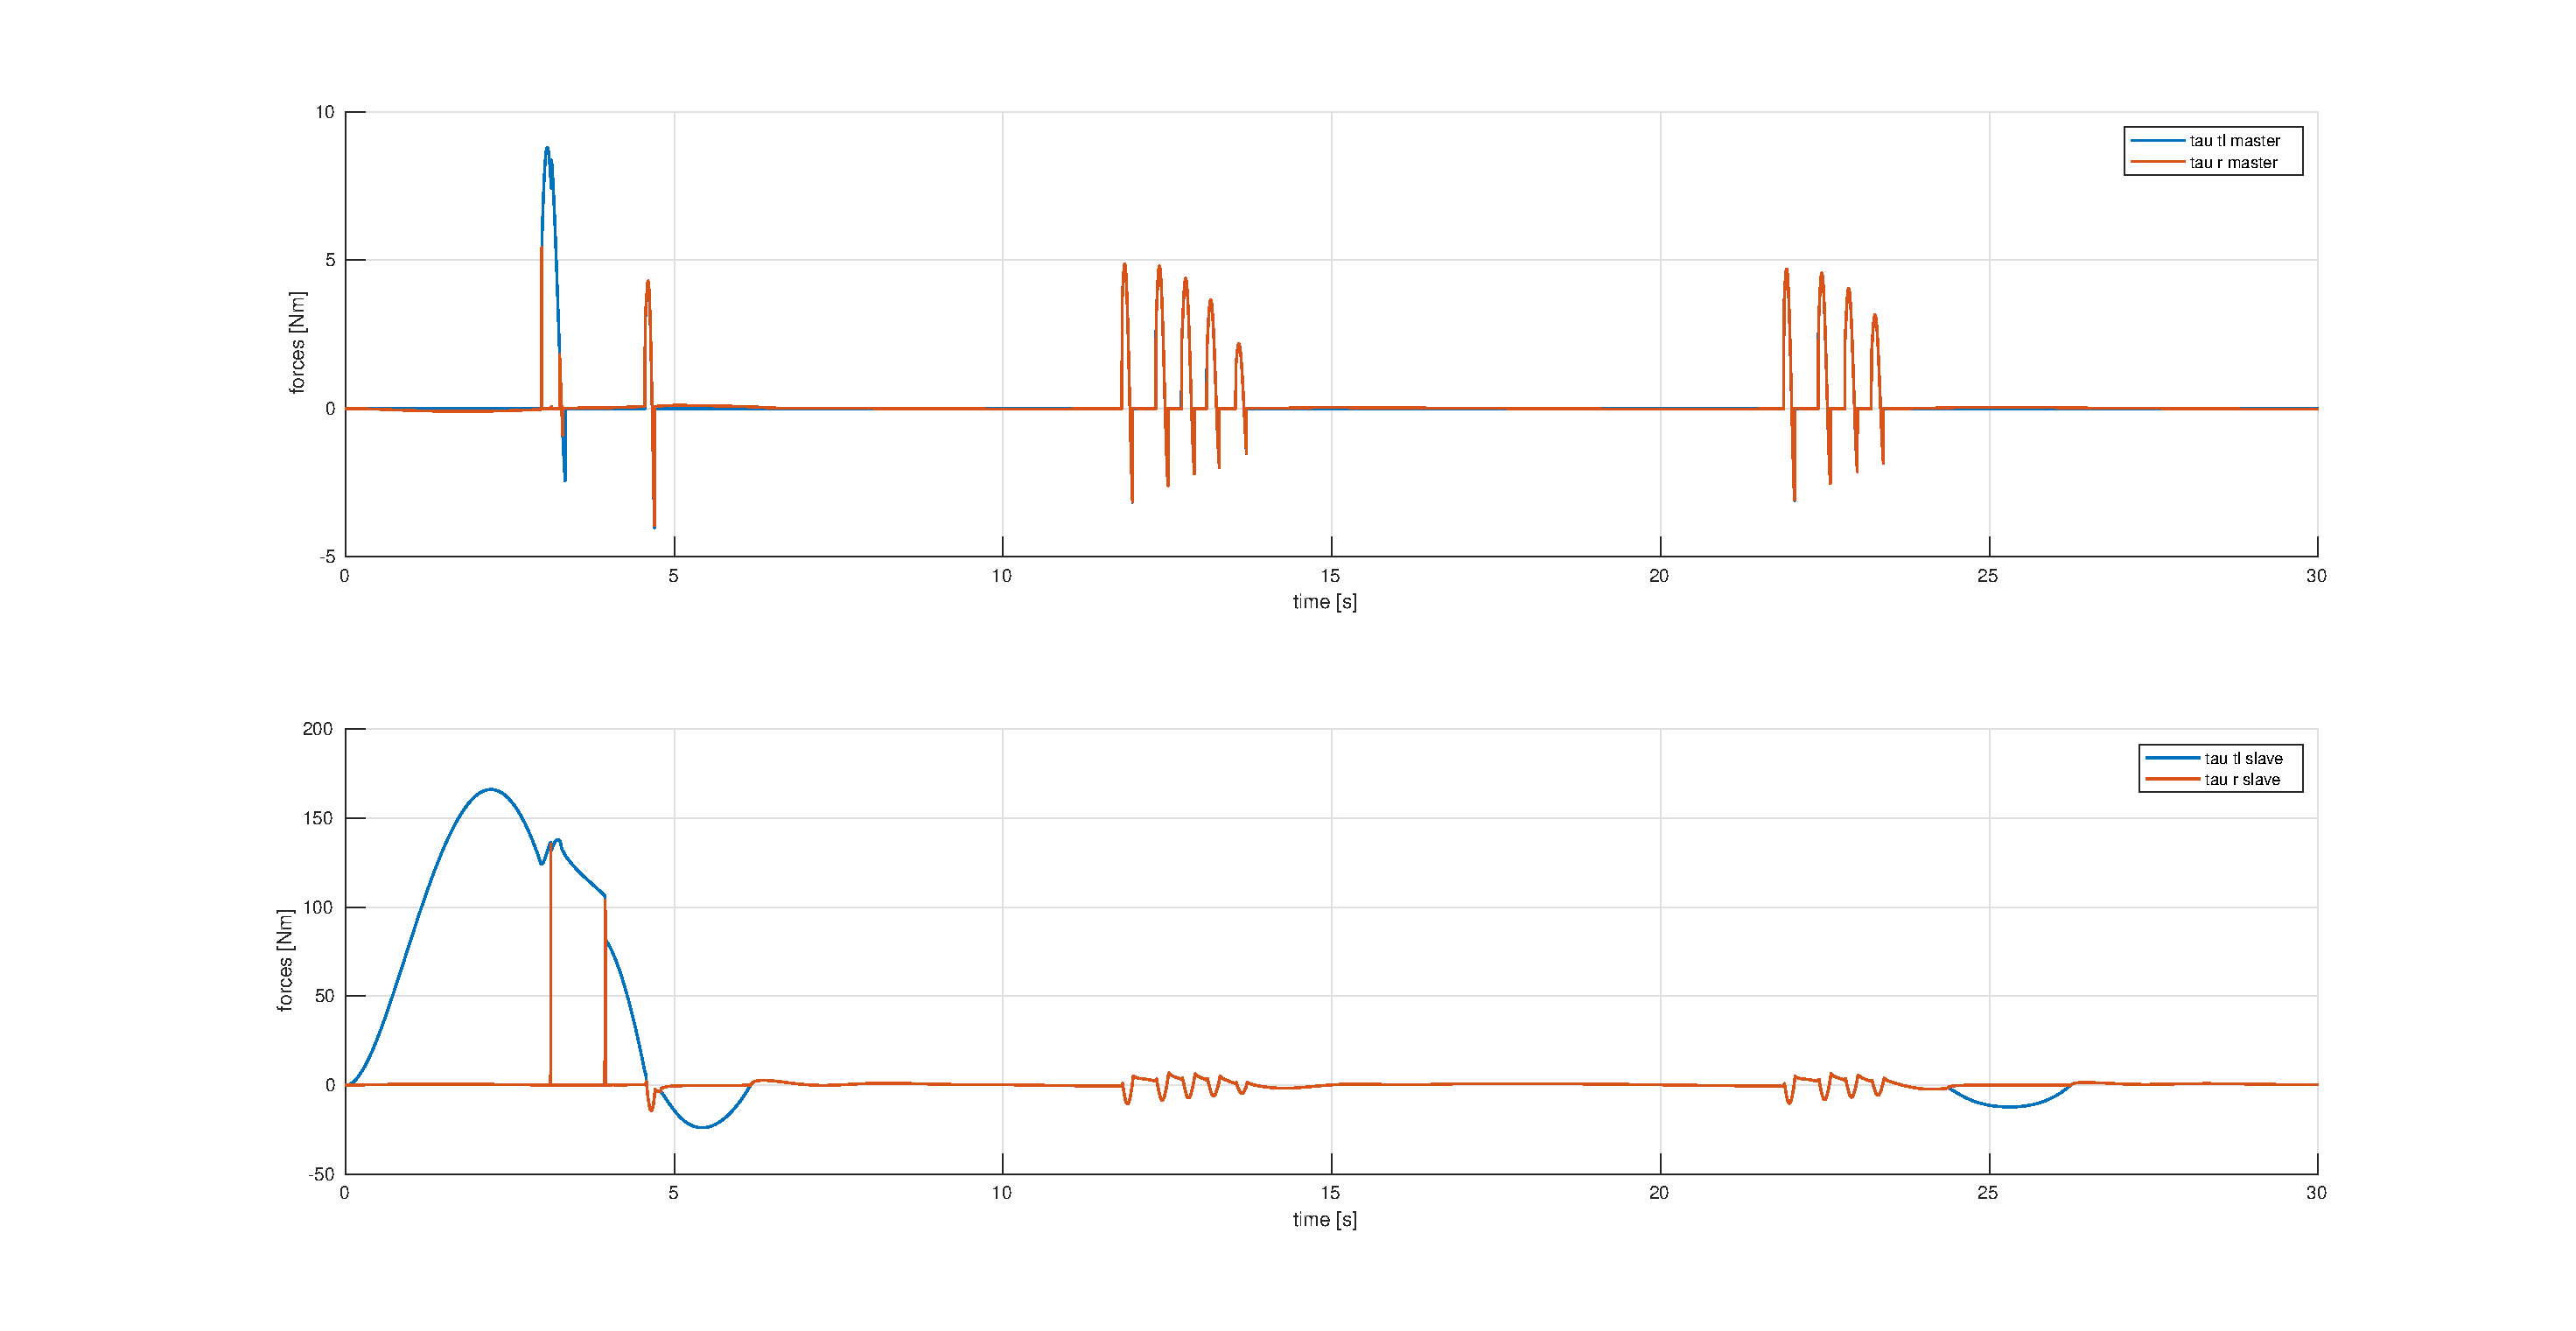
\includegraphics[scale=0.4]{images/energy_pf_tau.eps}
    \caption{Top: Two-Layer bilateral architecture FP in contact at 0.8 with no initial energies. Bottom: Comparison of the torques produced by the transparency and the passivity layer without initial energy in the tanks}
    \label{fig:energy_pf_no_energy}
\end{figure}


\begin{figure}[H]
    \hspace*{-4.5cm}
    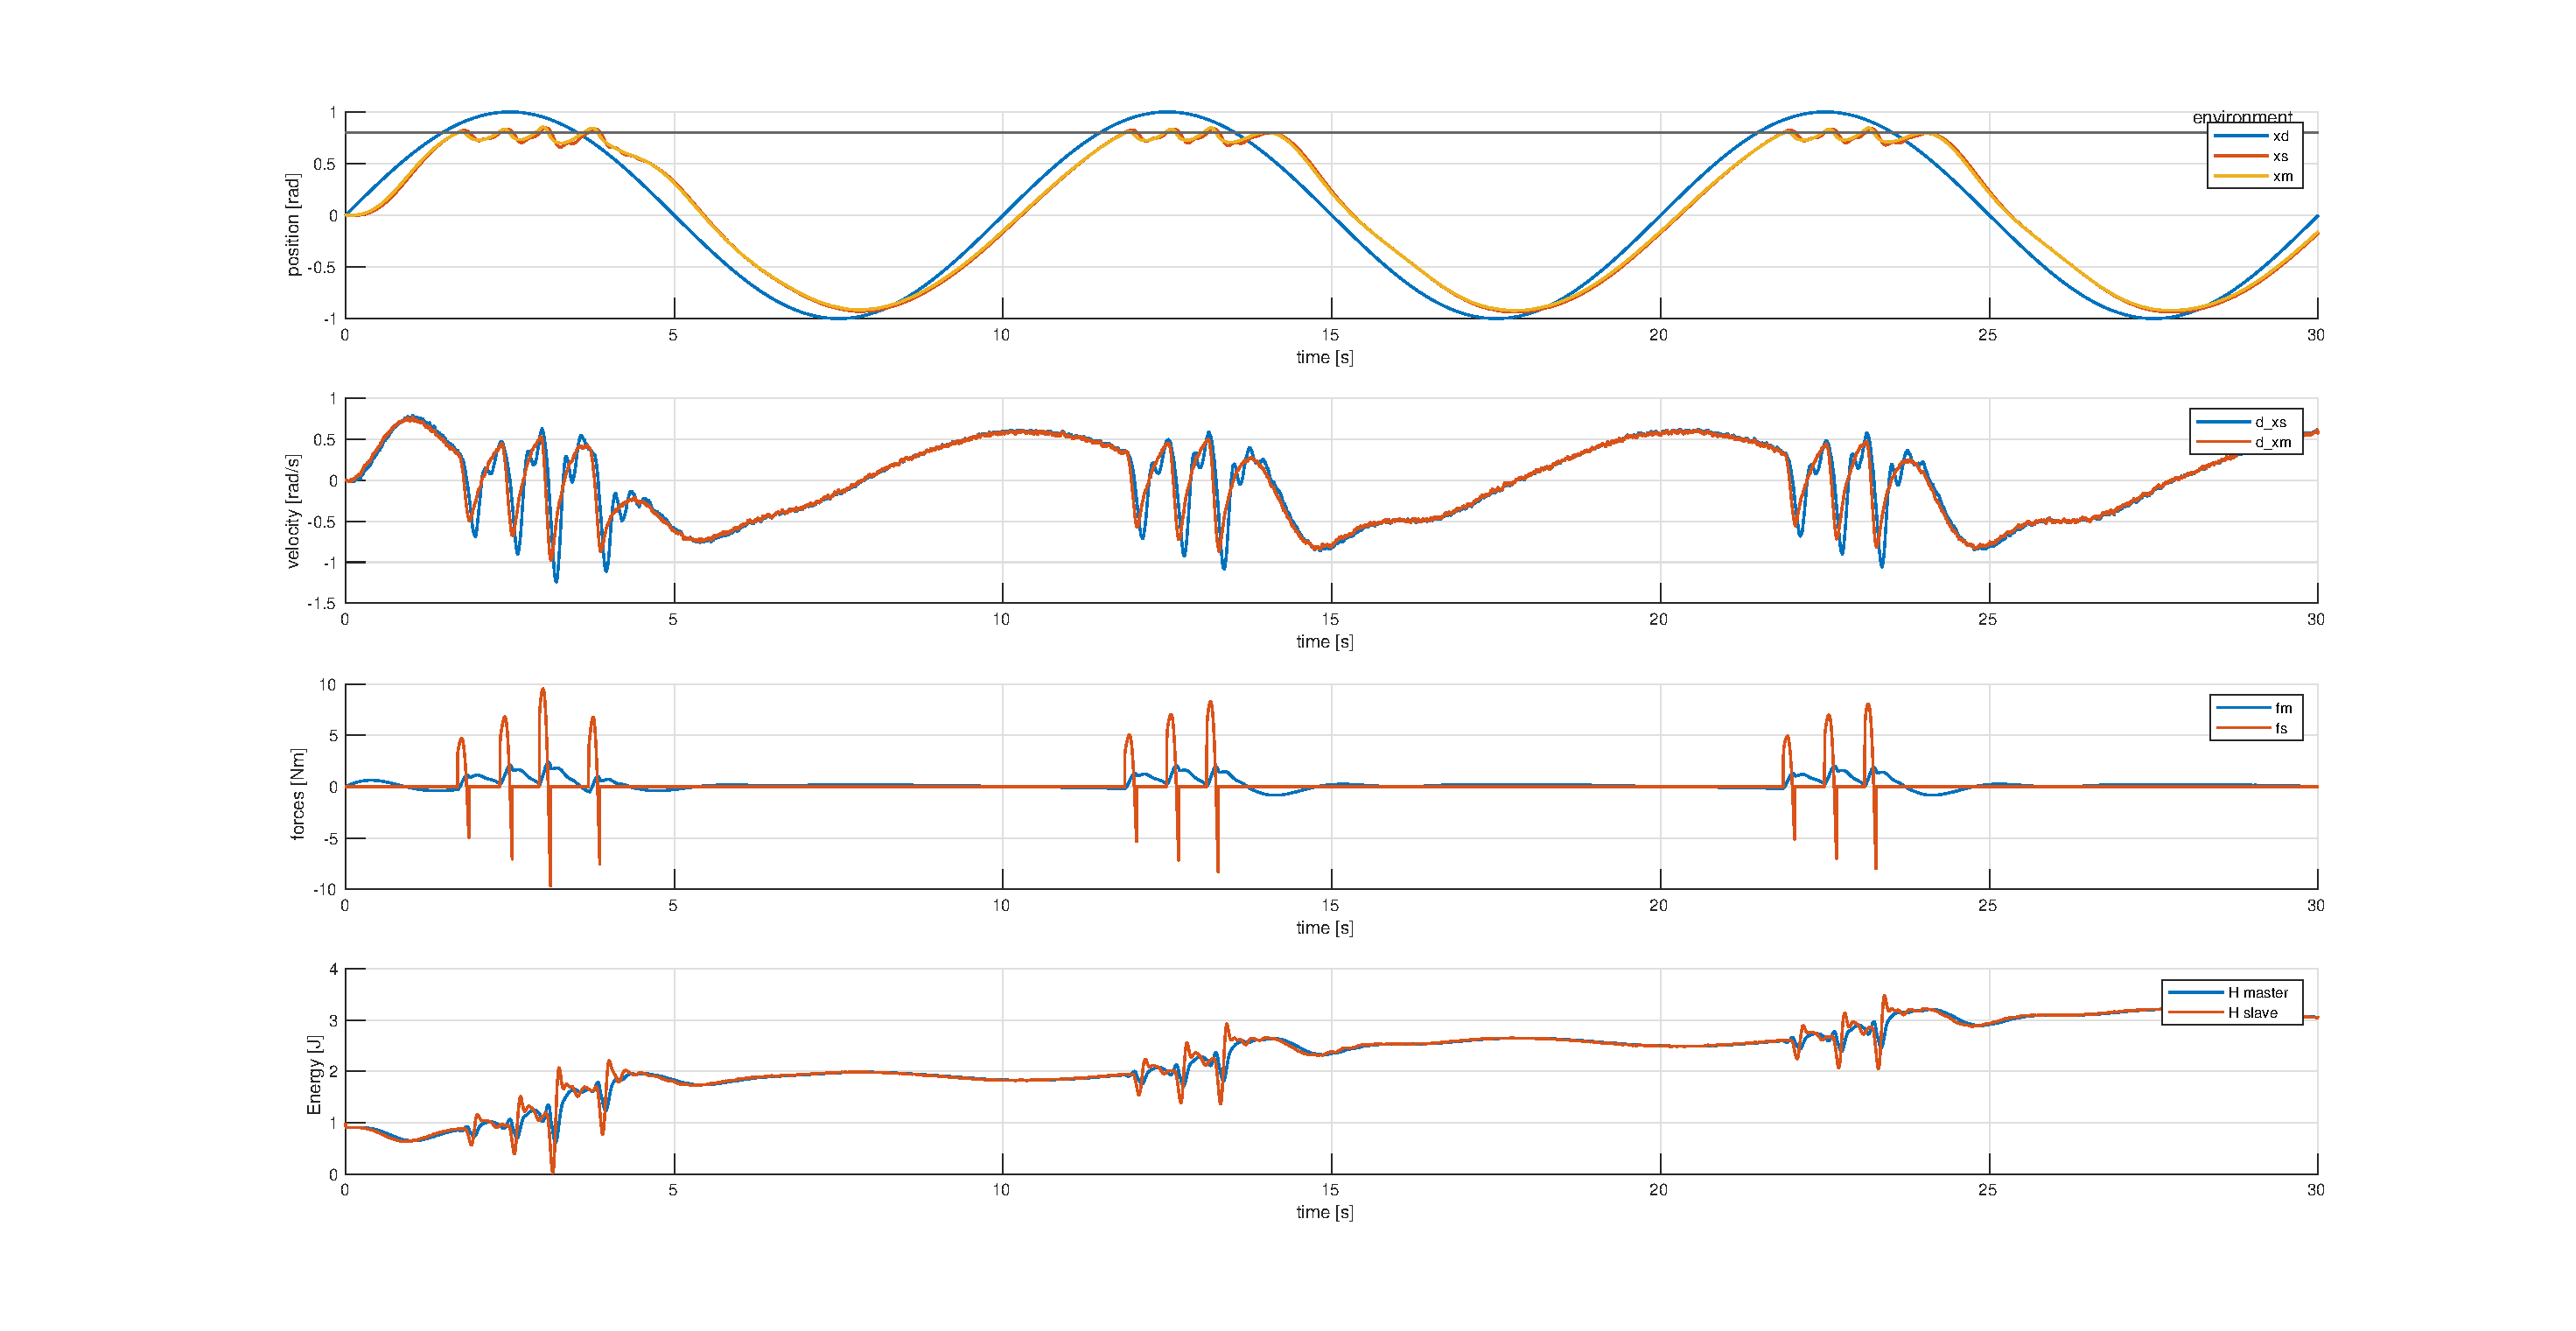
\includegraphics[scale=0.5]{images/energy_pf_kalman.eps}
    \qquad
    \hspace*{-1.5cm}
    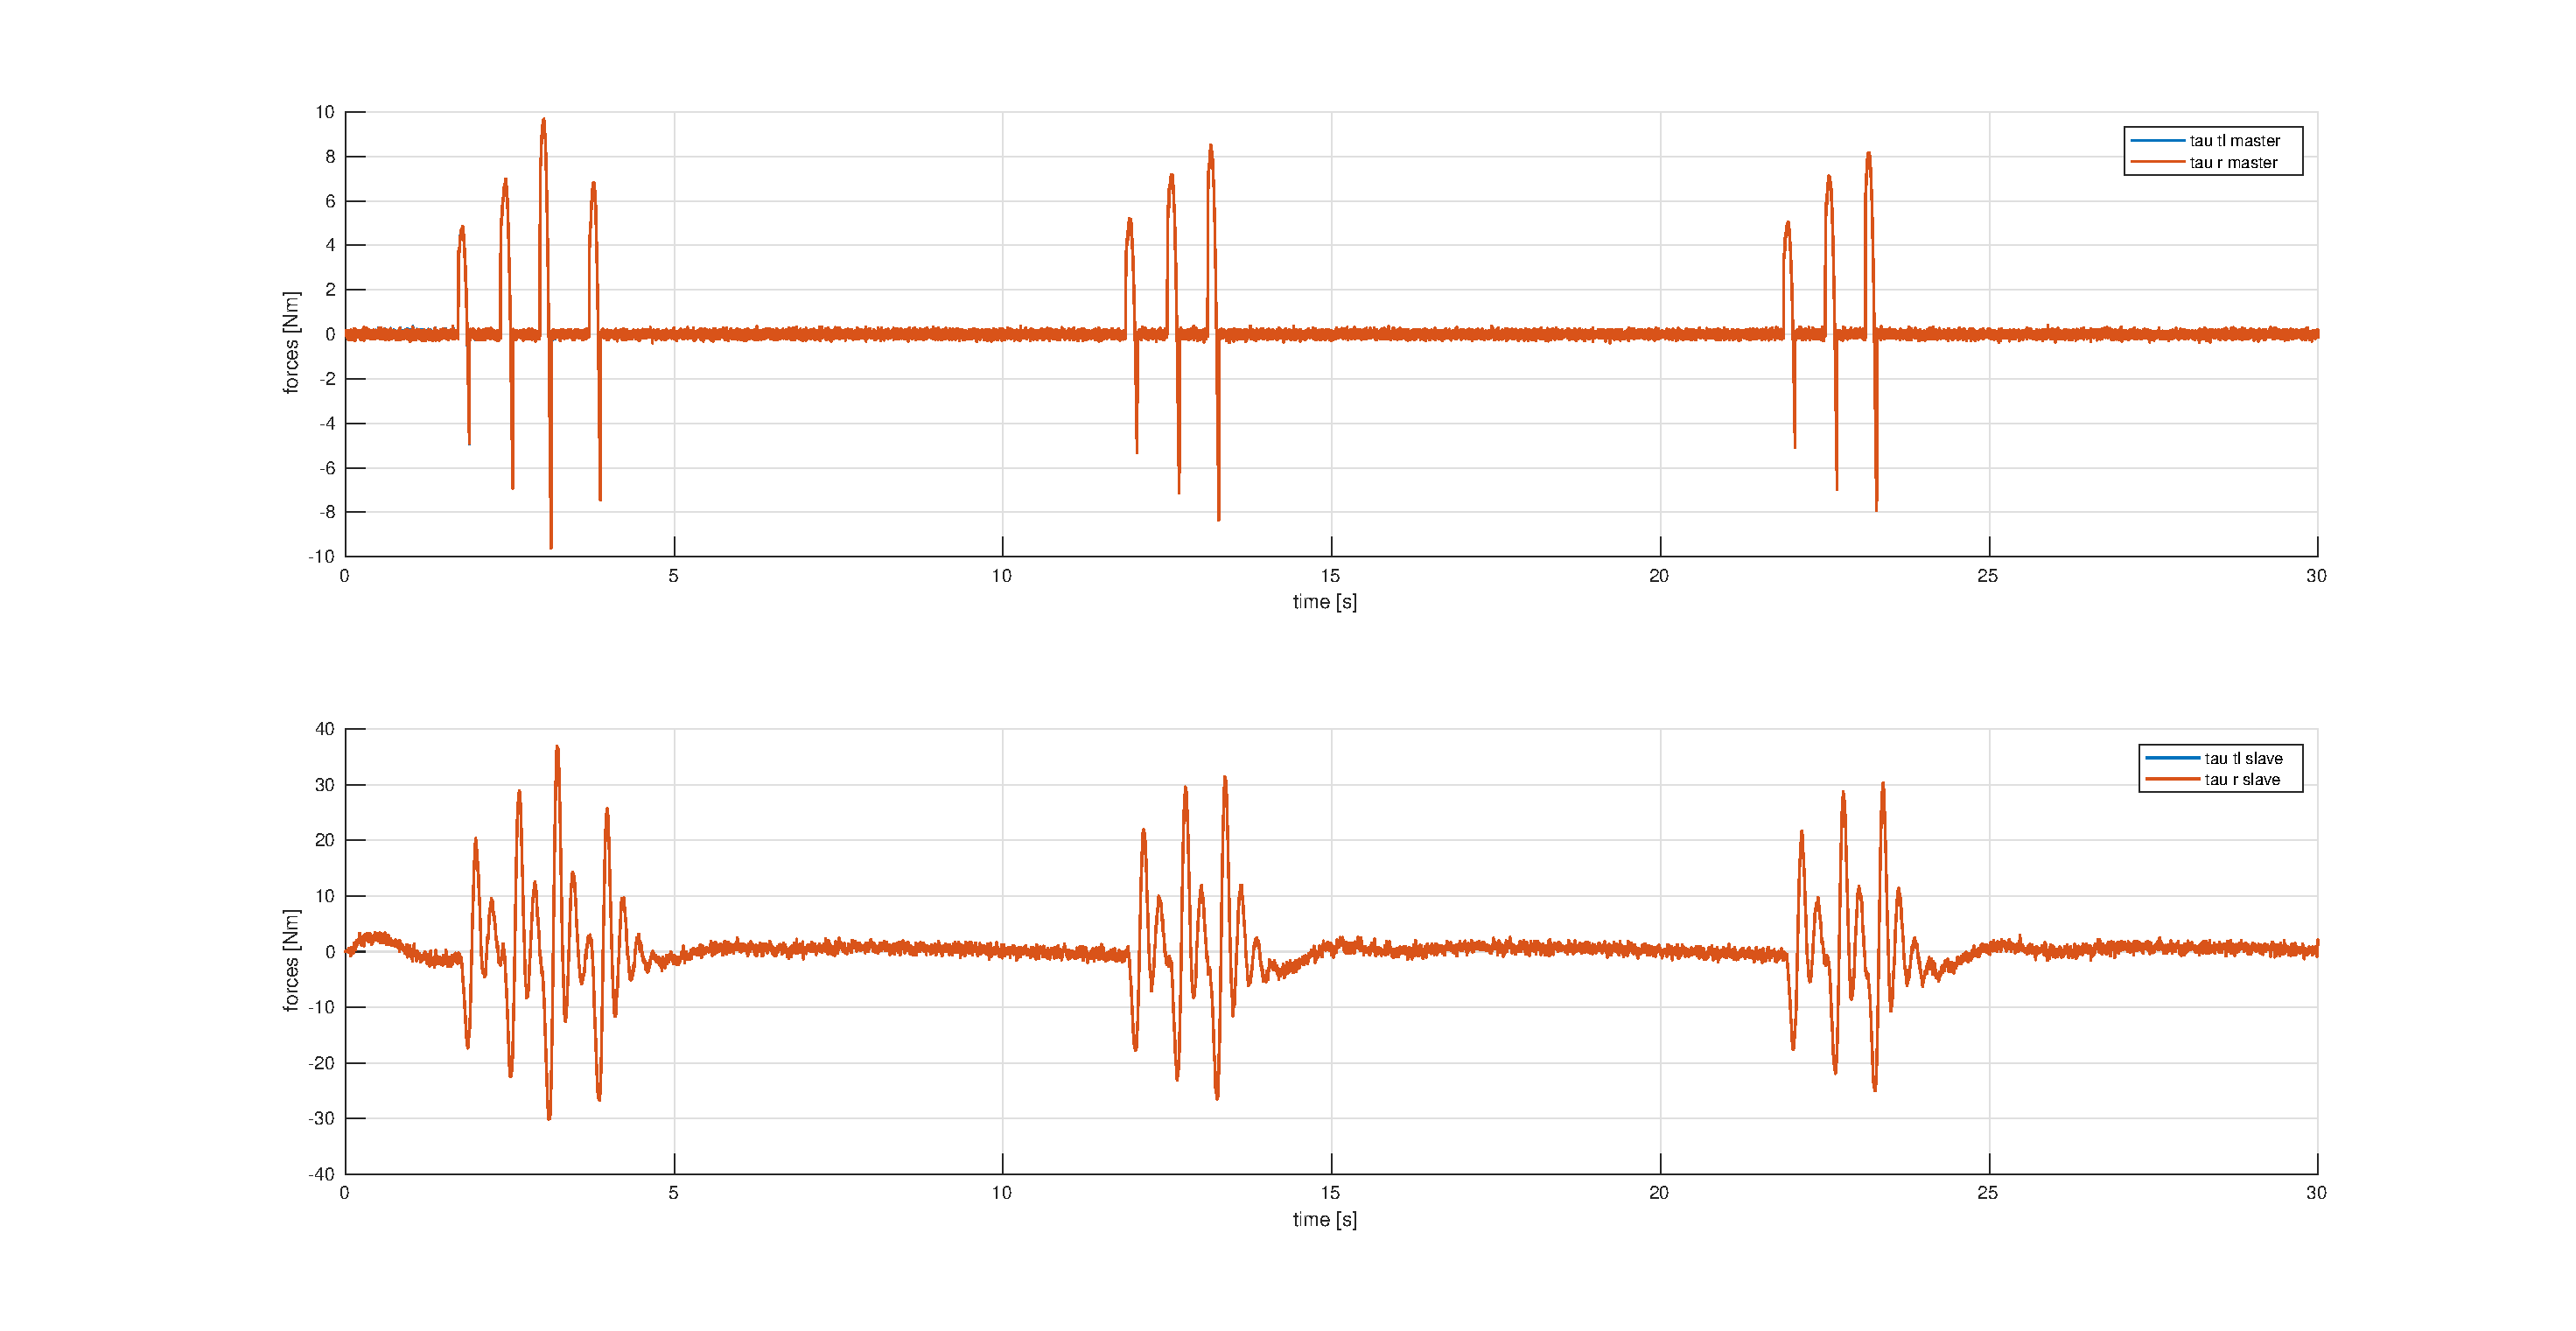
\includegraphics[scale=0.4]{images/energy_pf_tau_kalman.eps}
    \caption{Top: Two-Layer architecture FP in contact at 0.8 with kalman filters. Bottom: Comparison of the torques produced by the transparency and the passivity layer with full initial energies}
    \label{fig:energy_pf_kalman}
\end{figure}
\newpage

Finally, In Figure \ref{fig:energy_pf_step} the step response of the architecture is reported.

\begin{figure}[H]
    \begin{center}
        \hspace*{-4.5cm}
        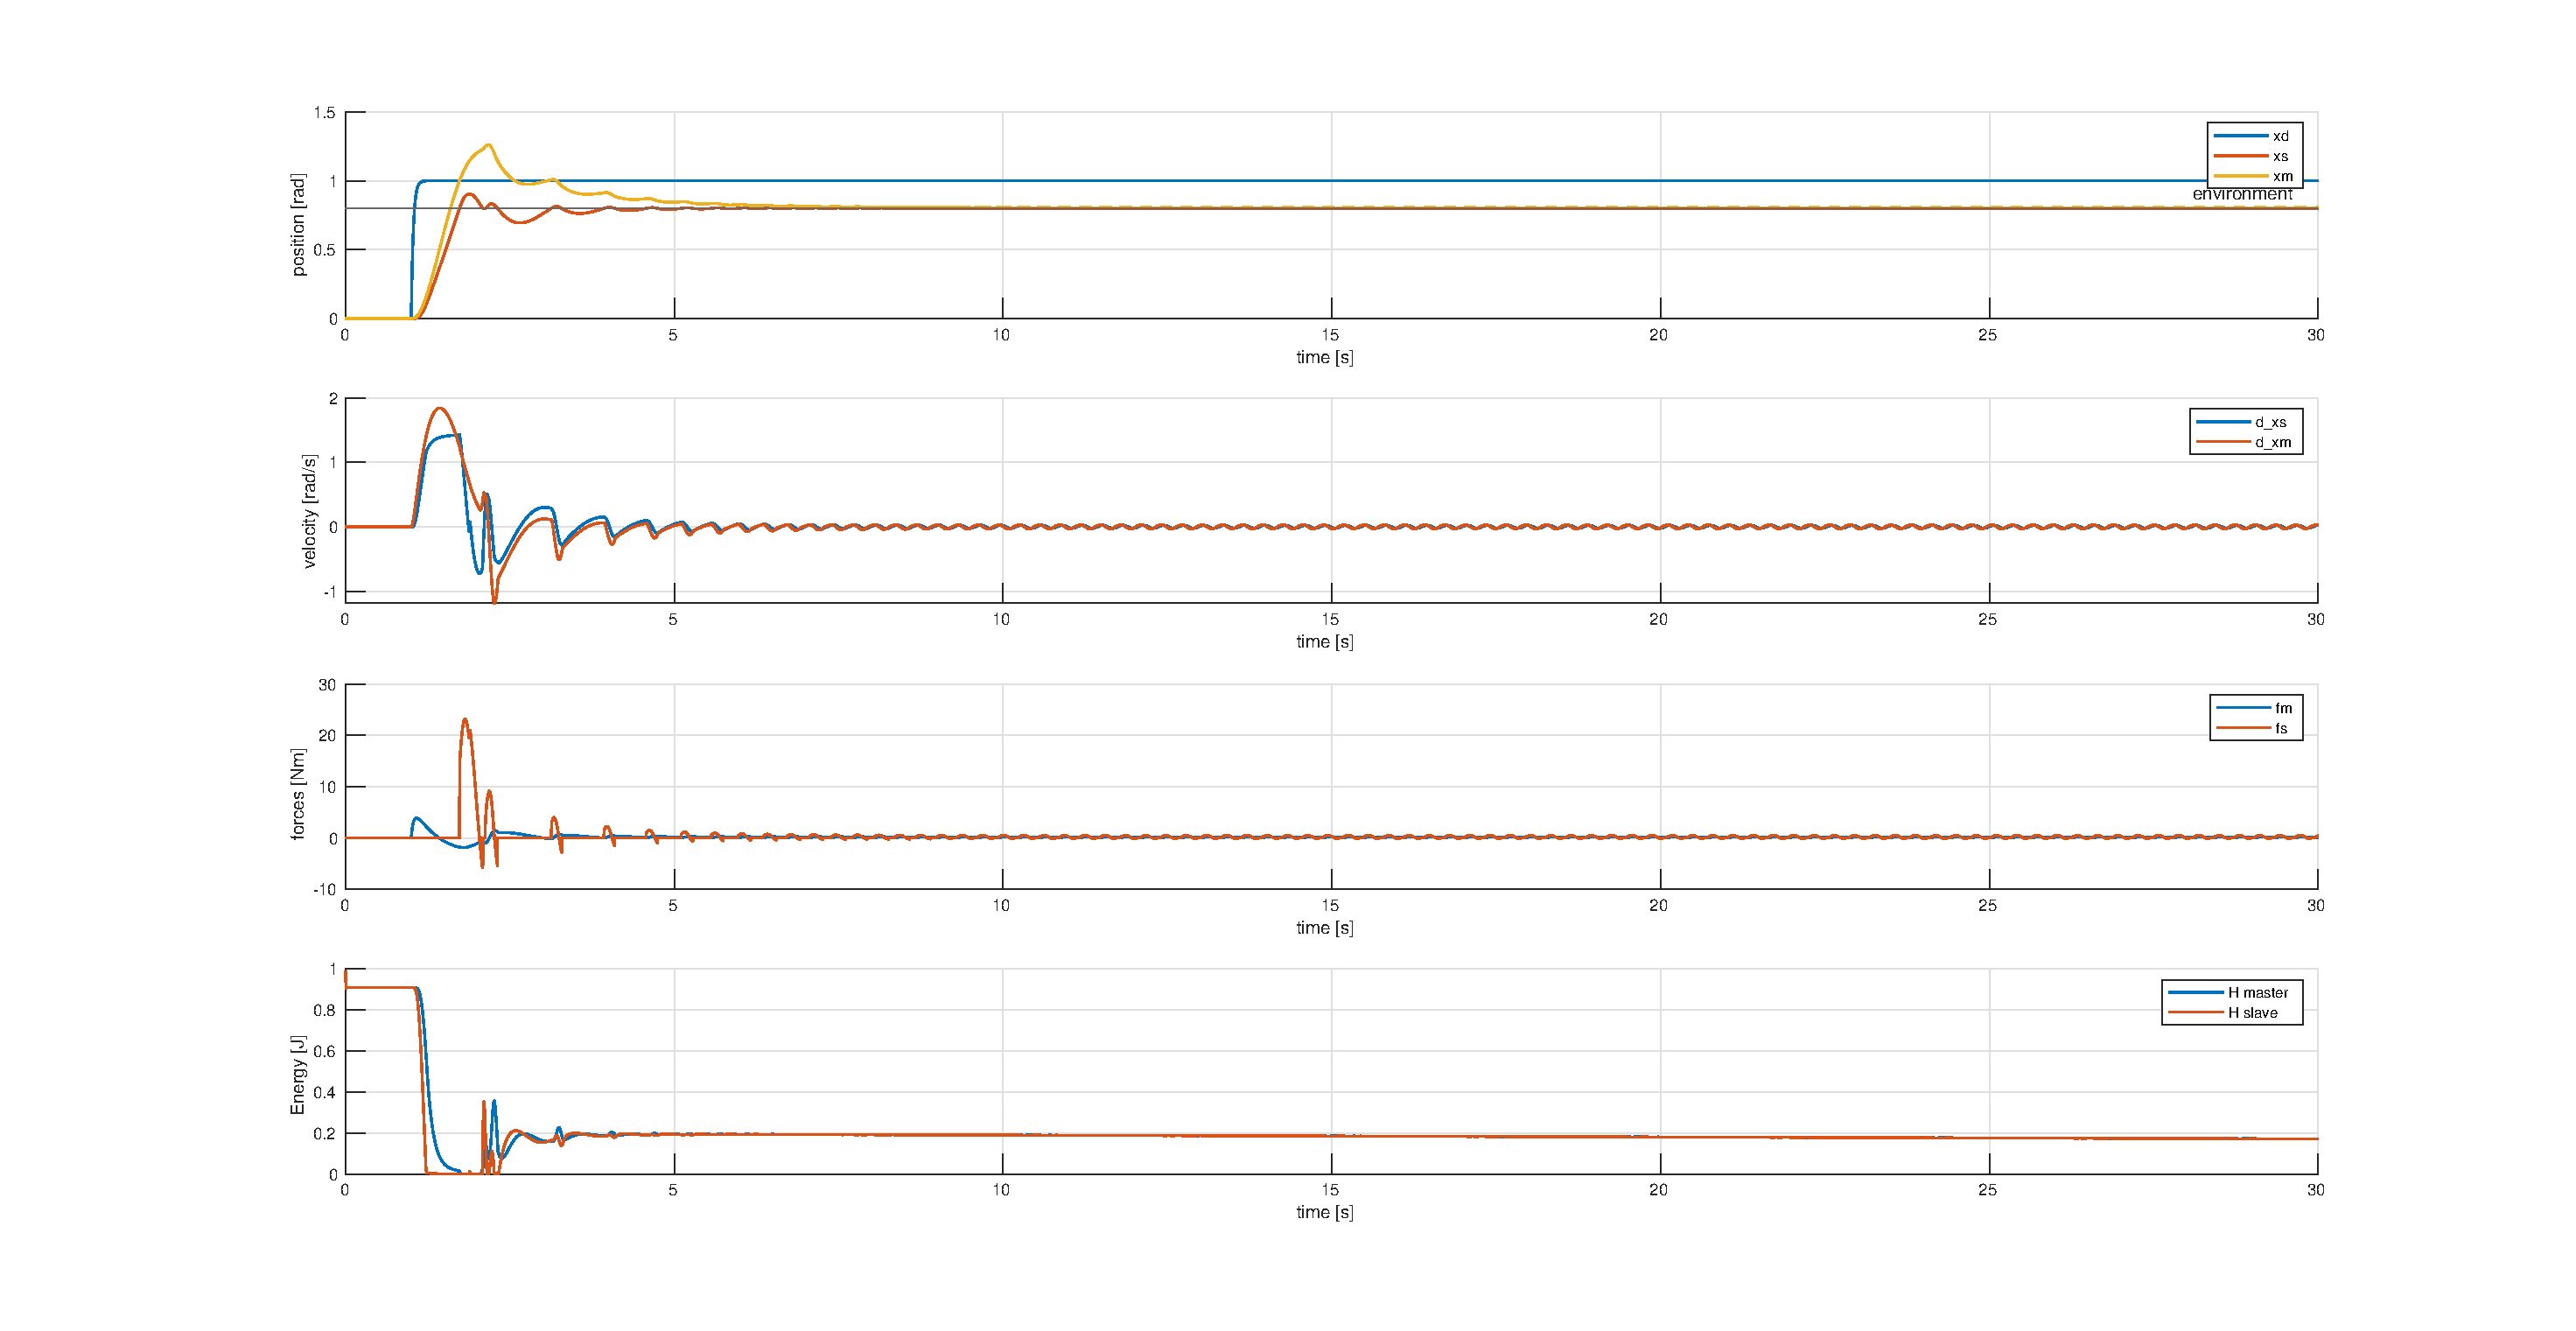
\includegraphics[scale=0.5]{images/energy_pf_step.eps}
    \end{center}
    \caption{Two-Layer bilateral architecture FP in contact at 0.8 with step reference. In order to produce this response the integral action from the human intention controller was removed.}
    \label{fig:energy_pf_step}
\end{figure}

\newpage
\subsection{Two-Layer bilateral architecture Position Position}
The idea of the PP architecture is to use the master and slave velocities measurements and use them as reference on the other side. In this way we have a velocity controller on both slave and master. In this scenario the two layer architecture Position-Position was evaluated with a delay of 10 time steps in the communication channel. The environment used is $B_e = 10$ and $K_e = 200$. 

\bigskip
In Figure \ref{fig:energy_pp_free} the free motion response of a sinusoidal reference is reported with proper tuning both at master and slave side.

\begin{figure}[H]
    \begin{center}
        \hspace*{-4.5cm}
        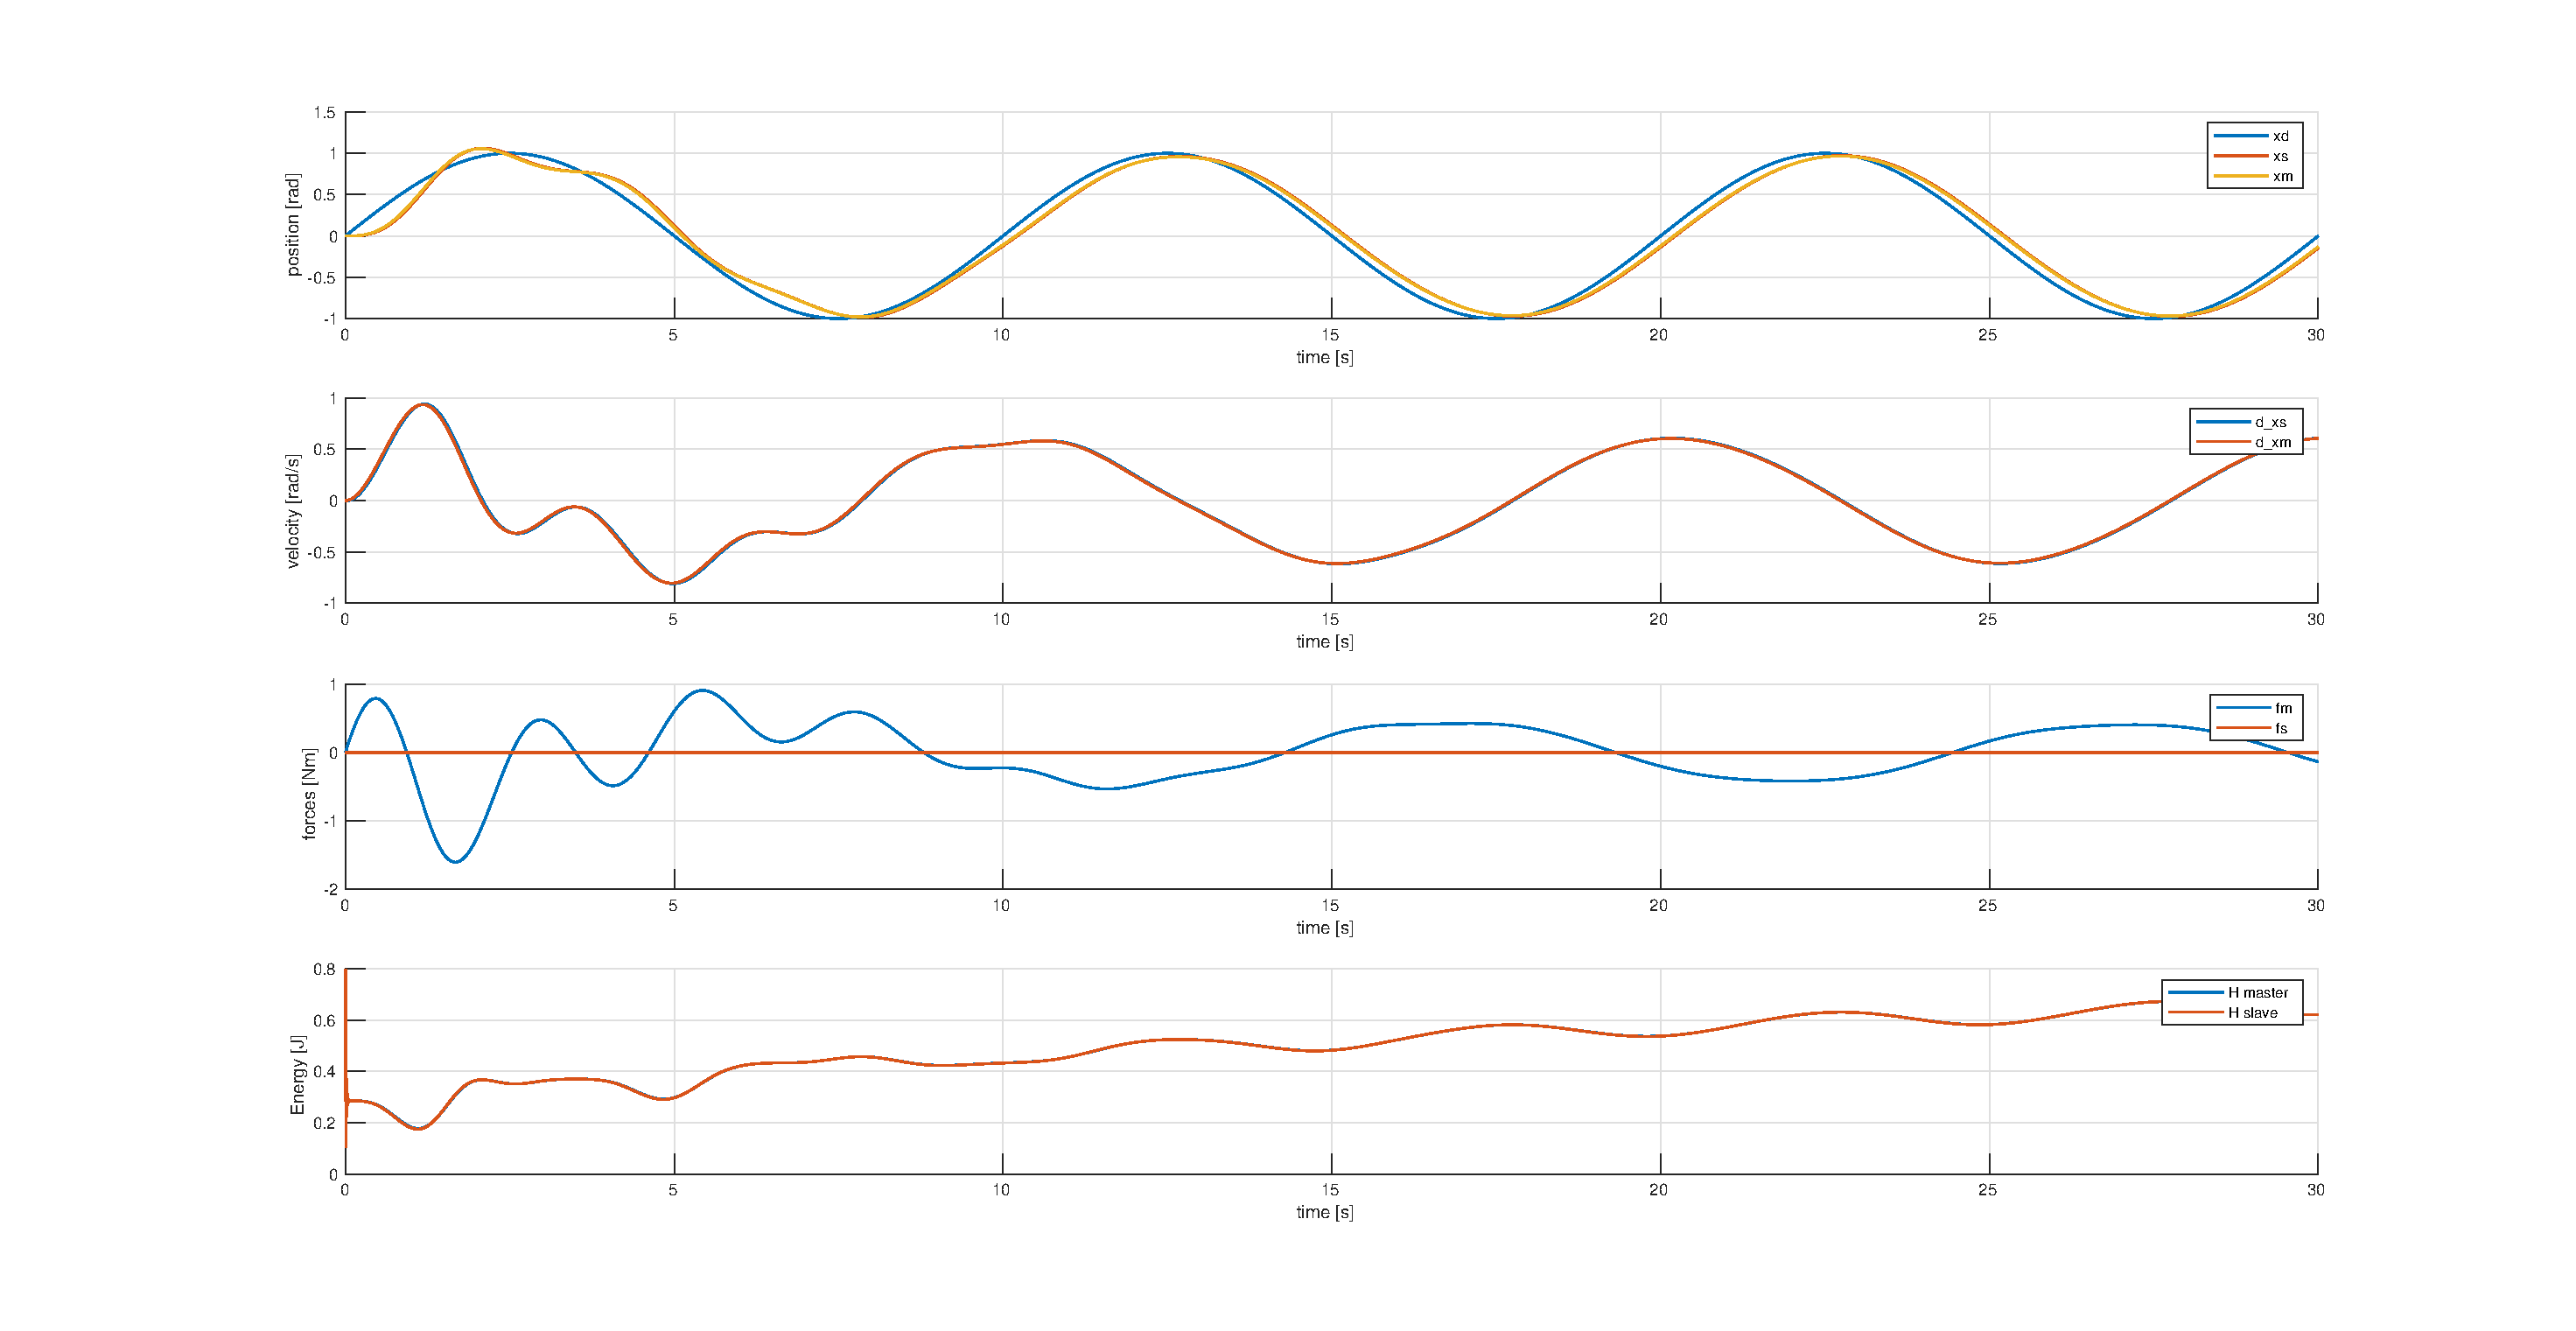
\includegraphics[scale=0.5]{images/energy_pp_free.eps}
    \end{center}
    \caption{Two-Layer bilateral architecture PP in free motion with energy in the tanks}
    \label{fig:energy_pp_free}
\end{figure}

\newpage
In Figure \ref{fig:energy_pp_contact} the contact plot of a sinusoidal reference is reported with proper tuning. Enough initial energy was set in the tanks to perform the task.

\begin{figure}[H]
    \begin{center}
        \hspace*{-4.5cm}
        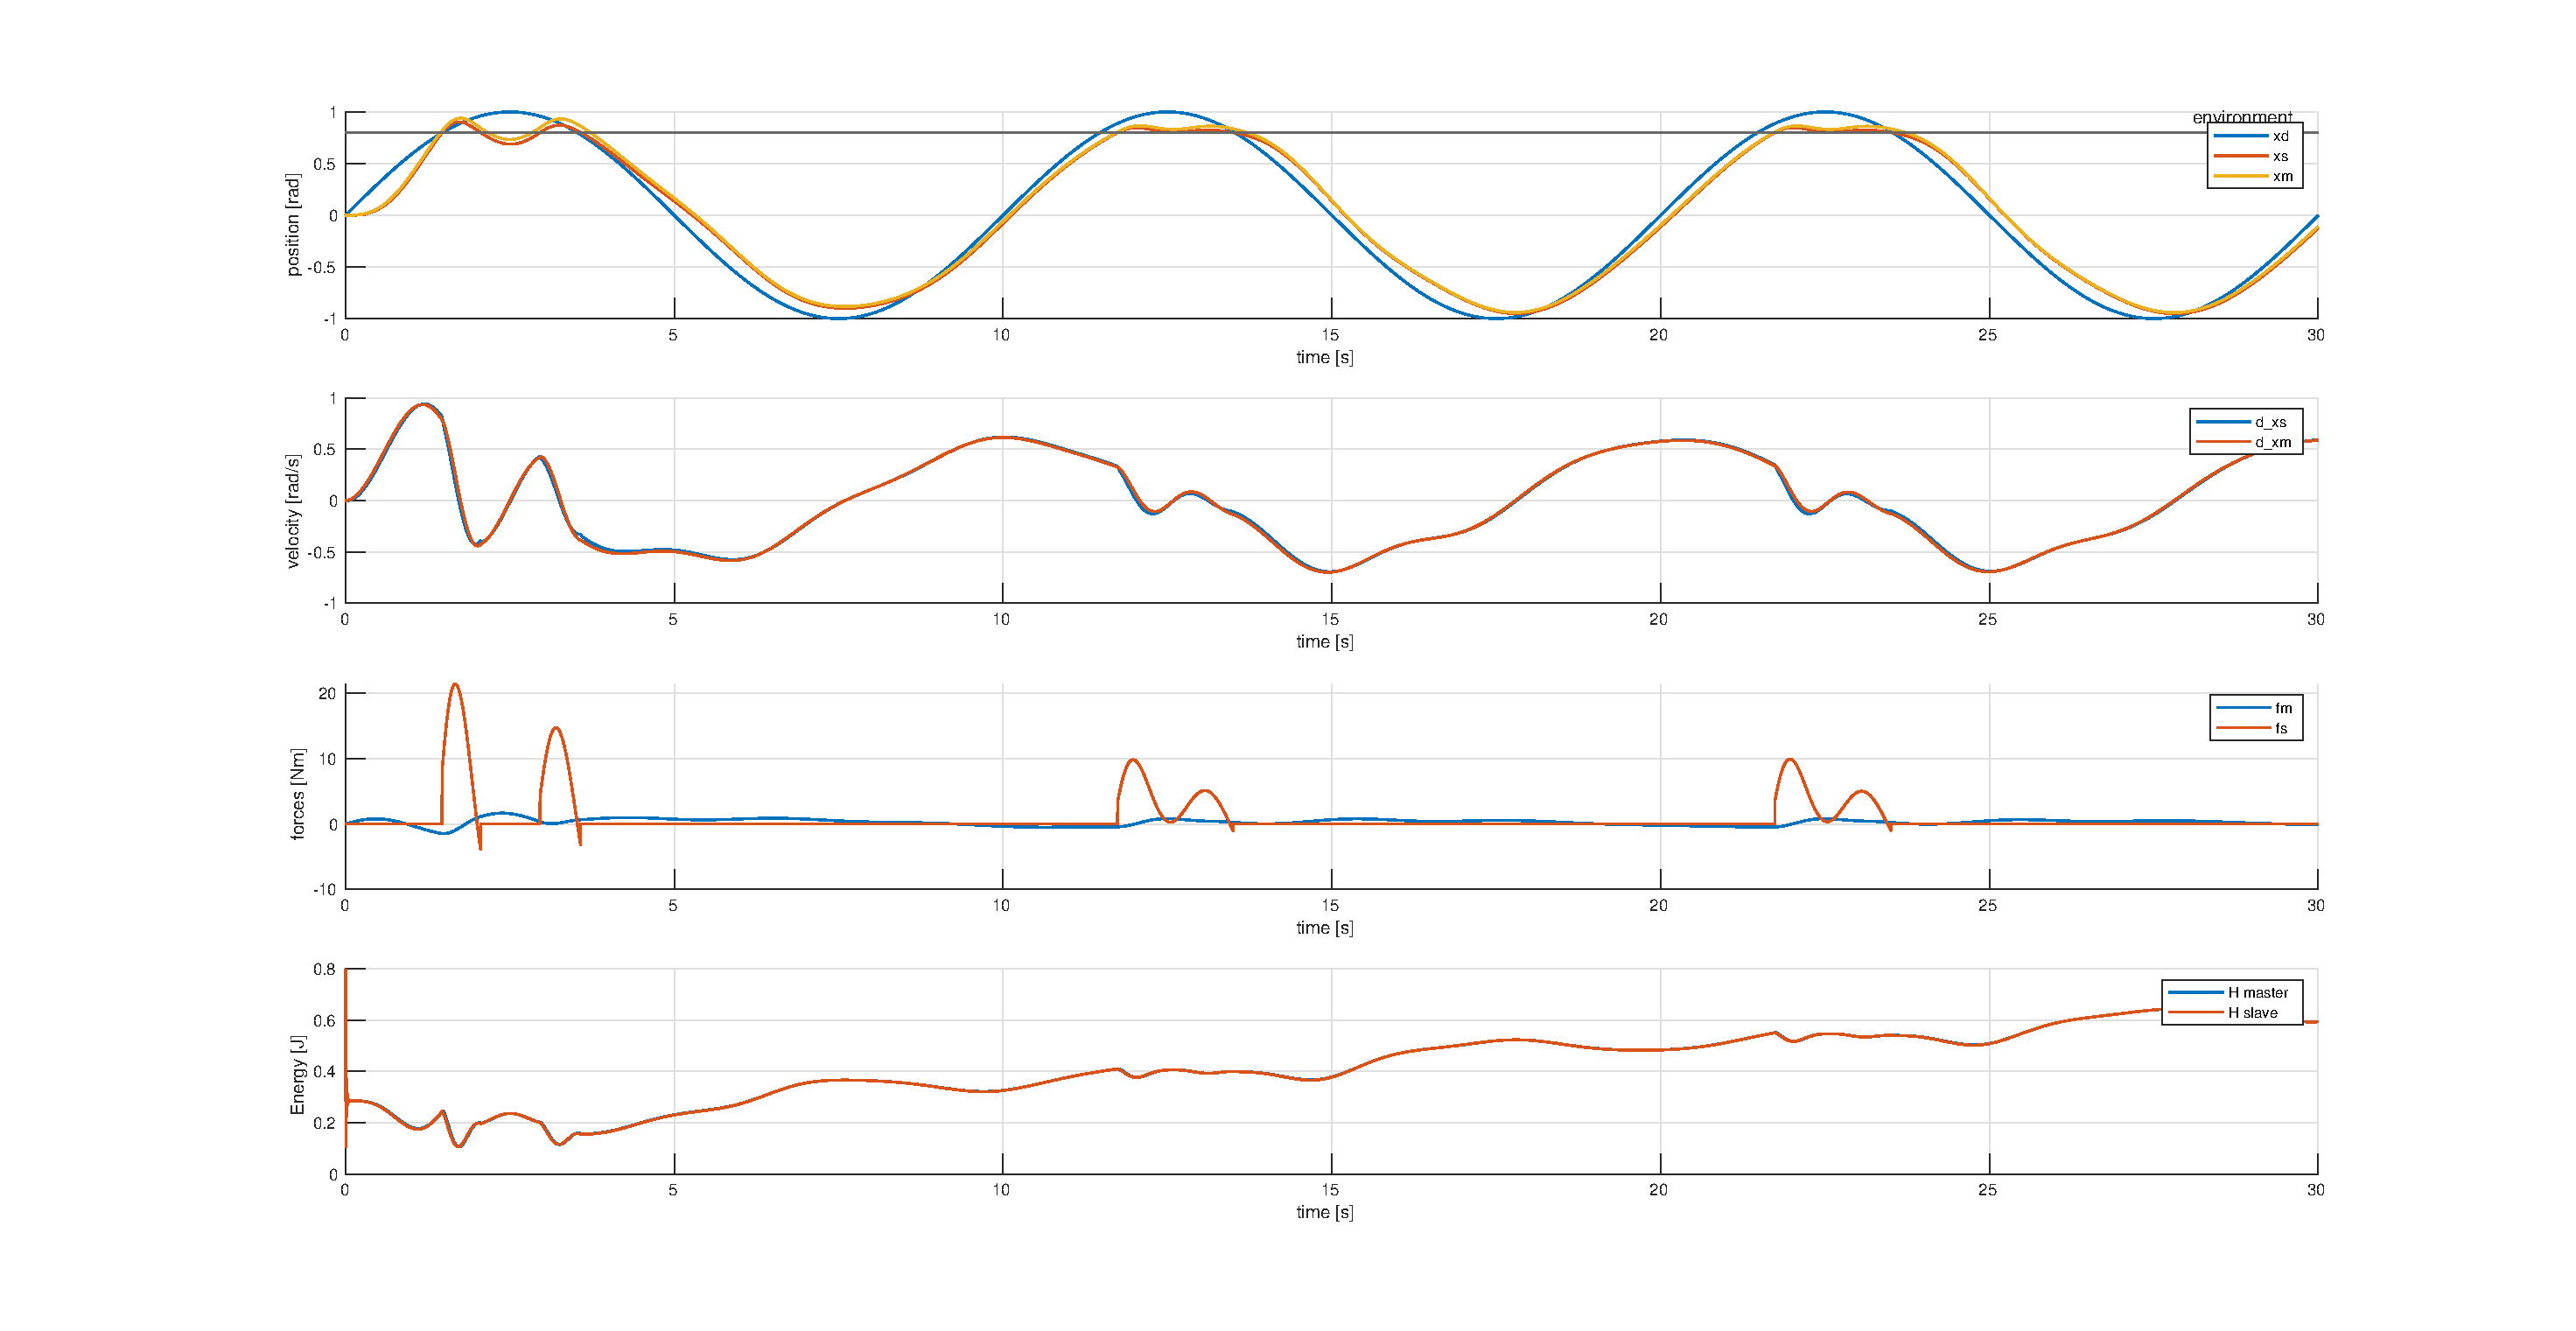
\includegraphics[scale=0.5]{images/energy_pp_contact.eps}
    \end{center}
    \caption{Two-Layer bilateral architecture PP in contact at 0.8}
    \label{fig:energy_pp_contact}
\end{figure}

The parameters used for the energy layer are $\alpha = 0.1$, $\beta = 0.01$ and the level for the TLC $H_d = 0.5$. However this values are indicative and were briefly adjusted in the various scenarios to obtain the related plots.
\bigskip

In Fig \ref{fig:energy_pp_no_energy} the actual effect of the passivity layer is reported when there is no initial energy. The passivity layer actually modulates the transparency command due to missing energy.

\begin{figure}[H]
    \hspace*{-4.5cm}
    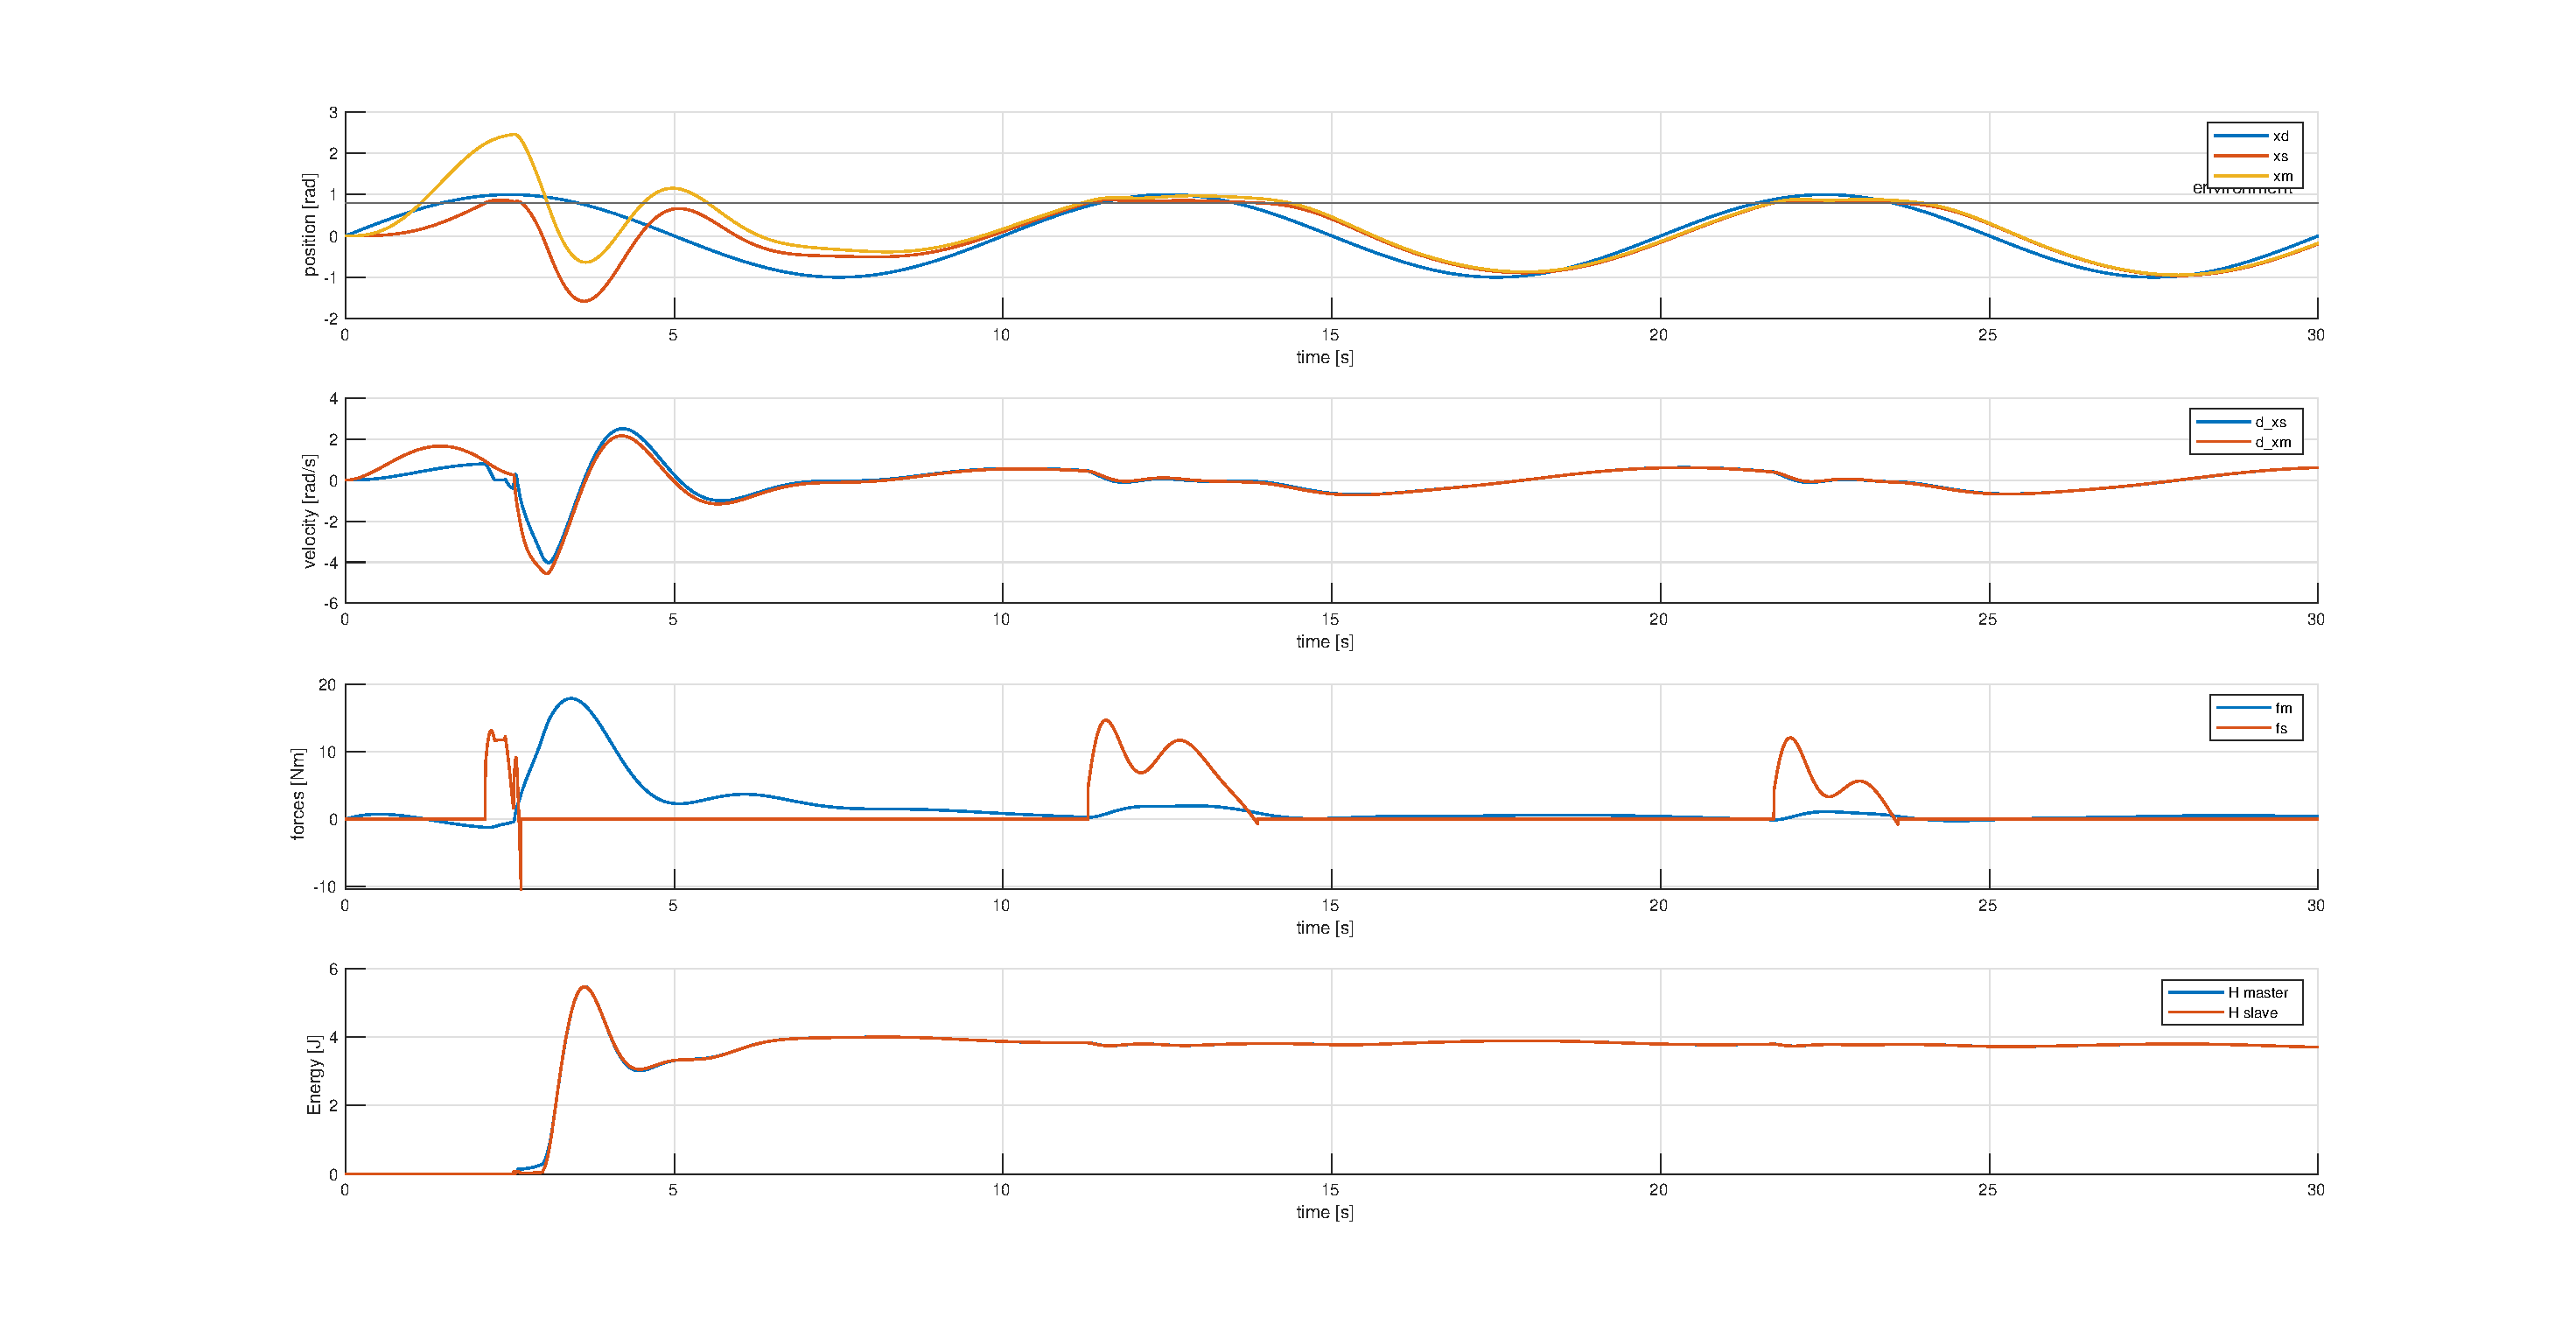
\includegraphics[scale=0.5]{images/energy_pp_no_energy.eps}
    \qquad
    \hspace*{-1.5cm}
    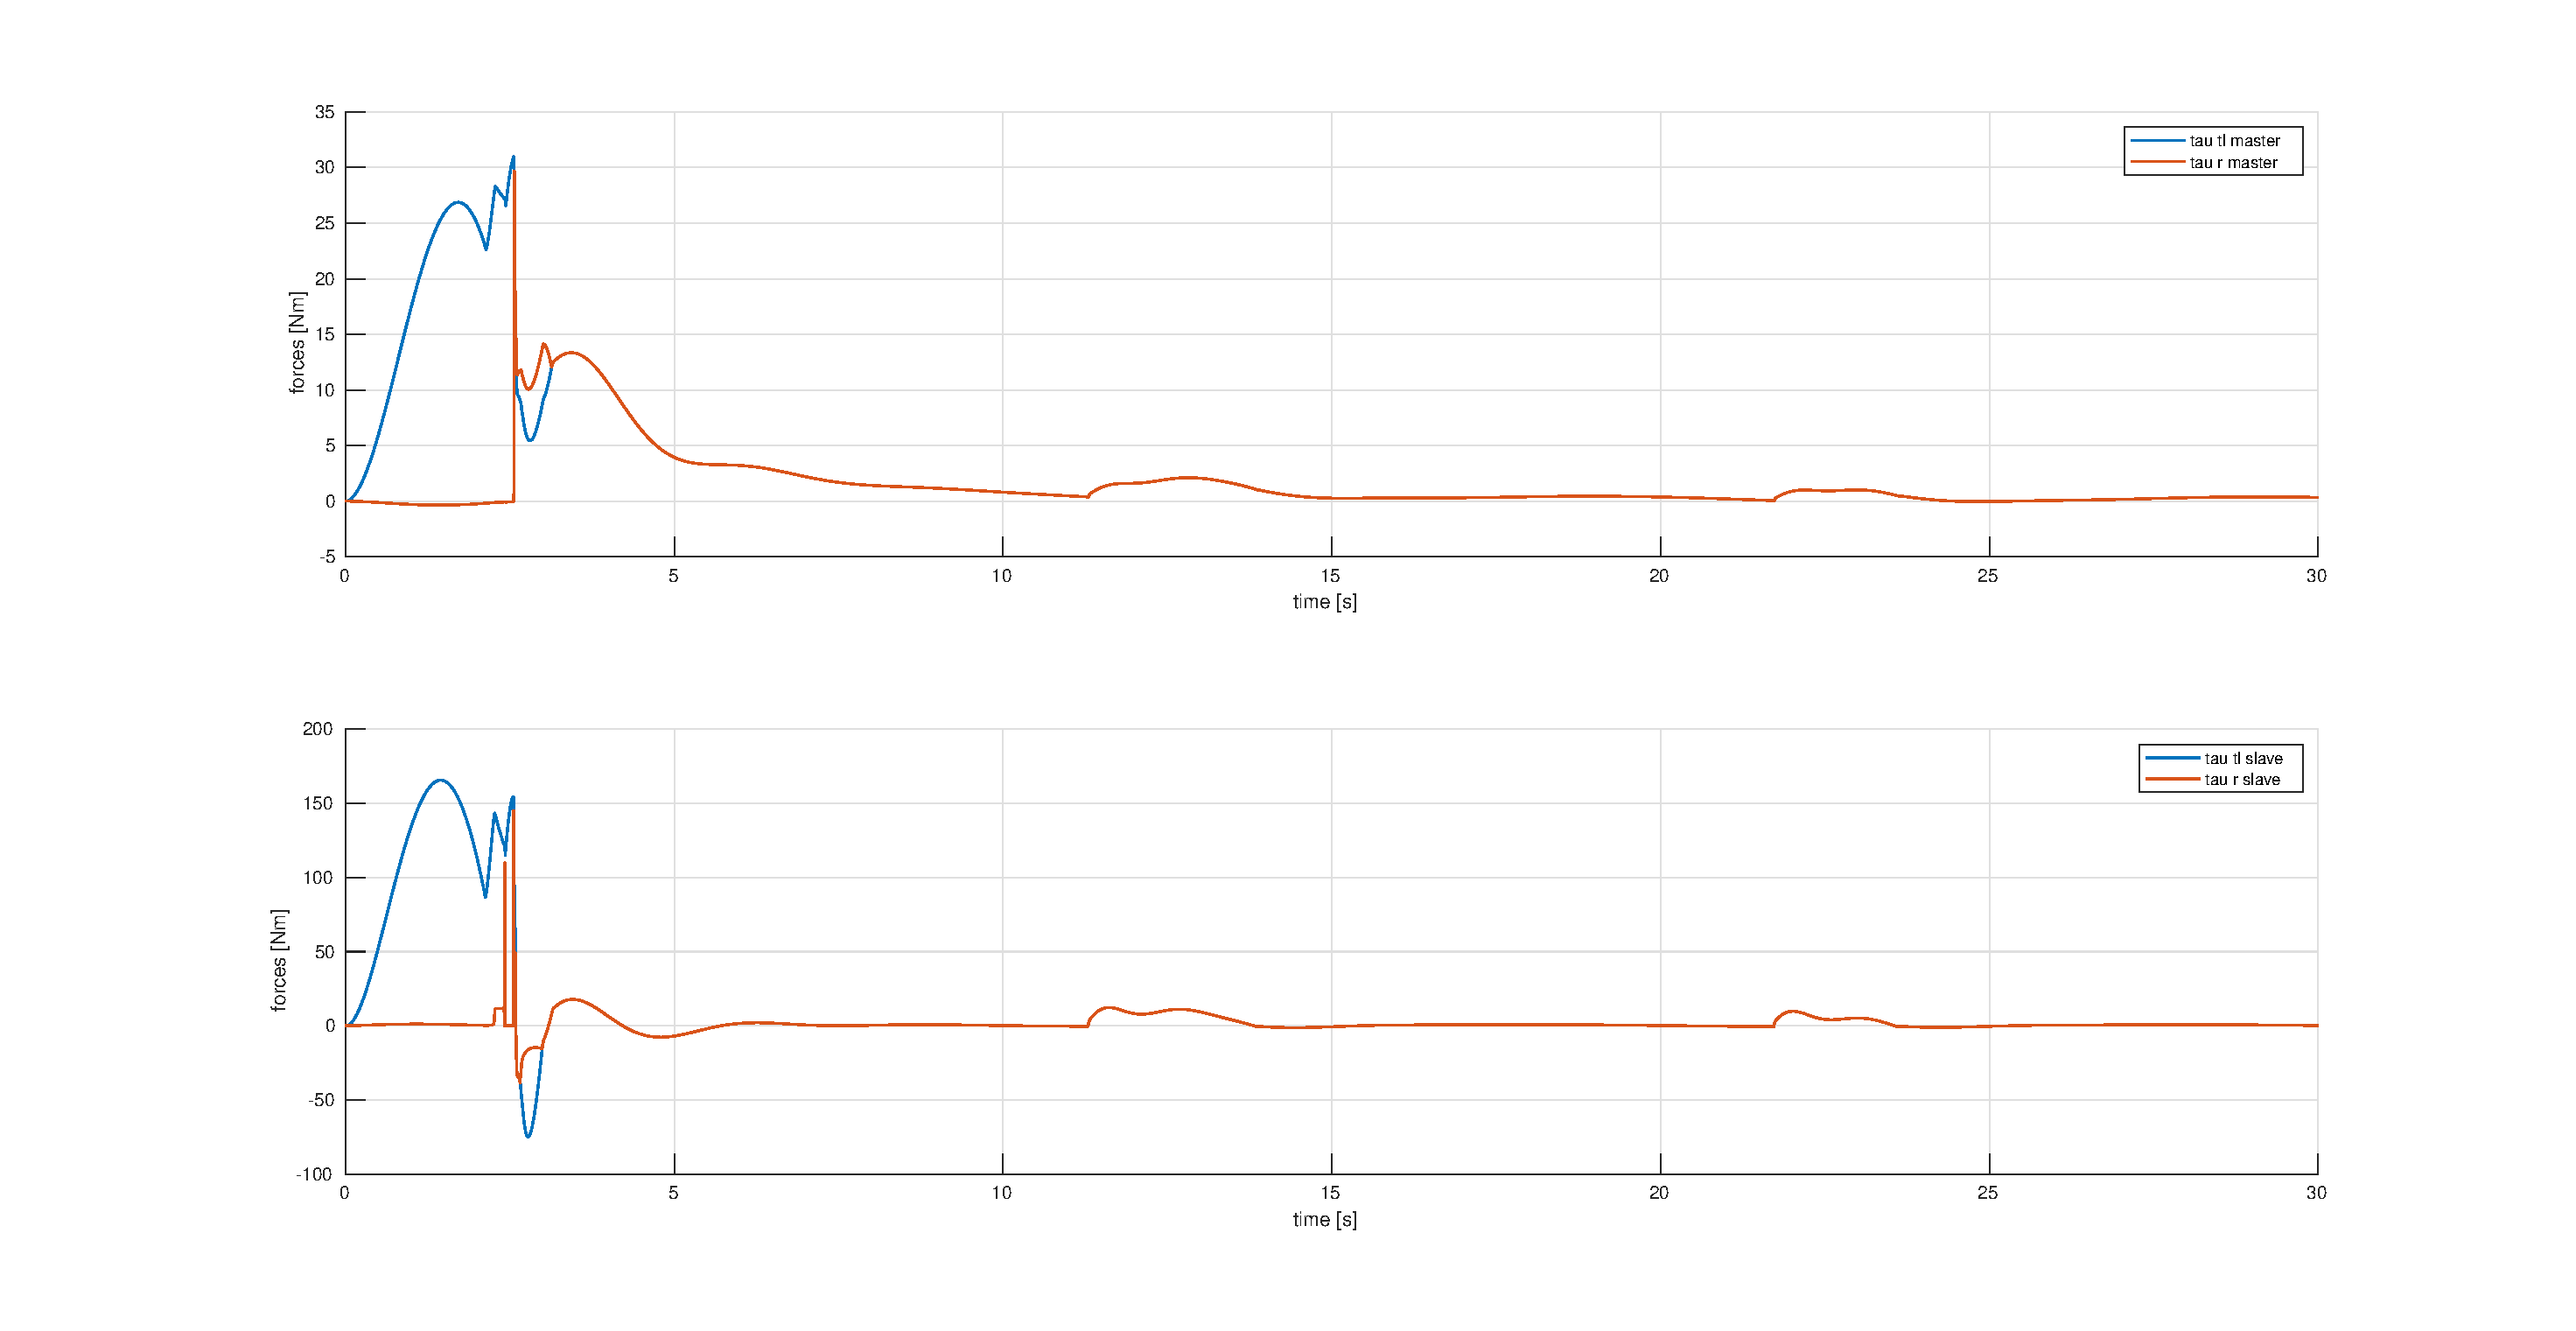
\includegraphics[scale=0.4]{images/energy_pp_tau.eps}
    \caption{Top: Two-Layer bilateral architecture PP in contact at 0.8 with no initial energies. Bottom: Comparison of the torques produced by the transparency and the passivity layer without initial energy in the tanks}
    \label{fig:energy_pp_no_energy}
\end{figure}


\begin{figure}[H]
    \hspace*{-4.5cm}
    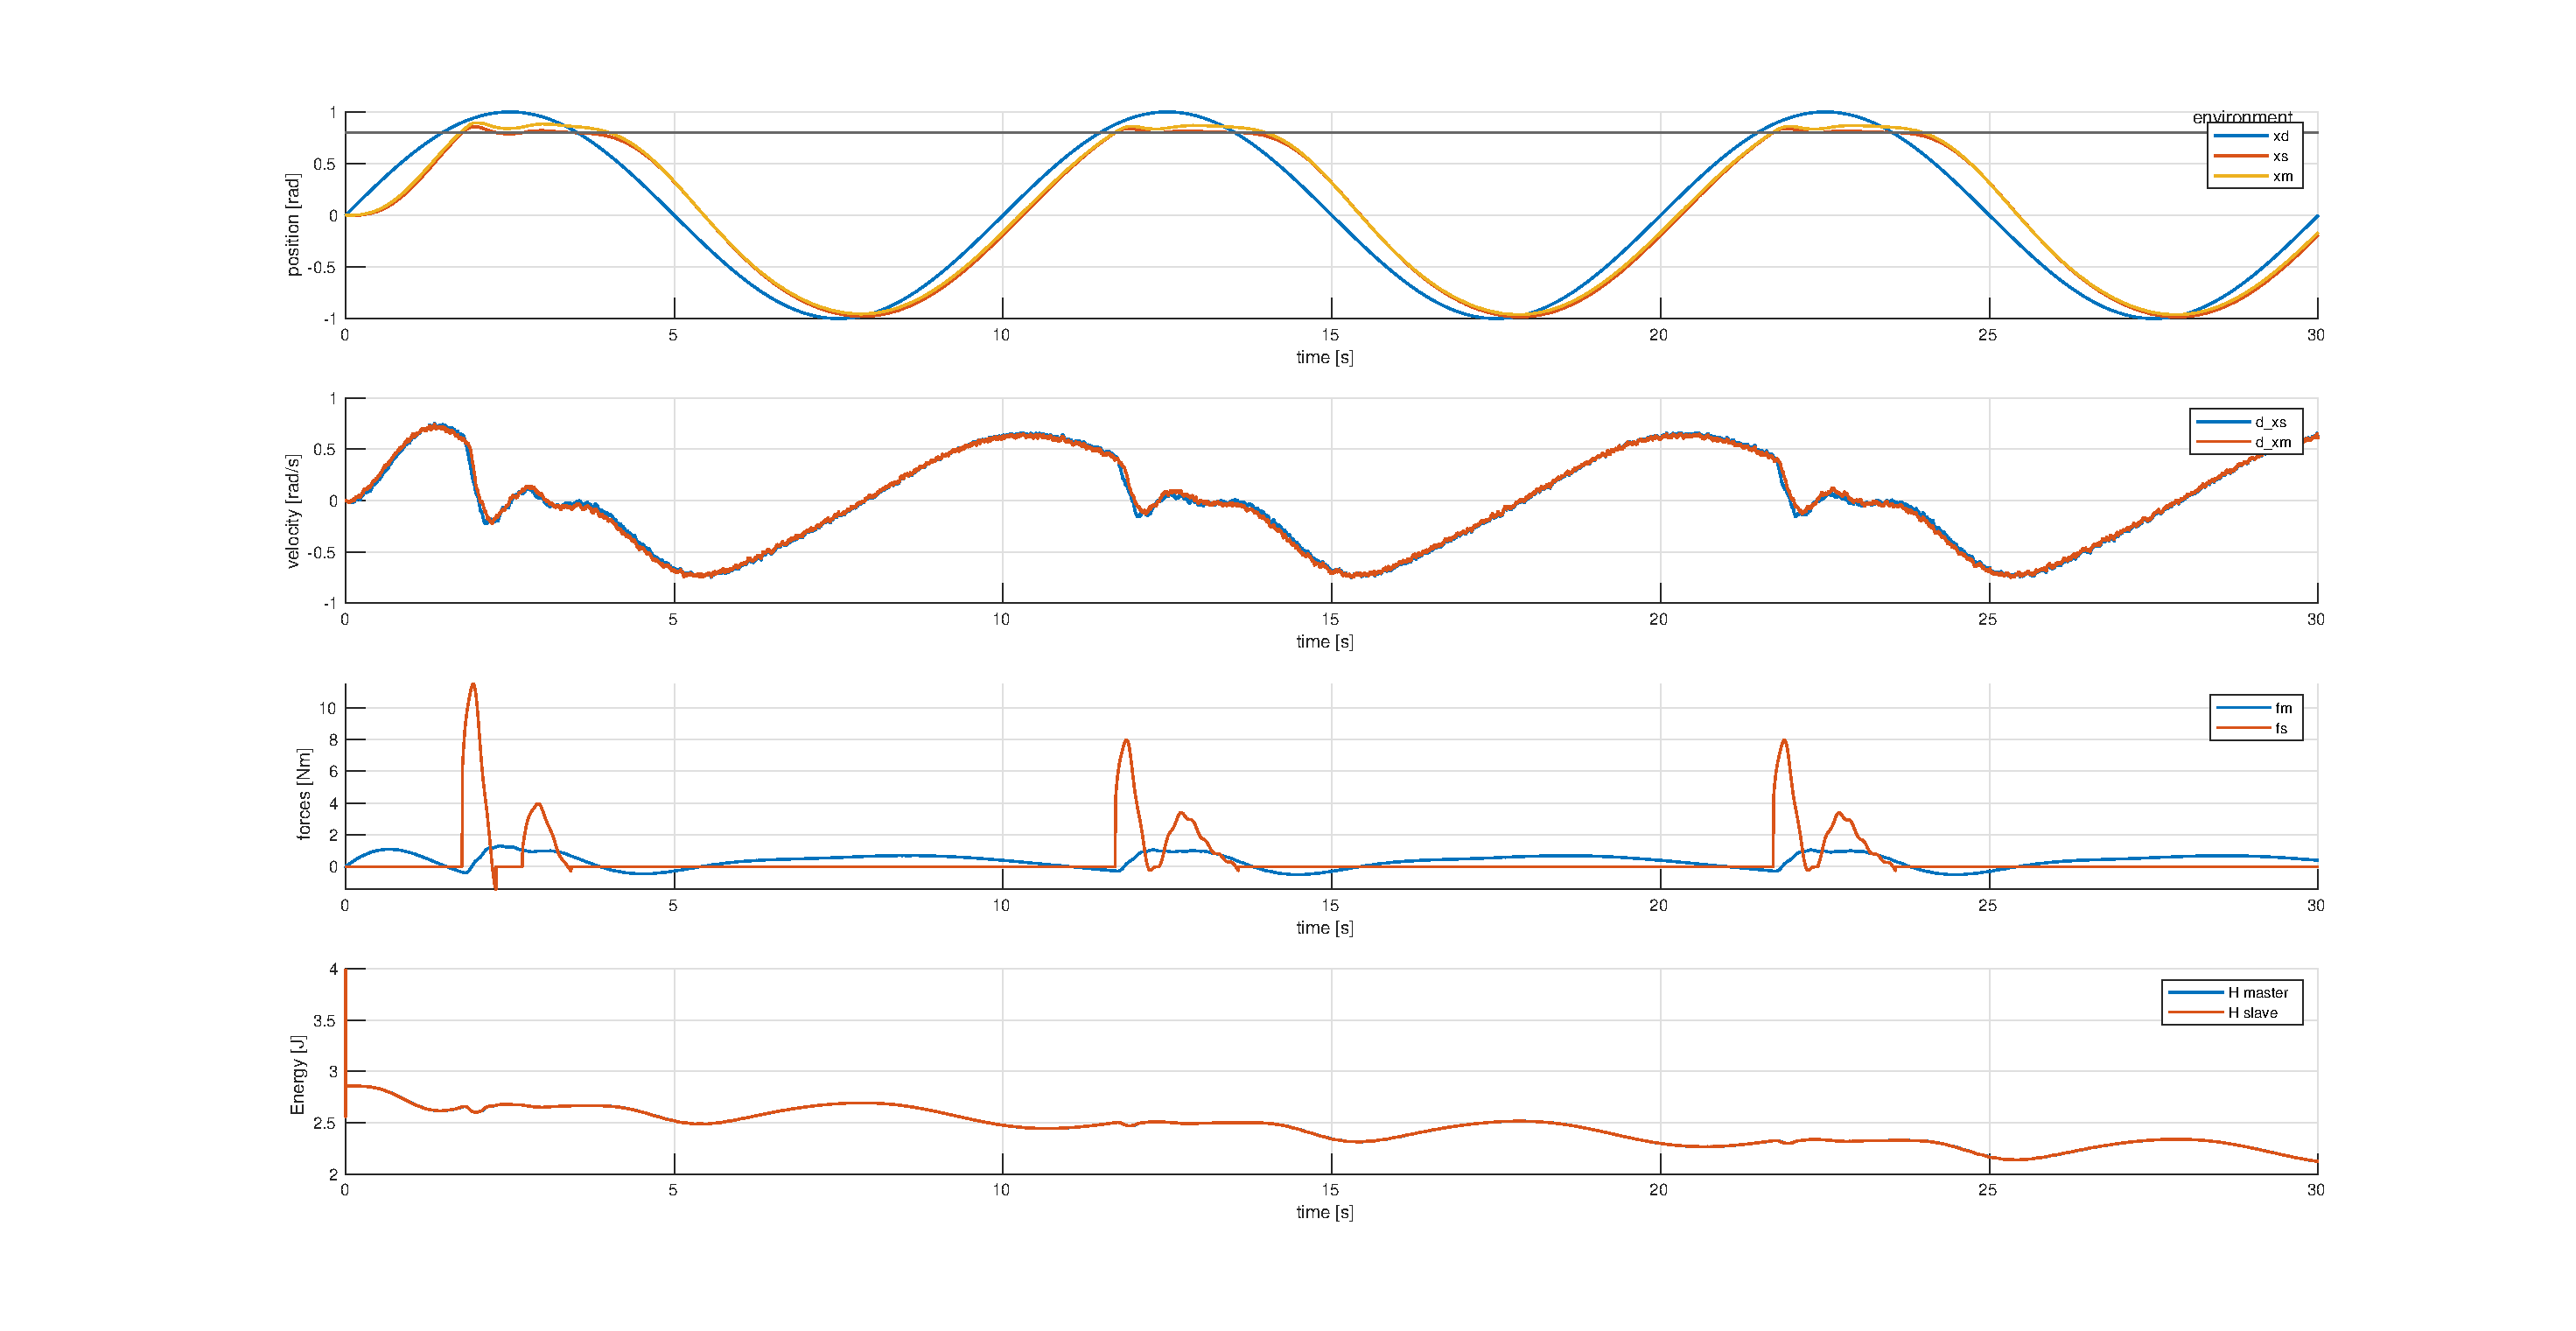
\includegraphics[scale=0.5]{images/energy_pp_kalman.eps}
    \qquad
    \hspace*{-1.5cm}
    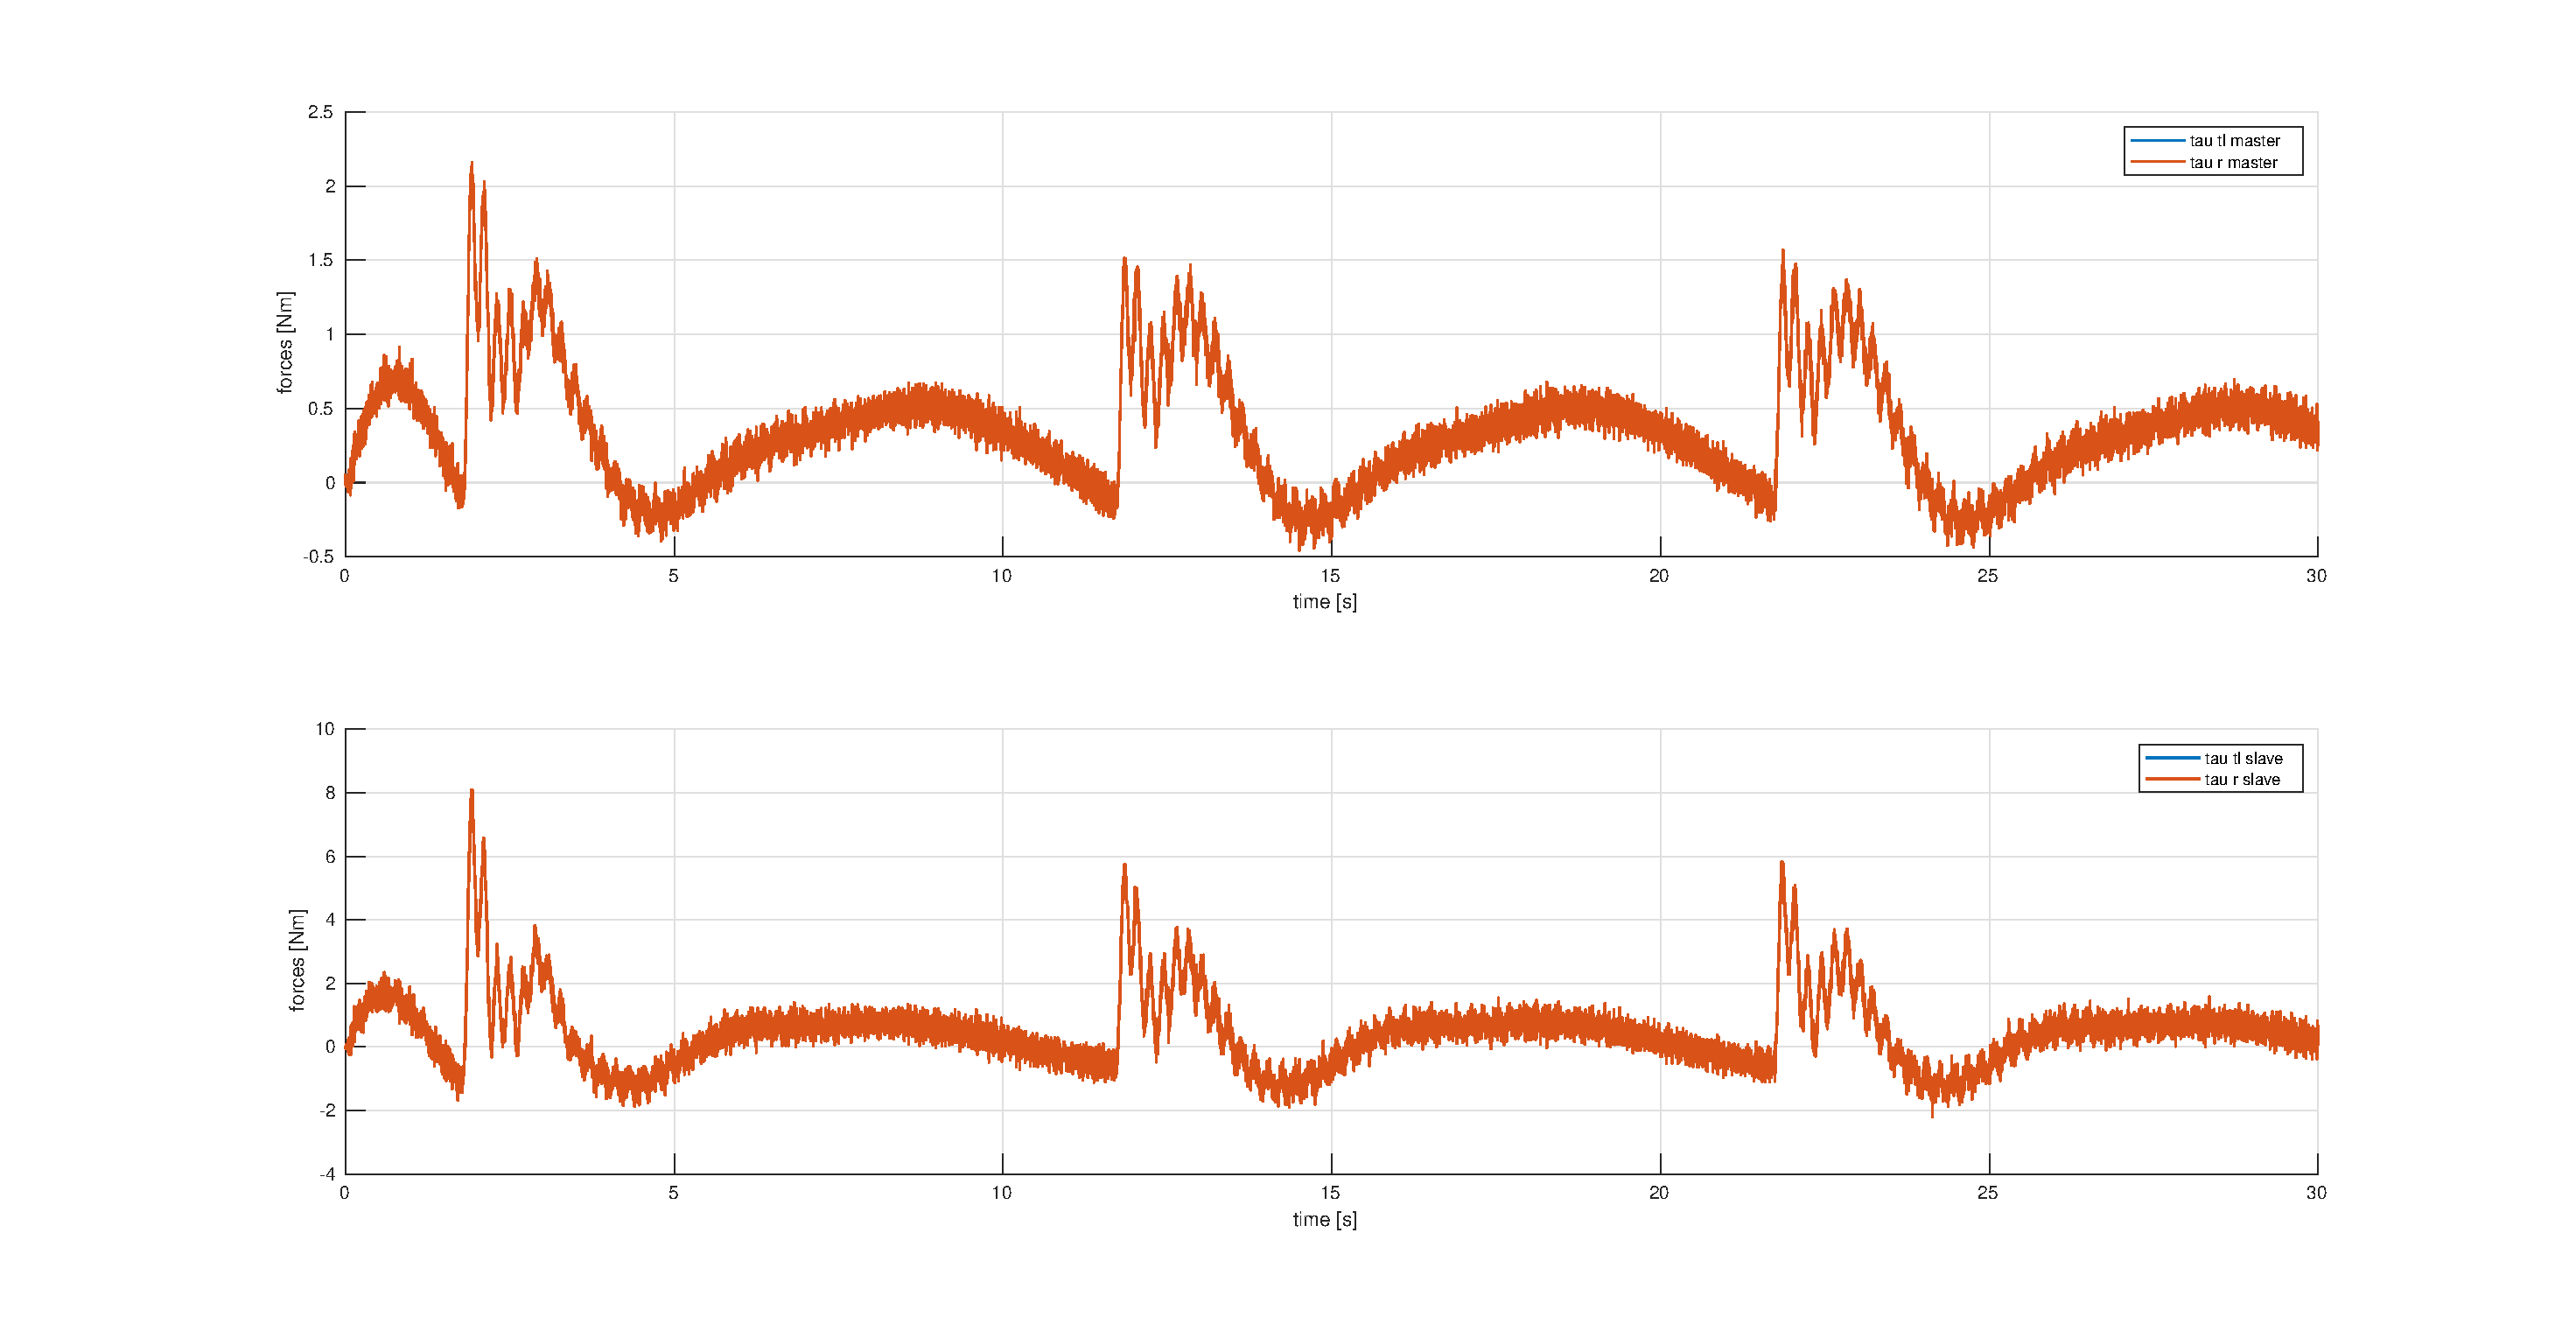
\includegraphics[scale=0.4]{images/energy_pp_tau_kalman.eps}
    \caption{Top: Two-Layer architecture PP in contact at 0.8 with kalman filters. Bottom: Comparison of the torques produced by the transparency and the passivity layer with full initial energies}
    \label{fig:energy_pp_kalman}
\end{figure}
\newpage

Finally, In Figure \ref{fig:energy_pp_step} the step response of the architecture is reported.

\begin{figure}[H]
    \begin{center}
        \hspace*{-4.5cm}
        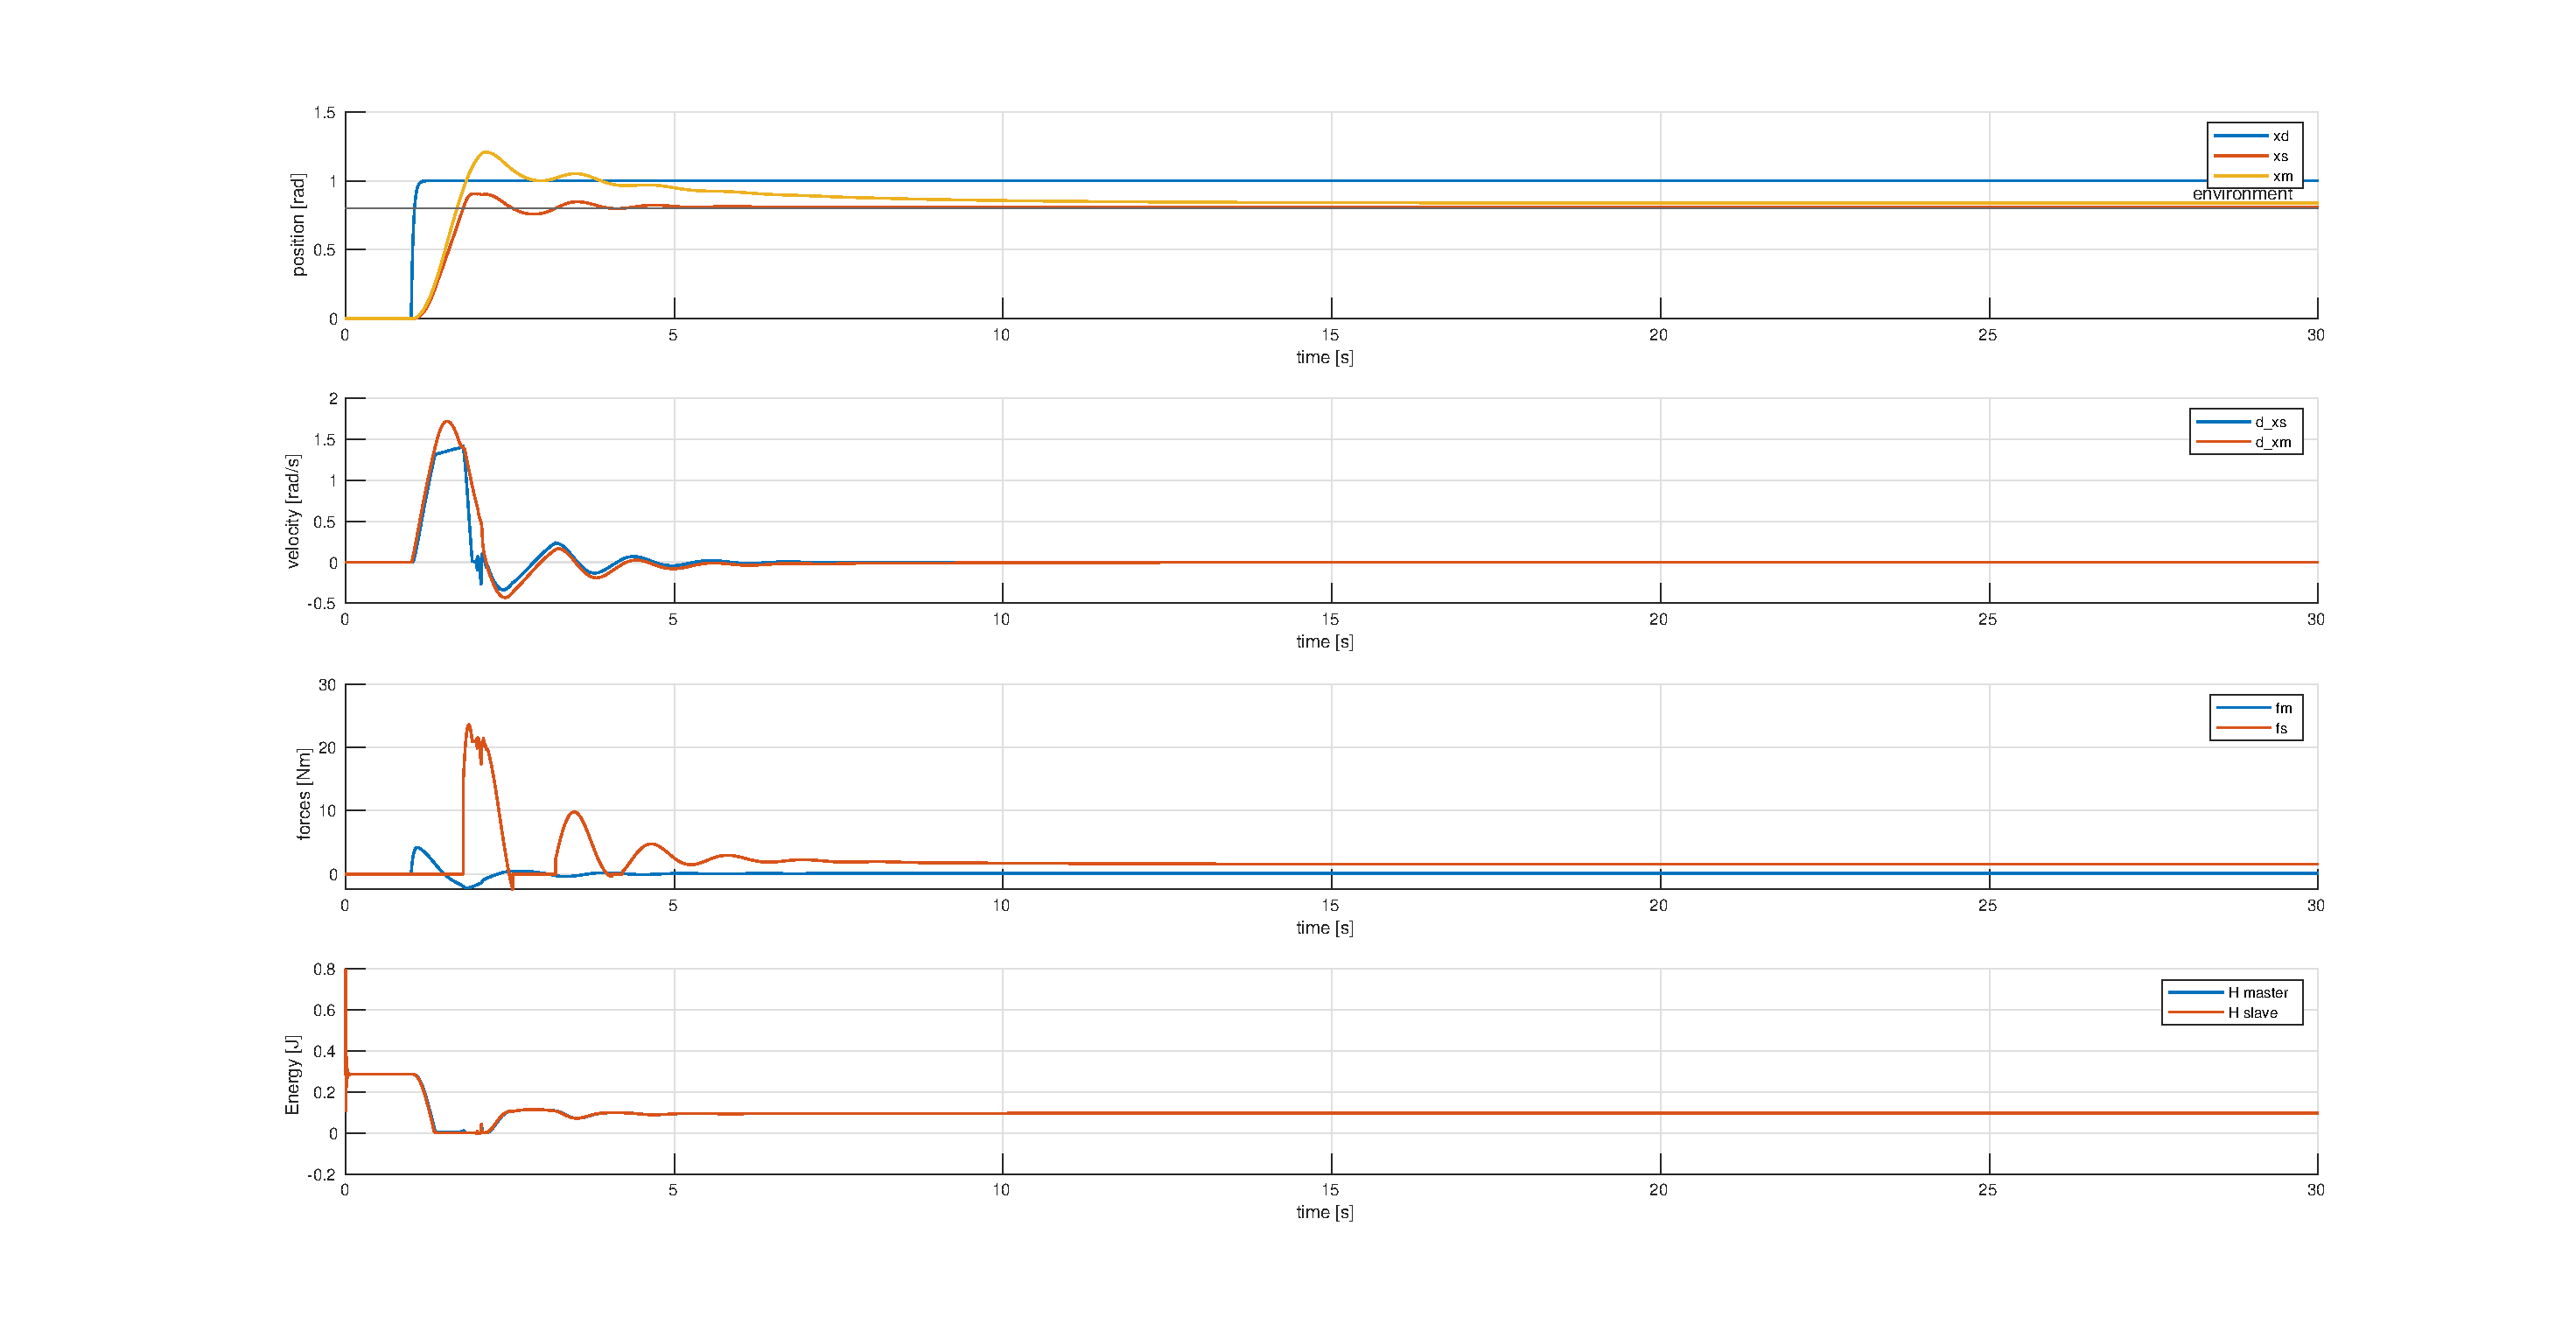
\includegraphics[scale=0.5]{images/energy_pp_step.eps}
    \end{center}
    \caption{Two-Layer bilateral architecture PP in contact at 0.8 with step reference. In order to produce this response the integral action from the human intention controller was removed.}
    \label{fig:energy_pp_step}
\end{figure}

\begin{thebibliography}{100}
    \addtolength{\leftmargin}{0.2in}
    \setlength{\itemindent}{-0.2in}

    \bibitem{Lawrence93} Dale A. Lawrence "Stability and Transparency in Bilateral Teleoperation" 1993
    \bibitem{Niemeyer91} Gunter Niemeyer and Jean-Jacques E. Slotine "Stable Adaptive Teleoperation" 1991
    \bibitem{Franken11} M. Franken, S. Stramigioli, S. Misra, C. Secchi, A. Macchelli "Bilateral Telemanipulation With Time Delays: A Two-Layer Approach Combining Passivity and Transparency" 2011
\end{thebibliography}

\end{document}
